%% LyX 2.3.7 created this file.  For more info, see http://www.lyx.org/.
%% Do not edit unless you really know what you are doing.
\documentclass[11pt,oneside,czech,american]{book}
\usepackage[T1]{fontenc}
\usepackage[utf8]{inputenc}
\usepackage[a4paper]{geometry}
\geometry{verbose,tmargin=4cm,bmargin=3cm,lmargin=3cm,rmargin=2cm,headheight=0.8cm,headsep=1cm,footskip=0.5cm}
\pagestyle{headings}
\setcounter{secnumdepth}{3}

\usepackage{url}
\usepackage{amsmath}
\usepackage{amsthm}
\usepackage{amssymb}
\usepackage{graphicx}
\usepackage{setspace}
\usepackage{placeins}
% \usepackage[hidelinks]{hyperref}
\usepackage{minted}
\usepackage{amsmath}
\usepackage{amsfonts} 
\usepackage{physics}
\usepackage{graphicx}
\usepackage{hyperref}
\usepackage{mathrsfs}
\usepackage{algpseudocode}
\usepackage{algorithm}
\usepackage{xcolor}
\usepackage{subcaption}
\usepackage{nicematrix} %Block matrices
% \usepackage[colorlinks=true, allcolors=blue]{hyperref}
\usepackage{titlesec}
\usepackage{mathtools}

\usepackage{caption}
\usepackage{array}
\usepackage{booktabs}
\usepackage{hyperref}
\hypersetup{colorlinks,linkcolor={red},citecolor={blue},urlcolor={blue}} 

\usepackage[
    backend=biber,
    style=alphabetic
]{biblatex}

\addbibresource{references.bib}

\newcolumntype{P}[1]{>{\centering\arraybackslash}p{#1}}

\newenvironment{codelisting}{\captionsetup{type=listing}}{}
%\SetupFloatingEnvironment{listing}{name=Source Code}

% \setcounter{secnumdepth}{4}

% \titleformat{\paragraph}
% {\normalfont\normalsize\bfseries}{\theparagraph}{1em}{}
% \titlespacing*{\paragraph}
% {0pt}{3.25ex plus 1ex minus .2ex}{1.5ex plus .2ex}

\newcommand{\TODO}[1]{{\color{red}[#1]}}
\newcommand{\todoref}[1][]{\TODO{ref: #1}}
\newcommand{\NOTE}[1]{{\color{green}[#1]}}
\newcommand{\Timeint}[0]{\mathcal{T}}
\newcommand{\Domain}[0]{\Omega}
\newcommand{\R}[0]{{\mathbb R}}
\newcommand{\Nats}[0]{{\mathbb N}}
\newcommand{\der}[2]{\frac{\partial #1}{\partial #2}}
\newcommand{\dert}[1]{\der{#1}{t}}
\newcommand{\ddt}[1]{\frac{\dd {#1}}{\dd t}}
% \newcommand{\dx}[0]{\Delta\mbox{x}}
% \newcommand{\dy}[0]{\Delta\mbox{y}}
% \newcommand{\dt}[0]{\Delta\mbox{t}}
\newcommand{\dx}[0]{\Delta x}
\newcommand{\dy}[0]{\Delta y}
\newcommand{\dt}[0]{\Delta t}
\newcommand{\mat}[1]{#1}
\newcommand{\vvskip}[0]{\vspace{\baselineskip} \noindent}
\newcommand{\Cells}[0]{\mathcal{M}}
\newcommand{\Faces}[0]{\mathcal{\varepsilon}}
\newcommand{\Centroids}[0]{\mathcal{P}}
\newcommand{\BoundCentroids}[0]{\mathcal{B}}
\newcommand{\laplace}[0]{\laplacian}
\newcommand{\bigfrac}[2]{\frac{\displaystyle #1}{\displaystyle #2}}
\newcommand{\code}[1]{\texttt{#1}}
\newcommand{\dlaplace}[0]{\laplace_d}
\newcommand{\dnabla}[0]{\nabla_d}

\DeclarePairedDelimiter\ceil{\lceil}{\rceil}
\DeclarePairedDelimiter\floor{\lfloor}{\rfloor}

% \newcommand{\dd}[0]{\text{d}}

\newcommand{\clim}[1]{\lim\limits_{#1}}
\newcommand{\cinf}[1]{\inf\limits_{#1}}
\newcommand{\csup}[1]{\sup\limits_{#1}}

\newcommand{\halflimlike}[2]{\raisebox{0.5ex}{\scalebox{0.8}{$\displaystyle #1\limits_{#2}\;$}}}
\newcommand{\halflim}[1]{\halflimlike{\lim}{#1}}
\newcommand{\halfinf}[1]{\halflimlike{\inf}{#1}}
\newcommand{\halfsup}[1]{\halflimlike{\sup}{#1}}

\newlength{\subfigwidth}

\makeatletter
%%%%%%%%%%%%%%%%%%%%%%%%%%%%%% Textclass specific LaTeX commands.
\newenvironment{lyxlist}[1]
	{\begin{list}{}
		{\settowidth{\labelwidth}{#1}
		 \setlength{\leftmargin}{\labelwidth}
		 \addtolength{\leftmargin}{\labelsep}
		 \renewcommand{\makelabel}[1]{##1\hfil}}}
	{\end{list}}

%%%%%%%%%%%%%%%%%%%%%%%%%%%%%% User specified LaTeX commands.
%% Font setup: please leave the LyX font settings all set to 'default'
%% if you want to use an_y of these packages:

%% Use Times New Roman font for text and Belleek font for math
%% Please make sure that the 'esint' package is turned off in the
%% 'Math options' page.
% \usepackage[varg]{txfonts}

%% Use Utopia text with Fourier-GUTenberg math
%\usepackage{fourier}

%% Bitstream Charter text with Math Design math
%\usepackage[charter]{mathdesign}

%%---------------------------------------------------------------------

%% Make the multiline figure/table captions indent so that the second
%% line "hangs" right below the first one.
%\usepackage[format=hang]{caption}

%% Indent even the first paragraph in each section
\usepackage{indentfirst}

%%---------------------------------------------------------------------

\usepackage{pdfpages}

%%---------------------------------------------------------------------

%% Disable page numbers in the TOC. LOF, LOT (TOC automatically
%% adds \thispagestyle{chapter} if not overriden
%\addtocontents{toc}{\protect\thispagestyle{empty}}
%\addtocontents{lof}{\protect\thispagestyle{empty}}
%\addtocontents{lot}{\protect\thispagestyle{empty}}

%% Shifts the top line of the TOC (not the title) 1cm upwards 
%% so that the whole TOC fits on 1 page. Additional page size
%% adjustment is performed at the point where the TOC
%% is inserted.
%\addtocontents{toc}{\protect\vspace{-1cm}}

%%---------------------------------------------------------------------

% completely avoid orphans (first lines of a new paragraph on the bottom of a page)
\clubpenalty=9500

% completely avoid widows (last lines of paragraph on a new page)
\widowpenalty=9500

% disable hyphenation of acron_yms
\hyphenation{CDFA HARDI HiPPIES IKEM InterTrack MEGIDDO MIMD MPFA DICOM ASCLEPIOS MedInria}

%%---------------------------------------------------------------------

%% Print out all vectors in bold type instead of printing an arrow above them
\renewcommand{\vec}[1]{\boldsymbol{#1}}

% Replace standard \cite by the parenthetical variant \citep
%\renewcommand{\cite}{\citep}

\makeatother

\usepackage{babel}
\begin{document}
\def\documentdate{January 6, 2025}

%%\def\documentdate{\today}

\pagestyle{empty}
{\centering

\noindent %
\begin{minipage}[c]{3cm}%
\noindent \begin{center}
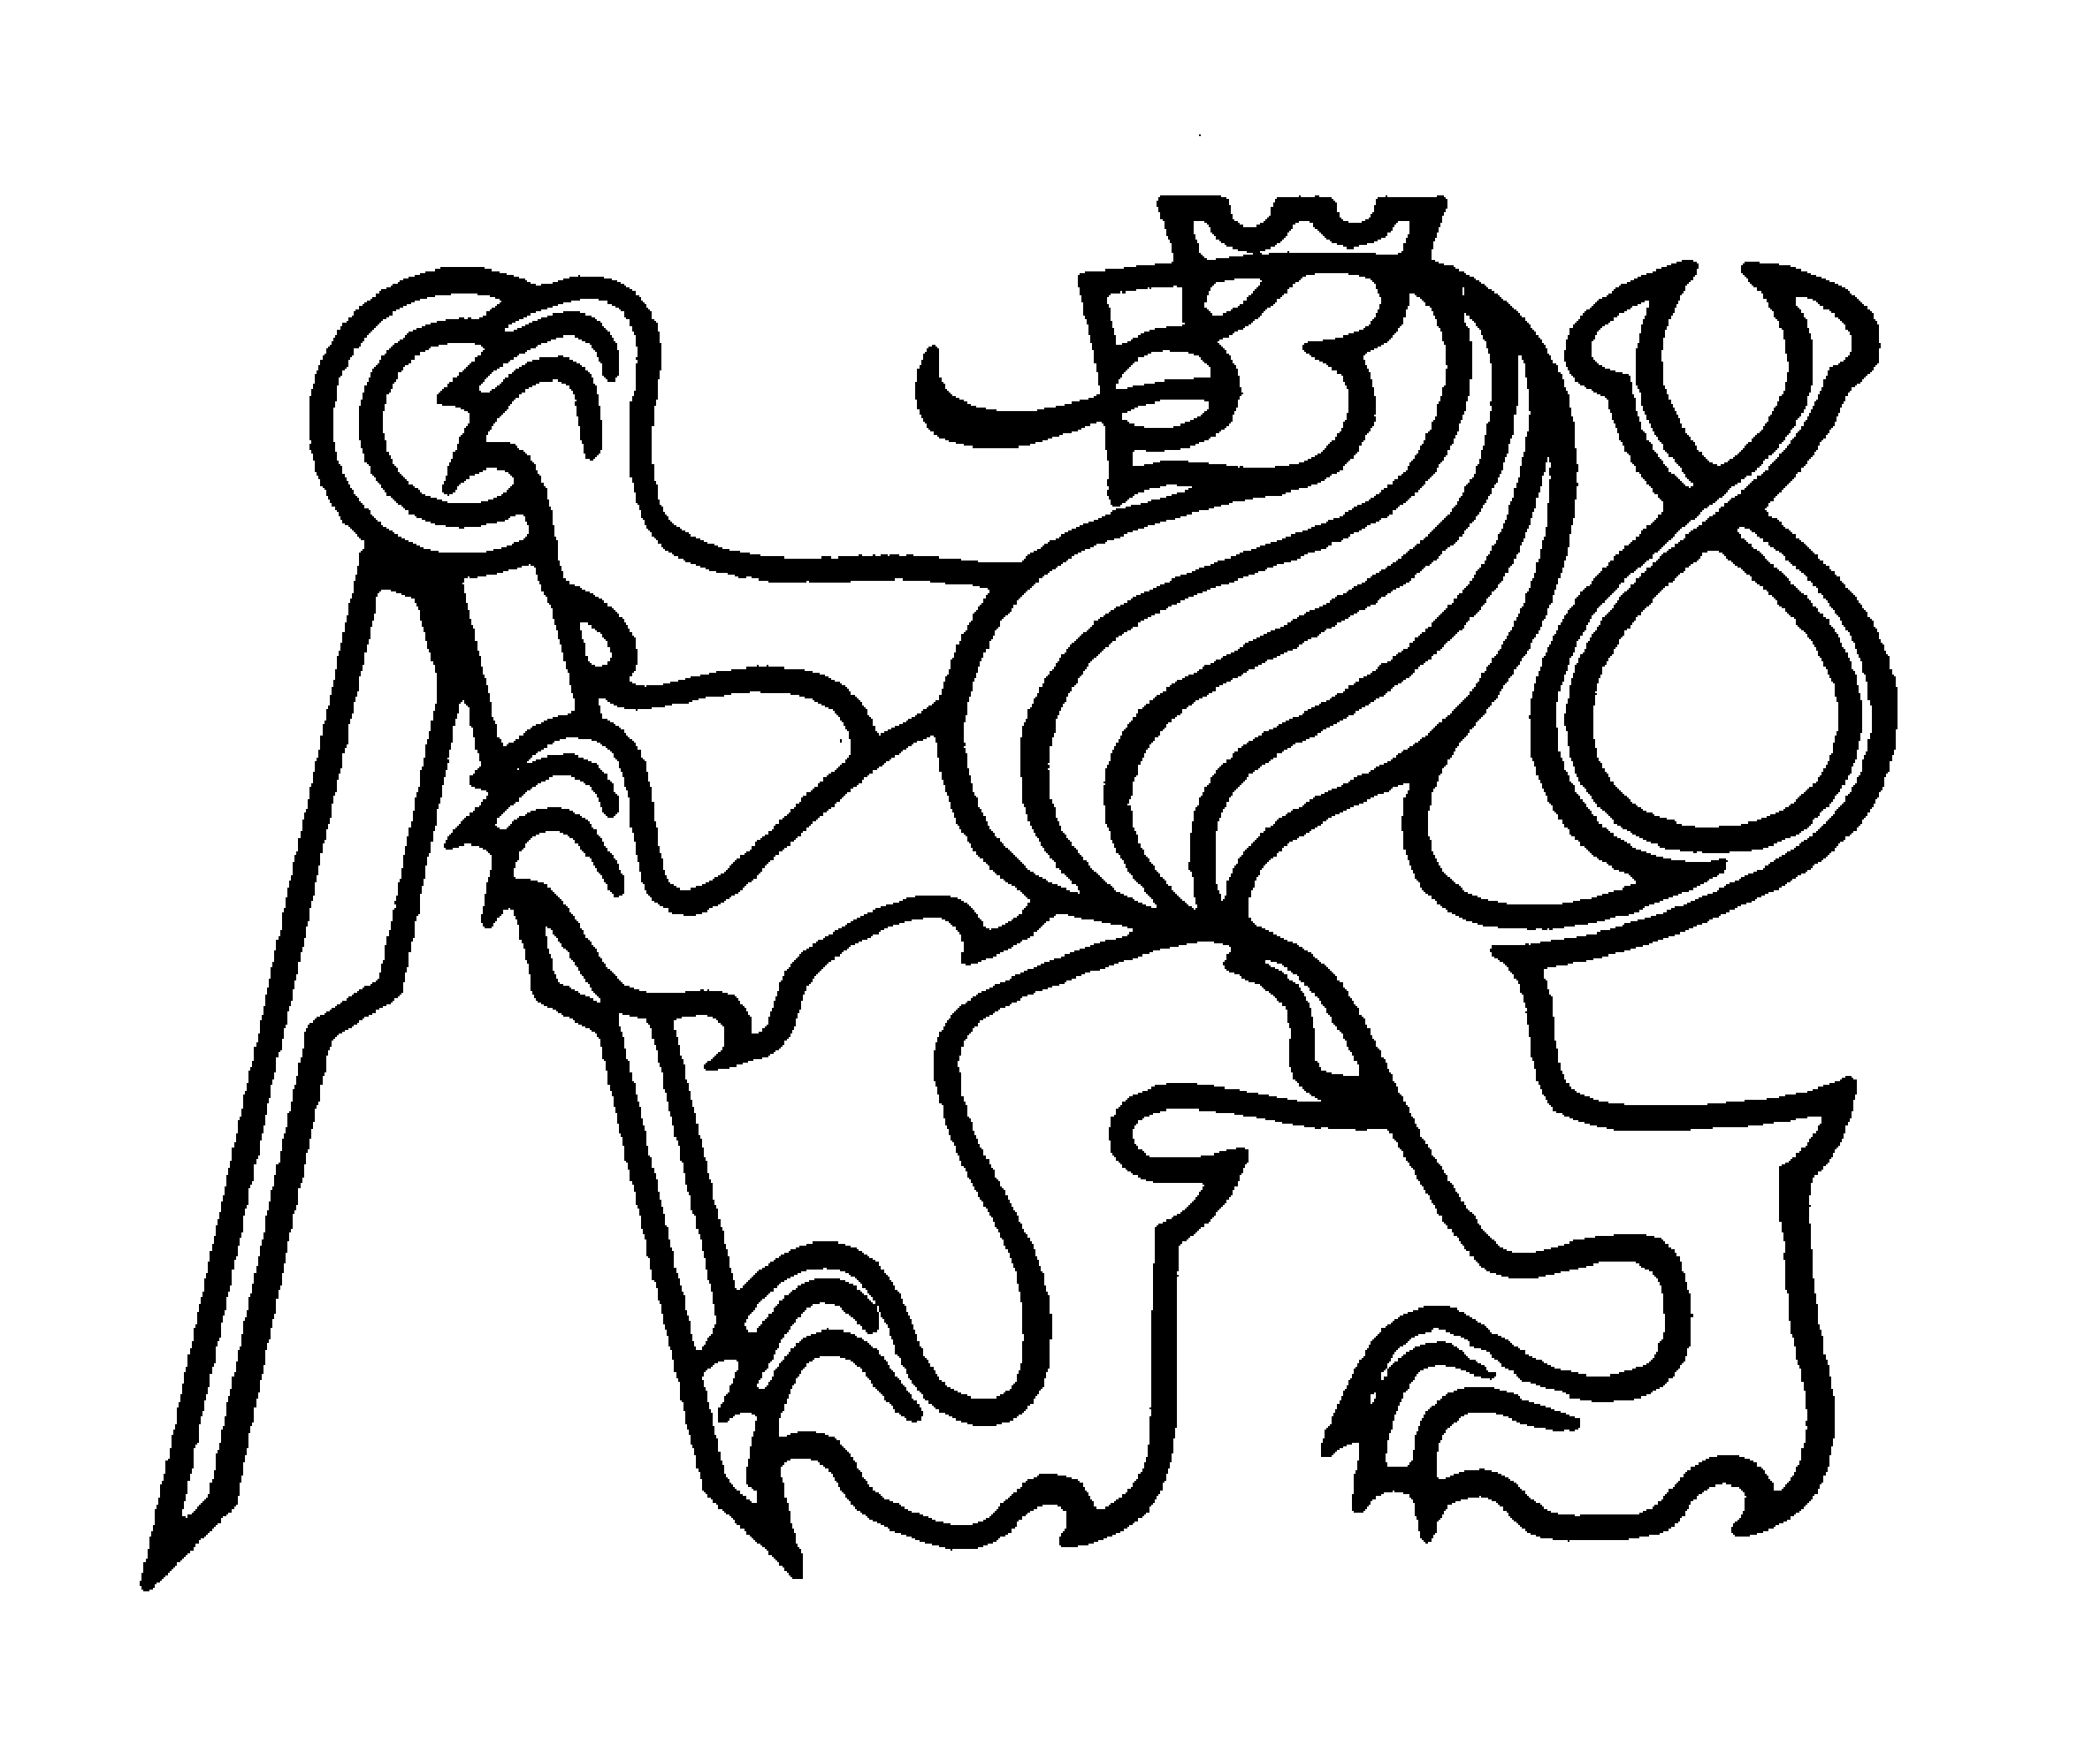
\includegraphics[width=3cm,height=3cm,keepaspectratio]{Images/TITLE/cvut}
\par\end{center}%
\end{minipage}%
\begin{minipage}[c]{0.6\linewidth}%
\begin{center}
\textsc{\large{}Czech Technical University in Prague}{\large{}}\\
{\large{}Faculty of Nuclear Sciences and Physical Engineering}
\par\end{center}%
\end{minipage}%
\begin{minipage}[c]{3cm}%
\noindent \begin{center}
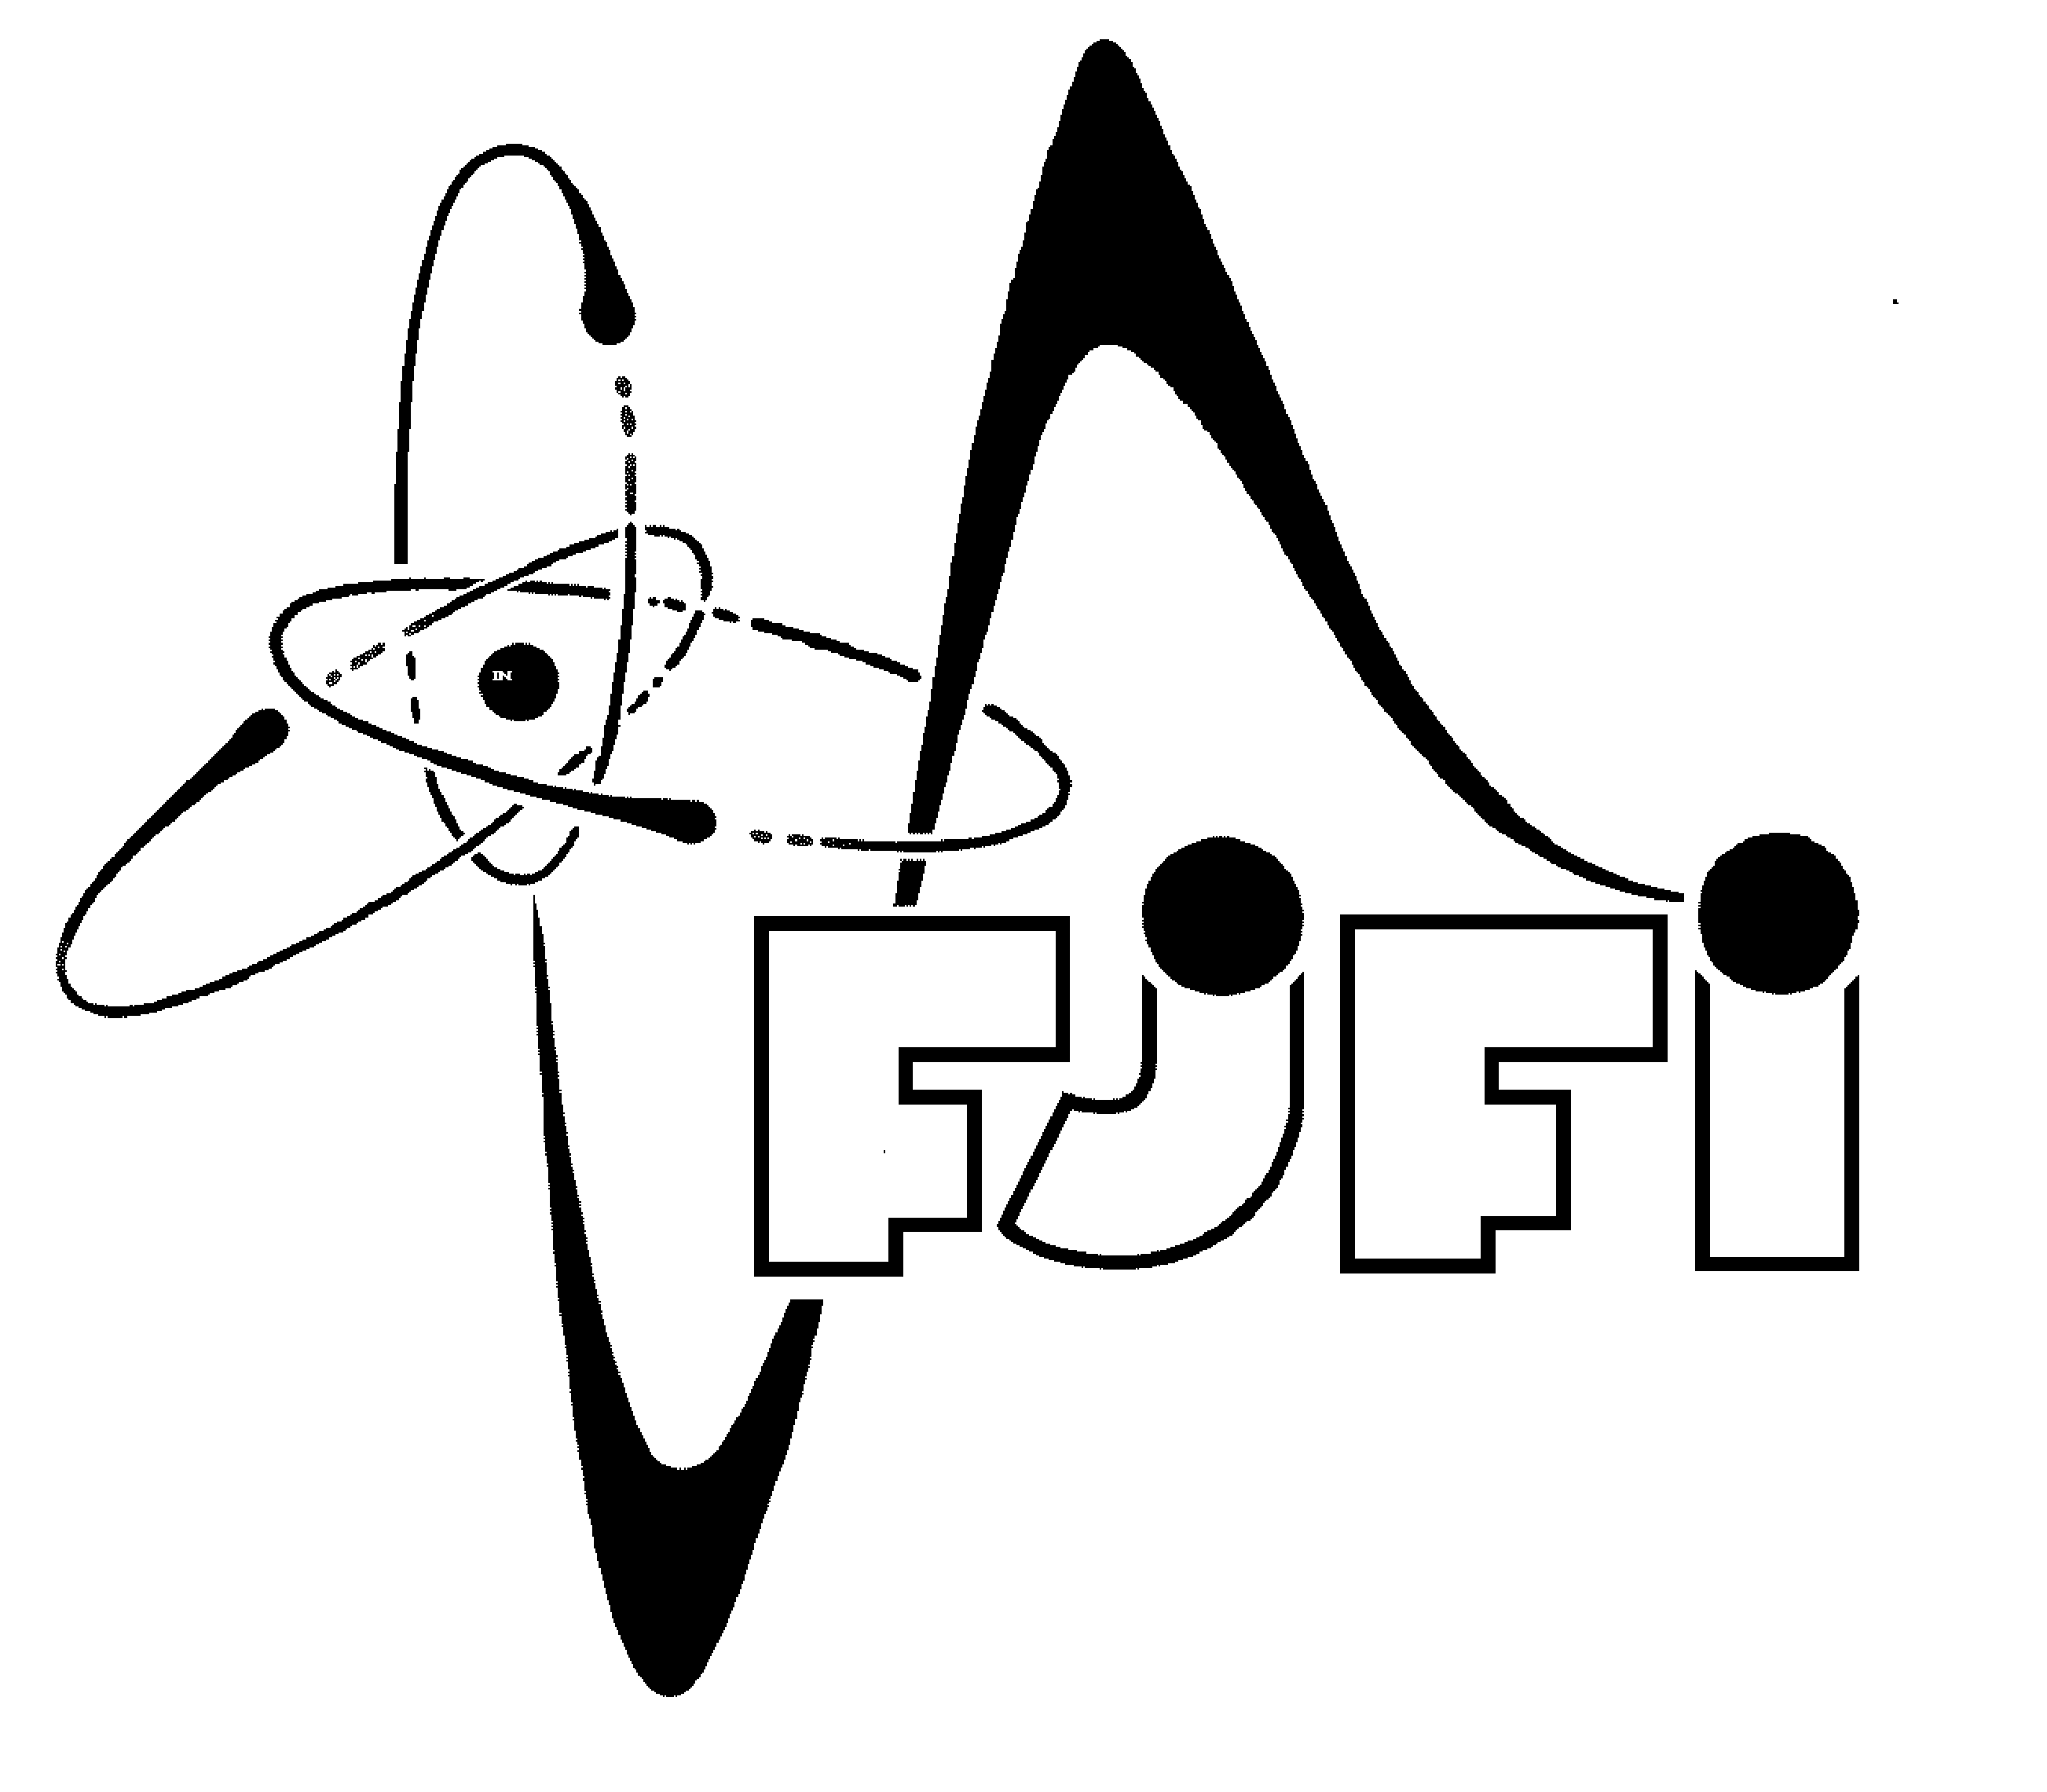
\includegraphics[width=3cm,height=3cm,keepaspectratio]{Images/TITLE/fjfi}
\par\end{center}%
\end{minipage}

\vspace{3cm}

\textbf{\huge{}High performance computing methods for numerical solution of problems with phase transitions}{\huge\par}

\vspace{1cm}

\selectlanguage{czech}%
\textbf{\huge{}Metody vysoce výkonného počítání pro numerické řešení úloh s fázovými přechody}{\huge\par}

\selectlanguage{american}%
\vspace{2cm}

{\large{}Bachelor's Degree Project}{\large\par}

}

\vfill{}

\begin{lyxlist}{MMMMMMMMM}
\begin{singlespace}
\item [{Author:}] \textbf{Kryštof Jakůbek}
\item [{Supervisor:}] \textbf{Ing. Pavel Strachota, Ph.D.}
% \item [{Consultant:}] \textbf{doc. RNDr. Jméno Konzultanta, CSc. }(pouzepokud konzultant byl jmenován.)
\end{singlespace}
% \item [{Language~advisor:}] \textbf{Copeland, Darren, MSc.}
\begin{singlespace}
\item [{Academic~year:}] 2023/2024
\end{singlespace}
\end{lyxlist}

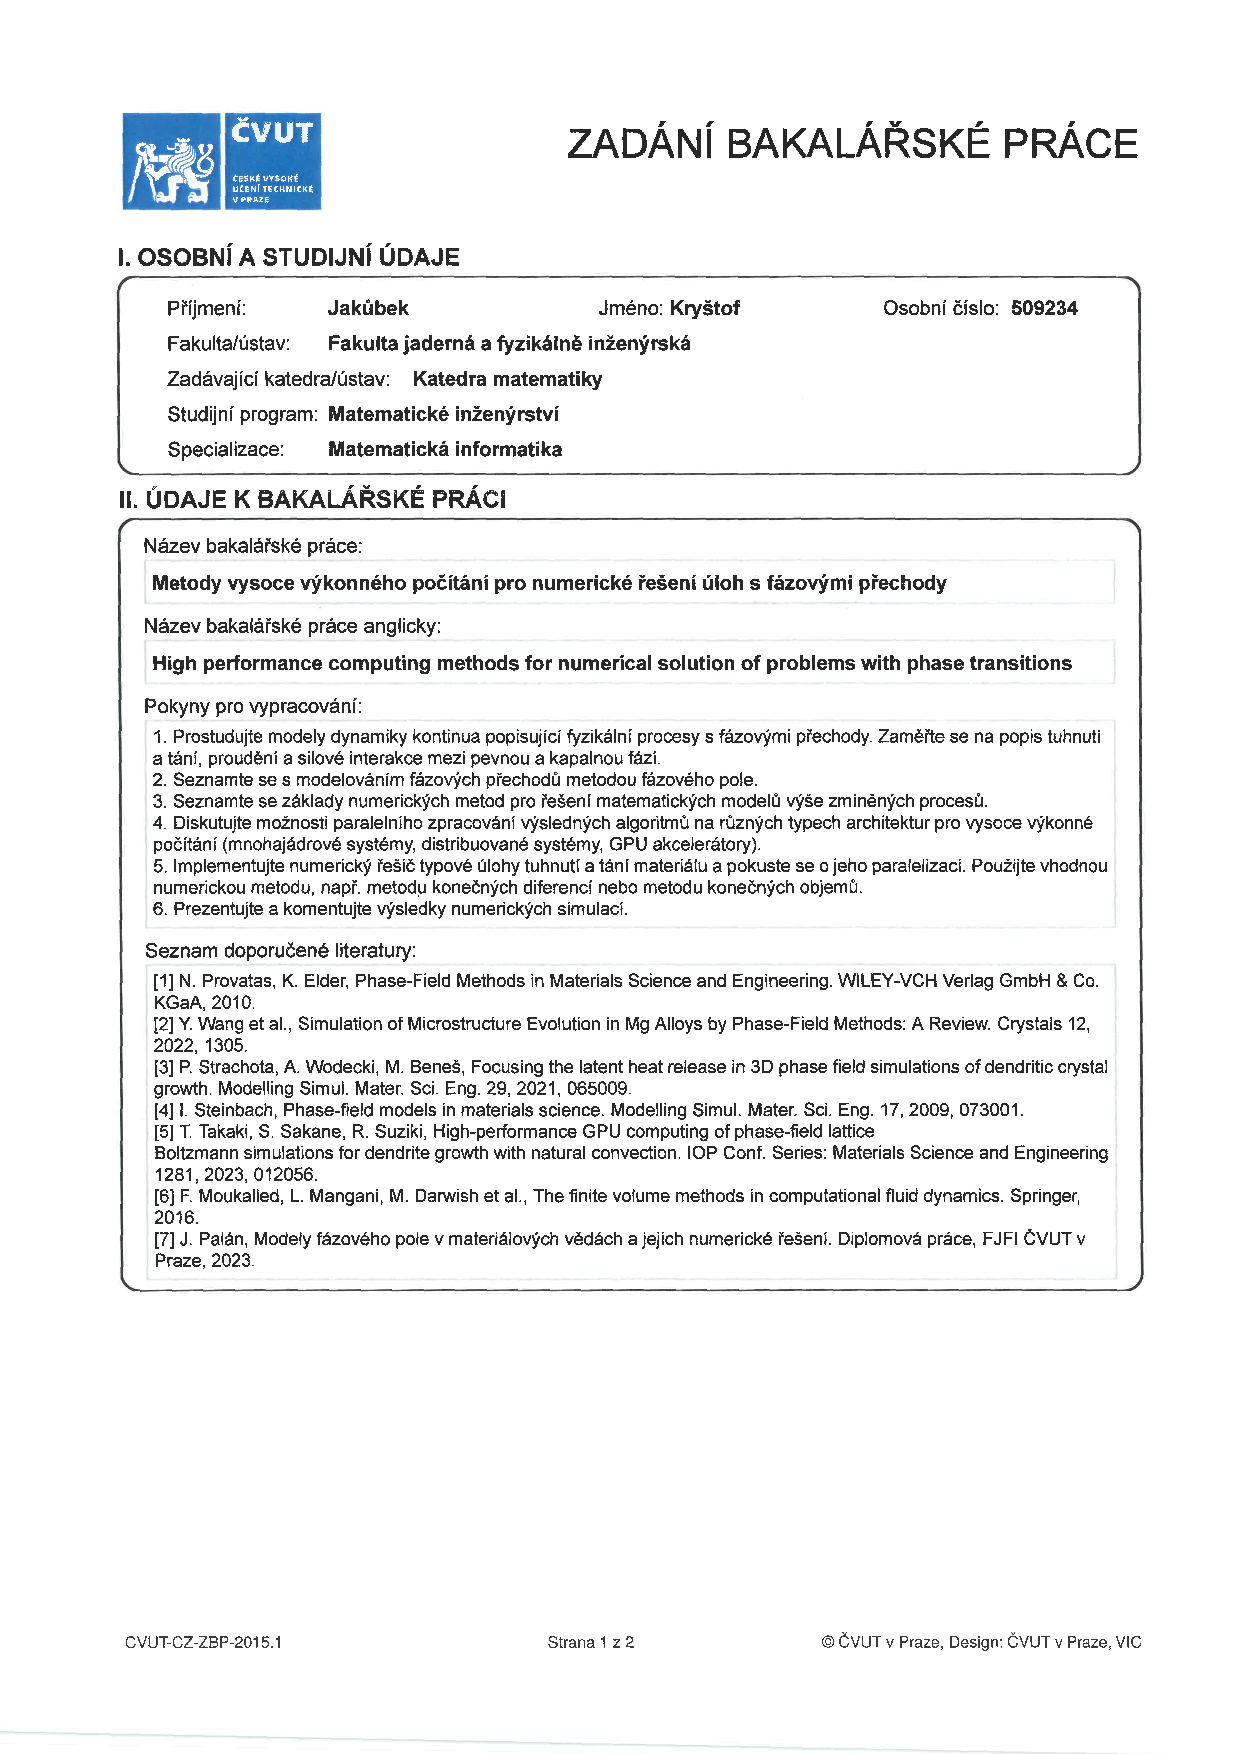
\includepdf[pages=-]{zadani.pdf} 

\noindent \emph{\Large{}Acknowledgment:}{\Large\par}

\noindent I would like to thank my supervisor Ing. Pavel Strachota, Ph.D. for his invaluable insight, critique and seemingly boundless patience. 

\vfill

\noindent \emph{\Large{}Author's declaration:}{\Large\par}

\noindent I declare that this Bachelor's Degree Project is entirely
my own work and I have listed all the used sources in the bibliography.

\bigskip{}

\noindent Prague, \documentdate\hfill{}Kryštof Jakůbek

\vspace{2cm}

\newpage{}

\selectlanguage{czech}%
\begin{onehalfspace}
\noindent \emph{Název práce:}

\noindent \textbf{Metody vysoce výkonného počítání pro numerické řešení úloh s fázovými přechody}
\end{onehalfspace}

\bigskip{}

\noindent \emph{Autor:} Kryštof Jakůbek

\bigskip{}

\noindent \emph{Specializace:} Matematické inženýrství

\bigskip{}

\noindent \emph{Specializace:} Matematická informatika

\bigskip{}

\noindent \emph{Druh práce:} Bakalářská práce

\bigskip{}

\noindent \emph{Vedoucí práce:} Ing. Pavel Strachota, Ph.D.,
Fakulta jaderná a fyzikálně inženýrská, Katedra matematiky

\bigskip{}

% \noindent \emph{Konzultant:} doc. RNDr. Jméno Konzultanta, CSc., pracoviště konzultanta. Pouze pokud konzultant byl jmenován.

\bigskip{}

\noindent \emph{Abstrakt:} Tato práce se zabývá paralelní implementací na GPU numerických schémat pro řešení dvourozměrného modelu fázového pole, popisujícího růst krystalů v podchlazené kapalné fázi. Nejprve je představen model fázového pole. Metoda konečných objemů je využita k odvození semi-diskrétního schématu pro přípustné sítě. Toto schéma je numericky integrováno pomocí explicitních metod vyššího řádu. Poté je odvozeno semiimplicitní schéma časové integrace pomocí Crank-Nicolsonovy metody, které je řešeno pomocí metody konjugovaných gradientů. Dva přístupy ke snížení chyby způsobené použitou metodou štěpení operátorů jsou prezentovány a později porovnány. Je důkladně představeno programování pomocí CUDA a je uvedeno několik simulací využitých optimalizovaných algoritmů. V testu je ukázána efektivita jednoho z popsaných algoritmů. Nakonec jsou porovnány výsledky simulací navržených schémat časové integrace a je ukázána schoda s dřívejšími výsledky.

\bigskip{}

\noindent \emph{Klíčová slova:} CUDA, krystalizace, metoda fázového pole, metoda konečných objemů, paralélní výpočty

\selectlanguage{american}%
\vfill{}

\begin{onehalfspace}
\noindent \emph{Title:}

\noindent \textbf{High performance computing methods for numerical solution of problems with phase transitions}
\end{onehalfspace}

\bigskip{}

\noindent \emph{Author:} Kryštof Jakůbek

\bigskip{}

\noindent \emph{Abstract:} 
This work is concerned with GPU parallel implementation of numerical schemes of the two dimensional phase field model, describing crystal growth in undercooled media. Firstly, the phase field model is introduced and the finite volume method is utilized to derive a semi-discrete scheme for admissible meshes. This scheme is numerically integrated using higher order explicit methods. Then, a semi-implicit time integration scheme is derived using the Crank-Nicolson method and solved using the conjugate gradient method. Two approaches to reduce the error introduced by the operator splitting method are presented and later compared. Programming with CUDA is thoroughly introduced and several optimized algorithms required by the simulation implementation are explained. The efficiency of one of the described algorithms is shown in a benchmark. Finally, simulation results of the proposed time integration schemes are compared and good agreement with previous results is shown. 
\bigskip{}

\noindent \emph{Key words:} CUDA, crystal growth, finite volume method, parallel processing, phase field model

\newpage{}

\pagestyle{plain}

\tableofcontents{}

\newpage{}

\section*{Summary of Notation}
    {
    \setstretch{1.8}
    \begin{tabular}{@{\indent }ll}
        $\Omega$ & Computational domain \\
        $\Timeint$ & Time interval \\
        $\Phi$ & Phase field \\
        $T$ & Temperature field \\
        $a, b, \alpha, \beta, \xi, L, T^*$ & Model parameters  \\
        $\Cells$ & Set of finite volume cells over the domain $\Omega$ \\
        $C, D$ & Grid cells \\
        $\partial C$ & Boundary of grid cell $C$ \\
        $\sigma = C|D$ & Cell face between cells $C$ and $D$  \\
        $m(C)$, $\Tilde{m}(\sigma)$ & Lebesgue measure of cell $C$ and cell face $\sigma$ \\
        $\rho(x, y)$ & Distance between points $x$ and $y$ \\
        $\rho(x, \sigma) = \halfinf{y \in \sigma}{\rho(x,y)}$ & Distance between point $x$ and cell face $ \sigma$ \\
        $\vec{x}_C$ & Position in the centroid of cell $C$ \\
        $E, W, N, S$ & Cells to the East, West, North and South relative to cell $C$, respectively \\
        $\vec{e}_1, \vec{e}_2, \vec{e}_3$ & Ortonormal basis vectors of $\R^3$ \\
        $\Gamma(t)$ & Approximate shape of the phase interface
    \end{tabular}
    }
% ================================ CONTENT ====================
\chapter*{Introduction}

\addcontentsline{toc}{chapter}{Introduction}

Solidification forms a crucial step in many practical applications including metallurgy, semiconductor manufacturing and optics. The microscopic crystal structure of the resulting material can have profound impact on its mechanical, electric and magnetic properties. Because of this, simulating the crystal structures ahead of time can be of interest. Goal of this work is to derive and efficiently implement a numerical scheme for solving the phase field problem, governing solidification of undercooled media and dendritic crystal growth. While other methods have been proposed and implemented with excellent scaling properties on many core setups \cite{Starchota2016Implementation}, \cite{J.Palan}, they are limited to the CPU. Thus, to achieve fast simulation running times, access to specialized high performance computing cluster is required. We present a numerical scheme and its implementation capable of achieving good runtime on consumer hardware. For this purpose the implementation has been devised to run efficiently on the GPU, which provides excellent compute capabilities for massively parallel workloads encountered in the simulation.

This work is divided into five chapters. Chapter \ref{chap:mat analisis} provides an overview of the models of solidification in undercooled media, which will be utilized in the rest of the text. For this Stefan and phase field problems are introduced. Models of fluid flow incorporating the interaction between fluid and solid particles are briefly reported on.

The Chapter \ref{chap:fvm} is focused on the finite volume method. The general finite volume framework is introduced and then utilized to derive the discretization of the gradient and Laplacian operators. Then, common boundary conditions are described within the finite volume framework. Lastly, the phase field model described in Chapter \ref{chap:mat analisis} is discretized into the so-called semi-discrete scheme.

The Chapter \ref{chap:time integration schemes}, is concerned with the derivation of time integration schemes for the semi-discrete scheme from Chapter \ref{chap:fvm}. Two categories of schemes are derived. First category are the explicit schemes, which solve the semi-discrete scheme by direct calculation. Second category are the semi-implicit schemes, which reformulate the problem into a system of linear equations and solve it using an appropriate matrix solver. The error caused by approximations done during the time integration scheme derivation is quantified and two approaches for reducing this error are presented.

The Chapter \ref{chap:Implementation} thoroughly introduces programming on the GPU utilizing the CUDA programming model. It details several optimized algorithms used during the implementation of schemes derived in Chapter \ref{chap:time integration schemes}. A special effort was put on the explanation in hopes that even an unfamiliar reader may understand the algorithms presented. It showcases the efficiency of one of the presented algorithms by comparing it with the CUDA Thrust library.

The Chapter \ref{chap:results} presents and discusses the results obtained by running the developed simulation. Effect of various model parameters as well as boundary conditions is shown. Then the schemes proposed in Chapter \ref{chap:time integration schemes} are compared and the impact of the described error reduction approaches presented is evaluated.

\chapter{Mathematical modeling of phase transitions}\label{chap:mat analisis}
\pagestyle{headings}

Solidification is a phase transition of the first order occurring mainly as a result of temperature change. However, solidification of undercooled liquid only occurs upon a slight energy disturbance, typically caused by impurities in the liquid around which an initial nucleus of solid phase is formed. This initial nucleus then interacts with its surroundings, causing it to solidify as well, resulting in crystal growth. The changing shape of the solid region combined with different conditions in each of the material phases poses a unique modeling challenge. For this, two approaches of modeling solidification were developed: the first ones are the sharp interface models, which explicitly track the position of the interface between the solid and liquid phases \cite{Schmidt1996Exact}. The second ones are the phase field models, sometimes also called smooth interface models, which utilize a scalar field to represent the phase of the material in the specific point in time and space. A rapid but smooth transition between the phases is assumed \cite{Raabe1998}.

The phase field approach has been successfully used to simulate, amongst others dendritic growth in pure supercooled melts \cite{Wheeler93Dendrites}, in binary alloys \cite{Wheeler92BinaryAlloys} and in interaction with fluid flows \cite{Bajo2022FSI}.

This text will focus on solidification of pure undercooled substances in two dimensions utilizing the phase field model, still, a general introduction is given.  
We first introduce the Stefan problem with surface tension, which is a sharp interface model, then present its corresponding phase field formulation, which will be studied further. Finally, we report on the models of hydro-mechanical phenomena. 

\newpage
\section{The Stefan problem} \label{sec:Stefan problem}
    Consider domain $\Omega \subset \R^3$ alongside time interval $\Timeint = [t_\text{begin}, t_\text{end}]$. At each $t \in \Timeint$ the domain $\Omega$ is divided into a solid subdomain $\Omega_s(t)$ and a liquid subdomain $\Omega_l(t) = \Omega \setminus \Omega_s(t)$, separated by a phase interface $\Gamma(t) = \partial \Omega_s(t) \cap \partial \Omega_l(t)$. The Stefan problem \cite{BenesSolidification2001} is given as 
    \begin{align}
        \rho c \dert{T} = \nabla(\lambda\nabla T) && \text{ in } \Timeint \times \Omega_s(t) \text{ and } \Timeint \times \Omega_l(t), \label{eq:stefan heat} \\ 
        b_c(u)|_{\partial\Omega} = 0 && \text{ on } \Timeint \times \Omega, \label{eq:gibbs-thomas condition} \\
        T|_{t=0} = T_{ini} && \text{ in } \Omega, \\
        \lambda \frac{\partial T}{\partial \vec{n}_\Gamma}\bigg\rvert_{s} - \lambda\frac{\partial T}{\partial \vec{n}_\Gamma}\bigg\rvert_{l} = L\nu_\Gamma && \text{ on } \Gamma(t), \label{eq:stefan condition} \\
        T - T^* = -\frac{\sigma}{\Delta s} \kappa_\Gamma - \alpha\frac{\sigma}{\Delta s}\nu_\Gamma && \text{ on } \Gamma(t), \\
        \Omega_s(0) = \Omega_{s, ini}, \label{eq:stefan last}
    \end{align}
    where the $T:\Timeint\cross\Omega \to \R$ is temperature field. The model parameters $\rho, c, \lambda, L, u*, \sigma, \Delta s, \alpha \in \R$ alongside $\vec{n}_\Gamma \in \R^3, \nu_\Gamma, \kappa_\Gamma \in \R$ are described in Table \ref{tab:Stefan problem params}. 
    In the Stefan problem, (\ref{eq:stefan heat}) is the heat equation, evaluated separately in the liquid and solid subdomains, (\ref{eq:gibbs-thomas condition}) is the Gibbs-Thomson relation and (\ref{eq:stefan condition}) is the Stefan condition, describing heat flow discontinuity at the phase interface $\Gamma$. 
    $\vec{n}_\Gamma$ is the normal vector to $\Gamma(t)$, 
    $b_c$ is the boundary condition operator which can be taken as 
    \begin{align*}
        b_c(T) &= T - T^* && \text{ for the Dirichlet boundary condition or} \\
        b_c(T) &= (\lambda\nabla T - \vec{g}) \cdot \vec{n}_{\partial \Omega} && \text{ for the Neumann boundary condition}, 
    \end{align*}
    where vector $\vec{g}$ specifies heat flux through $\partial \Omega$ and $\vec{n}_{\partial \Omega}$ is the normal to $\partial \Omega$ in the given point.

\FloatBarrier
\begin{table}[!ht]
    \centering
    \begin{tabular}{|ll|ll|}
        \hline 
         $\rho$ & material density                        & $T^*$      & material melting point \\
         $\lambda$ & heat conductivity                    & $\Delta s$ & difference in entropy per unit volume \\
         $L$ & latent heat of fusion per unit volume      & $\alpha$   & coefficient of attachment kinetics \\
         $\nu_\Gamma$  & normal velocity of $\Gamma(t)$   & $\sigma$   & surface tension \\ 
         $\vec{n}_\Gamma$ & normal vector to $\Gamma(t)$  & $c$        & material specific heat capacity \\
         $\kappa_\Gamma$ & mean curvature of $\Gamma(t)$  & & \\
        \hline
    \end{tabular}
    \caption{Parameters of the the Stefan problem}
    \label{tab:Stefan problem params}
\end{table}
\FloatBarrier

\section{Phase field problem} \label{sec:phase field model}
    We transition from the Stefan problem (\ref{eq:stefan heat}) - (\ref{eq:stefan last}) to its phase field formulation. We consider the phase field $\Phi:\Timeint \times\Omega \to [0, 1]$, which represents phase of the material in the given point in time $t \in \Timeint$ and space $\vec{x} \in \Omega$. Points where $\Phi(t, \vec{x}) < 1/2$ are considered liquid and points where $\Phi(t, \vec{x}) \ge 1/2$ are consider solid. Specifically the phase interface $\Gamma(t)$ is defined as 
    \begin{align*}
        \Gamma(t) = \left\{ \vec{x} \in \Omega, \Phi(t, \vec{x}) = \frac{1}{2} \right\},
    \end{align*}
    which lets us to represent $\vec{n}_\Gamma$, $\nu_\Gamma$ and $\kappa_\Gamma$ as
    \begin{align}
        \vec{n}_\Gamma = - \frac{\nabla \Phi}{\abs{\nabla \Phi}}, 
        && \nu_\Gamma = \frac{1}{\abs{\nabla \Phi}}\dert{\Phi}, 
        && \kappa_\Gamma = \nabla \cdot \vec{n}_\Gamma.
    \end{align}
    The phase field problem given by \cite{BenesSolidification2001} reads 
    \begin{align}
        \dert{T} &= \laplace{T} + L\dert{\Phi}                                                &&\text{ in } \Timeint\times\Domain, \label{eq: Phase field original T equation} \\
        \xi^2\alpha\dert{\Phi} &= \xi^2\laplace{\Phi} + f(\Phi, T, \nabla \Phi) \label{eq: Phase field original Phi equation}              &&\text{ in } \Timeint\times\Domain, \\
        T|_{t=0} &= T_{ini}                                                                     &&\text{ in } \Omega, \\ 
        \Phi|_{t=0} &= \Phi_{ini}                                                               &&\text{ in } \Omega, \\
        T|_{\partial \Domain} &= T_{\partial \Domain} \text{ or } \nabla{T}\cdot\vec{n} = 0            &&\text{ in } \Timeint\times\partial\Domain, \\
        \Phi|_{\partial \Domain} &= \Phi_{\partial \Domain} \text{ or } \nabla{\Phi}\cdot\vec{n} = 0   &&\text{ in } \Timeint\times\partial\Domain, 
    \end{align}
    where $L, \alpha, \beta$ are dimensionless forms of the original parameters of the Stefan problem (\ref{eq:stefan heat}) - (\ref{eq:stefan last}). They are calculated as
    \begin{align*}
        L = \bigfrac{L_\text{real}}{\rho c\Delta T_{ini}}, 
        && \alpha = \alpha_\text{real} \bigfrac{\lambda}{\rho c}, 
        && \beta = \bigfrac{\Delta s}{\sigma}L_0\Delta T_{ini},  
    \end{align*} where we used $L_\text{real}$, $\alpha_\text{real}$ to refer to the original parameters in Section \ref{sec:Stefan problem}. $\Delta T_{ini} = T_{ini} - T^*$ is the uniform initial undercooling, $t_0$ is the time scale and $L_0 = \sqrt{\frac{\lambda}{\rho c}t_0}$ is the length scale. 
    
    In (\ref{eq: Phase field original Phi equation}), $f(\Phi, T, \nabla \Phi)$ is the so-called reaction term. Multiple forms of the reaction term have been proposed with distinct physical and numerical properties \cite{Caginalp1989}, \cite{Kobayashi1993}, \cite{Strachota_dendric_crystal}. We will use the form given in \cite{BenesSolidification2001}, which is written as
    \begin{align}
        f(\Phi, T, \nabla \Phi) &= af_0(\Phi) - b\xi^2\beta\abs{\nabla \Phi}(T - T^*) \label{eq:reaction term}, \\
        f_0(\Phi) &= \Phi(1-\Phi)(\Phi - \frac{1}{2}). 
    \end{align}
    Lastly, the parameter $\xi > 0$ controls the width of the phase transition. It has been shown that given certain conditions, the solution to the phase field problem converges to the solution of the original Stefan problem with $\xi \to 0_+$ \cite{Benes1997Dizertace}. 
    
\FloatBarrier
    \begin{figure}[!ht]
        \centering
        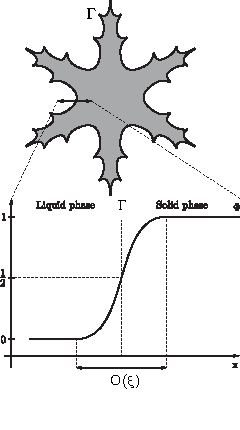
\includegraphics[height=12cm]{diagrams/diffuse_interface_2.pdf}
        \caption{Phase field $\Phi$, phase interface $\Gamma$ and the shape of phase transition, whose width is proportional to $\xi$}
        \label{fig:phase interface}
    \end{figure}
\FloatBarrier

    The characteristic shape of the phase transition is depicted in Figure \ref{fig:phase interface}. The shape is the result of $f_0(\Phi) = \bigfrac{\dd \omega_0(\Phi)}{\dd \Phi}$, where $\omega_0$  is the bulk free-energy density, defined as $\omega_0(\Phi)~=~a\Phi^2(1 - \Phi)^2/4$ \cite{Caginalp1989}. The two local minima of $\omega_0$ in values 0 and 1, corresponding to the liquid phase and solid phase respectively, are shown in Figure \ref{fig:double well}.
    
\FloatBarrier
    \begin{figure}[!ht]
        \centering
        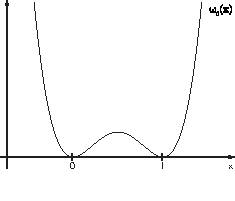
\includegraphics[height=5cm]{diagrams/double_well.pdf}
        \caption{the double well potential $\omega_0$}
        \label{fig:double well}
    \end{figure}
\FloatBarrier
    
    \subsection{Anisotropy}
    The phase field model described in Section \ref{sec:phase field model} is not sufficient to generate the complex crystal structures found in nature. One common characteristic of such structures is anisotropy, that is, stronger tendency of the crystal to grow in certain directions compared to others. Models of anisotropy utilizing the concept of surface motion and Finsler geometry have been proposed and successfully implemented \cite{Benes2003CurvatureFlow}, \cite{Belletini1996FinslerGeo}, \cite{StrachotaDizertation}. However, for simplicity, we will use the two dimensional model given in \cite{Benes2001MatAnalysis}
    \begin{align}
    \xi^2\alpha\dert{\Phi} &= g(\theta)\xi^2\laplace{\Phi} + g(\theta)af_0(\Phi) - b\xi^2\beta\abs{\nabla \Phi}(T - T^*), \label{eq: Anisotropy definition} \\
    g(\theta) &:= 1 - S\cos(m(\theta_0 - \theta)),  
    \end{align}
    where $\theta \in \R$ denotes the angle between the phase interface normal and the basis vector $\vec{e}_1$, $S \in [0, 1)$ is strength of $m$-fold anisotropy and $\theta_0 \in \R$ is principal crystallographic orientation \cite{BenesSolidification2001}. Note that $\theta$ can be computed using 
    \begin{align}
        \theta = \text{atan2}(\der{\Phi}{y}, \der{\Phi}{x}).
    \end{align}
    
    \FloatBarrier
    \begin{figure}[!ht]
        \centering
        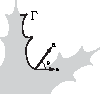
\includegraphics[height=5.4cm]{diagrams/aniso_normal_2.pdf}
        \caption{
            Angle $\theta$ between the phase interface normal $\vec{n}$ and basis vector $\vec{e}_1$
        }
        \label{fig:aniso normal}
    \end{figure}
    \FloatBarrier

    To simplify notation in the upcoming sections we will rewrite the phase field problem equations (\ref{eq: Anisotropy definition}), (\ref{eq: Phase field original T equation}) using nonlinear functions $k1, k2, k3$ 
    \begin{align*}
        \dert{\Phi} &= 
              \underbrace{\frac{g(\theta)}{\alpha}}_{k_1(\nabla\Phi)}\laplace{\Phi} 
            + \underbrace{\frac{g(\theta)af_0(\Phi)}{\xi^2\alpha}}_{k_0(\nabla\Phi)} 
            + \underbrace{\frac{b\beta\abs{\nabla \Phi}}{\alpha}}_{k_2(\nabla\Phi)}(T^* - T), 
    \end{align*}
    as
    \begin{align}
        \dert{T} &= \laplace{T} + L\dert{\Phi}, \label{Allen-Cahn kform T}\\
        \dert{\Phi} &= k_1(\nabla\Phi)\laplace{\Phi} + k_0(\Phi, \nabla\Phi) + k_2(\nabla\Phi)(T^* - T) \label{Allen-Cahn kform Phi}.
    \end{align}
    This formulation will be used in the remainder of the text.

    \section{Hydro-mechanical phenomena}
	In this section, we report on models describing fluid-structure interaction (FSI). This exploration was motivated by modeling of freezing water in porous media, where under certain conditions, mechanical effects can be very significant. First, we summarize various approaches to FSI and describe in detail, the method presented in \cite{Reder2021}. Second, we focus on poromechanical interactions of freezing water and describe the model given in \cite{ZakBenes2023}, \cite{ZakBenes2018}.  
 

    \subsection{Fluid structure interaction}

	Two broad categories for modeling FSI are used. One category of approaches are the body-fitted mesh methods, such as the arbitrary Lagrange-Euler method \cite{Johnson1996}. The simulation grid is dynamically adjusted to the movement of the solids, while ensuring the grid nodes are located at the solid-liquid interface. For significant changes to the grid, for example caused by the solid's rotation, the grid needs to be remeshed, which incurs high computational cost and errors resulting from interpolation of fields into the new grid \cite{Basting2017ALE}, \cite{Bajo2022FSI}. Another option is the immersed boundary method (IBM) \cite{Peskin1972IBM}, which solves the Navier-Stokes equations, while accounting for interactions with one dimensional fibers described in Lagrangian coordinates.

	The second category is based entirely on Eulerian description of both liquids and solids.
	% D. Anderson, G. McFadden, and A. Wheeler. A phase-field model of solidification with convection. Physica D, 135:175-194, 2000
	One such approach is to model the solids as extremely high viscosity Newtonian fluids and solve the standard Navier-Stokes equations \cite{Anderson2000FSI}. This approach is conceptually simple, but suffers from poor numerical performance and does not represent the constitutive behaviour of solids \cite{Vieyra2005Masters}.
	Next, \cite{Tong2001Convection}, \cite{Beckermann2001} investigate the effects of convection on dendritic crystal growth in the phase field model. However, the growing particles are kept stationary, thus the full extent of FSI is not modeled. Another set of methods are the distributed Lagrange multiplier methods (DLM) on a fictious domain, which enforced rigid body motion for the solid via a field of Lagrange multipliers. Examples of this method include \cite{Gallier2014}, \cite{Reder2021}, which show promising results in modeling the fluid-structure, structure-fluid and structure-structure interactions for large amounts of separate particles of various geometries. A rough description of the model presented in \cite{Reder2021} follows.
   	 
	The DLM method given in \cite{Reder2021} models the interaction between a set of particles and the surrounding incompressible fluid. Both fluid-structure and structure-structure interactions are considered. Each particle is represented using a phase field defined similar to the model given in Section \ref{sec:phase field model}. In total, $N$ phase fields are tracked to represent $N$ bodies.
    
	Fluid-structure interaction is achieved by transport of the phase fields by the fluid flow. The Navier-Stokes equations are solved in the whole domain, without considering the solid particles, represented by the so-called ghost fluid. Then using the resulting velocity field, a barycenter velocity and angular velocity are calculated for each particle. This motion is subsequently reprojected into the velocity field in the region covered by said particle. This results in a near constitutive behavior of the solid particles. Still, some error is committed, thus the Allen-Cahn equation \cite{Allen-Cahn}, governing the shape of the phase field, is solved every couple of time steps. This restores the phase interface into the expected characteristic shape.
    
	Structure-structure interaction is detected by utilizing the smooth transition between phases in the phase-field model. If the value of phase fields for both of the particles is higher than a certain amount and the particles are moving in opposite directions, the particles are considered to be interacting. The interaction is resolved using the particle distance and the calculated barycenter velocities. This procedure is repeated for all contact points in a single time step.

	This model successfully resolves interactions of many spherical particles immersed in a fluid, interaction of spherical particles and static complex mesh as well as simultaneous FSI and grain growth.

    \subsection{Poromechanical interaction}
    Variety of approaches modeling water freezing is porous media have been developed. For some early macroscopic models see \cite{Gilpin1980}, \cite{Fowler1989}. \cite{ZhouMeschke2013},\cite{ZhengXing-Yuan2017} used theory of porous media to derive a fully integrated thermo-hydro-mechanical model able to describe liquid transport within pores, latent heat effect and the deformation of the solid. The remainder of this section will be devoted to describing the models given in \cite{ZakBenes2023} and \cite{ZakBenes2018}. 
    
    The model given in \cite{ZakBenes2023} describes water freezing on a microscopic (pore-scale) level. The geometry of the pores created between arbitrary shaped particles is used directly without any spatial averaging. Because of this, it may provide more accurate results on the micro scale. 
    
    In any given point of the domain there may be water, ice or solid particle. Each of the materials is equipped with momentum and energy conservation equations. Ice and solid particle materials are assumed to be linearly elastic, while water is assumed to be a slightly compressible Newtonian fluid. Next, the materials are linked with each other through equations of heat transfer through their shared boundary. Transfer through the water-ice boundary is modeled using the Stefan condition \ref{eq:stefan condition}.

    The phase field model with anisotropy similar to the model given in Section \ref{sec:phase field model} is employed to describe the motion of the water-ice boundary. Quantities on the smooth water-ice interface are assumed to depend linearly on the value of the phase field in the given point. Expansion of the ice phase is captured with slight modification of the water and ice stress tensor. Finally, boundary conditions for heat fluxes and stress tensors of the materials are given. The phase field is assumed to be liquid at the water/ice-particle boundary, helping the model avoid singularities related to the shared water-ice-particle boundary, while also more closely modeling experimentally observed phenomena. 
    
    Via computational studies the resulting model is shown to be able to describe various structural dynamics of the solid phase within complex solid particle geometries. The ice material is shown to spread and fill in the pore space as well as be transported by the created fluid flow. 
    
    Earlier study by the same authors \cite{ZakBenes2018} has shown the viability of a similar model to describe displacement of the material as a result of ice phase expansion.
    
    % Phase filed for each particle is used to track its position considers $N$ rigid bodies in the domain $\Omega$. These rigid bodies are described using $N$ phase fields $\phi_p:\Timeint\times\Omega \to [0, 1]$ $\forall p \in \hat{N}$, where
    % \begin{align}
    %     \Omega_p = \left\{ \vec{x} \in \Omega, \phi_p(\vec{x}) \ge \frac{1}{2} \right\} && \forall p \in \hat{N}
    % \end{align} 
    % and defines the solid and liquid subdomain as
    % \begin{align}
    %     \Omega_s = \bigcup_{p = 1}^N \Omega_p, && \Omega_l = \Omega \setminus \Omega_s.
    % \end{align}

    % \newcommand{\DD}[0]{\text{D}}

    % The system is described by the momentum balance equation 
    % \begin{align}
    %     \rho \frac{\DD \vec{u}}{\DD t} = \rho \vec{f}_V + \nabla \cdot \vec{\sigma} && \text{ in } \Omega
    % \end{align}
    % with the rigidity constraint
    % \begin{align}
    %     \frac{1}{2}\left(\nabla \vec{u}  + (\nabla \vec{u})^T \right) = \vec{0} && \text{ in } \Omega_s \\
    % \end{align}
    % and continuity equation
    % \begin{align}
    %     \nabla \vec{u} = \vec{0} && \text{ in } \Omega_l,
    % \end{align}
    % where $\vec{u}$ is the velocity field, $\rho$ the mass density, $\vec{f}_v$ the body force and $\vec{\sigma}$ the Cauchy stress tensor. The operator $\frac{\DD}{\DD t} = \dert{} + \vec{u}\cdot \nabla$ is the material derivative and the operator $D(\cdot) = \frac{1}{2}\left(\cdot  + \cdot^T \right)$ is the symmetric part of the tensor. The momentum balance equation is solved in two steps. First, the solid is represented by the so called ghost fluid and the equation is solved with the continuity equation on the whole domain, yielding the Navier-Stokes system 
    % \begin{align}
    %     \rho \frac{\DD \vec{u}}{\DD t} = \rho \vec{f}_V + \nabla \cdot \vec{\sigma} && \text{ in } \Omega,
    %     \nabla \vec{u} = \vec{0} && \text{ in } \Omega_l,
    % \end{align}
    % where Newtonian fluid with dynamic viscosity $\mu$ was assumed. This produces correct solution $\vec{u}^*$ of the velocity field in the liquid subdomain and preliminary velocity field in the solid subdomain. Then the 
    
    
    
\chapter{Finite volume method}\label{chap:fvm}
    Since analytical solution of the phase field problem given in Section \ref{sec:phase field model} is not known, we attempt to obtain a numerical solution. The first step towards numerical solution of a parabolic PDEs is spatial discretization, for which we choose the finite volume method (FVM). 

    The FVM is a discretization method broadly used in simulations of fluid dynamics, heat and material transfer problems \cite{Blazek2015FVM}. The FVM divides the computational domain into a finite number of regions of polygonal or polyhedral shape called \emph{elements} or \emph{cells}. Then the studied partial differential equation are integrated over each of the elements, yielding a discretized system of algebraic equations, which are then solved to compute the values of the dependent variables \cite{MoukalledFVM2016}. 

    Because fluxes are shared between the neighbouring elements, that is a flux entering an element is equal the flux leaving its neighbour, the FVM is locally conservative. This makes it a good fit for discretizing conservation laws \cite{MoukalledFVM2016}.

    Another advantage of the FVM is its versatility with regards to the structure and geometry of the cells used, the so called mesh. Meshes can be broadly classified into \emph{structured} and \emph{unstructured}. Cells in a structured mesh are specified in well defined order, for example in a grid of uniformly sized rectangular or triangular cells. Cells in unstructured meshes are in generally arbitrary order, only defined by connectivity. This allows for simulation of problems on complex geometries.

    We introduce the formalism of finite volume meshes, derive the spatial discretization of Laplacian and gradient operators on a simple structured mesh, implement boundary conditions using ghost cells, and finally formulate a semi-discrete scheme of the phase field model.
    
    \section{General mesh} \label{sec:general mesh}
    
    Let $\Omega$ denote an open bounded polygonal or polyhedral subset of $\R^d$ where $d \in {2, 3}$. Let $m$ resp. $\Tilde{m}$ be the $d$-dimensional resp. $(n-1)$-dimensional Lebesgue measure. Where the dimensionality is clear from the context we will use $m$ to also denote $\Tilde{m}$. Further let $\rho(\vec{x}, \vec{y})$ be an $L_2$ distance between points $\vec{x}, \vec{y} \in \R^n$.
    
    The domain $\Omega$ is covered by a finite volume mesh $\Cells \in 2^{\Omega}$ of polygonal cells aka control volumes. Let $\Faces$ be a set of $(d-1)$-dimensional faces aka edges of non-zero measure. 
    % For each cell $C \in \Cells$ we define $\varepsilon_C$ to be the set of $n-1$ dimensional faces aka edges of $C$. We define $\mathcal{\varepsilon} = $
    
    \noindent
    \textbf{Definition} The mesh $\Cells$ is considered \emph{admissible} if the following conditions are satisfied \cite{Strachota2018MatAnalisi} \label{def: admissable mesh}
    {
    % \setstretch{1.6}
    \begin{enumerate}
        \item $\overline{\bigcup_{C\in \Cells} C} = \overline{\Omega}$. \\ {The mesh covers the entire domain}.
        \item $(\forall C \in \Cells)(\exists \Faces_C \subset \Faces)(\partial C = \bigcup_{\sigma \in \Faces_C}\overline{\sigma})$. \\ {The boundary of a cell is an union of several edges}.
        \item $\Faces = \bigcup_{C\in \Cells} \Cells_C$. \\ {All edges correspond to some cell}.
        \item $(\forall C,D \in \Cells)(C \neq D \implies (\Tilde{m}(\partial C \cap \partial D)=0 \lor (\exists\sigma \in \Faces)(\partial C \cap \partial D = \sigma)))$. \\ {Two cells either share exactly one edge or no edges at all. We will denote the shared edge between cells $C$ and $D$ as $C|D$}.
        \item $(\exists \Centroids \subset \Omega)((\forall C \in \Cells)(\exists_1 \vec{x}_C \in \overline{C}) \land (\forall \vec{x} \in \Centroids)(\exists_1 C \in \Cells)(\vec{x} \in \overline{C}))$. \\ {There is a set of cell centroids $\Centroids$, such that there is precisely one for each cell}.
        \item $(\forall C, D \in \Cells)(C \neq D \implies (\vec{x}_C \neq \vec{x}_D \lor \overline{\vec{x}_C\vec{x}_D} \bot C|D))$. \\ {The connecting line $\overline{\vec{x}_C\vec{x}_D}$ between centroids of two adjacent cells runs perpendicularly to the corresponding cell face}.
    \end{enumerate}
    }

    \newcommand{\CellsInt}[0]{\Cells_{\text{int}}}
    \newcommand{\CellsExt}[0]{\Cells_{\text{ext}}}
    
    \newcommand{\Ghosts}[0]{\Cells_\text{ghost}}
    \newcommand{\FacesExt}[0]{\Faces_\text{ext}}
    \newcommand{\FacesInt}[0]{\Faces_\text{int}}

    In the rest of the text we will only consider admissible meshes. In addition to the symbols introduced in the above definition, let us for a general function $\Psi:\Omega\to\R$ define the following.
    \begin{itemize}
        \item Let $\CellsExt := \{C \in \Cells | \partial C \cap \partial \Domain \neq \emptyset \}$ be a set of boundary cells and $\CellsInt := \Cells \setminus \CellsExt$ be a set of interior cells.
        \item Let $\FacesExt := \{\sigma \in \Faces | \sigma \cap \partial \Domain \neq \emptyset \}$ be a set of boundary faces and $\FacesInt := \Cells \setminus \FacesExt$ be a set of interior faces.
        
        \item Let $\Psi_d:\Centroids\to\R$ be a mesh function approximating values of $\Psi$ at cell centroids $\vec{x} \in \Centroids \subset \Domain$
        \item Let $\Psi_C$ denote the value of the mesh function $\Psi_d$ at the centroid of cell $C\in \Cells$, that is $\Psi_C = \Psi_d(\vec{x}_C)$.
        \item Let $\Psi_\sigma$ mark the value of $\Psi_d$ at the cell face $\sigma \in \varepsilon$ obtained through interpolation. The interpolation used is dependent on the specific mesh and will be specified for each case individually.    
    \end{itemize}

    Consider a PDE for unknown function $\Psi:\Timeint\times\Omega \to \R$. By the notation $F(\Psi) \approx F_d(\Psi)$ we denote the substitution of the term $F(\Psi)$ in the original ODE by certain term $F_d(\Psi_d)$, where $\Psi_d$ is a mesh function
    \begin{align*}
        \Psi_d:\Timeint\times\Centroids \to \R.
    \end{align*}
    By substituting all terms in the original ODE, the so called \emph{semi discrete scheme} is obtained. We will not attempt to quantify the error caused by the substitutions used. Nevertheless, we will state the order of approximation for a given substitution when one is known.

    \begin{figure}
        \centering
        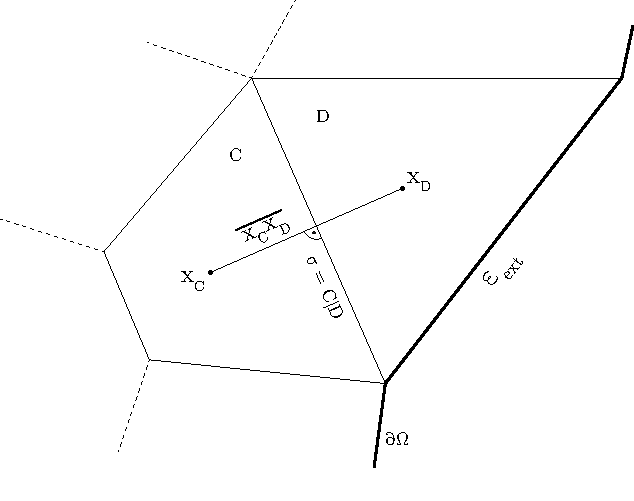
\includegraphics[width=0.5\linewidth]{diagrams/mesh.pdf}
        \caption{Visualisation of the cells $C, D$ in admissible mesh alongside their centroids $\vec{x}_C, \vec{x}_D$, their shared boundary $\sigma = C|D$ and their connecting line $\overline{\vec{x}_C\vec{x}_D}$. This visualisation was adapted from \cite{Strachota2018MatAnalisi}.} 
        \label{fig:mesh diagram}
    \end{figure}
    
    \section{Structured mesh} \label{sec: Structured mesh}
    We define a structured mesh that will be used in the majority of the text. Let $\Omega = (0, L_{0x}) \times (0, L_{0y}) \subset \R^2$ where $L_{0x}$ resp. $L_{0y}$ is the size of the domain along the $\vec{e}_1$ resp. $\vec{e}_2$. We divide this domain into $n_x$, $n_y \in \Nats$ equally sized rectangular cells $\mathcal{C}$ along the vectors $\vec{e}_1$ and $\vec{e}_2$ respectively and define $\dx := L_{0x}/n_x$, $\dy := L_{0y}/n_y$. This means that for each cell $C \in \Cells$, $m(C) = \dx\dy$ and for each face $\sigma \in \Faces$, $\hat{m}(\sigma) \in \{\dx, \dy\}$.

    
    \subsection{Finite volume discretization of Laplacian}
        We derive the approximation of Laplacian using the finite volume formalism. Because of the regular grid, this approximation can be equally obtained using the finite difference method. Let us consider a general function $\Psi:C^2(\Omega)\to\R$ and a cell $C \in \mathcal{C}$. Then
    
        \begin{align}
        \int_C\laplace{\Psi}(\vec{x})\,\dd x 
            &= \int_{\partial C}\nabla{\Psi}(\vec{x}) \cdot \vec{n}\,\dd S \label{laplacian dicretization 1} \\  
            &= \sum_{\sigma \in \varepsilon_C} \int_{\sigma} \nabla{\Psi}(\vec{x}) \cdot \vec{n} \,\dd S \label{laplacian dicretization 2} \\   
            &= \sum_{\sigma \in \varepsilon_C, \exists \vec{x}_\sigma \in \sigma} m(\sigma)\nabla{\Psi(\vec{x}_\sigma)} \cdot \vec{n_{\sigma}} \label{laplacian dicretization 3} 
        \end{align}
        where $\vec{n_{k,\sigma}}$ is the normal vector to $\sigma$.
        The divergence theorem was used in (\ref{laplacian dicretization 1}) and the mean value theorem to guarantee existence of such $\vec{x}_\sigma$ in (\ref{laplacian dicretization 3}). 
        
        \noindent
        Next we transition to the mesh function $\Psi_d$ and use
        \begin{align}
            \nabla \Psi(\vec{x}_\sigma) \cdot \vec{n}_\sigma \approx \frac{\Psi_D - \Psi_C}{\rho(\vec{x}_C, \vec{x}_D)} \label{eq: finite volume gradient substitution}
        \end{align}
        for cell $D$ adjacent to $C$ and $\sigma = C|D$. 
        Additionally for quantities $m(\sigma)$ and $\rho(\vec{x}_C, \vec{x}_D)$ holds
        \begin{align}
            m(\sigma) &= \begin{cases}
                \dy \text{ if $\sigma \parallel \vec{e}_1$ } \\
                \dx \text{ if $\sigma \parallel \vec{e}_2$ }
            \end{cases}, \\
            \rho(\vec{x}_C, \vec{x}_D) &= \begin{cases}
                \dx \text{ if $\sigma \parallel \vec{e}_1$ } \\
                \dy \text{ if $\sigma \parallel \vec{e}_2$ }
            \end{cases},
        \end{align}

        \noindent
        thus expanding (\ref{laplacian dicretization 3}) yields
        \begin{align}
        \int_C\laplace{\Psi}\,\dd x &\approx
            \sum_{\sigma \in \varepsilon_C\text{, }\sigma = C|D} m(\sigma)\frac{\Psi_D - \Psi_C}{\rho(\vec{x}_C, \vec{x}_D)} \\
            &=\frac{\dy}{\dx} (\Psi_E - \Psi_C) 
            - \frac{\dy}{\dx} (\Psi_W - \Psi_C) 
            + \frac{\dx}{\dy} (\Psi_N - \Psi_C) 
            - \frac{\dx}{\dy} (\Psi_S - \Psi_C)  \\
            &= \frac{\dy}{\dx} (\Psi_E - 2\Psi_C + \Psi_W) 
            + \frac{\dx}{\dy} (\Psi_N - 2\Psi_C + \Psi_S), \label{eq:finite volume first laplacian integral} \
        \end{align}
        where $E, W, N, S \in \Cells$ are cells adjacent to $C$ as shown on Figure \ref{fig:finite volume discretization}. This expression is only valid for $C \in \CellsInt$ as it requires all neighbouring cells to exist. We will however use this form on the entire $\Cells$ by defining additional "ghost cells" so that each cell in $\Cells$ has all neighbours. We discuss the formulation and values of ghost cells with regards to different boundary conditions in Section \ref{sec: boundary conditions}.
        \noindent
        
        \begin{figure}[!ht]
            \centering
            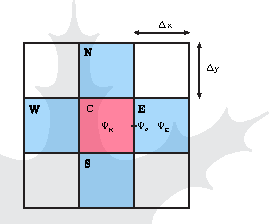
\includegraphics[height=5.4cm]{diagrams/finite_volume_discretization_2.pdf}
            \caption{
                Cells around the cell $C$ on regular grid $\Cells$. The cells are $\dx$, $\dy$ sized in the $\vec{e}_1$, $\vec{e}_2$ directions respectively. The mesh function $\Psi$ is defined at the center of each cell. $\Psi_\sigma$ is located on the shared boundary $\sigma$ between cells $C$ and $E$, written as $\sigma = C|E$. The value of $\Psi_\sigma$ is obtained by interpolation of the values of $\Psi$ in the adjacent cells $\Psi_C$ and $\Phi_E$. For this simple regular grid linear interpolation is used.
            }
            \label{fig:finite volume discretization}
        \end{figure}
        \FloatBarrier

        \noindent
        Note that by dividing the equation (\ref{eq:finite volume first laplacian integral}) by the volume of the cell $C$, we obtain
        \begin{align}
            \frac{1}{m(C)}\int_C\laplace{\Psi}\,\dd x 
                   \approx \frac{\Psi_E - 2\Psi_C + \Psi_W}{\dx^2} + \frac{\Psi_N - 2\Psi_C + \Psi_S }{\dy^2} =: \dlaplace \Psi_C \label{Psi laplacian appoximation},
        \end{align} 
        which is the second order central difference approximation of the Laplacian. We take this approximation as the definition of the discrete Laplacian $\dlaplace$ acting on mesh function $\Psi_d$.

    \subsection{Finite volume discretization of gradient}
        Repeating a similar procedure as for the approximation of Laplacian, we can write
        \begin{align}
            \int_{C}\nabla \Psi \,\dd x 
            &= \int_{\partial C} \Psi \cdot \vec{n}\,\dd s 
            = \sum_{\sigma \in \epsilon_C} \int_{\sigma} \Psi \cdot \vec{n}\,\dd s \\
            &= \sum_{\sigma \in \epsilon_C, \exists \vec{x}_\sigma \in \sigma} 
                m(\sigma)\Psi(\vec{x}_\sigma) \cdot \vec{n_\sigma} \\
            &\approx \sum_{\sigma \in \epsilon_C} 
                m(\sigma)\Psi_\sigma \cdot \vec{n_\sigma} \label{eq: approx laplace psi 3}
        \end{align}

        \noindent
        We employ second order approximation of $\Psi_\sigma$ for the cell face $\sigma = C|D$
        \begin{align}
            \Psi_\sigma = \frac{\rho(\vec{x}_C, \sigma)\Psi_D + \rho(\vec{x}_D, \sigma)\Psi_C}{\rho(\vec{x}_C, \vec{x}_D)} = \frac{1}{2}(\Psi_D + \Psi_C) \label{central diff grad},
        \end{align}
        where the mesh property $\rho(\vec{x}_C, \sigma) = \frac{1}{2}\rho(\vec{x}_C, \vec{x}_D)$ was used.

        \noindent
        Expanding (\ref{eq: approx laplace psi 3}) yields
        \begin{align}
            \int_{C}\nabla \Psi \,\dd x  
            &\approx \frac{\dy}{2} (\Psi_E + \Psi_C) \begin{pmatrix} 1  \\ 0 \end{pmatrix}
                + \frac{\dy}{2} (\Psi_W + \Psi_C) \begin{pmatrix} -1 \\ 0  \end{pmatrix} \\
                &+ \frac{\dx}{2} (\Psi_N + \Psi_C) \begin{pmatrix} 0  \\ 1  \end{pmatrix}
                + \frac{\dx}{2} (\Psi_S + \Psi_C) \begin{pmatrix} 0  \\ -1 \end{pmatrix} \\
            &= \frac{1}{2}\begin{pmatrix} 
                \dy (\Psi_E - \Psi_W) \\
                \dx (\Psi_N - \Psi_S)
            \end{pmatrix}
        \end{align}
        Similar to the discretization of Laplacian, this expression is only valid on $\CellsInt$ but by utilizing ghost cells we are able to extend it to the entire set of cells $\Cells$.  

        \vvskip
        Dividing by volume of cell $C$ gives
        \begin{align}
            \frac{1}{m(C)}\int_C\nabla{\Psi}\,\dd x
                   \approx \begin{pmatrix} 
                        \bigfrac{\Psi_E - \Psi_W}{2\dx} \\[8pt]
                        \bigfrac{\Psi_N - \Psi_S}{2\dy}
                   \end{pmatrix} \label{Psi gradient appoximation} =: \dnabla \Psi_C,
        \end{align}
        \noindent 
        which is the second order central difference approximation of gradient. We take this approximation as the definition of the discrete gradient $\dnabla$ acting on mesh function $\Psi_d$.

\subsection{Boundary conditions in the finite volume method} \label{sec: boundary conditions}
    We formulate Dirichlet, Neumann and periodic boundary conditions in a two dimensional finite volume discretization using the so called ghost cells \cite{LeVeque_2002FVMGhostCells}. Set of ghost cells $\Ghosts$ are added along the boundary of the domain $\Omega$ such that
    \begin{align}
        \forall \sigma \in \varepsilon_\text{ext} \exists C \in \Cells, G \in \Ghosts : \sigma = C|G.
    \end{align}
    We will use the same notation as in Section \ref{def: admissable mesh} for ghost cells $\Ghosts$ as for the cells $\Cells$. We will extend the domain of all mesh functions $\Psi_d$ to centroids of $\Cells \cup \Ghosts$.

    \subsubsection{Dirichlet boundary condition} \label{sec: Dirichlet boundary condtions}
    The Dirichlet boundary condition for function $\Psi:\Domain \to \R$ is written as
    \begin{align}
        \Psi|_{\partial \Domain} = f,
    \end{align}
    where $f:\partial \Domain \to \R$ prescribes values at the boundary. 

    We wish to express this for mesh function $\Psi_d$ on a single cell face $\sigma \in \FacesExt$. Let $C \in \Cells, G \in \Ghosts$ such that $\sigma = C|G$. We use the interpolation (\ref{central diff grad}) of mesh function $\Psi_d$ for value at the cell face $\Psi_\sigma$. The boundary condition becomes
    \begin{align}
        \Psi_\sigma = \frac{\rho(\vec{x}_C, \sigma)\Psi_G + \rho(\vec{x}_G, \sigma)\Psi_C}{\rho(\vec{x}_C, \vec{x}_G)} = f_\sigma \label{eq:Psi interp},
    \end{align}
    where $f_\sigma$ prescribes values at the cell face. From (\ref{eq:Psi interp}) we obtain 
    \begin{align}
        \Psi_G = \frac{f_\sigma \rho(\vec{x}_C, \vec{x}_G) - \rho(\vec{x}_G, \sigma) \Psi_C}{\rho(\vec{x}_C, \sigma)},
    \end{align}
    which for the regular grid as defined in Section \ref{sec: Structured mesh} becomes   
    \begin{align}
        \Psi_G = 2 f_\sigma - \Psi_c.
    \end{align}
    
    \subsubsection{Neumann boundary condition} \label{sec: Neumann boundary condtions}
    Reusing the same notation, the Neumann boundary condition states
    \begin{align}
        \nabla \Psi \cdot \vec{n}|_{\partial \Domain} = f,
    \end{align}
    where $\vec{n}$ is the outer normal vector of $\partial \Domain$ in the given point. Using the substitution for gradient operator (\ref{eq: finite volume gradient substitution}) and admissability of mesh $\Cells$, we can rewrite the boundary condition for mesh function $\Psi_d$ and prescribed value $f_\sigma$ as
    \begin{align}
        \frac{\Psi_G - \Psi_C}{\rho(\vec{x}_G, \vec{x}_C)} = f_\sigma,
    \end{align}
    thus the value at the ghost cell centroid is 
    \begin{align}
        \Psi_G = f_\sigma \rho(\vec{x}_G, \vec{x}_C) + \Psi_C.
    \end{align}
    For regular grid meshes, $\rho(\vec{x}_G, \vec{x}_C)$ is equal to $\dx$ resp. $\dy$, when $\sigma \parallel \vec{e}_2$ resp. $\sigma \parallel \vec{e}_1$.

    \subsubsection{Periodic boundary condition} \label{sec: Periodic boundary condtions}
    The periodic boundary condition is given only for regions $\Domain = (A_1, B_1)\times(A_2, B_2)\times \ldots\times(A_n, B_n)$, where $n \in \Nats$ and $ \vec{A}, \vec{B}\in \R^n$. Let $\vec{x}, \vec{y}\in \partial \Domain$ such that $x_i = A_i, y_i = B_i$ for some $i \in \hat{n}$, then the periodic boundary condition states
    \begin{align}
        \Psi(\vec{x}) = \Psi(\vec{y}).
    \end{align}
    That is, the values on the domain boundary $\partial \Domain$ are equal to the values on the opposite boundary.

    To formulate this for mesh function $\Psi_d$, no ghost cells are necessary. Instead, for the regular grid mesh, we define indexing $\forall i \in \hat{n}_y, j \in \hat{n}_x$ 
    \begin{align}
        \Psi_{i,j} := \Psi_d((j-1)\dx, (i-1)\dy) \label{def: 2D indexing}
    \end{align}
    and write the periodic boundary condition as
    \begin{align}
        \Psi_{1,j} = \Psi_{n_y, j}, \\
        \Psi_{i,1} = \Psi_{i, n_x}.
    \end{align}
    


\subsection{Finite volume discretization of the phase field equations} \label{sec:semidiscrete scheme}
    We use the already derived formulas to discretize the Phase field model. Let $\Phi_d:\Timeint \times\Centroids \to \R$ resp. $T_d:\Timeint \times\Centroids \to \R$ be the mesh function substitution of phase resp. heat field. By integrating both sides of equations (\ref{Allen-Cahn kform T}), (\ref{Allen-Cahn kform Phi}) over a cell $C$, using formulas (\ref{Psi laplacian appoximation}), (\ref{Psi gradient appoximation}) and substituting 
    \begin{align}
        &\frac{1}{m(C)}\int_C\dert{\Phi} \dd x \approx \ddt{\Phi_C} \\
        &\frac{1}{m(C)}\int_C k_1(\nabla \Phi) \dd x \approx k_1(\dnabla\Phi_C) \\
        &\frac{1}{m(C)}\int_C k_2(\Phi, \nabla \Phi) \dd x \approx k_2(\Phi_C, \dnabla\Phi_C), \\
        &\frac{1}{m(C)}\int_C k_3(\nabla \Phi) \dd x \approx k_3(\dnabla\Phi_C) 
    \end{align}
    we obtain the semi-discrete scheme of the Phase field model $\forall C \in \Cells$
    \begin{align}
        \ddt{T_C}
            &= \dlaplace T_C + L\ddt{\Phi_C} &&\text{ in } \Timeint, \label {eq: Semidiscrete Phi} \\
        \ddt{\Phi_C}
            &= k_1(\dnabla\Phi_C)\dlaplace{\Phi}_C + k_0(\Phi_C, \dnabla\Phi_C) + k_2(\dnabla\Phi_C)(T^* - T_C) &&\text{ in } \Timeint, \label{eq: Semidiscrete T} \\
        T_C|_{t=0} &= T_{C,\text{ini}}|_{\Centroids}, \\ 
        \Phi_C|_{t=0} &= \Phi_{C,\text{ini}}|_{\Centroids},
    \end{align}
    alongside Dirichlet, Neumann, or periodic boundary conditions for both $T_d$ and $\Phi_d$ as specified in Sections \ref{sec: Dirichlet boundary condtions}, \ref{sec: Neumann boundary condtions} and \ref{sec: Periodic boundary condtions}.

\chapter{Time integration schemes}  \label{chap:time integration schemes}
\section{Explicit integration schemes} \label{sec: explicit scheme}
    The semi-discrete scheme in Section \ref{sec:semidiscrete scheme} forms an initial value problem, for which a solution can be obtained using explicit time integration schemes. We evaluated and compared explicit Euler method, fourth order Runge-Kutta method and fourth order Runge-Kutta-Merson method. We will refer to the resulting schemes utilizing these methods as Euler, RK4 and RKM in order.
    
    In Algorithm \ref{alg:Euler time integration} we illustrate time integration procedure going from time step $n$ to $n+1$ using the explicit Euler method defined as 
    \begin{align}
        \frac{\dd \Psi^n}{\dd t} \approx \frac{\Psi^{n+1} - \Psi^n}{\dt},
    \end{align}
    where $\Psi^{n} := \Psi(n\dt)$, $\Psi \in \{\Phi_C, T_C\}$, $C \in \Cells$ using time step $\dt > 0$ and time step index $n \in \Nats$.
    
    \begin{algorithm}[!ht]
    \caption{Time integration using the explicit Euler method}\label{alg:Euler time integration}
        \begin{algorithmic}
            \setstretch{2}
            \For{each cell $C \in \Cells$}
                \State $\dlaplace T_C^n \gets \bigfrac{T_E^n - 2T_C^n + T_W^n}{\dx^2} + \bigfrac{T_N^n - 2T_C^n + T_S^n}{\dy^2}$
                \State $\dlaplace \Phi_C^n \gets \bigfrac{\Phi_E^n - 2\Phi_C^n + \Phi_W^n}{\dx^2} + \bigfrac{\Phi_N^n - 2\Phi_C^n + \Phi_S^n}{\dy^2}$
                \State $\dnabla \Phi_C^n \gets 
                    \begin{pmatrix} 
                        \bigfrac{\Phi_E^n - \Phi_W^n}{2\dx}  \\[6pt]
                        \bigfrac{\Phi_N^n - \Phi_S^n}{2\dy}
                   \end{pmatrix}$
                   
                \State $\ddt{T_C^n} \gets k_1(\dnabla\Phi_C^n)\dlaplace\Phi_C^n + k_0(\Phi_C^n, \dnabla\Phi_C^n) + k_2(\dnabla\Phi_C^n)(T^* - T_C^n)$
                \State $\ddt{T_C^n} = \dlaplace T_C^n + L\ddt{\Phi_C^n}$
                \State $\Phi_C^{n+1} \gets \Phi_C^n + \dt\ddt{T_C^n}$
                \State $T_C^{n+1} \gets T_C^n + \dt\ddt{T_C^n}$
            \EndFor
        \end{algorithmic}
    \end{algorithm}
    \FloatBarrier

    \subsection{Runge-Kutta-Merson method}
    For completeness we include algorithm of the fourth order Runge-Kutta-Merson method \cite{ChristiansenRKM1970} and \cite{StrachotaDizertation}. This method is used to solve system of differential equations in the form 
    \begin{align}
        \dert{\vec{x}} = \vec{f}(t, \vec{x}),
    \end{align}
    where $\vec{x} \in \R^N$ is the unknown vector function and $\vec{f}:\Timeint \times \R^N \to \R^N$ is the function of right hand side with $N \in \Nats$. The Runge-Kutta-Merson algorithm is shown in Algorithm \ref{alg:Runge-Kutta-Merson method} below. 

    \begin{algorithm}[!ht]
        \caption{Runge-Kutta-Merson method}\label{alg:Runge-Kutta-Merson method}
        \begin{algorithmic}
            \State Let $\vec{f}:\R^{1 +N} \to \R^N$ be the numerically integrated function with $N \in \Nats$. 
            \State Let $\dt_{ini} \in \R$ resp. $\vec{x}_{ini} \in \R^N$ be the initial timestep resp. initial condition.
            \State Let $t \in \R$ be the current time level, $T \in \R$ final time and $\varepsilon \in \R$ target integration error.
            \State $\dt = \dt_{ini}$
            \State $\vec{x} = \vec{x}_{ini}$
            \Loop
                \If{$T - t < \dt$}
                    \State $\dt = T - t$
                \EndIf
                
                \State $\vec{K}_1 = \vec{f}(t, \vec{x})$
                \State $\vec{K}_2 = \vec{f}(t + \frac{\dt}{3}, \vec{x} + \frac{\dt}{3}\vec{K}_1)$
                \State $\vec{K}_3 = \vec{f}(t + \frac{\dt}{3}, \vec{x} + \frac{\dt}{6}(\vec{K}_1 + \vec{K}_2))$
                \State $\vec{K}_4 = \vec{f}(t + \frac{\dt}{2}, \vec{x} + \frac{\dt}{8}(\vec{K}_1 + 3\vec{K}_2))$
                \State $\vec{K}_5 = \vec{f}(t + \dt, \vec{x} + \frac{\dt}{2}(\vec{K}_1 - 3\vec{K}_3 + 4\vec{K}_4))$
                \State $\delta = \frac{\dt}{3}\norm{0.2\vec{K}_1 - 0.9\vec{K}_3 + 0.8\vec{K}_4 - 0.1\vec{K}_5}_{\infty}$
    
                \If{$\delta < \varepsilon$}
                    \State $\vec{x} \gets \vec{x} + \frac{\dt}{6}(\vec{K}_1 + 4\vec{K}_4 + \vec{K}_5)$
                    \State $t \gets t + \dt$
                    \If{$t \ge T$}
                        \State \textbf{break}
                    \EndIf
                \EndIf
                
                \If{$\delta > 0$}
                    \State $\dt \gets \left( \frac{\varepsilon}{\delta} \right)^{0.2} \cdot \dt$
                \EndIf
            \EndLoop
        \end{algorithmic}
    \end{algorithm}
    \FloatBarrier  


\newpage
\section{Semi-implicit integration scheme} \label{sec: semi implicit scheme}
    We derive semi-implicit time integration scheme of the semi-discrete scheme (S-I) given in Section \ref{sec:semidiscrete scheme} using the Crank-Nicolson method \cite{CrankNicolson1947}. One advatnage of the Crank-Nicolson method over the previously described explicit methods is its unconditional stability \cite{Thomas1998Numerical}.
    \subsection{Coupled integration scheme}
    For simplicity of notation, let us denote $\Phi := \Phi_C$, $\nabla \Phi := \nabla_d \Phi_C$, $\laplace{\Phi} := \laplace_d \Phi_C$ for some cell $C$. Similarly $T := T_C$, $\laplace{T} := \laplace_d T_C$. 
    
    % We attempt to formulate the Allen-Cahn equations into the form of a matrix equation $\mat{A}\vec{x} = \vec{b}$ for some matrix $\mat{A}$, vector of right hand side $\vec{b}$ and vector $\vec{x}$ of unknown variables $\Phi, T$ at the next time step. By calculating $A$, $b$ using the information at the current time step $n$ we can solve for $\vec{x}$ to obtain the next state at time step $n + 1$. 
    
    First we time discretize the equations (\ref{Allen-Cahn kform T}), (\ref{Allen-Cahn kform Phi}) by applying more general form of the Crank-Nicolson time discretization given by 
    \begin{align}
        \frac{\Psi^{n+1} - \Psi^n}{\dt} \approx \gamma\dert{\Psi^{n+1}} + (1 - \gamma)\dert{\Psi^n} \label{eq: Crank-Nicolson}
    \end{align}
    % for some general function $\Psi:\R\to\R$ and
    for $\gamma \in [0, 1]$. By setting $\gamma = 0$ we obtain explicit Euler method, by setting $\gamma = 1/2$ we obtain the Crank-Nicolson method \cite{CrankNicolson1947} and by setting $\gamma = 1$ the implicit Euler method. Applying this discretization to the semi-discrete scheme in Section \ref{sec:semidiscrete scheme} yields
    \begin{align}
        \frac{T^{n+1} - T^n}{\dt} 
            &\approx \gamma\left[\laplace{T^{n+1}} + L\dert{\Phi^{n+1}} \right] 
             + (1 - \gamma)\left[\laplace{T^{n}} + L\dert{\Phi^{n}} \right]  \label{Crank Nicolson T}, \\
        \frac{\Phi^{n+1} - \Phi^n}{\dt} 
            &\approx \gamma \left[ k_1(\nabla\Phi^{n+1})\laplace{\Phi^{n+1}} + k_0(\Phi^{n+1}, \nabla\Phi^{n+1}) + k_2(\nabla\Phi^{n+1})(T^* - T^{n+1}) \right]  \notag \\
            &+ (1 - \gamma)\left[k_1(\nabla\Phi^{n})\laplace{\Phi^{n}} + k_0(\Phi^{n}, \nabla\Phi^{n}) + k_2(\nabla\Phi^{n})(T^* - T^{n})\right]. \label{Crank Nicolson Phi 0}         
    \end{align}
    
    Since $k_0, k_1, k_2$ are nonlinear, we cannot evaluate them at point $\Phi^{n+1}$, thus an approximation $k_i(\Phi^{n+1}) \approx k_i(\Phi^n)$ is used for $i \in \{1, 2, 3\}$. Because now all $k_i$ functions are evaluated in the same timestep, we drop the argument notation and denote $k_0 := k_0(\Phi^{n}, \nabla\Phi^{n})$, $k_1 := k_1(\nabla\Phi^{n})$, $k_2 := k_2(\nabla\Phi^{n})$. Thus (\ref{Crank Nicolson Phi 0}) becomes
    \begin{align}
        \frac{\Phi^{n+1} - \Phi^n}{\dt} 
            &= \gamma\left[ k_1\laplace{\Phi^{n+1}} + k_0 + k_2(T^* - T^{n+1}) \right] \nonumber \\
            &+ (1 - \gamma)\left[ k_1\laplace{\Phi^{n}} + k_0 + k_2(T^* - T^{n}) \right]. \label{Crank Nicolson Phi}
    \end{align}

    \noindent
    By multiplying (\ref{Crank Nicolson Phi}) by $\dx$ and isolating all terms containing $T^{n+1}$, $\Phi^{n+1}$ in (\ref{Crank Nicolson Phi}), (\ref{Crank Nicolson T}) we obtain
    \begin{align}
        T^{n+1} - \dt\gamma(\laplace{T^{n+1}} + L\dert{\Phi^{n+1}})
            &= T^n + \dt(1 - \gamma)(\laplace{T^{n}} + L\dert{\Phi^{n}}) \label{eq: Heat implicit almost done}, \\
        \Phi^{n+1} - \dt\gamma(k_1\laplace{\Phi^{n+1}} - k_2 T^{n+1})
            &= \Phi^n + \dt(1 - \gamma)(k_1\laplace{\Phi^{n}} - k_2 T^{n}) + \dt(k_0 + k_2 T^*) \label{Phi coupled EQ}.
    \end{align}

    \noindent
    Substituting $\dert{\Phi^{n+1}} \approx \frac{\Phi^{n+1} - \Phi^n}{\gamma\dt} - \frac{1 - \gamma}{\gamma}\dert{\Phi^n}$ in equation (\ref{eq: Heat implicit almost done}) derived from (\ref{eq: Crank-Nicolson}), and shuffling terms yields
    \begin{align}
        T^{n+1} - \dt\gamma\laplace{T^{n+1}} - L\Phi^{n+1}
            &= T^n - L\Phi^n + \dt(1 - \gamma)\laplace{T^{n}}. \label{T coupled EQ}
    \end{align}
    
    \noindent
    Now we transition from a notation in terms of general cell $C$ to using its indices $(i, j) \in \hat{n}_y\times\hat{n}_x$. 
    Let $\vec{P} \in \R^N$ with $N := n_x n_y$ be vector representation of the mesh function $\Psi:\Cells \to \R$ such that $\forall j \in \hat{n}_x, i \in \hat{n}_y$: $\vec{P}_{j + n_x(i - 1)} = \Psi((j-1)\dx, (i-1)\dx) = \Psi_{i,j} = \Psi_C$. 
    Using the discrete Laplacian $\dlaplace \Psi$ (\ref{Psi laplacian appoximation}), discrete gradient $\dnabla \Psi$ (\ref{Psi gradient appoximation}) and describing cells $E$, $W$, $N$, $S$ using indices with respect to cell at $(i, j) \in \hat{n}_y\times\hat{n}_x$ we define its vector equivalent
    \begin{align}
        \dlaplace \vec{P}_{j+n_x(i - 1)}
            &:= \frac{\vec{P}_{j+1+n_x(i - 1)} - 2\vec{P}_{j+n_x(i - 1)} + \vec{P}_{j-1+n_x(i - 1)}}{\dx^2} \nonumber \\
            &+ \frac{\vec{P}_{j+n_xi} - 2\vec{P}_{j+n_x(i - 1)} + \vec{P}_{j+n_x(i - 2)}}{\dy^2} \label{Coupled laplace approx}, \\
        \dnabla \vec{P}_{j+n_x(i - 1)} &:= \begin{pmatrix} 
            \bigfrac{P_{j+1 + n_x(i - 1)} - P_{j-1 + n_x(i - 1)}}{2\dx} \\[8pt]
            \bigfrac{P_{j + n_xi} - P_{j + n_x(i - 2)}}{2\dy}
       \end{pmatrix}. \label{Coupled grad approx}
    \end{align}
    We define $\vec{F}, \vec{U} \in \R^N$ such that $\forall j \in \hat{n}_x, i \in \hat{n}_y$
    \begin{align}
        \vec{F}_{j + n_x(i - 1)} &= \Phi_{i,j}, \label{def: vector state notation} \\
        \vec{U}_{j + n_x(i - 1)} &= T_{i,j}, \label{def: vector state notation U}
    \end{align}
    where $\Phi_{i,j}, T_{i,j}$ are given by (\ref{def: 2D indexing}).
    
    Rewriting equations (\ref{U coupled EQ}) and (\ref{Phi coupled EQ}) in terms of $\vec{U}$ and $\vec{F}$ using the equations (\ref{Coupled laplace approx}), for $\dlaplace$ and (\ref{Coupled grad approx}) for $\dnabla$ yields
    \begin{align}
        \vec{U}^{n+1} - \dt\gamma\dlaplace{\vec{U}^{n+1}} - L\vec{F}^{n+1}
            &= \vec{U}^n - L\vec{F}^n + \dt(1 - \gamma)\dlaplace{\vec{U}^{n}} \label{U coupled EQ}, \\
        \vec{F}^{n+1} - \dt\gamma(k_1\dlaplace{\vec{F}^{n+1}} - k_2 T^{n+1})
            &= \vec{F}^n + \dt(1 - \gamma)(k_1\dlaplace{\vec{F}^{n}} - k_2 T^{n}) + \dt(k_0 + k_2 T^*) \label{F coupled EQ},
    \end{align}
    which can be expressed as a system of linear equations in the form 
    \begin{align}
        \begin{pNiceArray}{c c}
            A_F & B_F \\
            B_U & A_U
        \end{pNiceArray} 
        \begin{pNiceArray}{c}
            \vec{F} \\ 
            \vec{U}
        \end{pNiceArray} 
        = 
        \begin{pNiceArray}{c}
            \vec{b}_F \\ 
            \vec{b}_U
        \end{pNiceArray} 
    \end{align}
    with the values of $A_F$, $B_F$, $B_U$, $A_U$ $\in \R^{N\times N}$ and vectors of right hand side $\vec{b}_F$, $\vec{b}_U$ $\in \R^N$ given by $\forall (k,l)\in \hat{N}\times\hat{N}$ by
    \begin{align} 
        (A_F)_{k,l} &= \begin{cases} \label{eq:Semi-Implicit matrices}
            1 + k_1(\frac{2\gamma\dt}{\dx^2} + \frac{2\gamma\dt}{\dy^2}) & \text{ when $l = k$}, \\
            -k_1\frac{\gamma\dt}{\dx^2} & \text{ when $l+1 = k$}, \\
            -k_1\frac{\gamma\dt}{\dx^2} & \text{ when $l-1 = k$}, \\
            -k_1\frac{\gamma\dt}{\dy^2} & \text{ when $l+n_x = k$}, \\
            -k_1\frac{\gamma\dt}{\dy^2} & \text{ when $l-n_x = k$}, \\
            0                           & \text{ otherwise} \\
        \end{cases} \\
        \
        (B_F)_{k,l} &= \begin{cases}
            -\gamma\dt k_2 & \text{ when $l = k$}, \\
            0              & \text{ otherwise} \\
        \end{cases} \\
        \
        (A_U)_{k,l} &= \begin{cases}
            1 + \frac{2\gamma\dt}{\dx^2} + \frac{2\gamma\dt}{\dy^2} & \text{ when $l = k$}, \\
            -\frac{\gamma\dt}{\dx^2} & \text{ when $l+1 = k$}, \\
            -\frac{\gamma\dt}{\dx^2} & \text{ when $l-1 = k$}, \\
            -\frac{\gamma\dt}{\dy^2} & \text{ when $l+n_x = k$}, \\
            -\frac{\gamma\dt}{\dy^2} & \text{ when $l-n_x = k$}, \\
            0                        & \text{ otherwise} \\
        \end{cases}  \\
        \
        (B_U)_{k,l} &= \begin{cases}
            -L         & \text{ when $l = k$}, \\
            0          & \text{ otherwise} \\
        \end{cases} \\
        \
        (\vec{b}_F)_{k} &= \vec{F}_k^n + \dt(1 - \gamma)(k_1\dlaplace{\vec{F}_k^{n}} - k_2 \vec{U}_k^{n}) + \dt(k_0 + k_2 T^*), \\
        (\vec{b}_U)_{k} &= \vec{U}_k^n - L\vec{F}_k^n + \dt(1 - \gamma)\dlaplace{\vec{U}_k^{n}}.
    \end{align}
    In (\ref{eq:Semi-Implicit matrices}), the argument $\dlaplace \vec{F}_k^n$ for the $k_1, k_2, k_3$ functions was for readability of the expressions elided.
    
    Such system of linear equations can be solved by an appropriate matrix solver such as the Successive over-relaxation method (SOR) \cite{YoungDavid1950SOR}. However, in practice, with physically accurate choice of simulation parameters, this system is ill fit for numerical solvers. Observe that in the off diagonal matrix $B_U$ the only non-zero values are $-L$ without dependence on the mesh resolution $\dx$ or time step $\dt$. In our experiments we choose $L = 2$ making the matrix not diagonally dominant and causing the employed solver to diverge, regardless of choice for other model parameters.

    \subsection{Split integration scheme}
    The poor convergence of the coupled matrix scheme motivates us to attempt at least an approximate solution. One approach is to use the operator splitting method \cite{MacNamara2016OperatorSplitting}. The main idea is to split the complex problem into simpler sub-problems, solve each individually, then combine their solutions to obtain the final solution. In our case by solving the system of equations for the phase field and temperature field separately.

    We begin with the equations (\ref{U coupled EQ}) and (\ref{F coupled EQ}) and approximate the $\vec{U}^{n+1}$ term with $\vec{U}^n$ in the $\vec{F}$ equation then move it to the right side. Thus a new equation is obtained for the right hand side
    \begin{align}
        (\vec{b}_F)_{k} &= \vec{F}_k^n  +\dt(1 - \gamma)k_1\dlaplace{\vec{F}_k^{n}}  + \dt(k_0 + k_2(T^* - \vec{U}_k^{n})) && \forall k \in \hat{N}. \label{eq:semi implicit b_F}
    \end{align}

    This modification enables
    \begin{align}
        A_F^n \vec{F}^{n+1} = \vec{b}_F^{n} \label{eq:semi implicit A_F equation}
    \end{align}
    to be solved independently using only the current state $\vec{F}^n$ and yielding the new state $\vec{F}^{n+1}$. Since $\vec{F}^{n+1}$ is now known, we can move it to the right hand side of the equation (\ref{U coupled EQ}) giving us modified equation for its right hand side
    \begin{align}
        (b_U)_{k}^{n, n+1} &= \vec{U}_k^n - L(\vec{F}_k^{n+1} - \vec{F}_k^n) + \dt(1 - \gamma)\dlaplace{\vec{U}_k^{n}} && \forall k \in \hat{N}. 
    \end{align}
    which allows the new temperature field $\vec{U}^{n+1}$ to be solved for in the matrix equation
    \begin{align}
        A_U^n \vec{U}^{n+1} = \vec{U_F}^{n, n+1}. \label{eq:semi implicit A_U equation}
    \end{align}

    Notice that both $A_F^n$, $A_U^n$ are positively definite, symmetric matrices and with an appropriate choice of $\dx, \dy, \dt$ also diagonally dominant. This guarantees convergence for many matrix solvers and specifically allows the Conjugate gradient method to be used, which is given in Algorithm \ref{alg:Conjugate Gradient method}.
\subsubsection{Conjugate gradient method}
    For completeness, we include the Conjugate gradient method algorithm \cite{painless_conjugate_grad}. Conjugate gradient method is used to solve matrix equations in the form
    \begin{align}
        \mat{A}\vec{x} = \vec{b},
    \end{align}
    where $\vec{x} \in \R^N$ is the vector of unknowns, $\mat{A} \in \R^{N\times N}$ is symmetric, positive-semidefinite and $\vec{b} \in \R^N$. It is well suited for large sparse matrices such as those arising from the finite difference and finite element methods \cite{painless_conjugate_grad}. Since all operations are performed using vectors, it is amenable to parallel implementation. 
    
    \begin{algorithm}[!ht]
        \caption{Conjugate Gradient method}\label{alg:Conjugate Gradient method}
        \begin{algorithmic}
            \State Let $\mat{A} \in \R^{N\times N}$, $\vec{b} \in \R^N$ represent a system of linear equations with $N \in \Nats$. 
            \State Let $\vec{x}^0$ be initial guess at the solution and $\varepsilon \in \R$ tolerence for the residual
            \State Let $M \in \Nats$ be the maximum number of iterations.
            \State The output is $\vec{x} \in \R^N$ such that $\norm{\mat{A}\vec{x} - \vec{b}}_{\infty} < \varepsilon$.
            \State $\vec{d}^0 = \vec{r}^0 = \vec{b} - \mat{A}\vec{x}^0$
            \For{$k = 0, \dots, M$}
                \If{$\norm{\vec{r}^k}_{\infty} < \varepsilon$ or $k > M$}
                    \State $\vec{x} = \vec{x}^k$
                    \State \textbf{break}
                \EndIf
                
                \State $\alpha^k = \bigfrac{\vec{r}^k \cdot \vec{r}^k}{(\vec{d}^k)^T \mat{A} \vec{d}^k}$
                \State $\vec{x}^{k+1} = \vec{x}^{k} + \alpha^{k}\vec{d}^{k}$
                \State $\vec{r}^{k+1} = \vec{r}^{k} + \alpha^{k}\mat{A} \vec{d}^{k}$
                \State $\beta^k = \bigfrac{\vec{r}^{k+1} \cdot \vec{r}^{k+1}}{\vec{r}^k \cdot \vec{r}^k}$
                \State $\vec{d}^{k+1} = \vec{r}^{k+1} + \beta^{k+1}\mat{A} \vec{d}^{k}$
            \EndFor
        \end{algorithmic}
    \end{algorithm}
\FloatBarrier    

    
\section{Operator splitting corrections}
    We can rewrite the explicit and semi-implicit schemes in the form 
    \begin{align}
        \vec{F}^{n+1} &= S_F(\vec{F}^n, \vec{U}^n), \label{def: Timestepping functions} \\
        \vec{U}^{n+1} &= S_U(\vec{F}^{n+1}, \vec{U}^n), 
    \end{align}
    where $\vec{F}^n, \vec{U}^n \in \R^N$ are vectors of the phase resp. temperature field mesh functions $\Phi, T$, given by (\ref{def: vector state notation}) and (\ref{def: vector state notation U}) at timestep $n \in \Nats$. 
    $S_F, S_U:\R^N \times \R^N \to \R^N$ are functions encompassing the explicit and semi-implicit time integration schemes (see Sections \ref{sec: semi implicit scheme} and \ref{sec: explicit scheme}) used to calculate the next iteration of $\vec{F}^n, \vec{U}^n$ respectively. 
    
    For the explicit schemes the definition of $S_F, S_U$ can be given explicitly using the vectors $\vec{F}^n, \vec{U}^n$.
    For the semi-implicit scheme, $S_F, S_U$ are defined in terms of solution to the matrix equations (\ref{eq:semi implicit A_F equation}), (\ref{eq:semi implicit A_U equation}).
    
    Notice that the calculation of $\vec{F}^{n+1}$ uses $\vec{U}^n$, while the calculation $\vec{U}^{n+1}$ uses $\vec{F}^{n+1}$. Compared to equations in the semi-discrete scheme given in Section \ref{sec:semidiscrete scheme}
    \begin{align*}
        \ddt{T_C}
            &= \dlaplace T_C + L\ddt{\Phi_C}, \\
        \ddt{\Phi_C}
            &= k_1(\dnabla\Phi_C)\dlaplace{\Phi}_C + k_0(\Phi_C, \dnabla\Phi_C) + k_2(\dnabla\Phi_C)(T^* - T_C),
    \end{align*}
    where $\Phi$ depends on $T$ and vice versa at any point in time $t \in \Timeint$. In other words, there is bi-directional dependency between the two equations, but the current time integration schemes only models one direction.
    
    To quantify the error commited by the operator splitting techniques we define $n$-th \emph{step residual} $r_\Phi^n \in \R^N$ for both categories of time integration schemes as 
    
    \newcommand{\stepF}[0]{\vec{\mathcal{F}}}
    \newcommand{\stepU}[0]{\vec{\mathcal{U}}}
    \begin{align}
        r_\Phi^n 
            &:= S_F(\vec{F}^n, \vec{U}^n) - S_F(\vec{F}^n, \vec{U}^{n + 1}) \label{def: step residual},
    \end{align}
    which can be read as "the difference between vector $\vec{F}^n$ obtained using the information from the current time step and the vector$\stepF$ we would have obtained the temperature field vector $\vec{U}^{n+1}$ from the next time step was used".
    Note that $r_\Phi^n$ quantifies only the internal consistency of the approximations and makes no statement about the quality of the chosen approximations in relation to the exact solution of the original equations.

    \noindent
    Using the scheme functions (\ref{def: Timestepping functions}) we can rewrite (\ref{def: step residual}) as
    \begin{align*}
        r_\Phi^n 
            &= \vec{F}^{n+1} - S_F(\vec{F}^n, \vec{U}^{n+1}) \\
            &= \vec{F}^{n+1} - S_F(\vec{F}^n, S_U(\vec{F}^{n+1}, \vec{U}^n))
    \end{align*}
    and generalize its definition for a candidate vector $\stepF \in \R^N$ for the next step $\vec{F}^{n+1}$ as
    \begin{align}
        r_\Phi &= \stepF - S_F(\vec{F}^n, S_U(\stepF, \vec{U}^n)). \label{step residual}
    \end{align}
    
    \subsection{Repeated time stepping} \label{sec:repeated time stepping}
    We can lower the magnitude of the step residual $r_\Phi$, thus potentially increasing the accuracy of our model, by iterating the candidate $\stepF$ for the next step $\vec{F}^{n+1}$ repeatedly until the norm of step residual $r_\Phi^n$ falls below desired accuracy. The Algorithm \ref{alg:fractional timestepping} shows the procedure going from time step $n$ to $n+1$, while keeping $\norm{r_\Phi^n}$ small.
    
    \begin{algorithm}[!ht]
        \caption{Repeated time stepping correction}\label{alg:fractional timestepping}
        \begin{algorithmic}
            \State $\stepF^{0} \gets \vec{F}^n$
            \State $\stepU^{0} \gets \vec{U}^n$
            \For{$k = 1, \dots, M$}
                
                \State $\stepF \gets S_F(\vec{F}^n, \stepU^{k-1})$
                \State $\stepU \gets S_U(\vec{\stepF}, \vec{U}^n)$
                
                \State $r_\Phi \gets \stepF^{k-1} - \stepF$
                \If{$\norm{r_\Phi} < \varepsilon$}
                    \State $\stepF^{k} \gets \stepF$
                    \State $\stepU^{k} \gets \stepU$
                    \State \textbf{break}
                \EndIf
    
                \State $\stepF^{k} \gets (1-\alpha)\stepF^{k-1} + \alpha\stepF$
                \State $\stepU^{k} \gets (1-\alpha)\stepU^{k-1} + \alpha\stepU$
            \EndFor
            \State $\vec{F}^{n+1} \gets \stepF^{k}$ 
            \State $\vec{U}^{n+1} \gets \stepU^{k}$ 
        \end{algorithmic}
    \end{algorithm}
    In Algorithm \ref{alg:fractional timestepping}, $\varepsilon \in \R$ is the target step residual norm, $M \in \Nats$ is maximum number of iterations and $\alpha \in (0, 1]$ is a relaxation parameter to ensure convergence. Notice that for $\alpha = 1$ the formula $r_\Phi = \stepF^{k-1} - \stepF$ in the algorithm, matches the definition (\ref{step residual}) with $\stepF^{k-1}$ as the current candidate. This is because $\stepF = S_F(\vec{F}^n, S_U(\stepF^{k-1}, \vec{U}^n))$.

    From our testing with $\alpha = 1$ the Algorithm \ref{alg:fractional timestepping} drives down the step residual arbitrarily $r_\Phi^n$ low. However, for each iteration we have to perform the entire solution procedure anew. This means that when using the Algorithm \ref{alg:fractional timestepping} and performing $M$ iterations, the total runtime will be $M$ times longer then if the algorithm was not used.  

    \subsection{Correction term} \label{sec:correction term}   
    We can achieve similar results to $r_\Phi$ for almost no additional cost by making the the $\Phi$ equation "more implicit". We start by considering the explicit Euler time discretization of the heat equation (\ref{Allen-Cahn kform T})
    \begin{align}
        \frac{T^{n+1} - T^n}{\dt} 
            &\approx \laplace{T^{n}} + L\dert{\Phi^{n}}\\
    \end{align}
    and factor out $T^{n+1}$ 
    \begin{align}
        T^{n+1} &= T^n + \dt\laplace{T^{n}} + \dt L\dert{\Phi^{n}}.\\
    \end{align}
    Substituting $T^{n+1}$ for $T$ in the phase field equation (\ref{Allen-Cahn kform Phi}) we obtain 
    \begin{align}
        \dert{\Phi} 
            &= k_1(\nabla\Phi)\laplace{\Phi} + k_0(\Phi, \nabla\Phi) + k_2(\nabla\Phi)(T^* - T - \dt\laplace{T - \dt L\dert{\Phi}}) 
    \end{align}
    We dropped the $T^n$ notation in favor of $T$ since we consider the resulting equation a brand new object instead of time discretized version of the equation (\ref{Allen-Cahn kform Phi}). 
    
    \noindent
    Rearranging so that we isolate $\dert{\Phi}$ yields
    \begin{align}
        \dert{\Phi}
            &= \frac{k_1(\nabla\Phi)\laplace{\Phi} + k_0(\Phi, \nabla\Phi) + k_2(\nabla\Phi)(T^* - T - \dt\laplace{T})}{1 + \dt Lk_2(\nabla\Phi)} \label{Corrected Regular grid Phi}
    \end{align}

    \newcommand{\tk}[0]{\Tilde{k}}
    \newcommand{\td}[0]{\Tilde{d}}

    \noindent
    By defining rescaled nonlinear functions
    \begin{align}
        \tk_0(\Phi, \nabla\Phi) := \frac{k_0(\Phi, \nabla\Phi)}{1 + \dt Lk_2(\nabla\Phi)},
        &&\tk_1(\nabla\Phi) := \frac{k_1(\nabla\Phi)}{1 + \dt Lk_2(\nabla\Phi)},
        &&\tk_2(\nabla\Phi) := \frac{k_2(\nabla\Phi)}{1 + \dt Lk_2(\nabla\Phi)},
    \end{align}
    we can rewrite the modified equation into a form very closely matching the original (\ref{Allen-Cahn kform Phi})
    \begin{align}
        \dert{\Phi}
            &= \tk_1(\nabla\Phi)\laplace{\Phi} + \tk_0(\Phi, \nabla\Phi) + \tk_2(\nabla\Phi)(T^* - T - \dt\laplace{T})
    \end{align}

    % We can transition to the semi-discrete formulation and as in the semi-implicit time integration scheme section use $\Phi := \Phi_C$, $\nabla \Phi := \nabla_d \Phi_C$, $\laplace{\Phi} := \laplace_d \Phi_C$, $T := T_C$, $\laplace{T} := \laplace_d T_C$ for some cell $C$. 
    Upon transition to mesh functions and discrete operators this combined with the temperature filed equation (\ref{eq: Semidiscrete T}) forms a different "corrected" semi-discrete scheme. Note that the constant $\dt$ in this semi-discrete scheme only makes sense in context of time integration schemes that are performed without intermediate time steps, that is the explicit Euler scheme and semi-implicit scheme. Still, all previously discussed time integration schemes can be rederived for this corrected scheme and behave consistently. 
    
    For the explicit schemes the change can be derived trivially by. Its worth noting that all of the additional terms in (\ref{Corrected Regular grid Phi}) were already being calculated in each time step, thus this "corrected" version has negligible added simulation runtime cost.

    To derive the "corrected" semi-implicit time integration scheme we perform the same steps as when deriving the semi-discrete scheme in Section \ref{sec: semi implicit scheme}. The resulting matrices $A_F^n, A_U^n$ are the same as (\ref{eq:Semi-Implicit matrices}) but $k_1$, $k_2$ and $k_3$ are replaced with their rescaled counterparts $\tk_1$, $\tk_2$ and $\tk_3$. Right hand side vector $\vec{b}_F$ is also rescaled compared to (\ref{eq:semi implicit b_F}) and contains an additional term from the added $-\tk_2\dt\laplace{T}$ yielding $\forall k \in \hat{N}$
    \begin{align}
        (\vec{b}_F)_{k} &= \vec{F}_k^n  +\dt(1 - \gamma)k_1\dlaplace{\vec{F}_k^{n}}  + \dt(k_0 + k_2(T^* - \vec{U}_k^{n} - \dt\dlaplace\vec{U}_k^n))
    \end{align}
    where we dropped the argument notation for the $\tk_1$, $\tk_2$, $\tk_3$ functions.
    This additional term has to be calculated adding non insignificant simulation runtime cost. However in practice its addition makes the employed matrix solver converge in fewer iterations, causing a reduction in total runtime. 
% \pagestyle{headings}
  


\chapter{Implementation} \label{chap:Implementation}

In this chapter we describe algorithms used for the simulation implementation using CUDA. First we introduce the CUDA programming model and its relation to CUDA hardware. Then we detail efficient implementation of few significant GPU algorithms used, in particular parallel for, parallel tiled for and parallel reduction. Finally we perform a benchmark showcasing the efficiency of one of the proposed algorithms. The simulation implementation, examples in this text as well as their tests are publicly available in the \href{https://github.com/Boostibot/bachelors/tree/72edc68ca91fca5fd0abf40726ea415c6e932e5d}{project repository}.

\section{CUDA programming model}
GPU hardware can provide vastly superior instruction throughput and memory bandwidth compared to CPUs for highly parallel workloads. GPUs achieve this by prioritizing parallel execution of code with small amount of control flow and amortizing latency with the number of items processed. This is to be compared with CPUs which specialize in fast serial, low-latency execution of complex control flow logic \cite{CUDA}.
These design trade-offs pose unique programming challenges related to partitioning work amenably to highly parallel nature of the GPU and ensuring such partitioning remains efficient independent on the specific GPU hardware. CUDA programming model aims to solve these challenges while providing fine-grained control over the target hardware and remaining easy to integrate into high-level programming languages such as C++, FORTRAN or Python.   

CUDA integrates into the C/C++ ecosystem by providing small set of language extensions which enable GPU programs to be intermixed with code executed on the CPU. These small GPU programs are called \emph{kernels}. Upon launching kernels are scheduled on the GPU in a hierarchy of granularity, each level enabling different level of control. The smallest level of granularity is a thread. The programmer writes code in the Single Instruction Multiple Thread model (SIMT), that is as if for just one thread, while the driver efficiently applies this code to all threads participating in the kernel launch. The next level of granularity is \emph{thread block}, which is a collection of executing threads. Threads can communicate within a single block using \emph{shared memory} and synchronize using barriers. All threads in a single block execute on a single \emph{Streaming Multiprocessor} (SM) but multiple blocks are scheduled and executed independently by the CUDA runtime (unless grouped in block clusters). All blocks corresponding to one kernel are grouped into conceptual \emph{grid} \cite{CUDA}.

CUDA source code is complied using the NVCC (Nvidia CUDA C) compiler, which divides the code into kernel and non-kernel functions. Then NVCC compiles kernel code into \code{PTX} byte code, understandable by CUDA GPU drivers. Non-kernel functions are compiled via user chosen \emph{host} compiler, for example \code{g++}, translating the code into an object file compatible with the C ecosystem. Kernel launches and other CUDA specific functions are translated into CUDA runtime function calls. When the resulting program is run, kernel PTX byte code is just-in-time translated into assembly code specific to the used GPU. This mechanism provides additional hardware independence and enables post-launch performance improvements via software updates \cite{CUDA}.

\begin{figure}
    \centering
    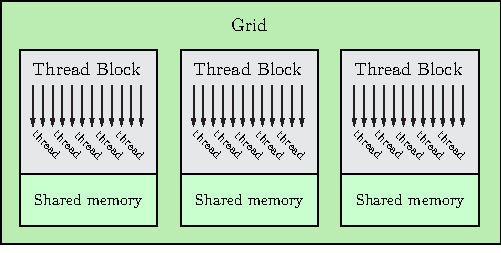
\includegraphics[width=0.8\linewidth]{diagrams/cuda_thread_blocks.pdf}
    \caption{Levels of parallelism granularity. Threads are grouped into thread blocks, which are grouped into conceptual grid. All threads of a thread block have access to its shared memory. }
    \label{fig:cuda-thread block}
\end{figure}

\newcommand{\cuda}[1]{\mintinline{cuda}{#1}}

In Listing \ref{code:Naive saxpy kernel} is demonstrated a simple "saxpy" cuda kernel performing the vector operation $a\vec{x} + \vec{y}$.

\begin{listing}[!ht]
    \caption{Naive saxpy kernel}
    \label{code:Naive saxpy kernel}
\begin{minted}[linenos, escapeinside=!!]{CUDA}
__global__ void saxpy(float* result, float a, const float* x, const float* y)
{
    int i = threadIdx.x;
    result[i] = a*x[i] + y[i];
}

int main()
{
    float* result = ...
    float* x = ...
    float* y = ...
    float a = ...;
    int N = 1000;
    
    saxpy<<<1, N>>>(result, a, x, y);
    assert(cudaGetLastError() == 0);
}
\end{minted}
\end{listing}\FloatBarrier

On line 1 of Listing \ref{code:Naive saxpy kernel}, a kernel is declared using the \cuda{__global__} keyword. Inside of a kernel we have access to built-in variables provided by the execution engine. One of them is \cuda{threadIdx} which denotes the global index of the currently executing thread. For convenient mapping to two or three dimensional problems this index is given as three dimensional vector of type \cuda{dim3}. Because our program is one dimensional, on line 3, we access only its \cuda{x} component to get the index on which to perform computation. On line 4, we perform the parallel computation in the SIMT model. On line 15, we launch the kernel with CUDA launch syntax \cuda{<<<1, N>>>}. The first \emph{launch parameter} (\cuda{1}) is the \emph{grid size}, the number of blocks to launch, the second (\cuda{N}) is \emph{block size}, the number of threads to use for all blocks. These can alternatively be given as type \cuda{dim3} to specify the size in three dimensions. On line 16, we assert that no error occurred using the \cuda{cudaGetLastError()} function. This function returns a standardized error code type \cuda{cudaError_t} whose value of 0 corresponds to no error \cite{CUDA}. We will discuss the variable initialization on lines 9 -- 12, in the subsection \ref{subsection:Cuda memory}.

\subsection{CUDA memory} \label{subsection:Cuda memory}

CUDA divides the memory space available to the program into a few specific types. We will only discuss the ones needed by our implementation. Broadly, memory is split into \emph{host memory} and \emph{device memory}. Here \emph{host} means the CPU issuing kernel launches on one or more CUDA enabled GPU \emph{devices}. As the name implies, \emph{host memory} resides in the hosts RAM while \emph{device memory} resides in device's VRAM (assuming mapped). Data needs to be explicitly allocated and transferred between host and device using specific functions provided by the CUDA runtime. Additionally, \emph{unified memory} can be used, in which case CUDA will transfer data automatically. While unified memory can provide certain advantages related to performance and developer productivity, it is unsuitable for beginner friendly introduction, and thus it will not be discuss further \cite{CUDA}.

\vvskip

In Listing \ref{code:Device memory acquisition}, there is an example of device memory vector initialization to sequence of increasing numbers and subsequent cleanup. Such initialization can be used for all vectors in the "saxpy" Listing \ref{code:Naive saxpy kernel}.

\begin{listing}[!ht]
    \caption{Device memory allocation and deallocation}
    \label{code:Device memory acquisition}
\begin{minted}[linenos]{CUDA}
int main()
{
    int N = 100;
    int size = N * sizeof(float);
    
    float* host_mem = (float*) malloc(size);
    float* device_mem = NULL;
    cudaMalloc(&device_mem, size);

    for(int i = 0; i < N; i++)
        host_mem[i] = i;

    cudaMemcpy(device_mem, host_mem, size, cudaMemcpyHostToDevice);

    //do computation with device_mem

    cudaMemcpy(host_mem, device_mem, size, cudaMemcpyDeviceToHost);
    for(int i = 0; i < N; i++)
        printf("%f\n", host_mem[i]);

    cudaFree(device_mem);
    free(host_mem);
}
\end{minted}
\end{listing}\FloatBarrier

On line 10 of Listing \ref{code:Device memory acquisition}, \cuda{cudaMalloc} is used to obtain \cuda{size} bytes of storage on the device. After the initialization of host memory on lines 10---11, the entire vector is copied to device using \cuda{cudaMemcpy} on line 13. An argument \cuda{cudaMemcpyHostToDevice} is provided to specify the source and destination memory types. 
On line 17 \cuda{cudaMemcpy} is used again to copy device memory back to host. 
Note that all other source and destination memory type combinations in the form \cuda{cudaMemcpy[Source]To[Dest]} can be given. Finally, when the device memory is no longer needed, it is release with a call to \cuda{cudaFree} on line 21. Each of the functions \cuda{cudaMalloc}, \cuda{cudaFree} and \cuda{cudaMemcpy} return a standardized error type \cuda{cudaError_t} \cite{CUDA} which was not checked for brevity. 

\section{Parallel algorithms}\label{sec:parallel algorithms}

We outline all of the algorithms used for efficient implementation of our simulation. Specifically, we need to implement all operations used in Algorithms \ref{alg:Runge-Kutta-Merson method} and \ref{alg:Conjugate Gradient method}.

\subsection{Parallel for} \label{sec:parallel for}

One of the most common operations is executing piece of code over all items of a collection in parallel. We call this parallel for.

In Listing \ref{code:Naive saxpy kernel}, we already saw one way of achieving this effect. A single block was launched with number of threads equal to the number of items $N$. However, since all threads of a single block need to execute on a single SM, their number is limited by the capability of the hardware. Currently, the maximum of threads per block is 1024 for all CUDA devices. Because of this, the saxpy kernel will fail to launch for $N > 1024$. We solve this by introducing the so called \emph{grid stride loop} into our kernel, which will allow us to efficiently execute our kernel for any number of items and any launch parameters. Grid stride loop is shown in Listing \ref{code:Grid stride loop saxpy kernel}.

\begin{listing}[!ht]
    \caption{Grid stride loop saxpy kernel}
    \label{code:Grid stride loop saxpy kernel}
\begin{minted}[linenos]{CUDA}
__global__ void saxpy(float* result, float a, const float* x, const float* y, 
                      int N)
{
    for (int i = blockIdx.x*blockDim.x + threadIdx.x; 
        i < N; 
        i += blockDim.x*gridDim.x) { 
        result[i] = a*x[i] + y[i];
    }
}

int main()
{
    float* result = ...
    float* x = ...
    float* y = ...
    float a = ...;
    int N = 5000;
    
    int blockSize = 256;
    int gridSize = 2; 
    saxpy<<<gridSize, blockSize>>>(result, a, x, y, N);
}
\end{minted}
\end{listing}\FloatBarrier

\cuda{blockIdx}, \cuda{blockDim} and \cuda{gridDim} in Listing \ref{code:Grid stride loop saxpy kernel} are all built-in variables of type \cuda{dim3} similar to \cuda{threadIdx}. \cuda{blockIdx} holds the index of the currently executing block, \cuda{blockDim} holds the block size (here \cuda{blockSize}) and \cuda{gridDim} the number of blocks (here \cuda{gridSize}). On line 3, we convert the provided variables into an index of the worked on item, on line 4, we check if this index is within the bounds of our arrays. This ensures the above code will work even for sizes not necessarily dividable by \cuda{blockSize}. On line 5, we step by the total number of threads in the loop, the so called grid stride. Finally, on line 6, we perform the computation. On line 20, we launch the kernel, providing the number of items \cuda{N}. We are free to choose any block size and grid size.

The grid stride loop results in the following iteration pattern: thread $t_0$ with \cuda{threadIdx}~=~0, \cuda{blockIdx}~=~0 iterates over indices 0, 512, 1024, 1536, \ldots, 4608. Thread $t_1$ with \cuda{threadIdx}~=~1, \cuda{blockIdx}~=~0 iterates over indices 1, 513, 1025, 1537 \ldots 4609. Generally, thread $t_i$ iterates indices 
$\{zBG + i , z = 0,\dots, \floor*{\frac{N}{BG}} \}$ for all $i \in \hat{B}$ 
where $N$ is the number of items, $B$ is block size and $G$ is grid size. This means that threads $t_0$, \ldots, $t_{255}$ always execute on adjacent indices resulting in \emph{coalesced memory accesses}, which is beneficial to the hardware and conceptually simple.

Here we used a common value 256 for block size and arbitrary grid size of 2. Choosing kernel launch parameters is usually done with heuristics. To achieve optimal performance launch parameters grid search or compiler assisted kernel analysis can be used \cite{Jeshani2023CUDA}. However because threads are grouped into \emph{warps}, block size should always be divisible by 32 (see \ref{def:warp}). As there is practically no upper bound to the number of launched blocks, we usually choose grid size to be much larger than are given in Listing \ref{code:Grid stride loop saxpy kernel}. This ensures the block scheduler has sufficient number of concurrently executing blocks to optimally utilize the hardware \cite{CUDA}. For simplicity, we choose grid size such that all threads iterate in the grid size loop only once, that is $G = \ceil*{\frac{N}{B}}$.

We can package the kernel and kernel launch code into a convenient function template, which we will specialize for all desired computations by providing a lambda function. The code is given in Listing~\ref{code:Template parallel for kernel}.

\begin{listing}[!ht]
    \caption{Template parallel for kernel}
    \label{code:Template parallel for kernel}
\begin{minted}[linenos]{CUDA}
template <typename Function>
__global__ void parallel_for_kernel(int from, int N, Function func)
{
    for (int i = blockIdx.x*blockDim.x + threadIdx.x; 
        i < N; 
        i += blockDim.x*gridDim.x) 
        func(from + i);
}

template <typename Function>
void parallel_for(int from, int to, Function func)
{
    int blockSize = 256;
    int gridSize = (to - from + blockSize - 1) / blockSize; //divide round up
    parallel_for_kernel<<<gridSize, blockSize>>>(from, to-from, func);
}

int main()
{
    float* result = ...
    float* x = ...
    float* y = ...
    float a = ...;
    int N = 5000;
    
    parallel_for(0, N, [=]__device__ __host__(int i){
        result[i] = a*x[i] + y[i];
    });
}
\end{minted}
\end{listing}\FloatBarrier

The kernel code on lines 1---8 of Listing \ref{code:Template parallel for kernel}, differs from the grid stride loop in Listing \ref{code:Grid stride loop saxpy kernel} only in by invoking a general code passed in via the \cuda{func} function parameter in place of the previous computation. The launching code on lines 10---16 is using $B = 256$, calculating $G = \ceil*{\frac{N}{B}}$ and passing the arguments into the kernel. Finally, lines 26---28 show calling of the \cuda{parallel_for} function template. A lambda is provided capturing local variable by value (\cuda{[=]}) accepting index \cuda{int i} and performing the computation. A \cuda{__device__ __host__} specifier is applied to the lambda. Similar to the already encountered \cuda{__global__} these specifiers determine how the function is to be called. \cuda{__device__} specifies that the function should only be callable from a device kernel. \cuda{__host__} specifies that the function is only callable from host. This is implicitly added to any function not marked by any of the other specifiers. \cuda{__device__ __host__} together specify that this function can be called from both host and device. Note that a different byte code is generated for the host and device versions of this function. To be able to place these specifiers on lambdas, the code needs to be compiled with \cuda{--extended-lambda} NVCC compiler flag. 

\vvskip

In Listing \ref{code:Two dimensional saxpy kernel}, we present a two dimensional version of the saxpy code with grid stride loop \ref{code:Grid stride loop saxpy kernel}. The transformation from one dimensional to two dimensional code is relatively straightforward and as such we will only present one dimensional variants from now on. We can also wrap this code in a generic wrapper similar to Listing \ref{code:Template parallel for kernel} to obtain \cuda{parallel_for_2D}.

\begin{listing}[!ht]
    \caption{Two dimensional saxpy kernel}
    \label{code:Two dimensional saxpy kernel}
\begin{minted}[linenos]{CUDA}
__global__ void saxpy2D(float* result, float a, const float* x, const float* y, 
                        int N, int M)
{
    for (int i = blockIdx.y*blockDim.y + threadIdx.y; 
        i < M; i += blockDim.y*gridDim.y) 
        for (int j = blockIdx.x*blockDim.x + threadIdx.x; 
            j < N; j += blockDim.x*gridDim.x) 
        {
            int I = i*N + j;
            result[I] = a*x[I] + y[I];
        }
}

int main()
{
    float* result = ...
    float* x = ...
    float* y = ...
    float a = ...;
    int N = 1000;
    int M = 3000;
    
    dim3 blockDim(16, 16);
    dim3 gridDim(4, 4);
    saxpy2D<<<gridDim, blockDim>>>(result, a, x, y, N, M);
}
\end{minted}
\end{listing}\FloatBarrier

\subsection{Parallel tiled for}

The parallel for given in Listing \ref{code:Template parallel for kernel} can be used for a majority of the needed operations, including a specialized version of matrix multiplication for matrices in the form (\ref{eq:Semi-Implicit matrices}) with a nonzero diagonal and four nonzero off diagonals. For now, let us consider a simpler case of a tridiagonal matrix $\mat{A} \in \R^{N \times N}$ such that $\forall i \in \hat{N}$ \label{def:tridiagonal matrix example}
\begin{align}
    \mat{A}_{i,j} = \begin{cases}
            a \text{ when $i = j$}, \\
            b \text{ when $i = j-1$}, \\
            c \text{ when $i = j+1$}, \\
            0 \text{ otherwise} \\
        \end{cases}
\end{align}
for some constants $a$, $b$, $c \in \R$. Consider the multiplication of vector $\vec{x} \in \R^N$ by matrix $\mat{A}$ \label{eq:tridiagonal multiplication}
\begin{align}
    (\mat{A}\vec{x})_i = bx_{i-1} + ax_i + cx_{i+1}
\end{align}
$\forall i \in \{1, \ldots, N-1\}$. Using \cuda{parallel_for}, this can be turned into a CUDA function in Listing \ref{code:Naive tridiagonal matrix multiplication kernel}. 
\begin{listing}[!ht]
    \caption{Naive tridiagonal matrix multiplication kernel}
    \label{code:Naive tridiagonal matrix multiplication kernel}
\begin{minted}[linenos]{CUDA}
void tridiag_mul(float* result, float a, float b, float c, const float* x, int N)
{
    parallel_for(1, N-1, [=]__device__ __host__(int i){
        result[i] = b*x[i-1] + a*x[i] + c*x[i+1];
    });  
}
\end{minted}
\end{listing}\FloatBarrier
We will refer to device memory obtained by calling \cuda{cudaMalloc} or similar as \emph{global memory}. 
The kernel in Listing \ref{code:Naive tridiagonal matrix multiplication kernel} perform 3 global memory reads, three multiplies and two additions for each item. As the computation performed is fast in comparison to the global memory latency, the scheduler is not able schedule useful work while the threads are waiting for the memory reads to complete. Thus most of the kernel execution time is spend idly waiting for data. If we consider the case of matrix in the form (\ref{def:tridiagonal matrix example}) with 5 nonzero diagonals and matrix coefficients that vary by row, this effect is even more pronounced. 10 global memory reads are required per processed element.

We eliminate some of these reads if we consider that neighbouring output elements read mostly the same values. That is for example in the tridiagonal matrix multiplication (\ref{eq:tridiagonal multiplication}) both output elements $(A\vec{x})i$,$(A\vec{x})_{i+1}$ read $x_i$ and $x_{i+1}$. We utilize \emph{shared memory}, which is shared between all threads of a single thread block, to efficiently broadcast values between neighbouring threads. All of the needed input values for the entire block are loaded into shared memory, then each thread executes its operation reading only from shared memory, which is expected to be much faster.

\begin{figure}[!ht]
    \centering
    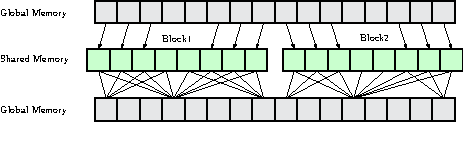
\includegraphics[width=0.8\linewidth]{diagrams/cuda_shared_mem.pdf}
    \caption{A graphic depicting usage of shared memory. Data is read from global memory (top) into per block shared memory (middle), computation is performed and results are stored back into global memory (bottom).}
    \label{fig:shared memory}
\end{figure}

First, let us introduce programming with shared memory. A variable declared with memory space specifier \cuda{__shared__} is allocated in shared memory. Such a variable is accessible to all threads of a particular thread block. Because of this, any access to it needs to be handled with extra care to prevent data races. In the case of a single variable atomic operations need to be used. In case of an array, each thread of a thread block must write to a different index. When reading from shared memory which was updated by another thread, thread synchronization is required to ensure all threads have completed their update. This is done using the \cuda{__syncthreads()} builtin function, which halts execution of the calling thread until all threads in its thread block reached this function call \cite{CUDA}.

\vvskip

In Listing \ref{code:Sum 64 items kernel} is an example kernel that sums "tiles" of 64 neighbouring items using shared memory. Notice that only one global memory read per output element is required instead of 64 if shared memory was not used.
\begin{listing}[!ht]
    \caption{Sum 64 items kernel}
    \label{code:Sum 64 items kernel}
\begin{minted}[linenos]{CUDA}
__global__ void sum64(float* result, const float* x, int N)
{
    assert(blockDim.x == 64);
    __shared__ float shared[64];
    
    int i = blockIdx.x*blockDim.x + threadIdx.x;
    shared[threadIdx.x] = x[i];
    __syncthreads();

    float sum = 0;
    for(int j = 0; j < 64; j++)
        sum += shared[j];

    result[i] = sum;
}

int main()
{
    float* result = ...
    float* x = ...
    int N = 1024;
    
    sum64<<<N/64, 64>>>(result, x, N);
}
\end{minted}
\end{listing}\FloatBarrier

On line 4 of Listing \ref{code:Sum 64 items kernel}, array in shared memory is declared. On line 6, an index into global memory is calculated and used to load values into shared memory on line 7. Notice that \cuda{threadIdx.x} is used to index into \cuda{shared} as shared memory is unique on per block basis. On line 8, \cuda{__syncthreads()} is called to ensure all threads have finished loading values into \cuda{shared} and thus these values are safe to read. On lines 10---14, sum of the items in the "tile" are calculated and output into \cuda{result}. The launch code on lines 17---25 remains in its usual form. Note that $N$ needs to divisible by 64. Otherwise, the code will read outside of the provided arrays in global memory.

Next, we extend the code in Listing \ref{code:Sum 64 items kernel} above so that $N$ can be of any value and the "tile size" (previously 64) can be set dynamically. For this, we need to obtain a dynamic amount of shared memory. This requires a new syntax and new launch parameter as shown in Listing \ref{code:Sum tile kernel}.

\begin{listing}[!ht]
    \caption{Sum tile kernel for general value of $N$}
    \label{code:Sum tile kernel}
\begin{minted}[linenos]{CUDA}
__global__ void sum_tile(float* result, const float* x, int N)
{
    extern __shared__ float shared[];
    for (int i_base = blockIdx.x*blockDim.x; ; i_base += gridDim.x*blockDim.x) 
    {
        if(i_base >= N)
            break;
            
        int i = i_base + threadIdx.x;
        float read = 0;
        if(i < N)
            read = x[i];

        shared[threadIdx.x] = read;
        __syncthreads();

        if(i < N)
        {
            float sum = 0;
            for(int j = 0; j < blockDim.x; j++)
                sum += shared[j];
    
            result[i] = sum;
        }
        __syncthreads();
    }
}

int main()
{
    float* result = ...
    float* x = ...
    int N = 5000;
    int tileSize = 700;
    
    int blockSize = tileSize;
    int gridSize = (N + blockSize - 1)/blockSize;
    int sharedMemSize = blockSize*sizeof(float);
    sum_tile<<<gridSize, blockSize, sharedMemSize>>>(result, x, N);
}
\end{minted}
\end{listing}\FloatBarrier

On line 3 of Listing \ref{code:Sum tile kernel}, we used a different syntax to obtain dynamically sized array in shared memory. On lines 4---7, we used grid stride loop to handle arbitrary sizes. All threads of a given thread block need to execute \cuda{__syncthreads()}, else a deadlock would occur. Because of this, extra care needs to be taken around the stop condition, which needs to evaluate the same for all threads within a thread block. On lines 9---15, we load values into shared memory. This time, we only read values out of global memory if the thread's output index is inside the given array, else we load value 0. This ensures the whole \cuda{shared} array is initialized. Next, on lines 17---24, we perform the computation on threads whose output index is within the array. Then, on line 25, we synchronize one last time. This ensures no thread starts executing the next iteration overriding values in the \cuda{shared} array while computation is still in progress. Finally, on lines 36---39, we launch the kernel. \cuda{blockSize} is set to the size of the tile (max 1024) and \cuda{gridSize} is set according to $G = \ceil*{\frac{N}{B}}$. The needed shared memory size per block \cuda{sharedMemSize} is calculated and given as a third launch parameter. This specifies the amount of memory to be allocated for the \cuda{shared} array.

Note that shared memory per block is a limited resource usually in tens of kilobytes on a typical CUDA enabled GPU. Devices of the NVIDIA Hopper architecture have up to 227~KB available shared memory per block \cite{CUDA}. For the kernel in Listing \ref{code:Sum tile kernel} operating on \cuda{float}, supplying maximum block size $B = 1024$ results in 4KB shared memory used. While not a concern here, shared memory usage is another factor affecting possible range of launch parameters.

\vvskip 

We are ready to present the kernel for the tridiagonal matrix multiplication in Listing \ref{code:Tridiagonal matrix multiplication kernel}. Because each thread with output index $i$ reads values at indices $i-1$, $i$, $i+1$, we only execute the computation on threads in the interior of the thread block. More generally only for threads $t_r$, \ldots, $t_{B-r-1}$, where $r$ is the "radius", ie., distance between the index $i$ and furthest index read by the thread with output index $i$. Here $r = 1$. 

\begin{listing}[!ht]
    \caption{Tridiagonal matrix multiplication kernel}
    \label{code:Tridiagonal matrix multiplication kernel}
\begin{minted}[linenos]{CUDA}
__global__ void tridiag_mul_shared(float* result, float a, float b, float c, 
                                   const float* x, int N)
{
    extern __shared__ float shared[];

    int r = 1;
    int ti = threadIdx.x;
    for (int bi = blockIdx.x; ; bi += gridDim.x) 
    {
        int i_base = bi*blockDim.x - 2*bi*r;
        if(i_base >= N)
            break;

        int i = i_base - r + ti;
        float val = 0;

        if(0 <= i && i < N)
            val = x[i];

        shared[ti] = val;
        __syncthreads();

        if(r <= ti && ti < blockDim.x-r && i < N)
            result[i] = b*shared[ti-1] + a*shared[ti] + c*shared[ti+1];
            
        __syncthreads();
    }
}
\end{minted}
\end{listing}\FloatBarrier

The code in Listing \ref{code:Tridiagonal matrix multiplication kernel} can be extended to two dimensions similar to parallel for in Listing \ref{code:Template parallel for kernel}. By templating this function over type \cuda{T} of the \cuda{shared} array and replacing lines 13---15 and 22 by an invocation of a function passed to the kernel, we can generalize this algorithm to be used in all scenarios necessary by the implementation. The resulting function template signature is shown in Listing \ref{code:Templated tiled for kernel declaration}. \cuda{gather} loads or produces data stored into shared memory and \cuda{func} performs the computation utilizing shared memory. For full, implementation see the \href{https://github.com/Boostibot/bachelors/tree/72edc68ca91fca5fd0abf40726ea415c6e932e5d}{project repository}.

\begin{listing}[!ht]
    \caption{Templated tiled for kernel declaration}
    \label{code:Templated tiled for kernel declaration}
\begin{minted}[linenos]{CUDA}
template <int r, typename T, typename Function, typename Gather>
void tiled_for(int from, int to, Gather gather, Function func);

//Gather and Function are expected to have signatures (pseudocode):
T gather(int i, int N, int r);
void func(int i, int sharedIdx, int tileSize, cont T* shared); 
\end{minted}
\end{listing}\FloatBarrier

\subsection{Parallel reduction}\label{sec:parallel reduction}
Last algorithm needed for efficient implementation of our simulation is the parallel reduction. This operation consists in repeatedly applying a reduction operator $v$ to array of values until only one value is left. More formally, let $T$ be a set of possible values of some type. Let $v:T\times T \to T$ be an operator that is associative, commutative and has identity element $e$ ie., $v(e,x)=x \forall x\in T$. Then reduction is a function $R:T^N \to~T:\vec{x}~\mapsto~v(v(...v(v(e, x_1), x_2), ...), x_n)$, for some $N \in \Nats$. Some examples of common used reduction operators include $+$, $\min$ and $\max$. We also use reduction to implement dot product and various vector norms.

Note that some implementations require $v$ to be only commutative. However, we will need all three properties listed. For the sake of simplicity, we will be using the $\max$ reduction operator with identity value $-\infty$ in all further discussions.

A serial implementation of reduction using $\max$ reduction operator, is shown in Listing \ref{code:Serial reduction}.
\begin{listing}[!ht]false
    \caption{Serial reduction}
    \label{code:Serial reduction}
\begin{minted}[linenos]{CUDA}
float reduce(const float* x, int N)
{
    float max = -INFINITY;
    for(int i = 0; i < N; i++)
        max = fmaxf(max, x[i]);
        
    return max;
}
\end{minted}
\end{listing}\FloatBarrier
Of course, we want to perform this operation in parallel. The first key idea is "folding". In each iteration, we divide the remaining array in half and perform parallel reduction of the first and second half. This shrinks the remaining array to half of its original size (given that its size was even). We stop when the remaining size is just one item. This operation needs $\ceil*{\log_2(N)}$ iterations each involving a separate kernel launch. The code is given in Listing \ref{code:Reduction in global memory}. 

\begin{listing}[!ht]
    \caption{Reduction in global memory}
    \label{code:Reduction in global memory}
\begin{minted}[linenos]{CUDA}
float global_mem_reduce(float* temp1, float* temp2, const float* x, int N)
{
    cudaMemcpy(temp1, x, N*sizeof(float), cudaMemcpyDeviceToDevice);
    while(N > 1)
    {
        int half = (N + 1) / 2;
        parallel_for(0, half, [=]__device__ __host__ (int i){
            if(i + half < N)
                temp2[i] = fmaxf(temp1[i], temp1[i + half]);
            else
                temp2[i] = temp1[i];
        });  

        std::swap(temp1, temp2);
        N = half;
    }

    float max = -INFINITY;
    cudaMemcpy(&max, temp1, sizeof(float), cudaMemcpyDeviceToHost);
    return max;
}
\end{minted}
\end{listing}\FloatBarrier

We can optimize the number of kernel launches and accesses to global memory by utilizing shared memory. First, we perform partial reduction in global memory until only $G$ items remain, where G is the grid size (see Section \ref{sec:parallel for}). Then a per block reduction is performed utilizing shared memory. The per block reduction result is written into a smaller output array. This yields a single value per block stored in global memory. The remaining $G$ items are either reduced by invoking the kernel again or are reduced on the CPU if $G$ is small. For problem sizes encountered by our simulation, this process yields one or two kernel launches depending on the choice of $G$. The resulting code is given in Listing \ref{code:Reduction in shared memory}. Additionally an optimization on the kernel launching code has been performed eliminating one \cuda{cudaMemcpy} call. 

\begin{listing}[!ht]
    \caption{Reduction in shared memory}
    \label{code:Reduction in shared memory}
\begin{minted}[linenos,fontsize=\small]{CUDA}
__global__ void shared_mem_reduce_kernel(float* output, const float* input, int N) 
{
    assert((blockDim.x & (blockDim.x-1)) == 0 && "must be power of two!");
    extern __shared__ float shared[];

    int ti = threadIdx.x;
    float reduced = -INFINITY;
    for(int i = blockIdx.x*blockDim.x + ti; 
        i < N; i += blockDim.x*gridDim.x)
        reduced = fmaxf(input[i], -INFINITY);

    shared[ti] = reduced;
    __syncthreads();
    
    for(int sharedSize = blockDim.x/2; sharedSize > 0; sharedSize /= 2) {
        if(ti < sharedSize)
            shared[ti] = fmaxf(shared[ti], shared[ti + sharedSize]);
        __syncthreads();      
    } 

    if(ti == 0)
        output[blockIdx.x] = shared[0];
}

float shared_mem_reduce(float* temp1, float* temp2, const float* input, int N)
{
    const float* from = input;
    enum {MIN_SIZE = 64};
    while(N > MIN_SIZE) {
        int blockSize = 1024;
        int sharedMemSize = blockSize*sizeof(float);
        int gridSize = (N + blockSize - 1) / blockSize;

        shared_mem_reduce_kernel
            <<<gridSize, blockSize, sharedMemSize>>>(temp2, from, N);

        std::swap(temp1, temp2);
        N = gridSize;
        from = temp1;
    }
    float cpu[MIN_SIZE] = {0};
    cudaMemcpy(cpu, from, N*sizeof(float), cudaMemcpyDeviceToHost);
    
    float max = -INFINITY;
    for(int i = 0; i < N; i++)
        max = fmaxf(max, cpu[i]);
    return max;
}
\end{minted}
\end{listing}\FloatBarrier

We can optimize this implementation in Listing \ref{code:Reduction in shared memory} further by utilizing \emph{warps} \label{def:warp} which are collections of 32 threads. The CUDA processor creates, executes and schedules threads only on per warp basis. Prior to the NVIDIA Volta architecture, all threads in a single warp shared the same program counter. That is, all threads of a warp executed the same instructions similarly to SIMD (Single Instruction Multiple Data) programming. This also meant that the CUDA processors were unable to execute conditional \cuda{if}/\cuda{else} branches unless the condition evaluated the same for all threads in a warp. In those cases, the processor would execute both the \cuda{if} and \cuda{else} code block for all threads in a warp, but only store the computation result for the \emph{active threads}, that is threads, for which the condition evaluated according to the currently executed branch. This process is called \emph{warp divergence} and is undesired because of its sub-optimal performance. NVIDIA Volta architectures and later eliminate warp divergence by providing full concurrency between threads independent of warp. Each thread has its own program counter and is able to be scheduled independently. Still, warps play an important role as they allow efficient thread communication within a single warp \cite{CUDA}.

\vvskip

We use warp communication to share partial reduction results similarly to shared memory in Listing \ref{code:Reduction in shared memory}. First, partial reduction in global memory is performed until only $B$ items per block remain. Then a warp level reduction is performed, yielding a value which is stored into shared memory and all threads of a block are synchronized. The first $B/32$ threads of a block load values from shared memory and perform warp level reduction again. This time the resulting $B/32^2$ values are stored into global output memory. With $B \le 1024$ this yields a single value per block stored in global memory. Similarly to reduction in shared memory, the partial reduction results are reduced by a repeated kernel launch or are processed on the CPU. The resulting code is given in Listing \ref{code:Reduction using warp instructions}. 

\begin{listing}[!ht]
    \caption{Reduction using warp instructions}
    \label{code:Reduction using warp instructions}
\begin{minted}[linenos]{CUDA}
__global__ void warp_reduce_kernel(float* output, const float* x, int N) 
{
    enum {WARP_SIZE = 32};
    assert(blockDim.x > WARP_SIZE && blockDim.x % WARP_SIZE == 0);

    extern __shared__ float shared[];
    uint shared_size = blockDim.x / WARP_SIZE;

    float reduced = 0;
    for(int i = blockIdx.x*blockDim.x + threadIdx.x; i < N; i += blockDim.x*gridDim.x)
        reduced = fmaxf(reduced, x[i]);

    for (int offset = WARP_SIZE / 2; offset > 0; offset /= 2) 
        reduced = fmaxf(__shfl_down_sync(0xffffffffU, reduced, offset), reduced);

    uint ti = threadIdx.x;
    if (ti % WARP_SIZE == 0) 
        shared[ti / WARP_SIZE] = reduced;
    
    __syncthreads();
    uint ballot_mask = __ballot_sync(0xffffffffU, ti < shared_size);
    if (ti < shared_size) 
    {
        reduced = shared[ti];
        for (int offset = WARP_SIZE / 2; offset > 0; offset /= 2) 
            reduced = fmaxf(__shfl_down_sync(ballot_mask, reduced, offset), reduced);
    }

    if (ti == 0) 
        output[blockIdx.x] = reduced;
}

//same as shared_mem_reduce but calls warp_reduce_kernel
float warp_reduce(float* temp1, float* temp2, const float* input, int N);
\end{minted}
\end{listing}\FloatBarrier

Like in the parallel algorithms already discussed, we template the reduction kernel in Listing \ref{code:Reduction using warp instructions} over the specific type and reduction operator used. Additionally we provide "producer" lambda which abstracts the retrieval of reduced values. This creates the so called map-reduce operation, which can be used to efficiently implement many vector operations such as the Euclid norm shown is Listing \ref{code:Template reduction}.
Note that the implementation requires both reduction function and its identity element which are provided via the functor type \cuda{Reduction}. While custom reduction operators can be defined, the common operators are provided. This allows the implementation to use warp level reduction intrinsics where eligible. These intrinsics replace the lines 13---14 and 25---26 in Listing \ref{code:Reduction using warp instructions} and are expected to be much faster. An example of such intrinsic for the \cuda{int} type and add reduction operator is \cuda{__reduce_add_sync} \cite{CUDA}. 

\begin{listing}[!ht]
    \caption{Template reduction}
    \label{code:Template reduction}
\begin{minted}[linenos]{CUDA}
template <typename T, class Reduction, typename Producer>
T produce_reduce(int N, Producer produce, int cpu_reduce = 256);

float euclid_norm(const float *a, int N)
{
    float output = produce_reduce<float, Reduce::Add>(N, 
        [=]__host__ __device__(int i){
            return a[i]*a[i];
        });
    return sqrtf(output);
}
\end{minted}
\end{listing}\FloatBarrier

\section{Algorithm benchmarks}\label{sec:algorithm benchmarks}
We try to measure the speed of the proposed algorithms in Section \ref{sec:parallel algorithms}. Due to time constraints, only the parallel reduction algorithm given in Section \ref{sec:parallel reduction} is measured.

The benchmark procedure consists of the following steps: firstly, an array of size $N \in \Nats$ filled with pseudo-random values is generated. This array is used as the input to the benchmarked algorithm. Then, the algorithm is run repeatedly for $t_\text{warmup}$ seconds. This ensures all relevant data is cached. Next, the algorithm is run for $t_\text{measure}$ seconds, measuring and storing its execution time. Additionally, if more then $N_\text{samples}$ running times are collected, the benchmark is stopped. Finally, the running process is put to sleep for $t_\text{cooldown}$, ensuring no heat throttling occurs. We report the median running time of the samples collected.

We benchmarked the parallel reduction algorithm given in Section \ref{sec:parallel reduction}, CUDA Thrust library \cuda{thrust::reduce} and naive serial reduction given in Listing \ref{code:Serial reduction}. The algorithms use the $\max$ reduction operator on the \cuda{float} data type.

The benchmarking procedure was run repeatedly for multiple input sizes \\$N \in \{256^2, 512^2, 1024^2, 2048^2, 4096^2, 2\times4096^2\}$ and  parameters $t_\text{warmup} = 0.3$, $t_\text{measure} = 3$, $t_\text{cooldown} = 5$, $N_\text{samples} = 1024^2$. 

The benchmark was run on a laptop using Ubuntu 22.04.4 LTS, NVIDIA GeForce MX450, Driver Version: 535.183.01, CUDA Version: 12.2, 11th Gen Intel(R) Core(TM) i5-1135G7 @ 2.40GHz.

It is worth noting that the benchmarking procedure never collected more than $N_\text{samples}$ thus the benchmark run for the full $t_\text{measure}$ duration. The results are summarized in Table \ref{tab:benchmark results} and Figure \ref{fig:benchmark results}. The full benchmarking code implementation can be found in the \href{https://github.com/Boostibot/bachelors/tree/72edc68ca91fca5fd0abf40726ea415c6e932e5d}{project repository}.

\FloatBarrier
\begin{figure}[!ht]
    \centering
    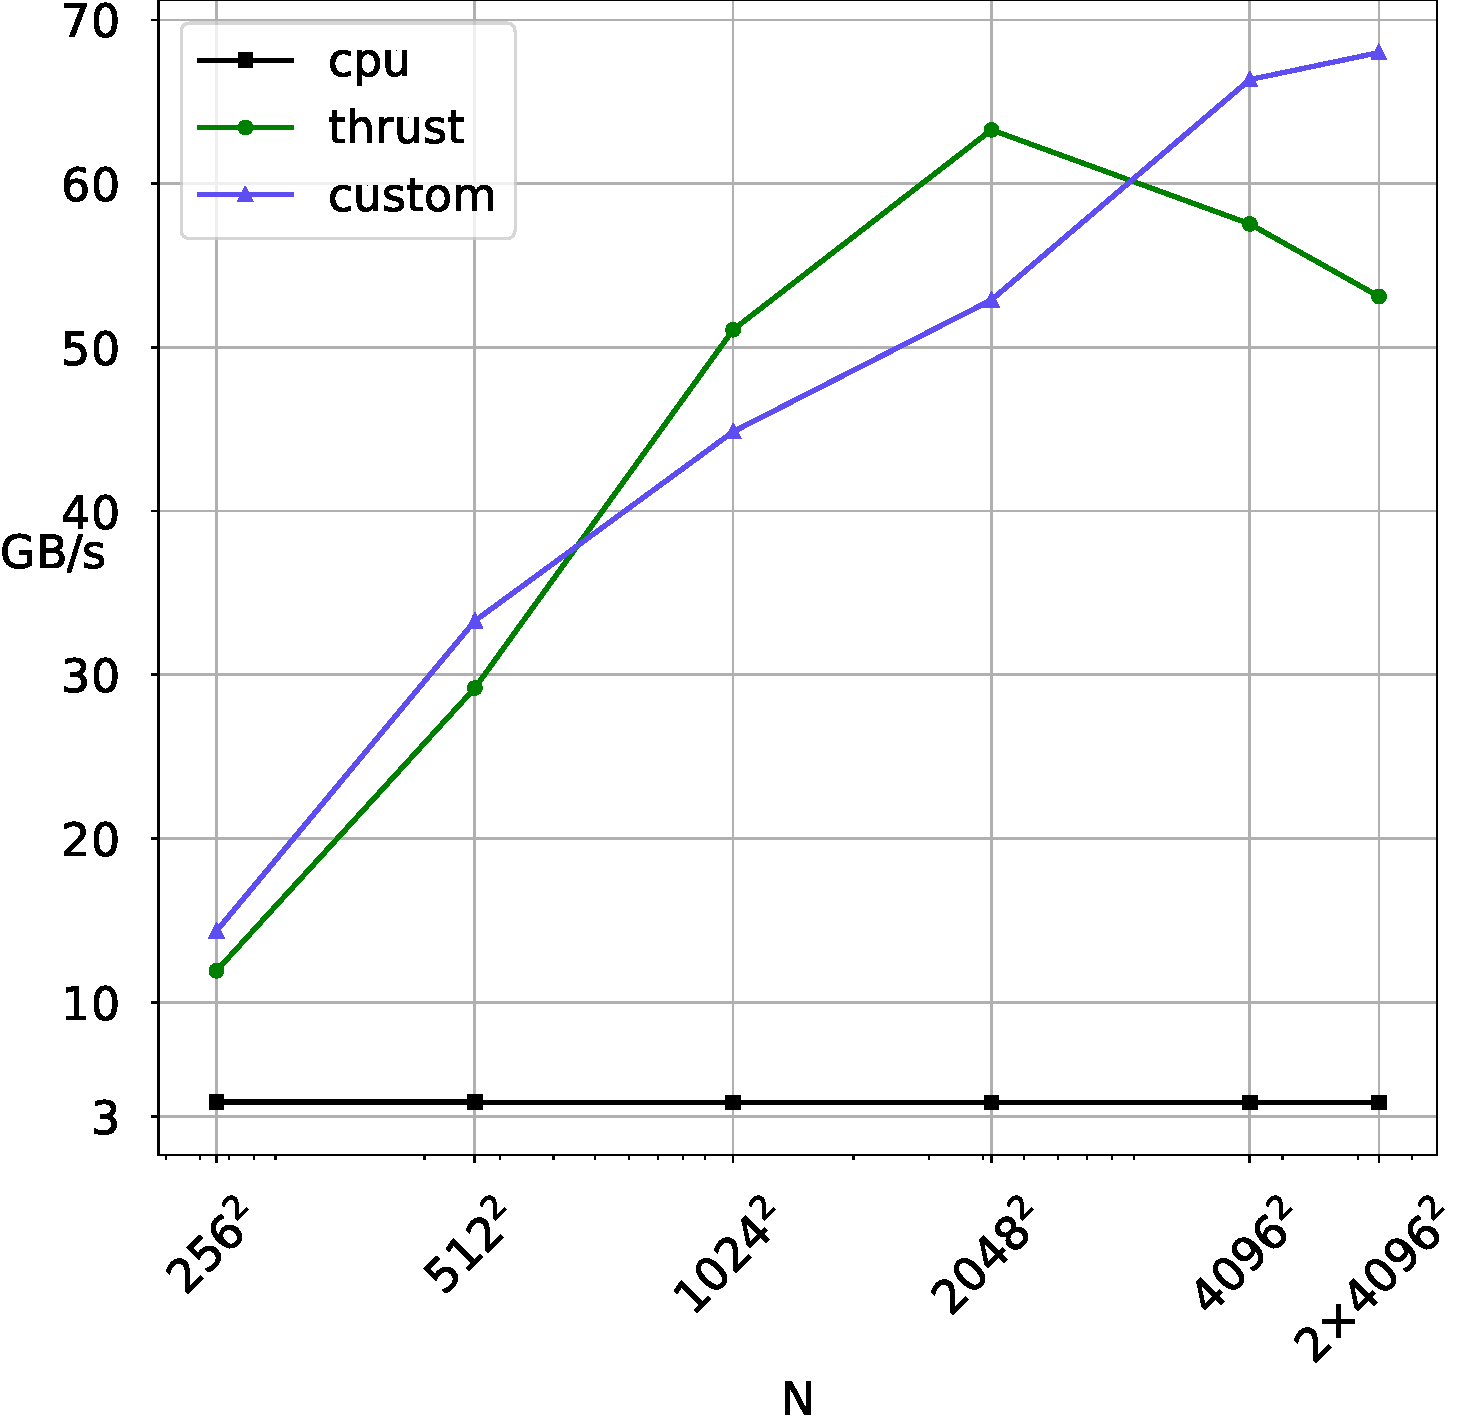
\includegraphics[width=0.8\linewidth]{results/benchmark.pdf}
    \caption{Median running times of the benchmarked reduction algorithms expressed in gigabytes of processed data per second. On the $x$ logarithmic axis is the size of the dataset $N$.}
    \label{fig:benchmark results}
\end{figure}

\FloatBarrier
\begin{table}[!ht]
    \centering
    \begin{tabular}{|l|l|l|l|l|l|l|}
        \hline
        & & & & & & \\[-1em]
        N & $256^2$ & $512^2$ & $1024^2$ & $2048^2$ & $4096^2$ & $2\times4096^2$ \\
        \hline
        & & & & & & \\[-1em]
        cpu    & $6.26\times 10^{-5}$ & $2.50\times 10^{-4}$ & $1.01\times 10^{-3}$ & $4.04\times 10^{-3}$ & $1.61\times 10^{-2}$ & $3.22\times 10^{-2}$ \\
        \hline
        & & & & & & \\[-1em]
        thrust & $2.05\times 10^{-5}$ & $3.34\times 10^{-5}$ & $7.65\times 10^{-5}$ & $2.47\times 10^{-4}$ & $1.09\times 10^{-3}$ & $2.35\times 10^{-3}$ \\
        \hline
        & & & & & & \\[-1em]
        custom & $1.70\times 10^{-5}$ & $2.93\times 10^{-5}$ & $8.71\times 10^{-5}$ & $2.95\times 10^{-4}$ & $9.42\times 10^{-4}$ & $1.84\times 10^{-3}$ \\
        \hline
    \end{tabular}
    \caption{Median running times in seconds of the benchmarked reduction algorithms.}
    \label{tab:benchmark results}
\end{table}
\FloatBarrier

From the collected results in Table \ref{tab:benchmark results} and Figure \ref{fig:benchmark results}, we conclude that the parallel reduction algorithm given in Section \ref{sec:parallel reduction}, outperforms the implementation in the Thrust library for small and large input sizes sizes on the used hardware. However, for input sizes of $N = 1024^2, 2048^2$ the Thrust implementation achieves considerably shorter running times.

% \pagestyle{headings}

% \pagestyle{headings}
\chapter{Results} \label{chap:results}

We present and discuss the results obtained by running the algorithm developed by using the techniques in Chapter \ref{chap:time integration schemes} in various settings.
First, we explore the impact of different simulation parameters on resulting crystal structures. Then, comparison between different integration methods is performed. Finally, the effect of repeated time stepping and correction term is quantified (see Sections \ref{sec:repeated time stepping} and \ref{sec:correction term}). 
\section{Parameter setting}


\subsection{Boundary conditions} \label{sec:simulation boundary conditions}

For the temperature field $T$ the homogeneous Dirichlet boundary condition (see Section \ref{sec: Dirichlet boundary condtions}) written as 
\begin{align}
    T|_{\partial \Domain} = 0 \text{ on } \Timeint \times \partial \Omega \label{eq:dirichlet T boundary conditions},
\end{align} which can be interpreted a controlled cooling so that $\partial \Domain$ is kept at constant temperature. The temperature in the domain $\Omega$ approaches 0. This results in unbounded growth of the crystal which eventually fills the whole domain $\Domain$. This process is shown in Figure \ref{fig:s-i filling}.

The homogeneous Neumann boundary condition (see Section \ref{sec: Neumann boundary condtions}) written as 
\begin{align}
    \nabla T \cdot \vec{n} = 0 \text{ on } \Timeint \times \partial \Omega \label{eq:def T boundary conditions},
\end{align} means the system is adiabatically isolated. No heat is transferred across the boundary $\partial \Domain$. As the system approaches thermodynamic equilibrium, it minimizes its interfacial energy, making the crystal structure more rounded in a process called \emph{coarsening}. The crystal in limit approaches the so called \emph{Wulff shape} \cite{StrachotaDizertation}, \cite{Gurtin93WulfShape}. This process is shown in Figure \ref{fig:s-i coarsening}.
% We will use the homogeneous Neumann boundary condition in further result unless stated otherwise.

For the phase filed $\Phi$, the homogeneous Dirichlet boundary condition
\begin{align}
    \Phi|_{\partial \Domain} = 0 \text{ on } \Timeint \times \partial \Omega
\end{align}
represents an unrealistic jump change from the crystal structure in the domain $\Domain$ to perfect liquid phase on the boundary $\partial \Domain$. This creates high phase field flux for crystal structures near the boundary, which through the latent heat $L$ term rapidly cools the surroundings, prompting spurious crystal growth. On the other hand, for $\Phi$ the homogeneous Neumann boundary condition 
\begin{align}
    \nabla \Phi \cdot \vec{n} = 0 \text{ on } \Timeint \times \partial \Omega \label{eq:def Phi boundary conditions}
\end{align}
allows the crystal to reach the boundary but does not cause spurious crystal growth. Because of this the homogeneous Neumann boundary condition is used in all subsequent simulations.

\subsection{Initial conditions} \label{sec:setup initial conditions}
Initial conditions are specified to conform to the modeled process of solidification in an under-cooled medium. The temperature is uniformly initialized below the melting point
\begin{align}
    T_{ini}(\vec{x}) = 0 && \forall \vec{x} \in \Domain \label{eq:def T initial conditions}
\end{align}
and the phase is initialized to liquid phase except for initial nucleus of solid phase 
\begin{align}
    \Phi_{ini}(\vec{x}) = \begin{cases} \label{eq:def Phi initial conditions}
        1 & \text{ when } \hphantom{R_{ini} + \xi_0/2 < } d(\vec{x}) < R_{ini} - \xi_0/2,  \\
        1 - \bigfrac{d(\vec{x}) - R_{ini} + \xi_0/2}{\xi_0} & \text{ when } R_{ini} + \xi_0/2 < d(\vec{x}) < R_{ini} - \xi_0/2,\\
        0 & \text{ when } R_{ini} + \xi_0/2 \le d(\vec{x}),
    \end{cases} && \forall \vec{x} \in \Domain,
\end{align}
where $d(\vec{x}) = |\vec{x} - \vec{x}_0|$ is the distance to the nucleus center $\vec{x}_0$ and $R_{ini} \in \R$ is the nucleus radius \cite{StrachotaDizertation}. $\xi_0 \in \R$ determines the size of linear transition between the solid and liquid phase. The value of $\xi_0$ is chosen so that the initial condition better approximates the shape of the phase interface (see Figure \ref{fig:phase interface result}). While even with $\xi_0 = 0$ the interface quickly develops to the expected shape, properly chosen $\xi_0$ helps to reduce sudden changes in temperature and phase fields near the start of the simulation, which could cause the employed schemes to diverge. This effect can be observed in Figure \ref{fig:step res comp}.

\subsection{Simulation setup} \label{sec:simulation setup}
% We specify model parameters, boundary and initial conditions used in the subsequent simulations. 

 Homogeneous Neumann boundary conditions are used for both the temperature and the phase field. Initial conditions given by (\ref{eq:def Phi boundary conditions}) and (\ref{eq:def Phi initial conditions}) are used with $\vec{x}_0 = (2,2)$, $ R_{ini} = 0.04$, $\xi_0 = 8\xi$. The model parameters are summarized in the Table \ref{tab:model parameters}. 
 
 For the RKM scheme given in Section \ref{sec: explicit scheme}, tolerance $\varepsilon = 5\times10^{-3}$ is used. For the S-I scheme given in Section \ref{sec: semi implicit scheme}, coefficient $\gamma = 1$ and tolerance $\varepsilon = 5\times10^{-9}$ are used. 

\vvskip
\FloatBarrier
\begin{table}[!ht]
    \centering
    % {
    % \setstretch{1.1}
    \begin{tabular}{ll} 
        \toprule
        $\Omega = (0, 4)\times(0, 4)$ & $\Timeint = [0, 0.04]$ \\
        $n_x = n_y = 1024$ & $\dt = 5\times10^{-5}$ \\
        $\dx = \dy = 4/1024$ & $\xi = 0.0043$ \\
        $a = 2$ & $\alpha = 3$ \\
        $b = 1$ & $\beta = 1400$ \\
        $L = 2$ & $T^* = 1$ \\
        $S = 0.3$ & $m = 6$ \\
        $\theta_0 = 0$ & \\
        \bottomrule
    \end{tabular}
    % }
    \caption{Simulation model parameters}
    \label{tab:model parameters}
\end{table}
\FloatBarrier


\setlength{\subfigwidth}{0.31\textwidth}
\FloatBarrier
\begin{figure}[!ht]
\centering
\begin{tabular}{P{\subfigwidth}P{\subfigwidth}P{\subfigwidth}}

\raisebox{-0.5\height}{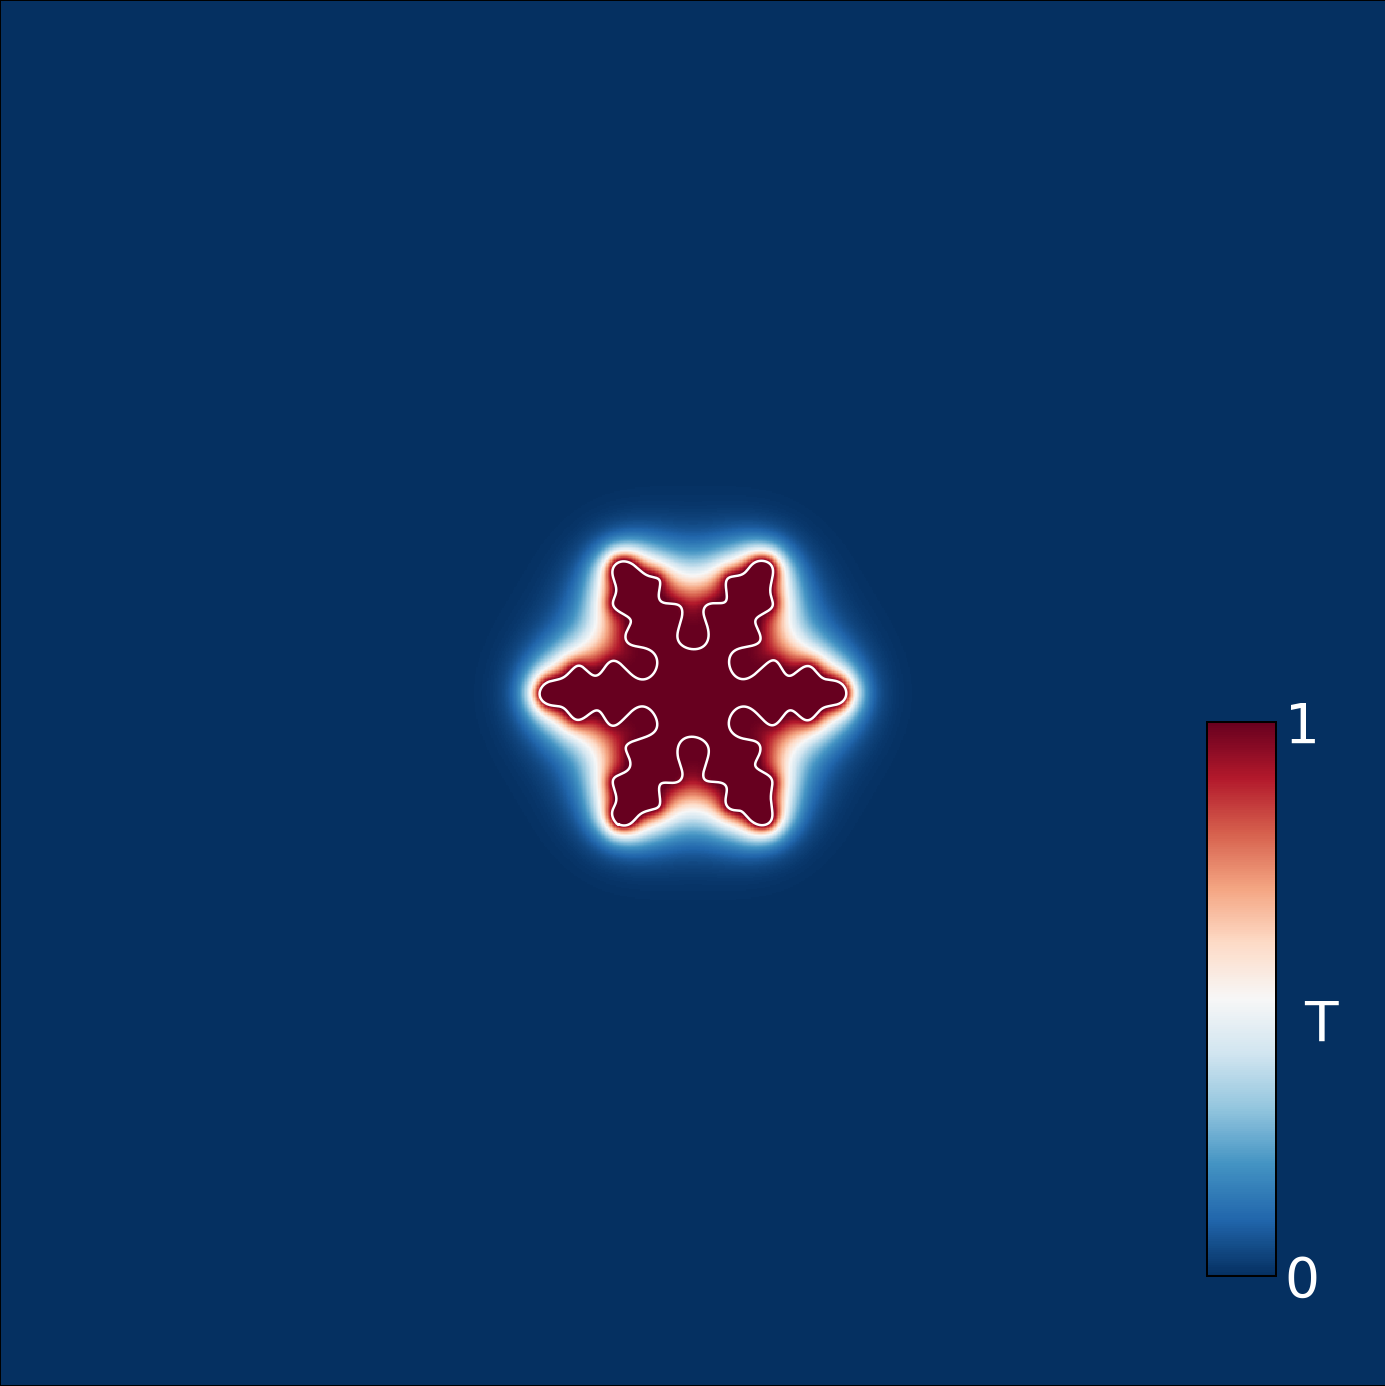
\includegraphics[width=\subfigwidth]{results/show_low_xi_U_5.png}} &
\raisebox{-0.5\height}{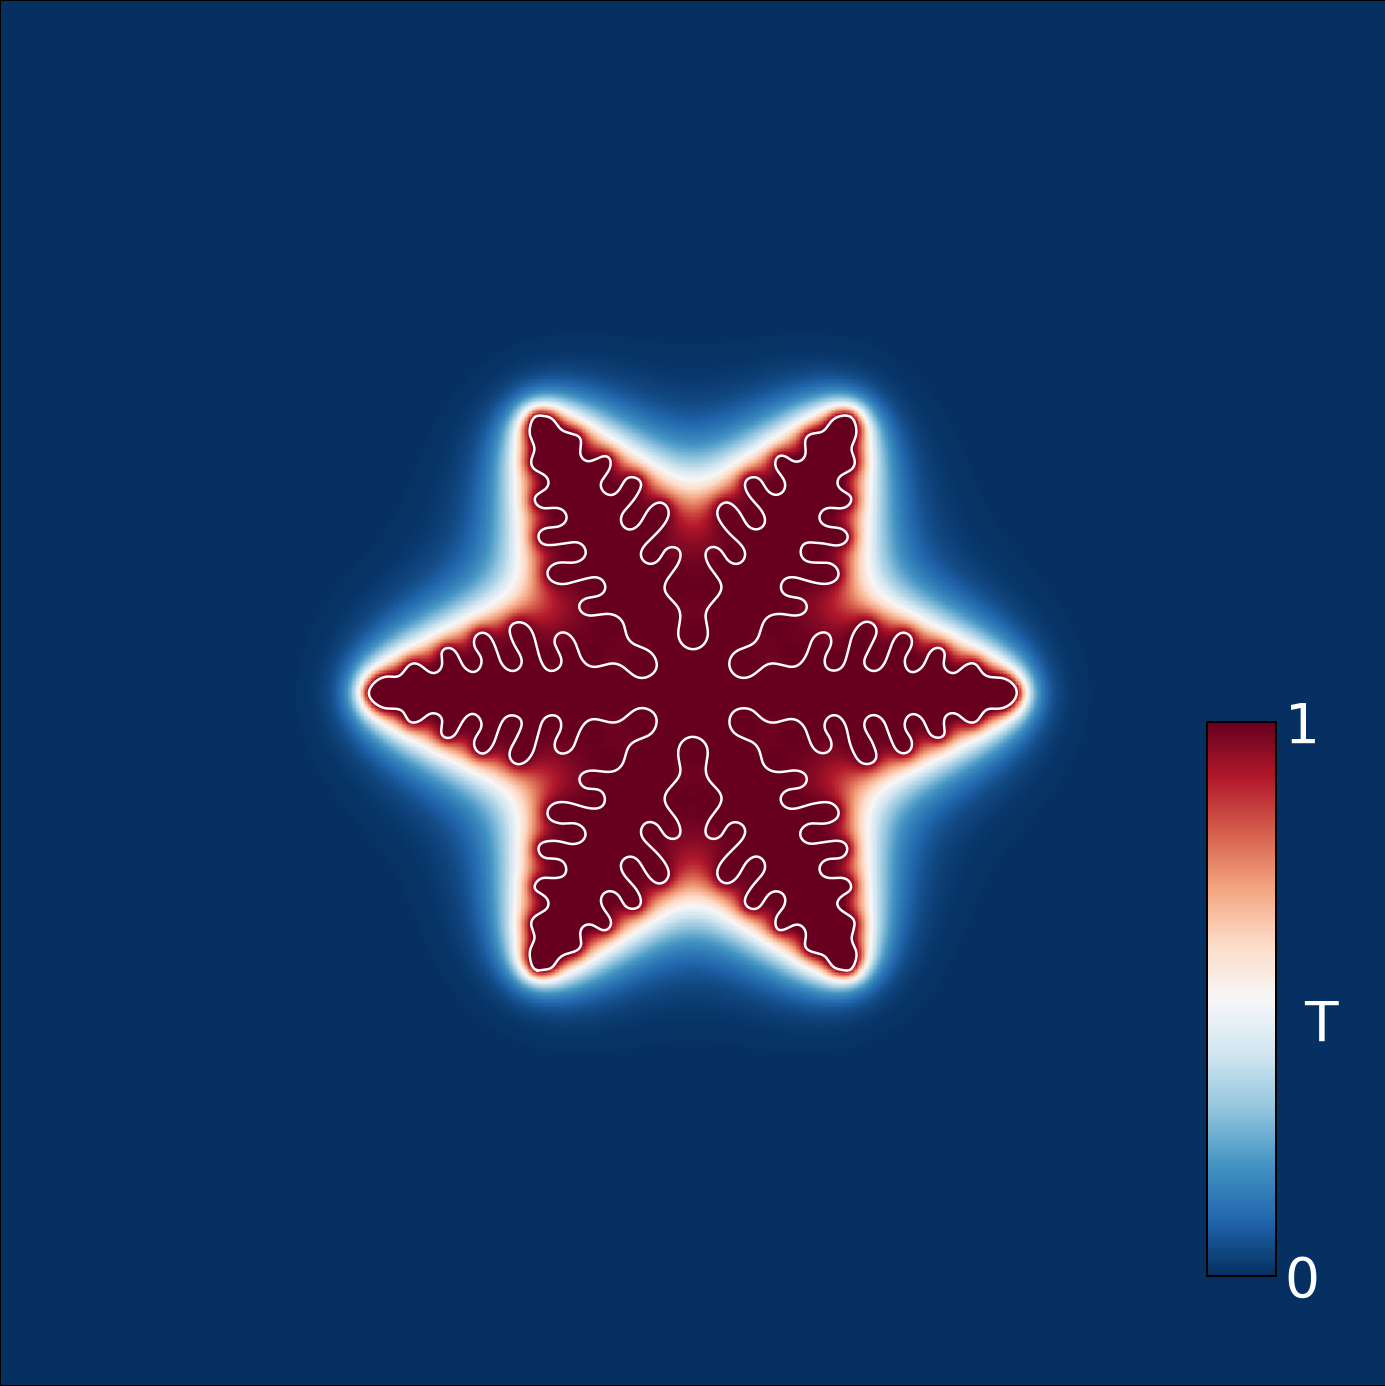
\includegraphics[width=\subfigwidth]{results/show_low_xi_U_13.png}} &
\raisebox{-0.5\height}{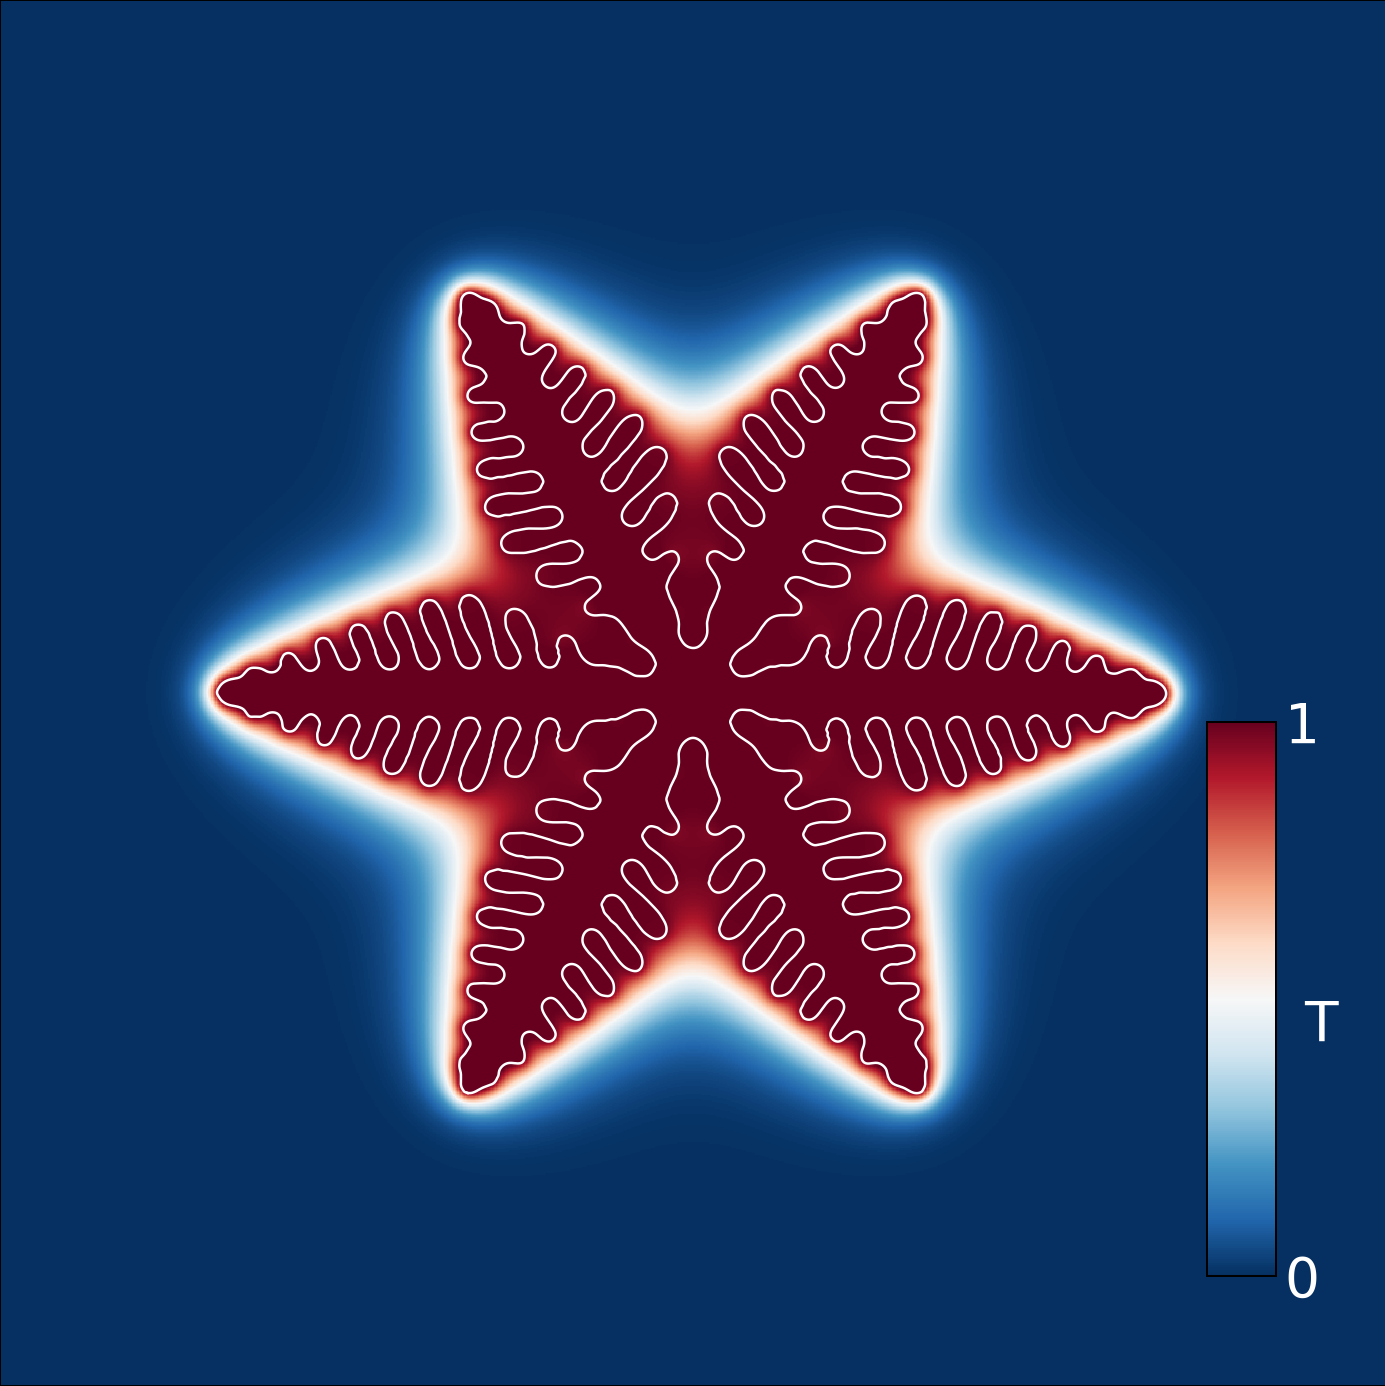
\includegraphics[width=\subfigwidth]{results/show_low_xi_U_20.png}} \\
$t = 0.01$ & 
$t = 0.0275$ & 
$t = 0.04$ 

\end{tabular}
    \caption{
        Evolution of the temperature field and the phase interface $\Gamma$ (in white) over the time interval $\Timeint = [0, 0.04]$ using the S-I scheme. Simulation setup given in Section \ref{sec:simulation setup} was used. The simulation running on hardware given in Section \ref{sec:algorithm benchmarks} run for 354 seconds, with average time of 44 milliseconds per iteration. The conjugate gradient method used in the S-I scheme performed on 4 iterations to converge for the phase field and 6 iterations to converge for the temperature field. Note that the performance characteristics of the S-I scheme are hard to generalize as the convergence and thus runtime is partly determined by the choice of model parameters.
    }
    \label{fig:def params results}
\end{figure}
\FloatBarrier

\setlength{\subfigwidth}{0.31\textwidth}
\FloatBarrier
\begin{figure}[!ht]
    \centering
    \begin{tabular}{P{\subfigwidth}P{\subfigwidth}P{\subfigwidth}}
    
    \raisebox{-0.5\height}{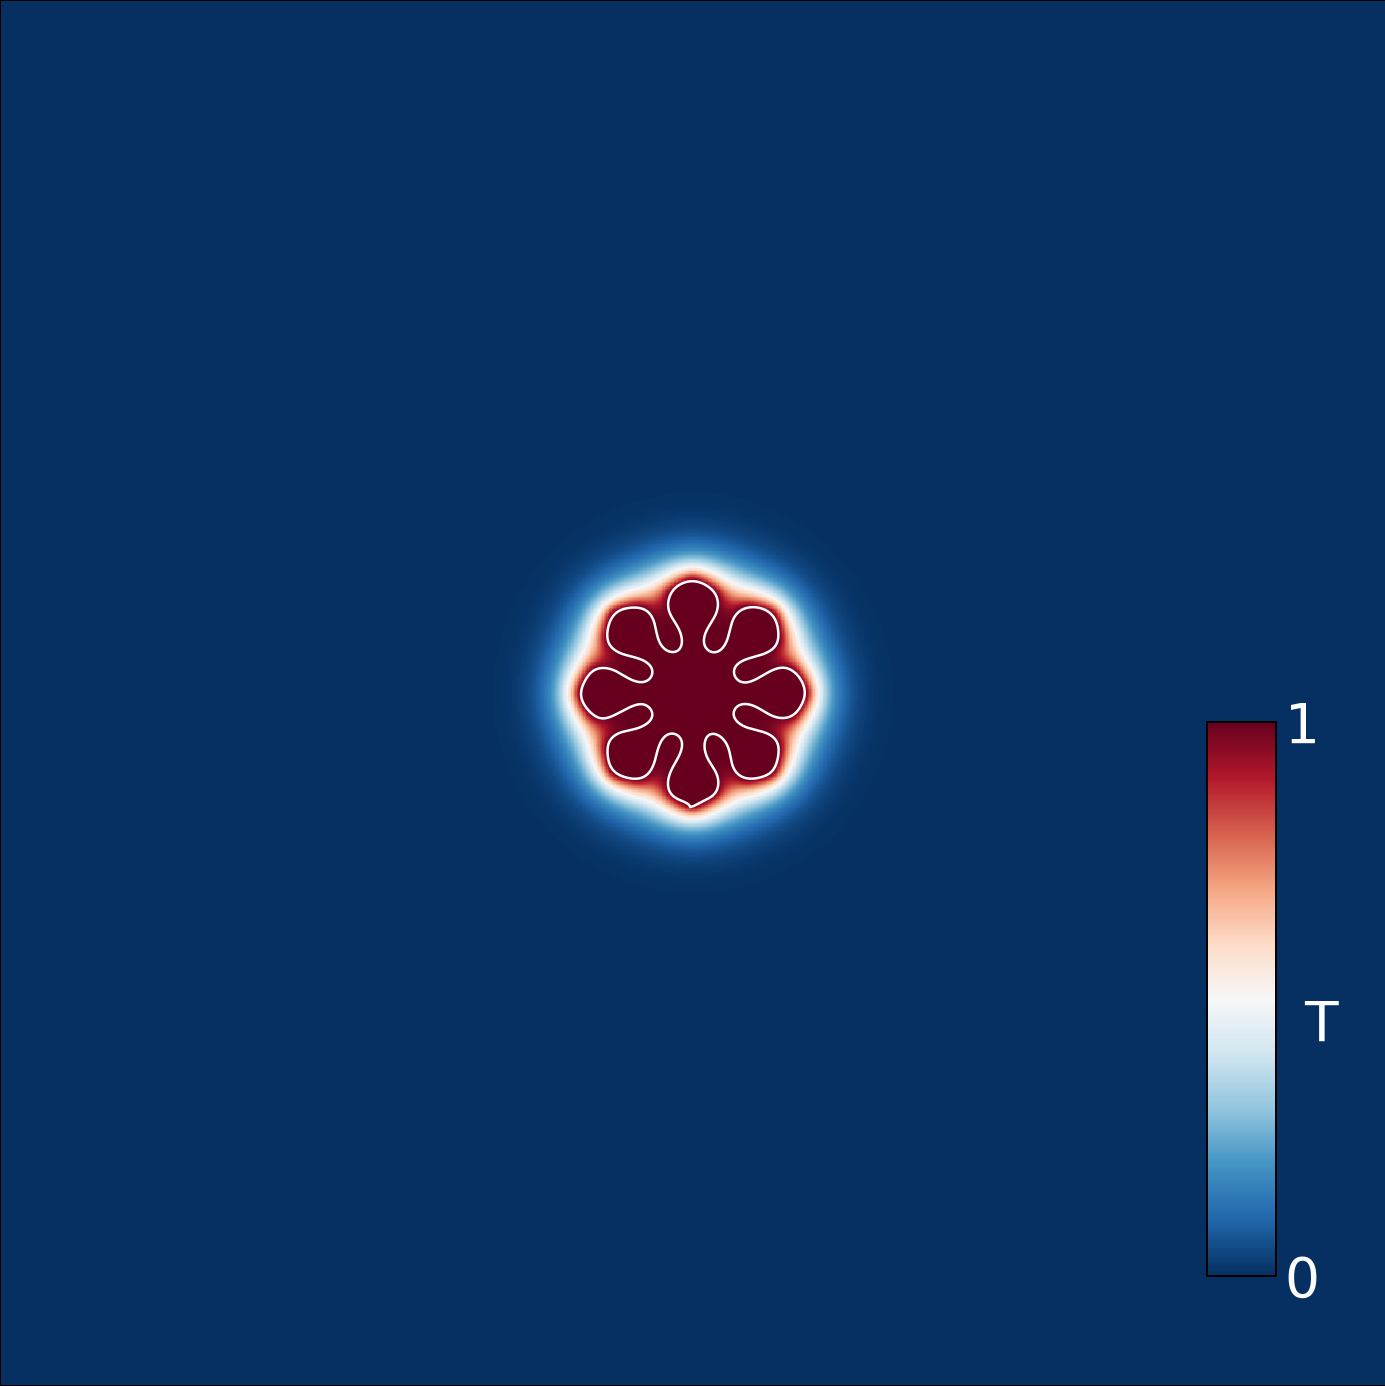
\includegraphics[width=\subfigwidth]{results/show_low_xi_anisofold_8_U_6.png}} &
    \raisebox{-0.5\height}{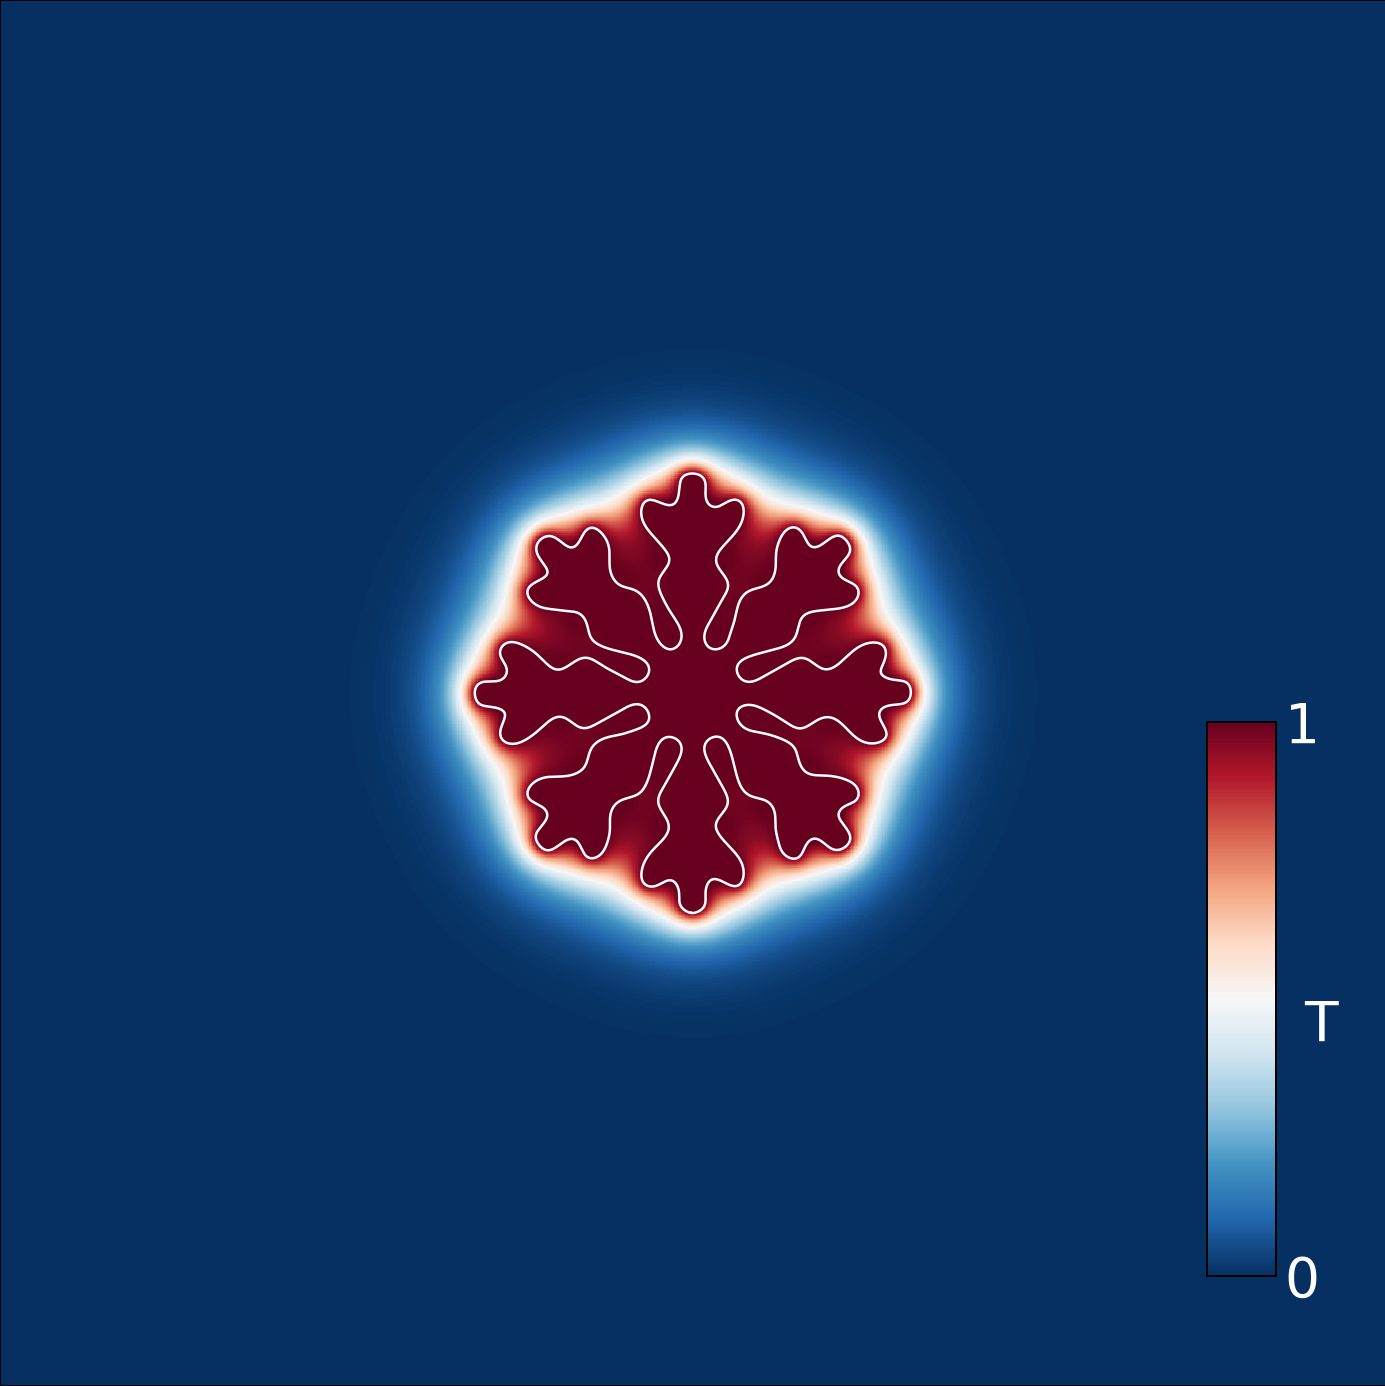
\includegraphics[width=\subfigwidth]{results/show_low_xi_anisofold_8_U_18.png}} &
    \raisebox{-0.5\height}{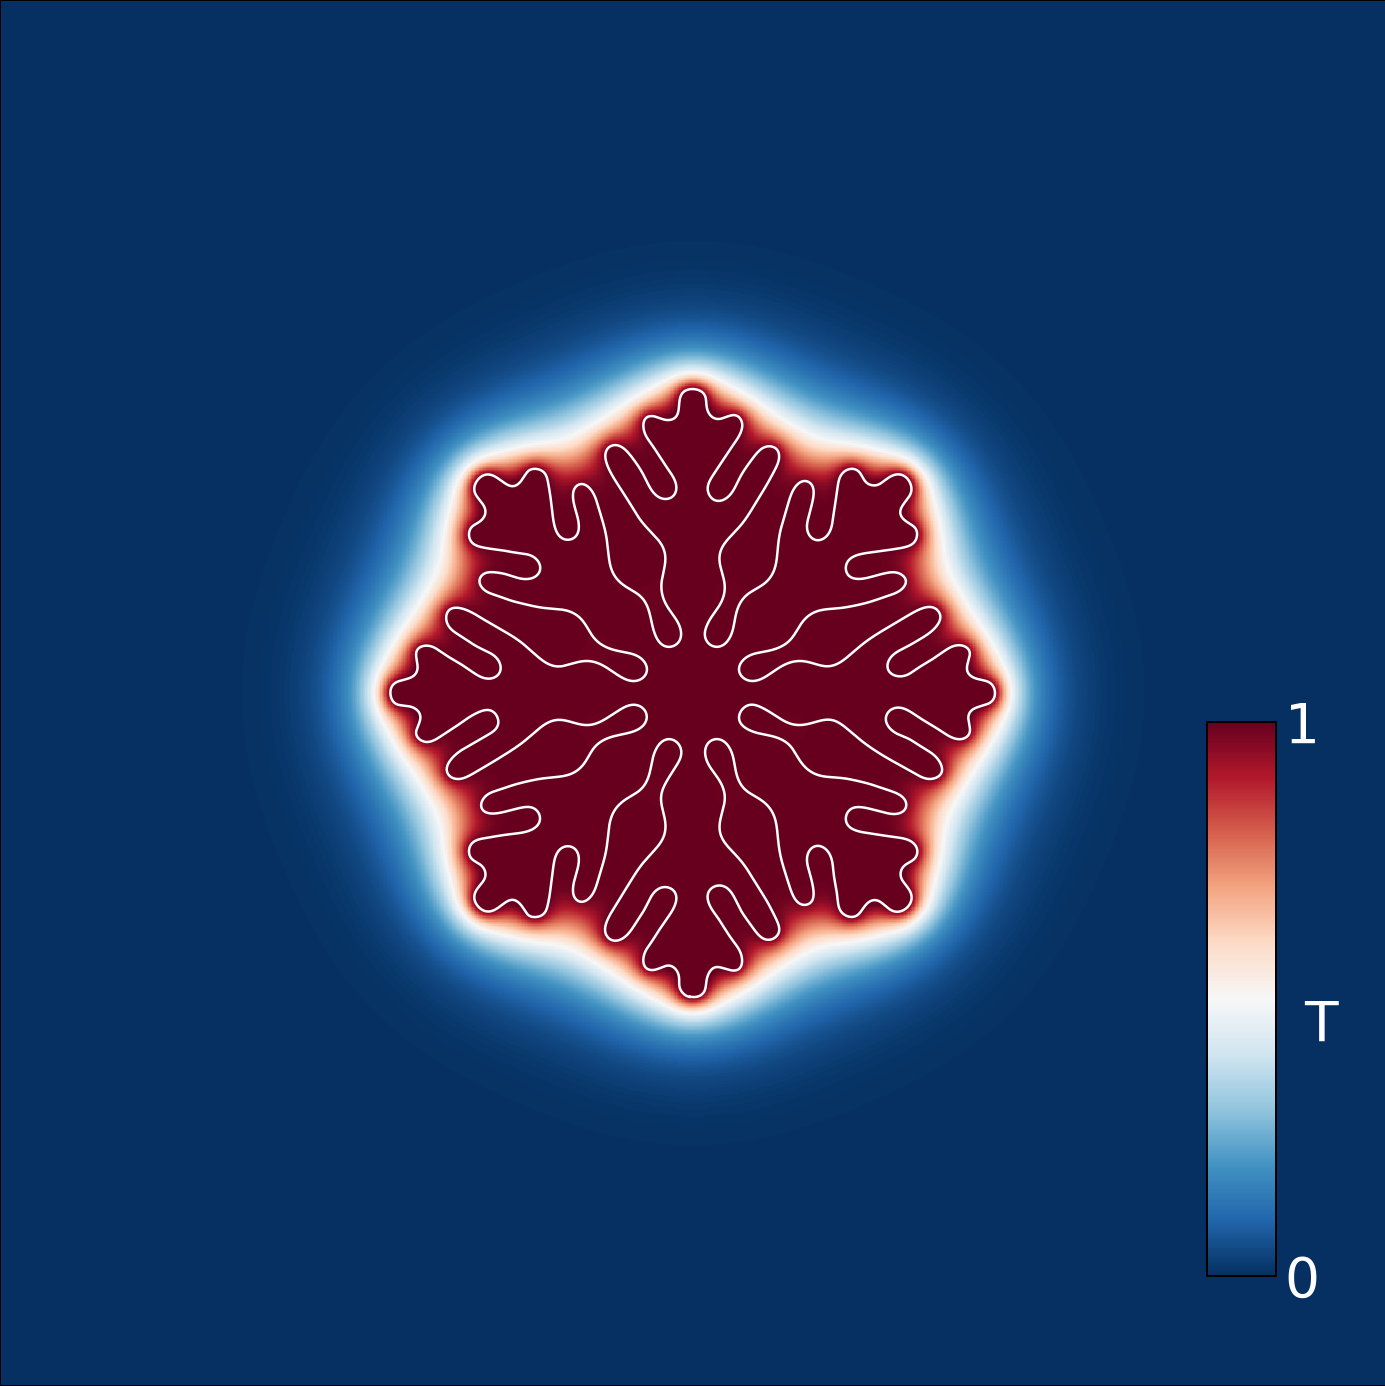
\includegraphics[width=\subfigwidth]{results/show_low_xi_anisofold_8_U_30.png}} \\
    $t = 0.01$ & 
    $t = 0.032$ & 
    $t = 0.06$ 
    
    \end{tabular}
    \caption{Evolution of the temperature field and the phase interface $\Gamma$ (in white) over the time interval $\Timeint = [0, 0.06]$  using the S-I scheme. Simulation setup given in Section \ref{sec:simulation setup} was used. Anisotropy has been changed to 8-fold.
    }
    \label{fig:s-i coarsening}
\end{figure}
\FloatBarrier


\setlength{\subfigwidth}{0.29\textwidth}

\FloatBarrier
\begin{figure}[!ht]
    \centering
    \begin{tabular}{r P{\subfigwidth}P{\subfigwidth}P{\subfigwidth}}
    
    \rotatebox{90}{} & 
    $\xi = 0.0025$ &
    $\xi = 0.0043$ &
    $\xi = 0.0065$ \\
    
    \rotatebox[origin=c]{90}{$t = 0.01$} & 
    \raisebox{-0.5\height}{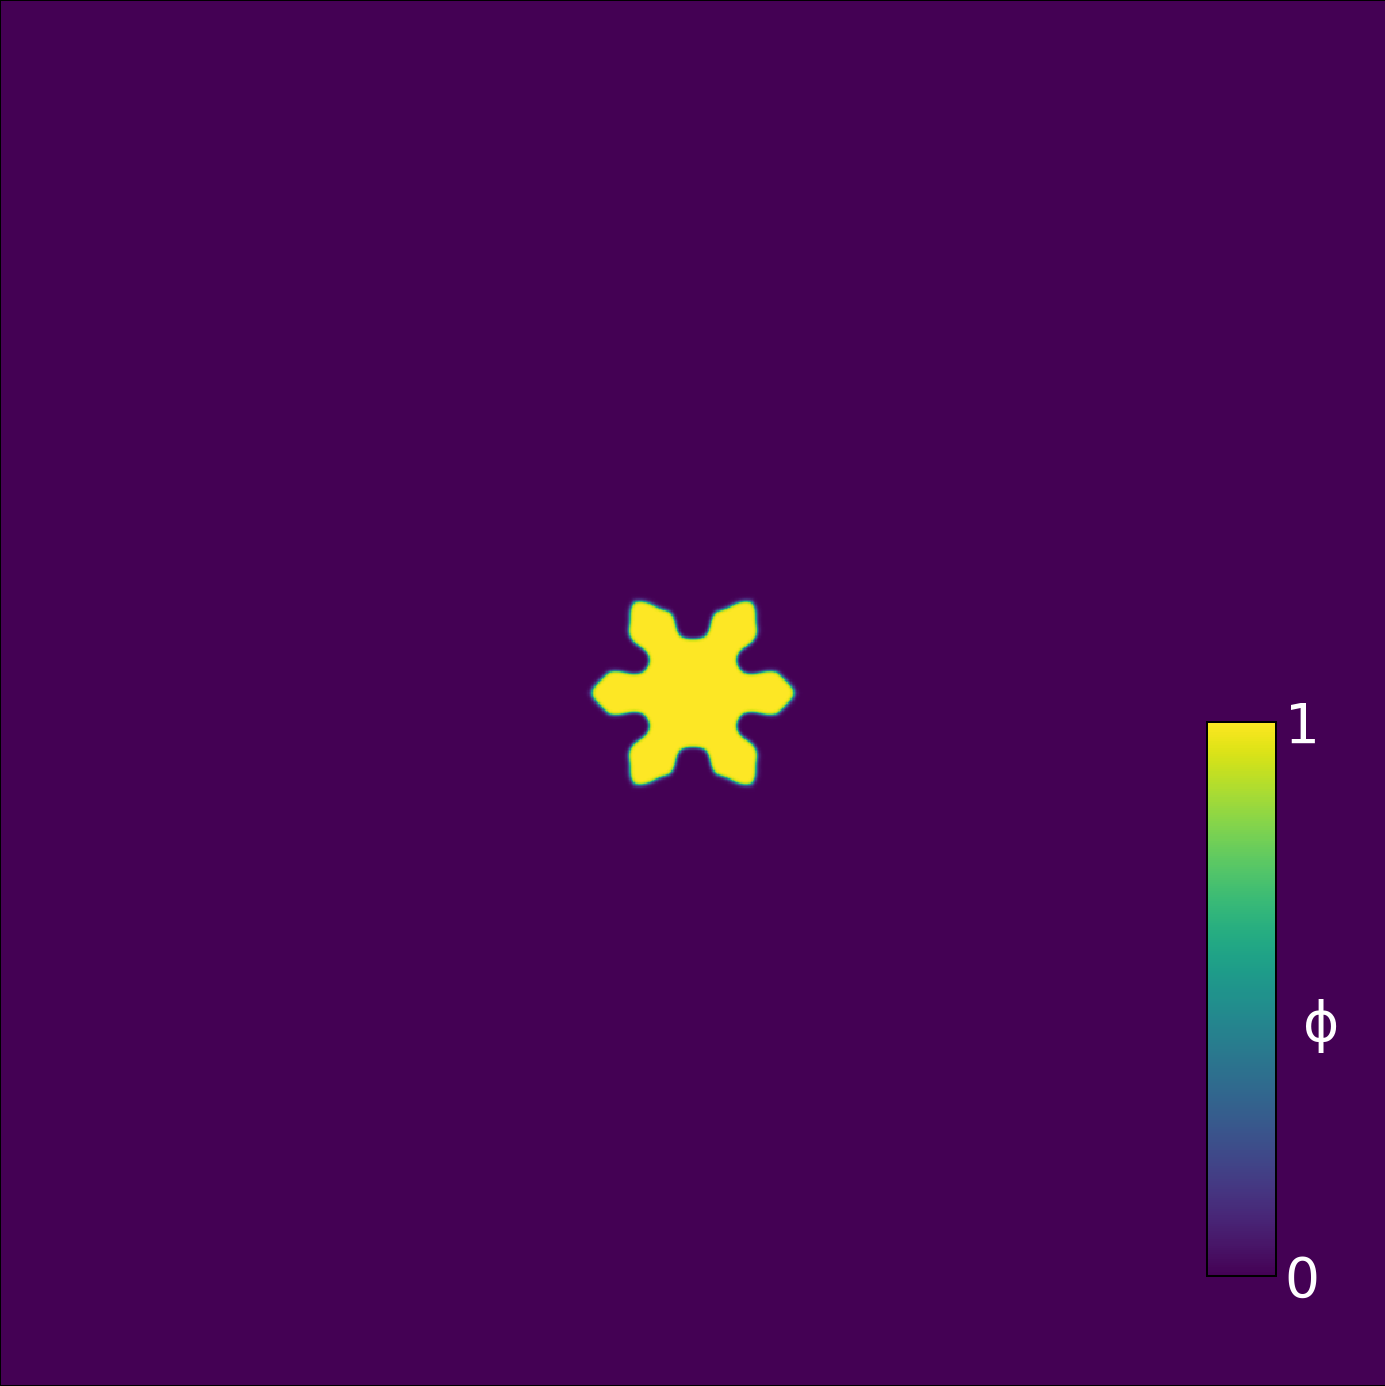
\includegraphics[width=\subfigwidth]{results/show_tiny_xi_F_5.png}} &
    \raisebox{-0.5\height}{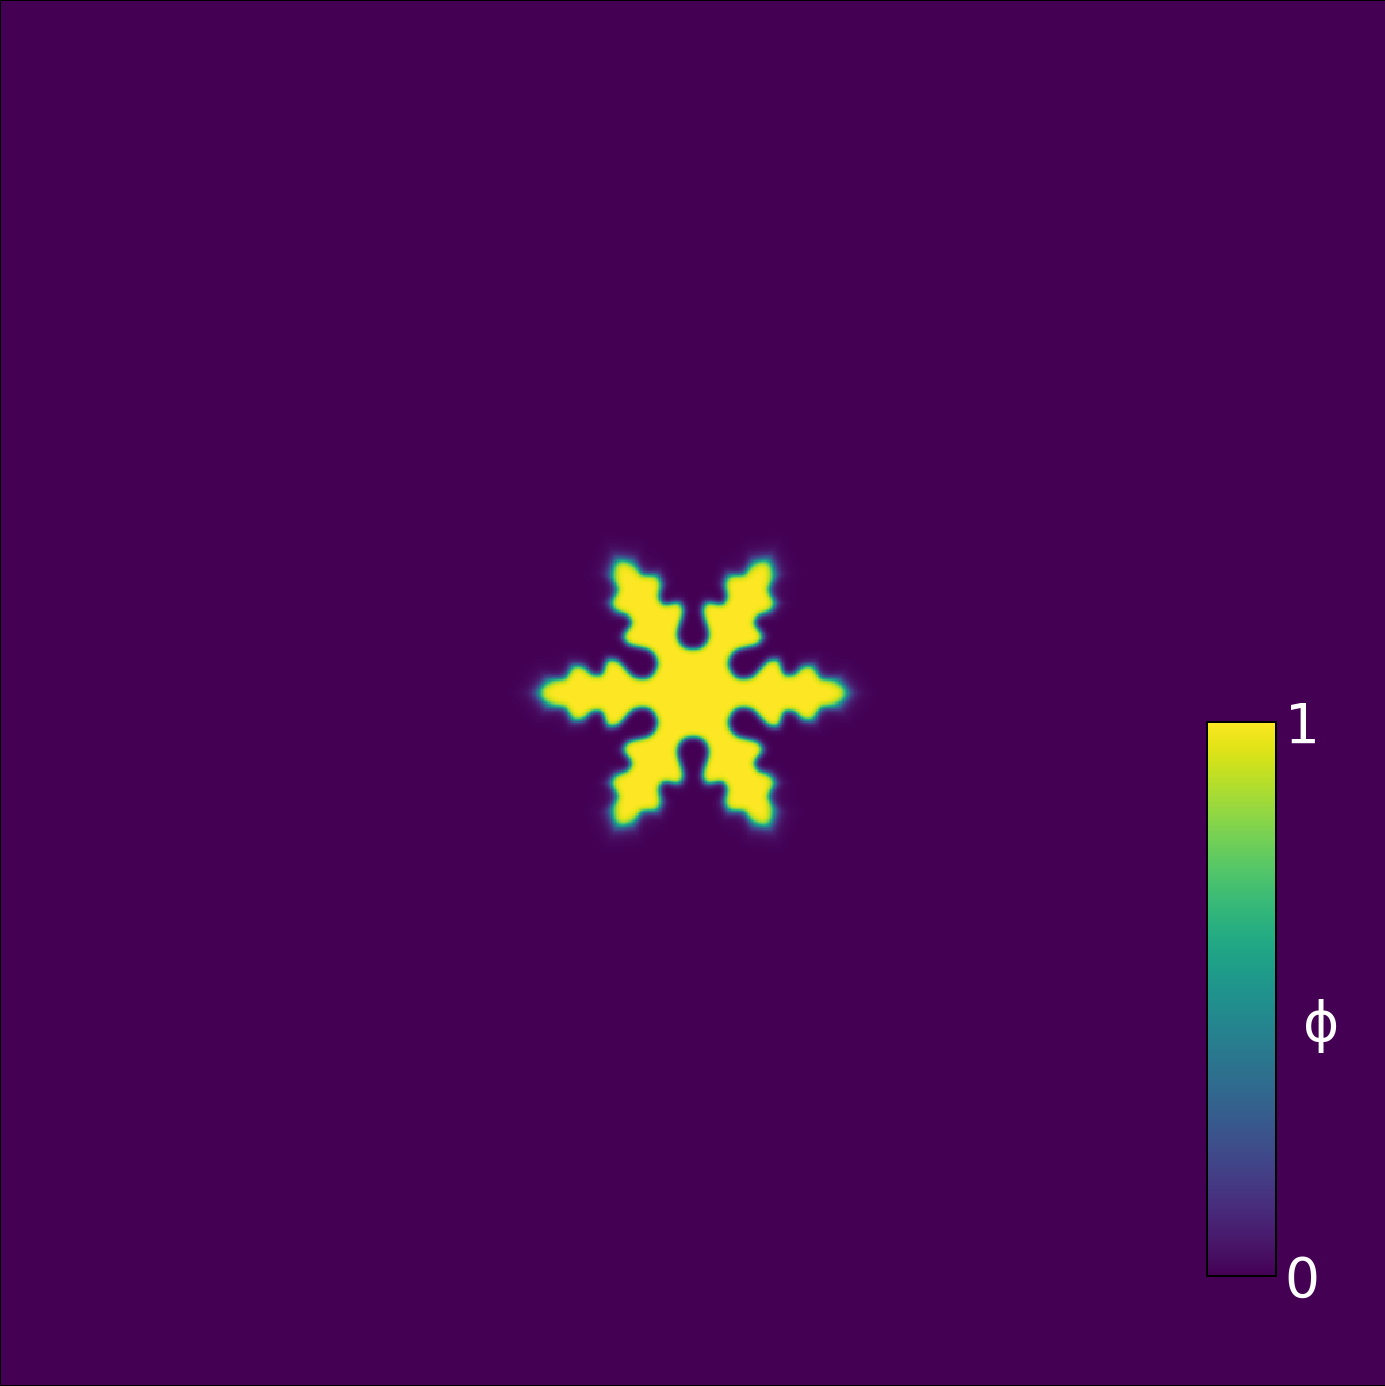
\includegraphics[width=\subfigwidth]{results/show_low_xi_F_5.png}} &
    \raisebox{-0.5\height}{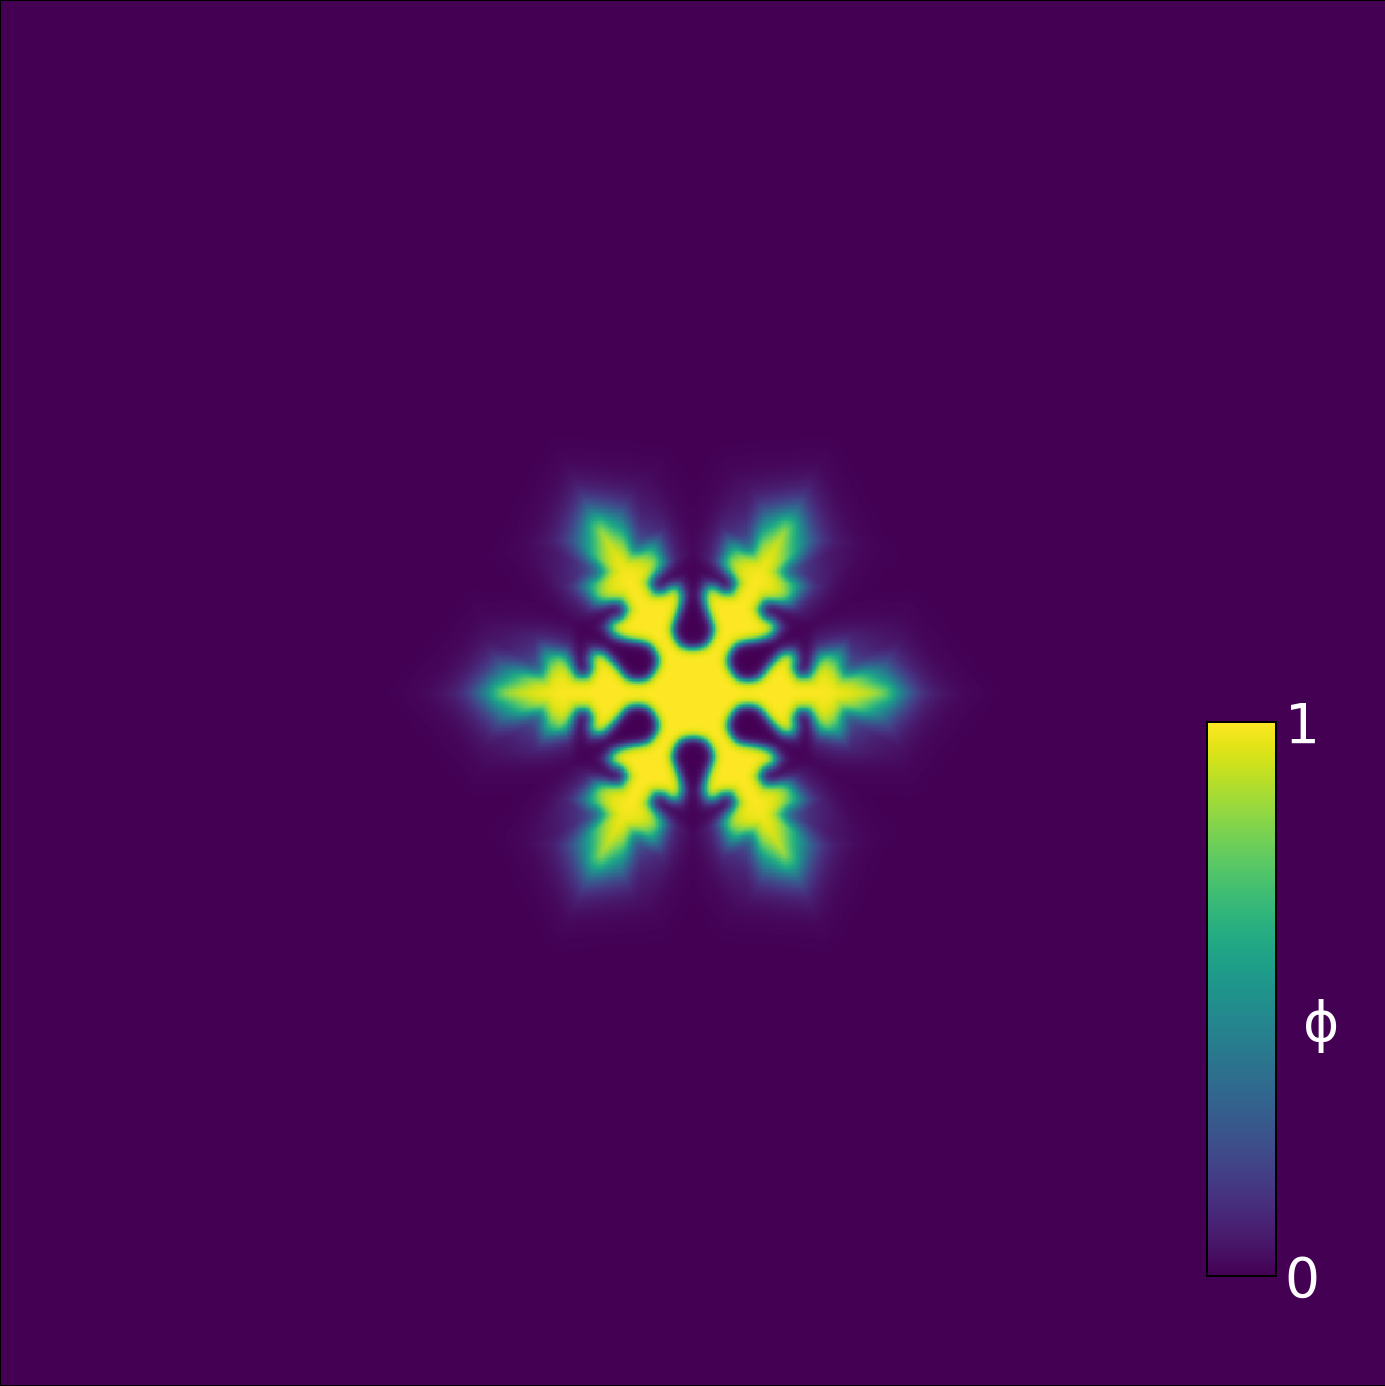
\includegraphics[width=\subfigwidth]{results/show_medium_xi_F_5.png}} \\
    \\
    \rotatebox[origin=c]{90}{$t = 0.0275$} & 
    \raisebox{-0.5\height}{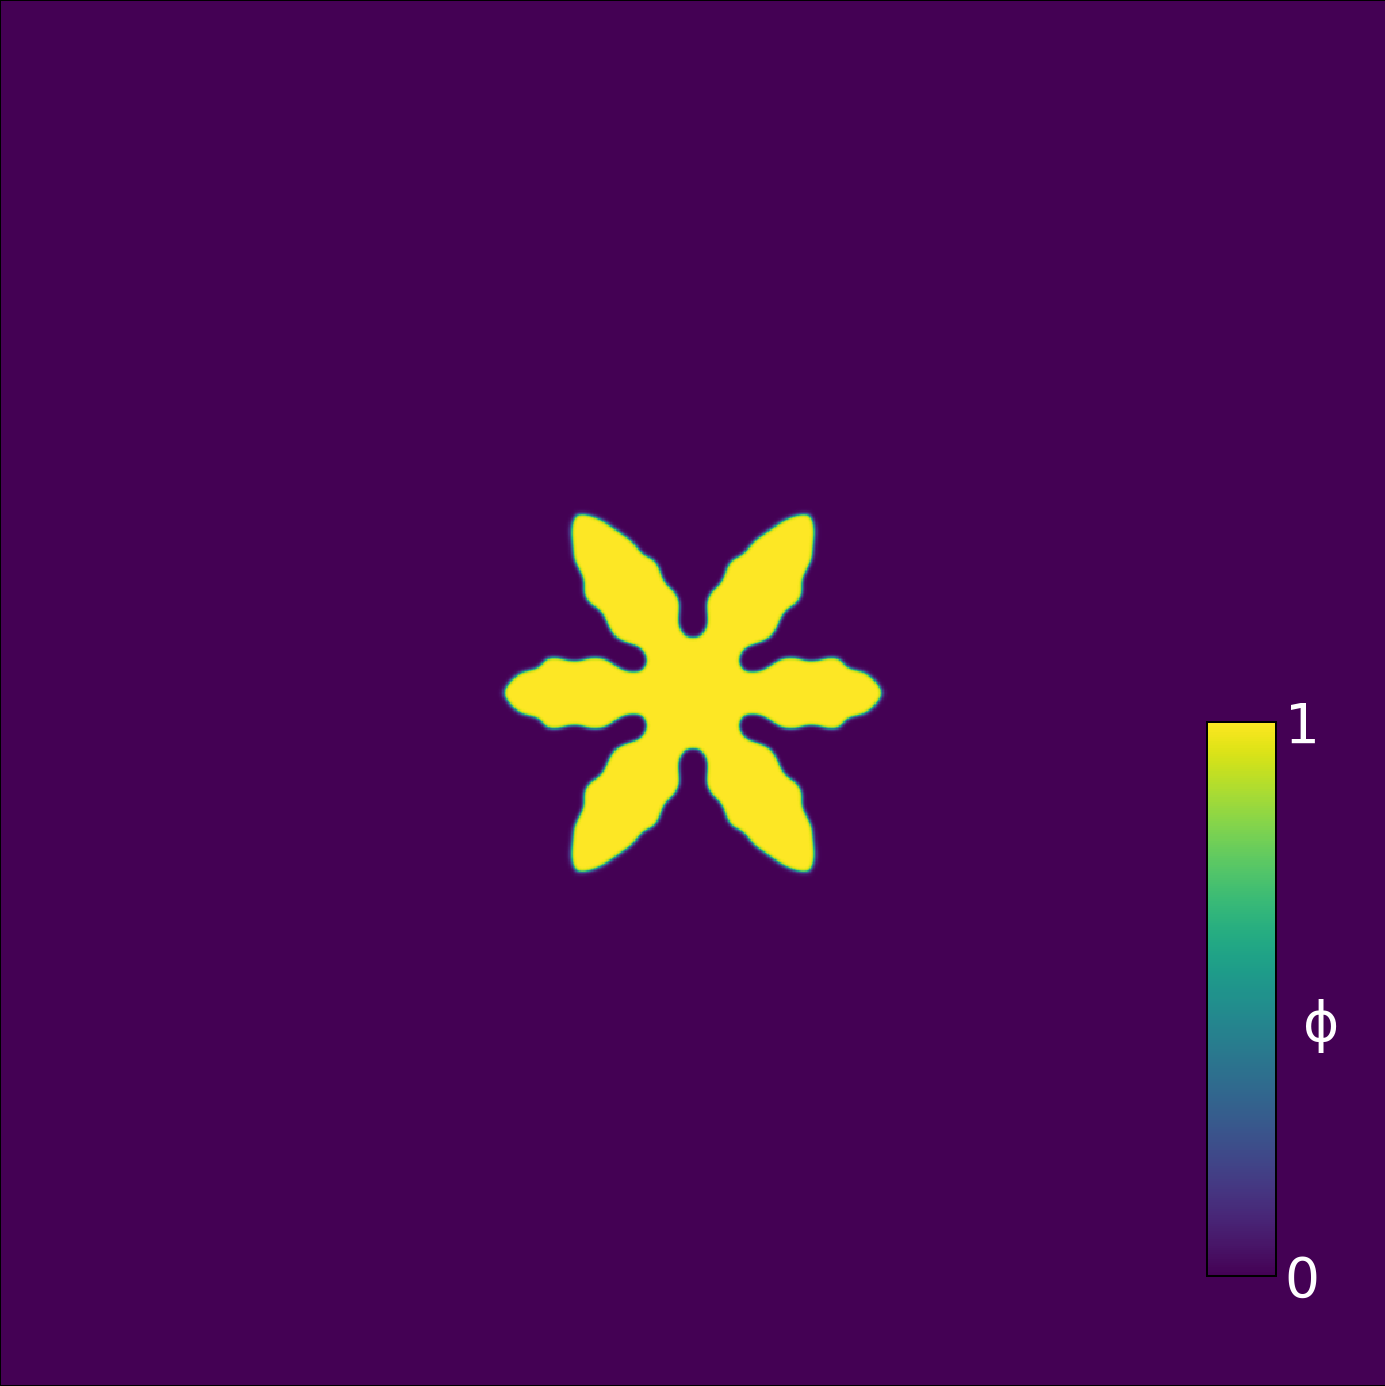
\includegraphics[width=\subfigwidth]{results/show_tiny_xi_F_13.png}} &
    \raisebox{-0.5\height}{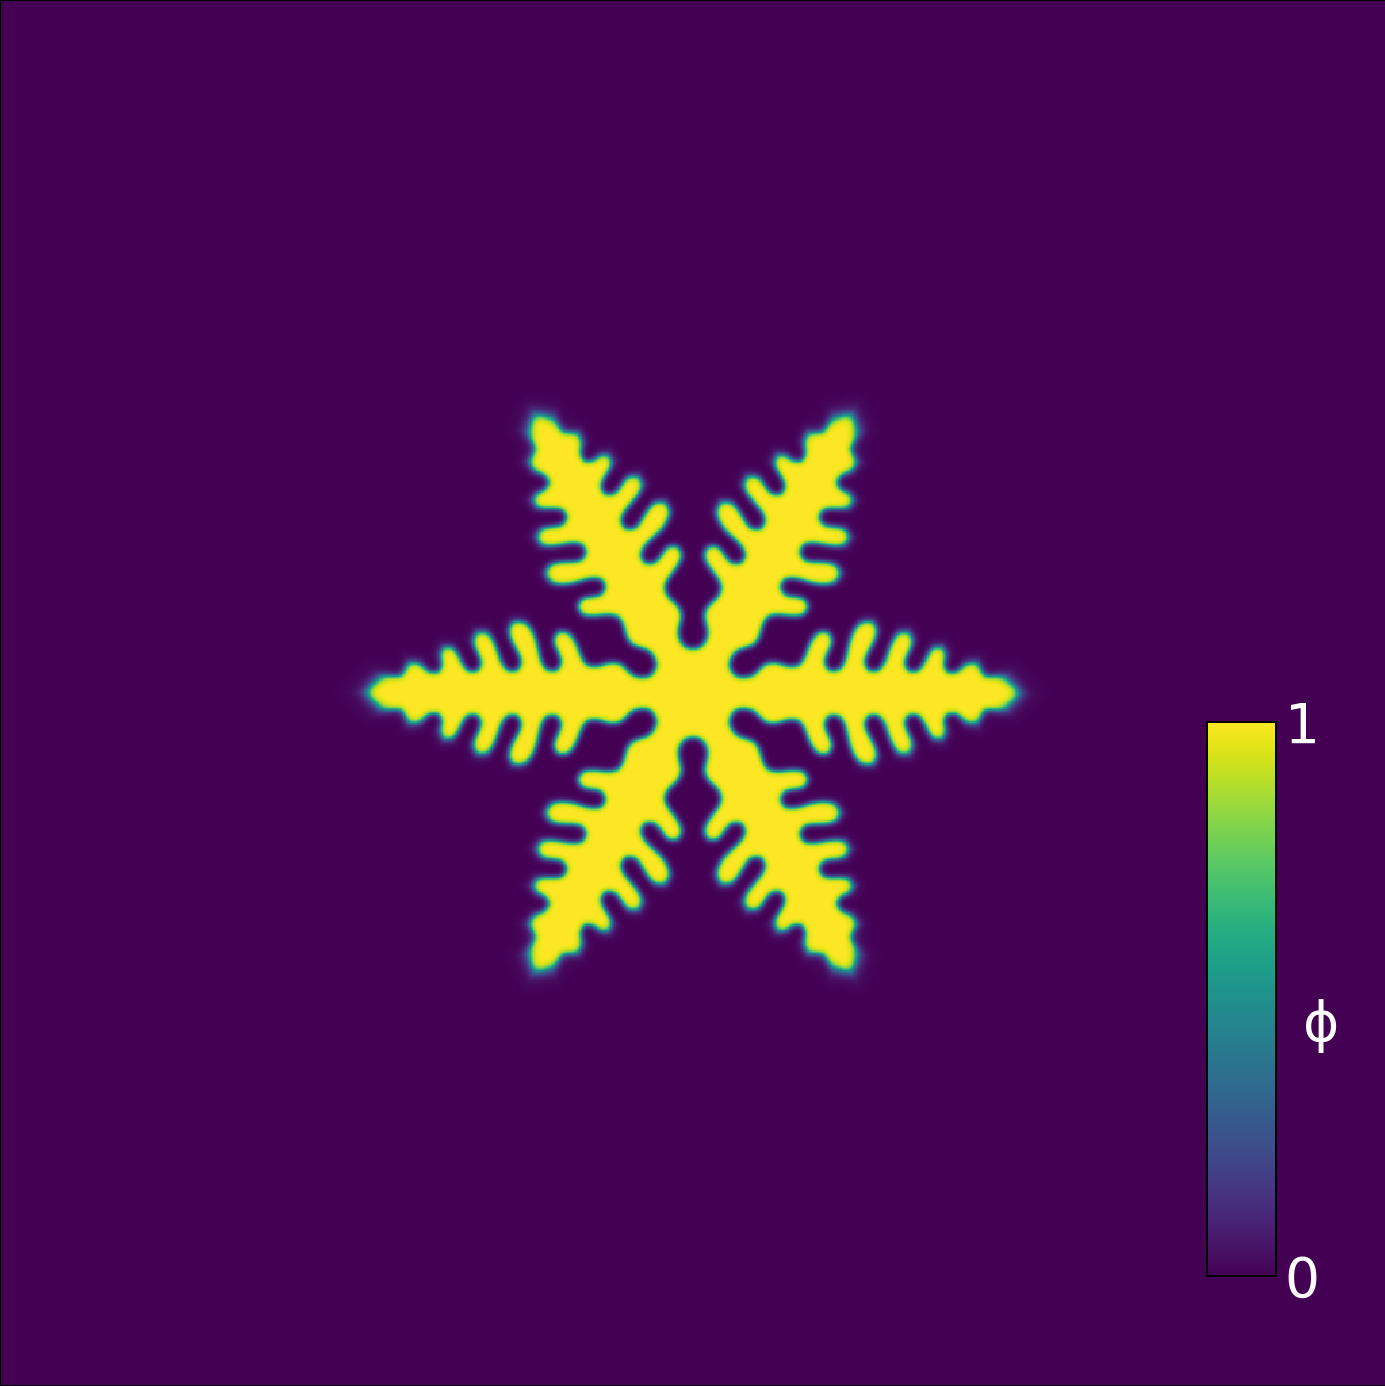
\includegraphics[width=\subfigwidth]{results/show_low_xi_F_13.png}} &
    \raisebox{-0.5\height}{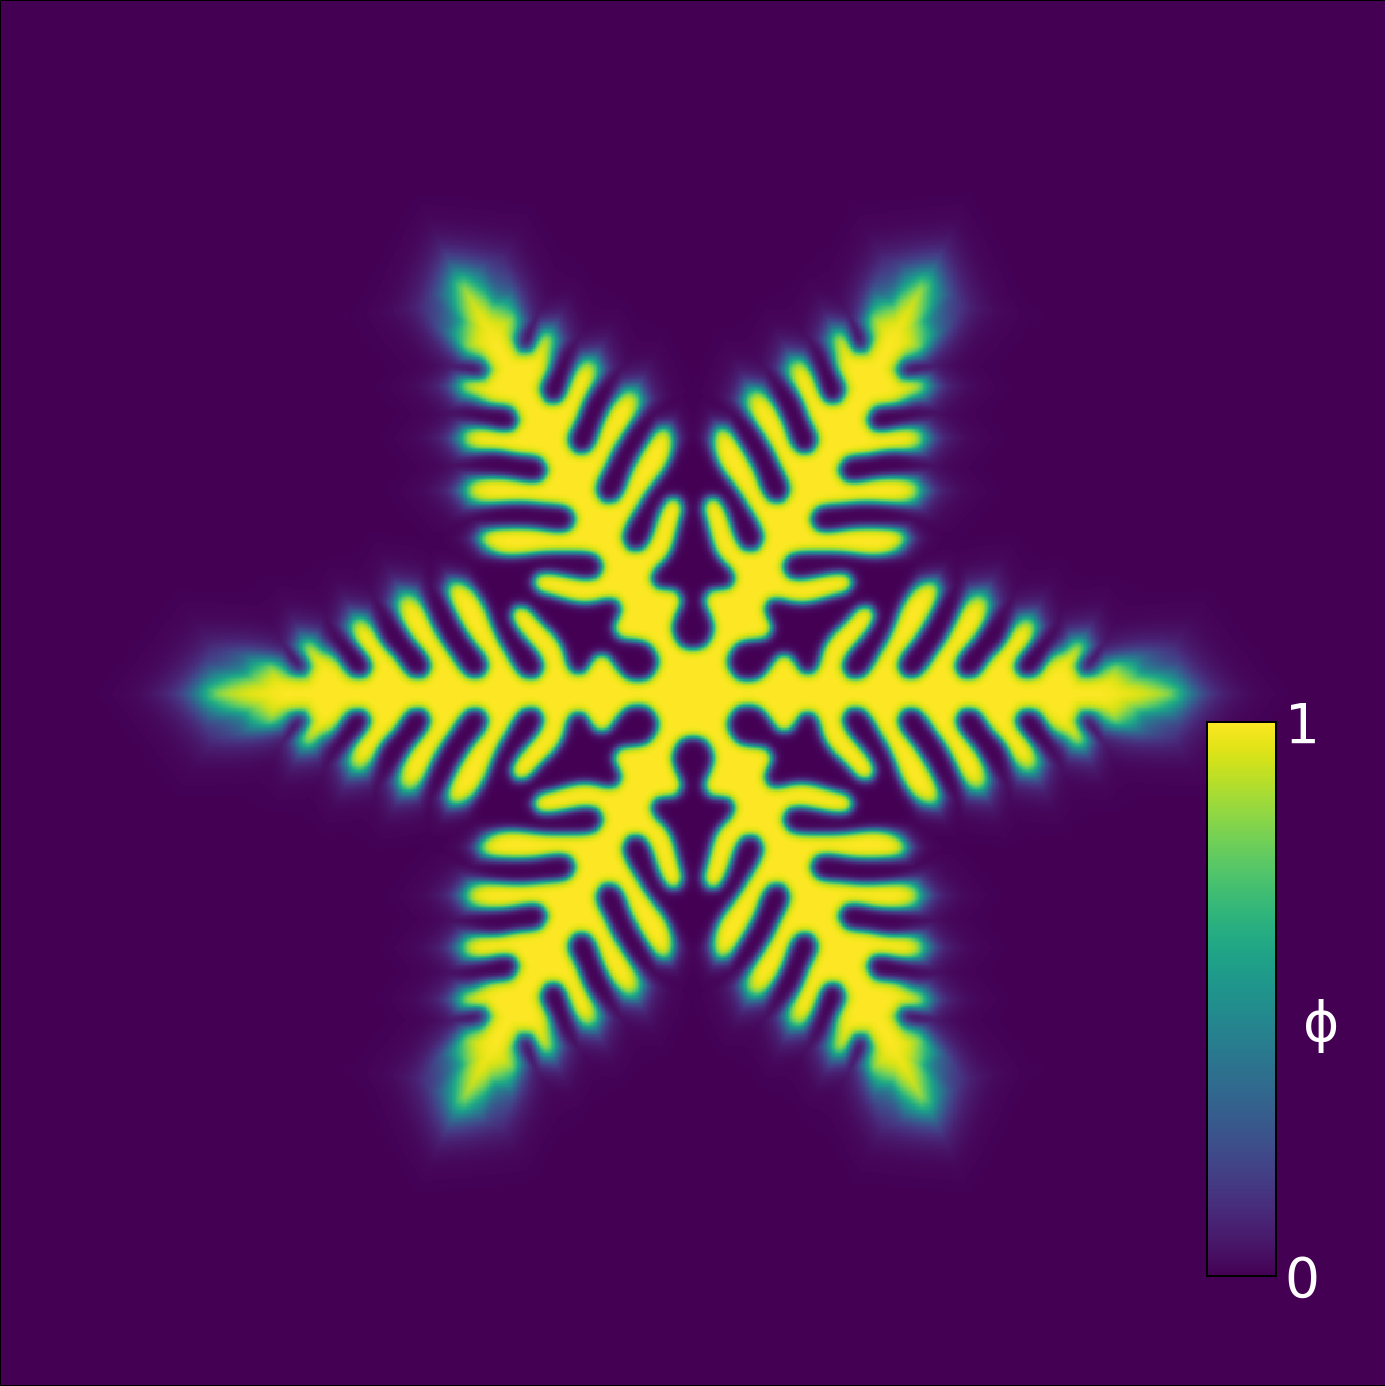
\includegraphics[width=\subfigwidth]{results/show_medium_xi_F_13.png}} \\
    \\
    \rotatebox[origin=c]{90}{$t = 0.04$} & 
    \raisebox{-0.5\height}{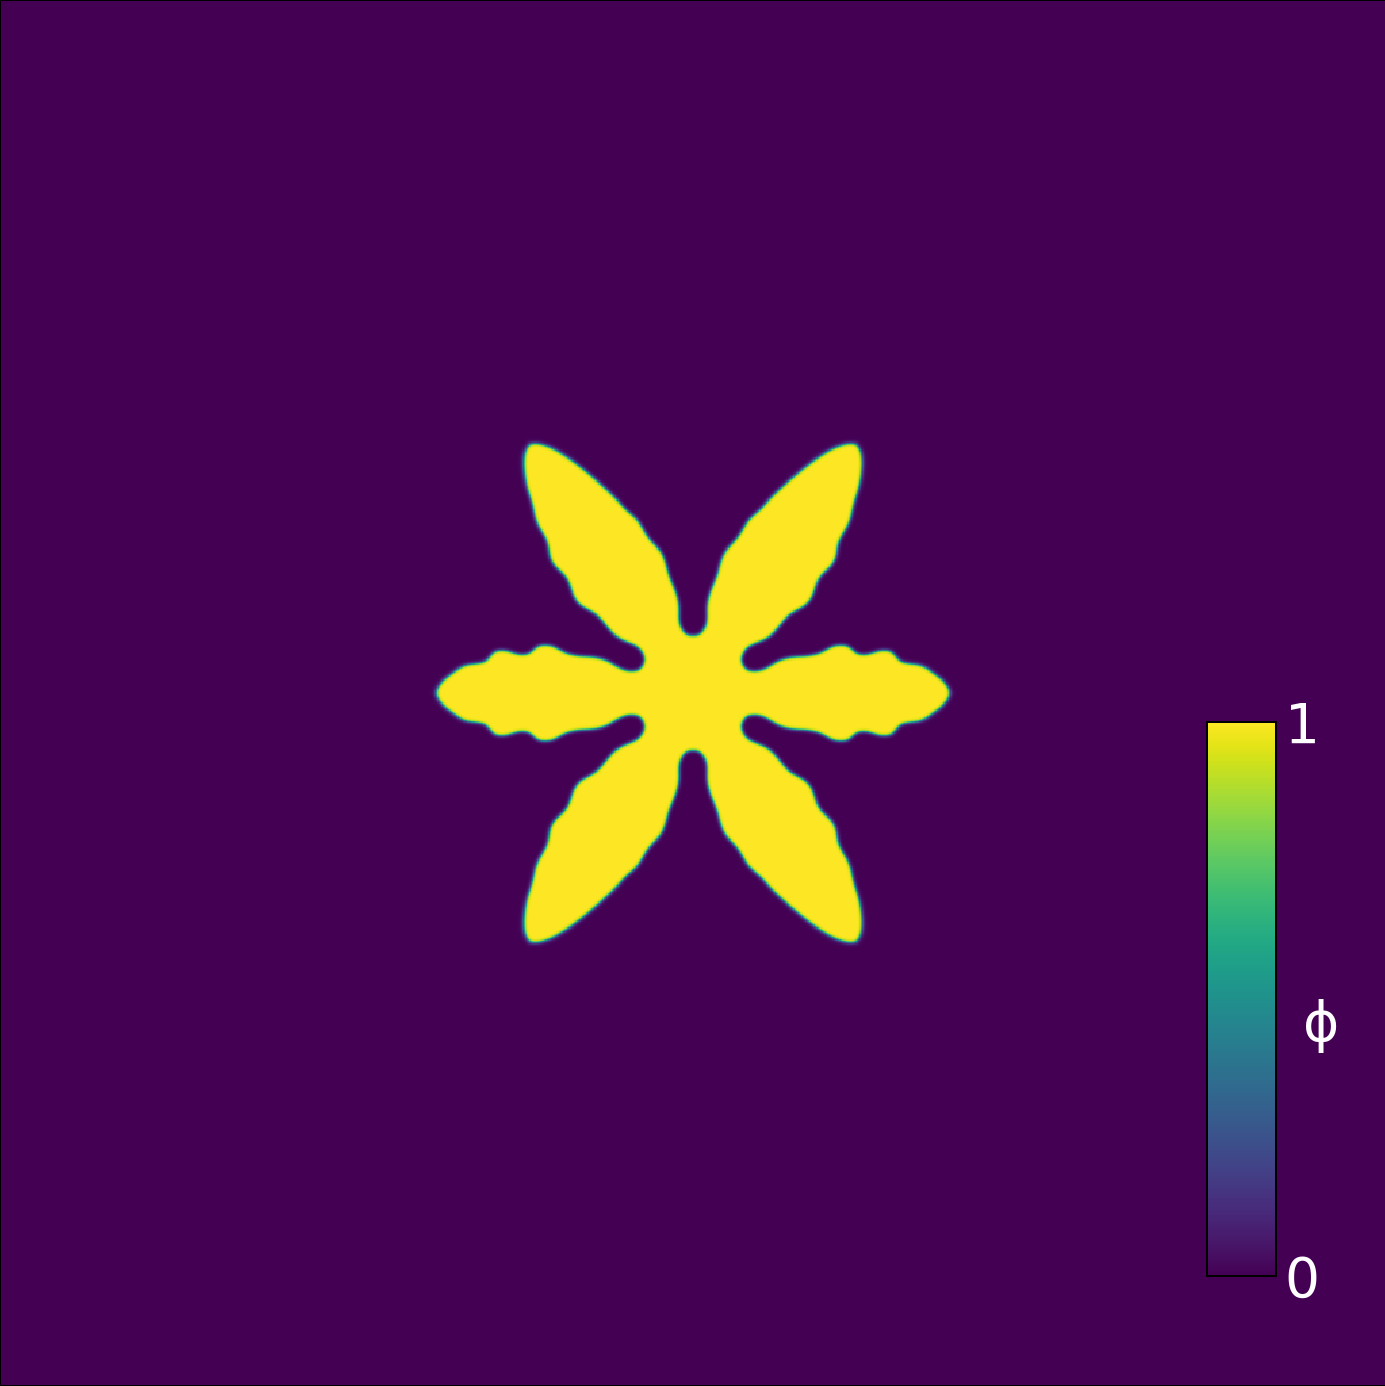
\includegraphics[width=\subfigwidth]{results/show_tiny_xi_F_20.png}} &
    \raisebox{-0.5\height}{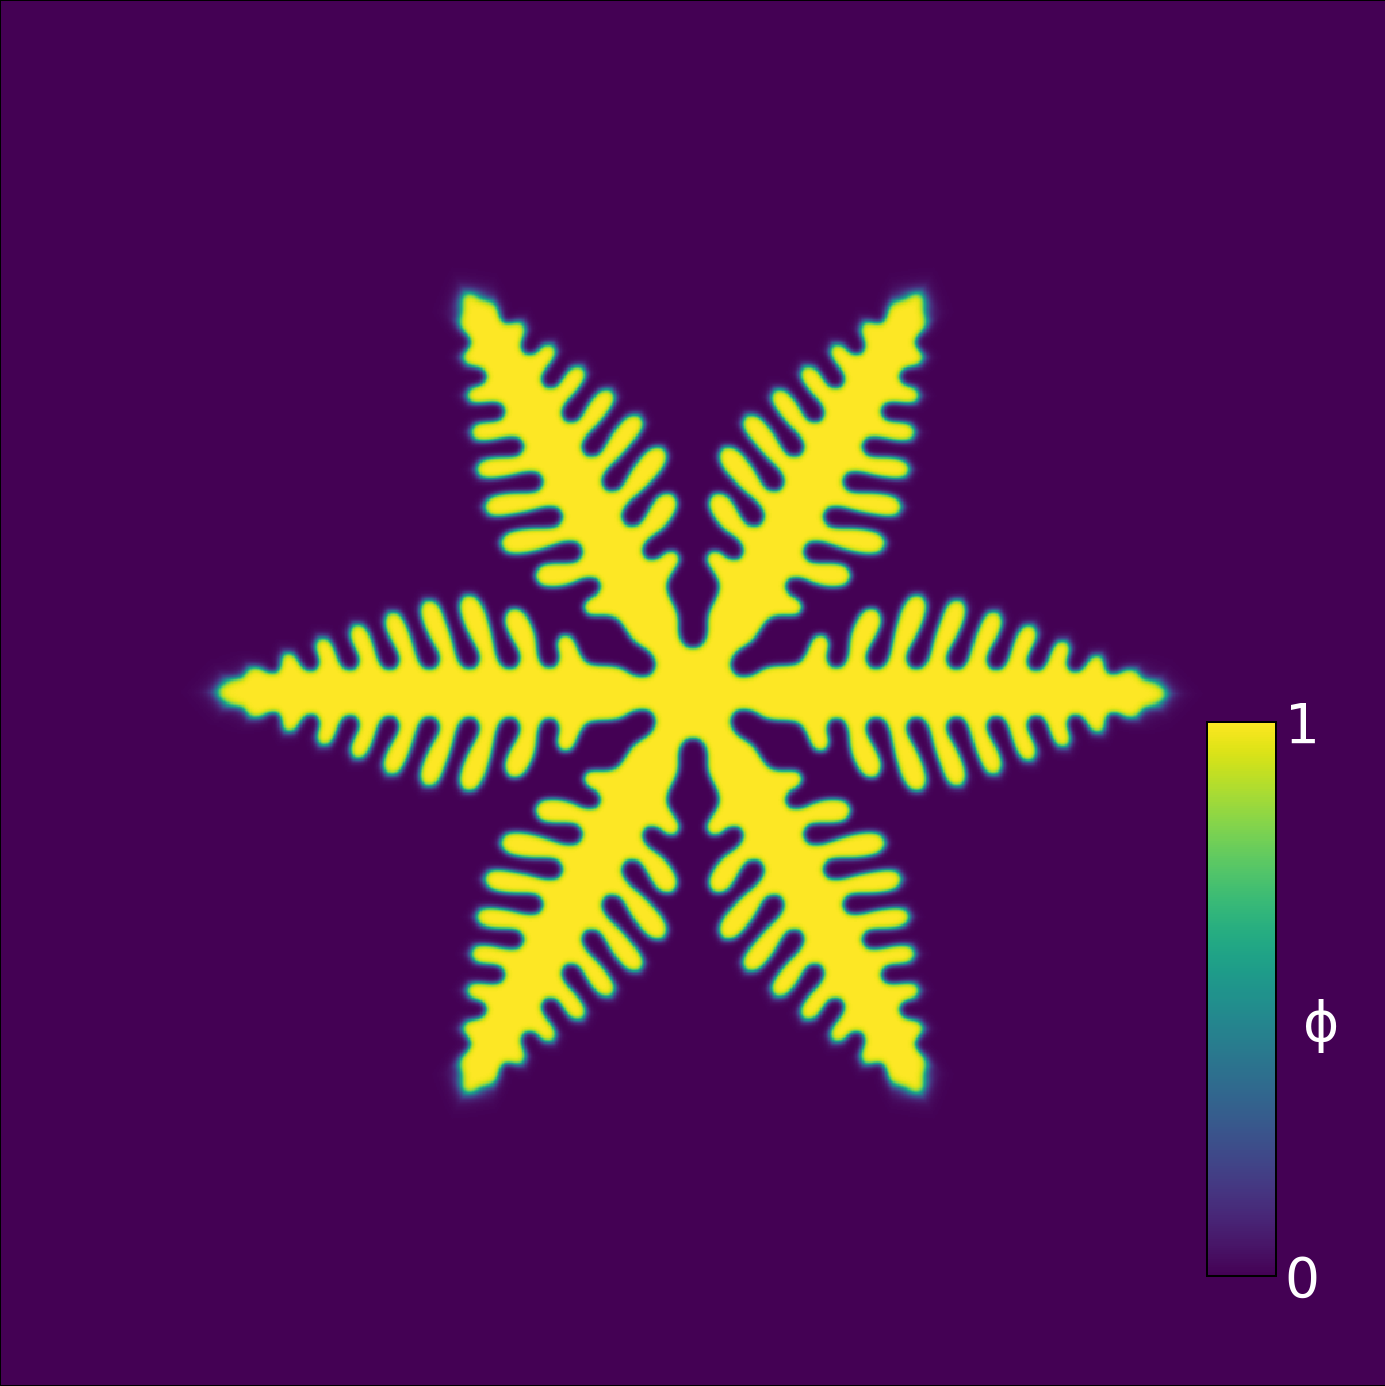
\includegraphics[width=\subfigwidth]{results/show_low_xi_F_20.png}} &
    \raisebox{-0.5\height}{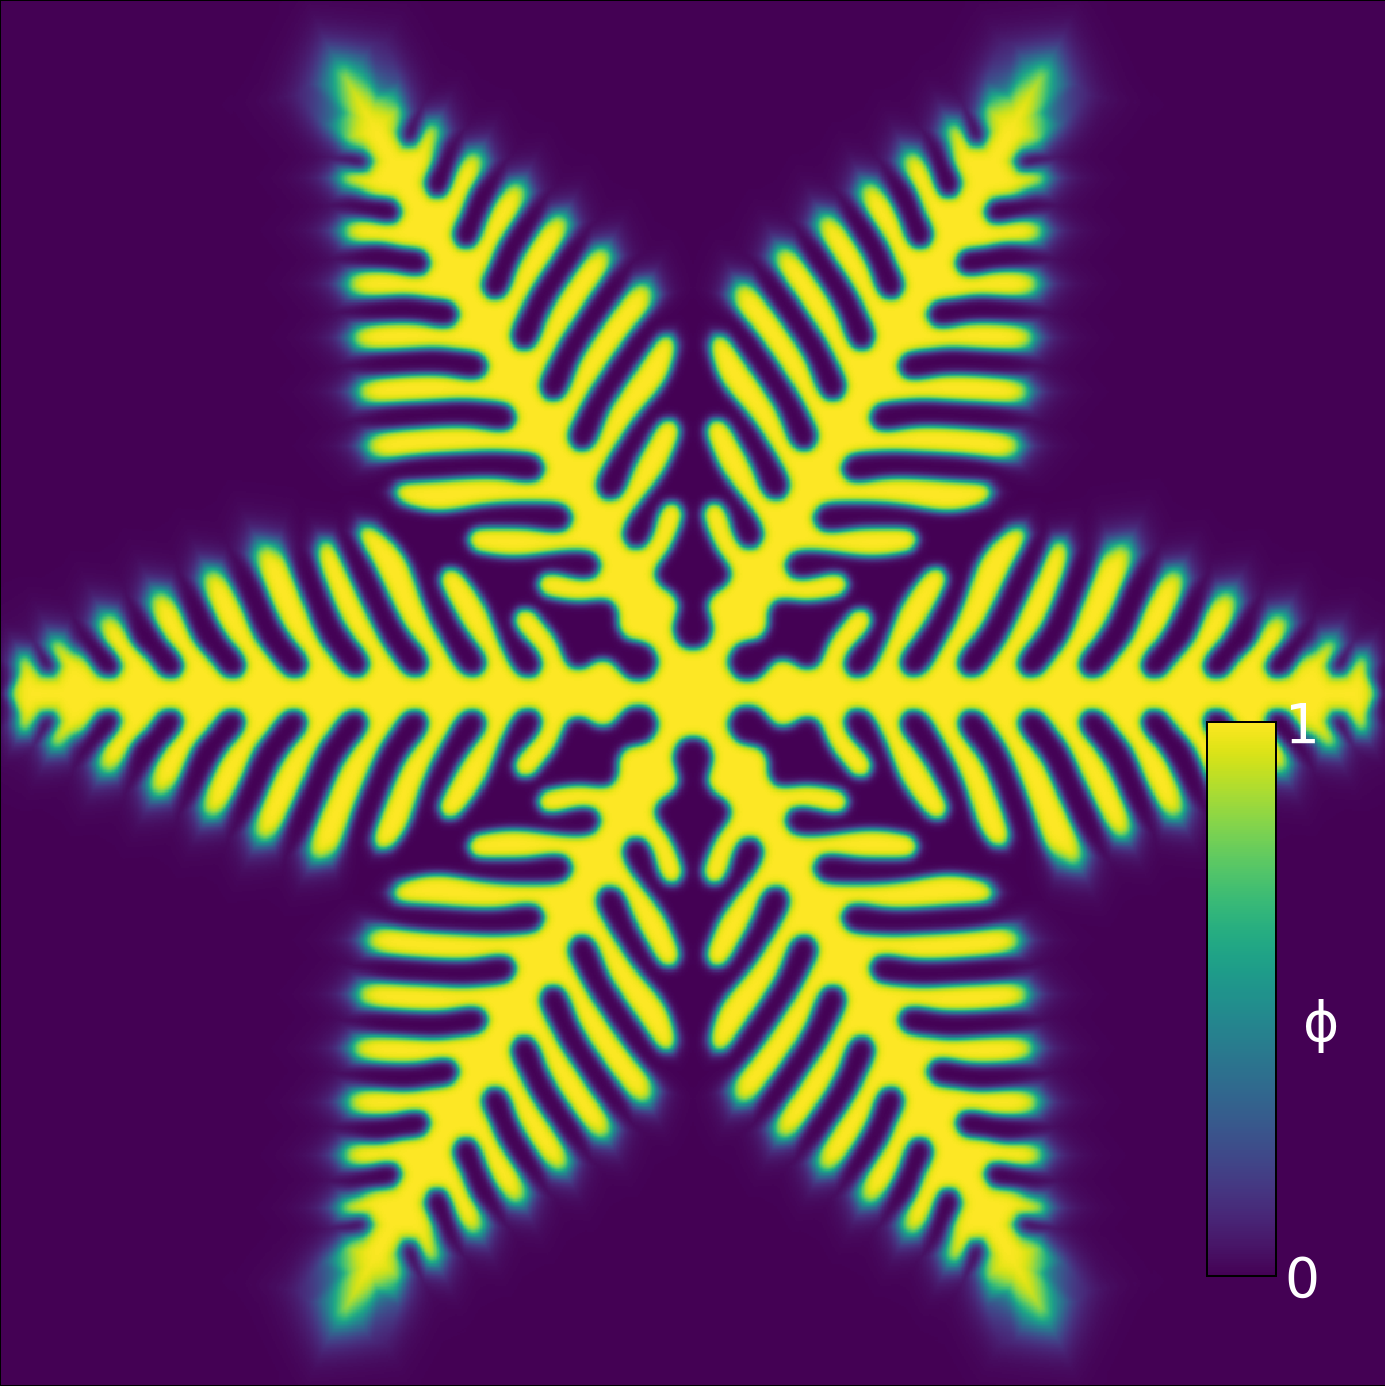
\includegraphics[width=\subfigwidth]{results/show_medium_xi_F_20.png}} \\
    
    \end{tabular}
    \caption{Comparison of phase fields for different values of parameter $\xi$ using the S-I scheme. Simulation setup given in Section \ref{sec:simulation setup} was used. Parameter $\xi$ was taken as one of $\{0.0025, 0.0043, 0.0065\}$. The width of the \emph{phase interface}, that is the region where the phase field $\Phi$ is between 0 and 1, is dependent on the value of $\xi$. For high value of $\xi = 0.0065$ the resulting phase field interface is thicker and heavily distorted in the direction of crystal growth. For medium values of $\xi = 0.0043$, roughly around the values of $\dx,\dy$, the phase field interface has the same thickness around the whole crystal. For small values of $\xi = 0.0025$, the proper shape of the phase interface cannot be accurately represented on the mesh, reducing the rate of crystal growth.
    }
    \label{fig:xi param results}
\end{figure}
\FloatBarrier


\FloatBarrier

\setlength{\subfigwidth}{0.29\textwidth}
\FloatBarrier
\begin{figure}[!ht]
    \centering
    \begin{tabular}{r P{\subfigwidth}P{\subfigwidth}P{\subfigwidth}}
    
    \rotatebox{90}{} & 
    $S = 0.0$ &
    $S = 0.3$ &
    $S = 0.5$ \\
    
    \rotatebox[origin=c]{90}{$t = 0.01$} & 
    \raisebox{-0.5\height}{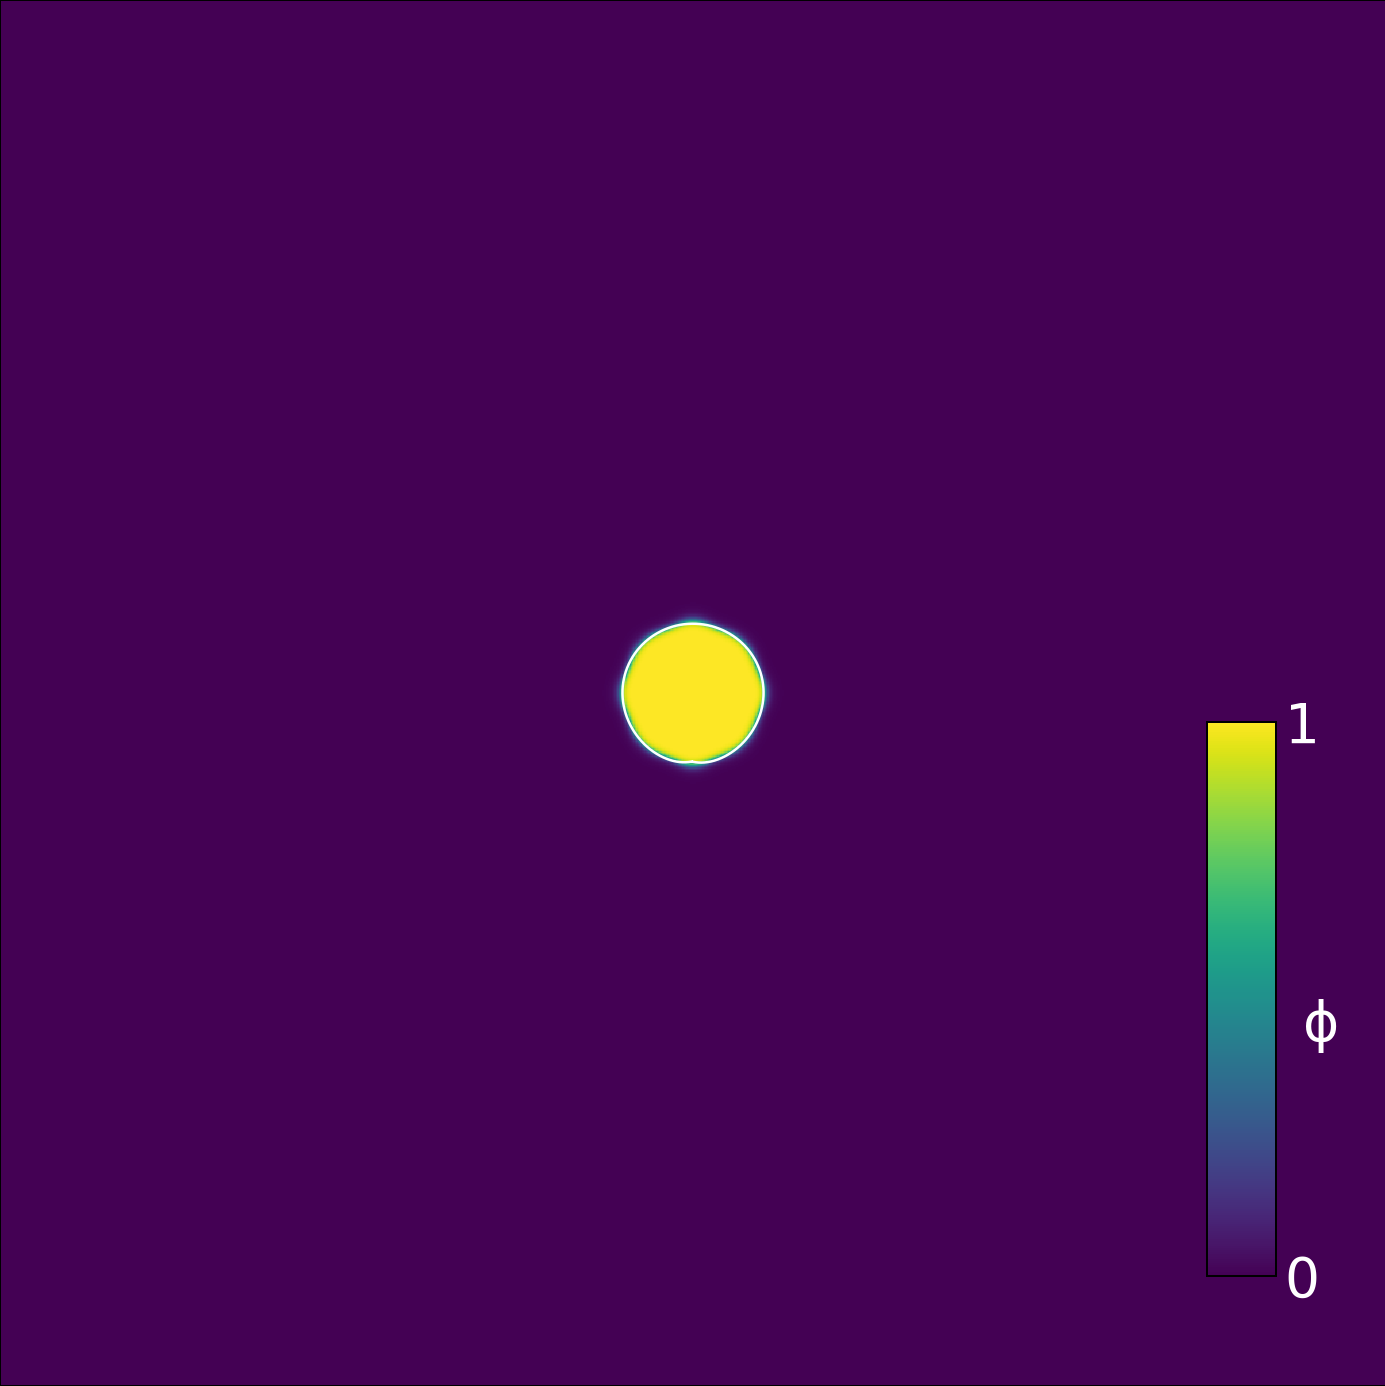
\includegraphics[width=\subfigwidth]{results/show_aniso_0_F_5.png}} &
    \raisebox{-0.5\height}{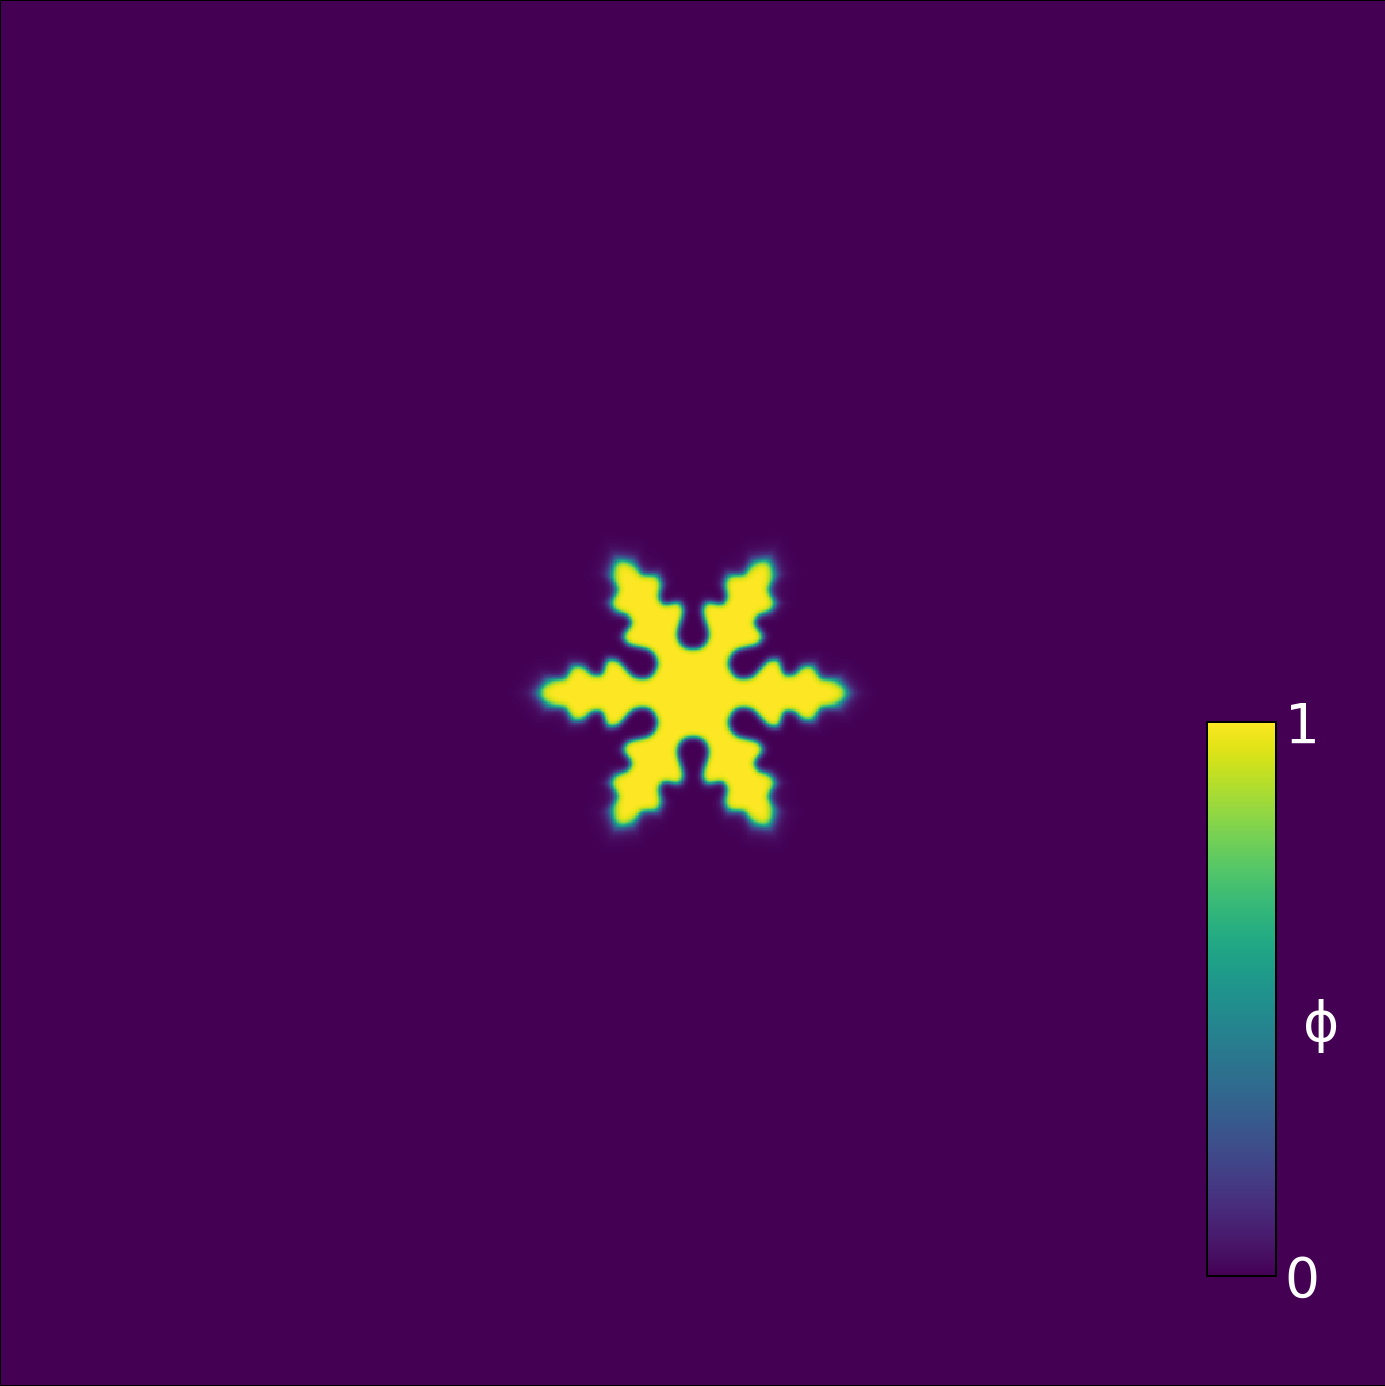
\includegraphics[width=\subfigwidth]{results/show_low_xi_F_5.png}} &
    \raisebox{-0.5\height}{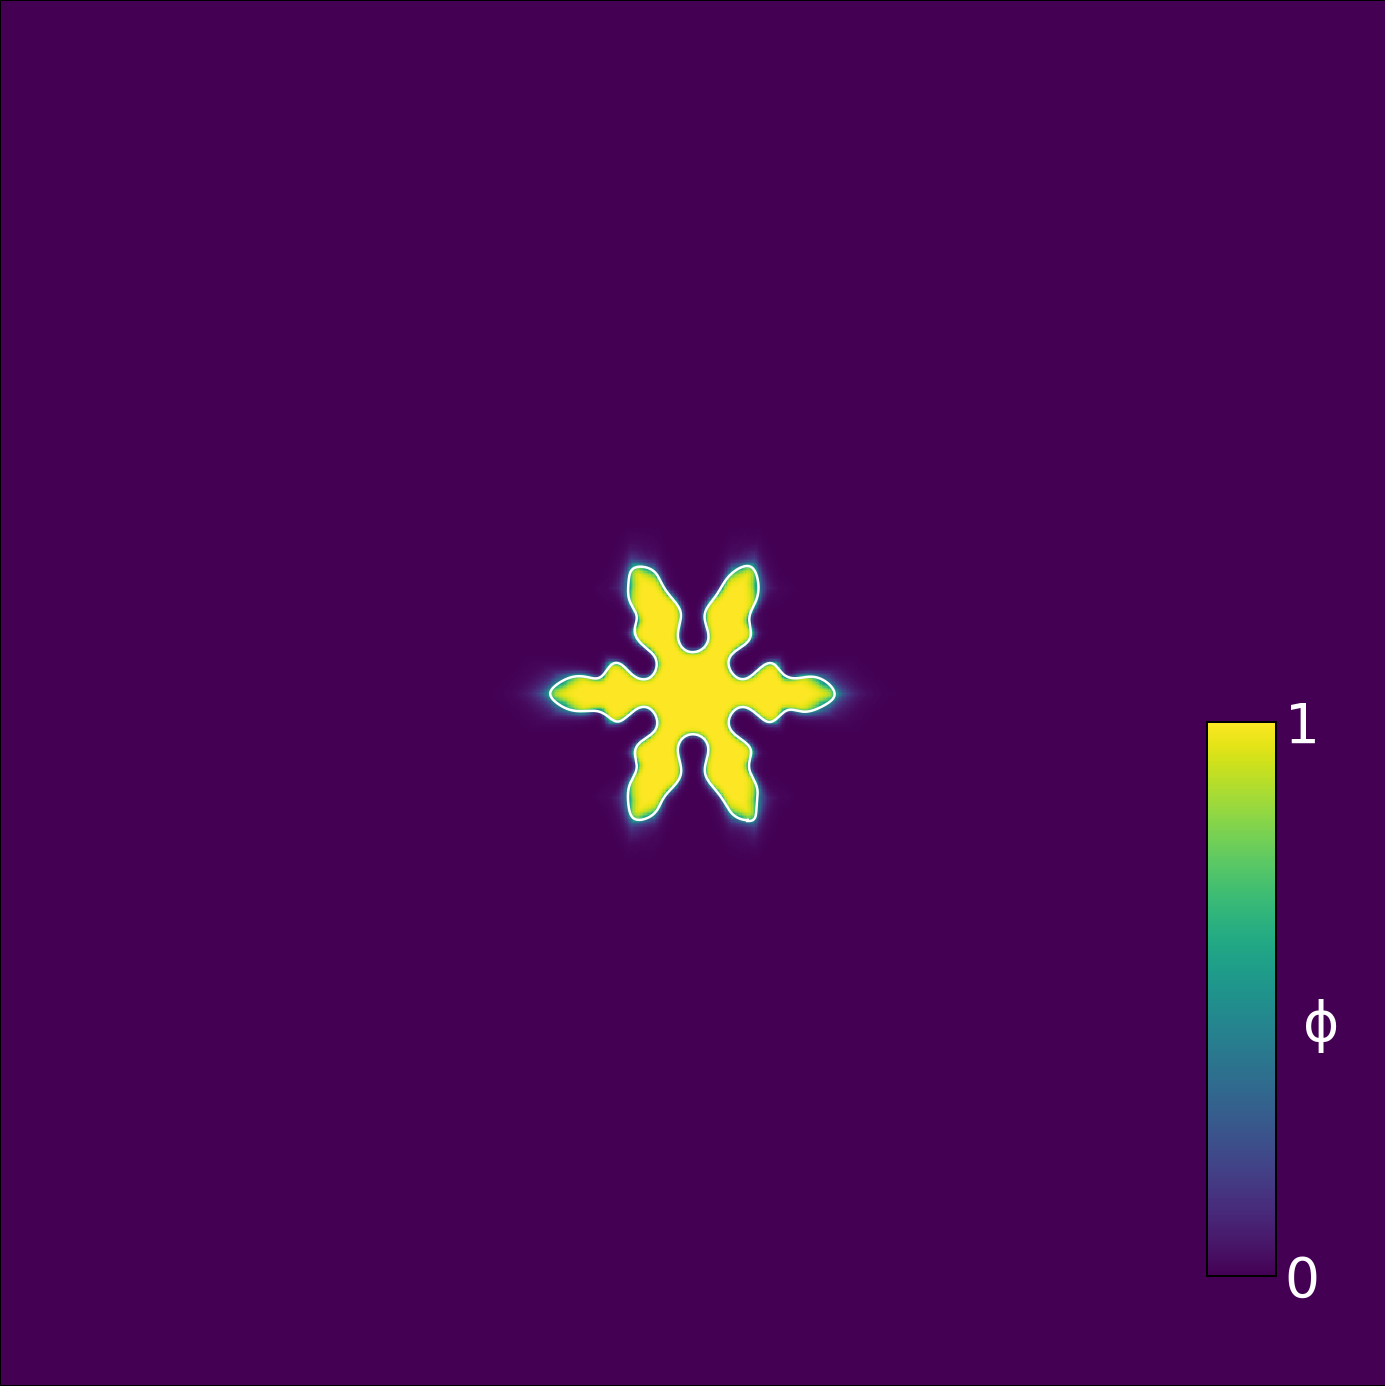
\includegraphics[width=\subfigwidth]{results/show_aniso_0.5_F_5.png}} \\
    \\
    \rotatebox[origin=c]{90}{$t = 0.0275$} & 
    \raisebox{-0.5\height}{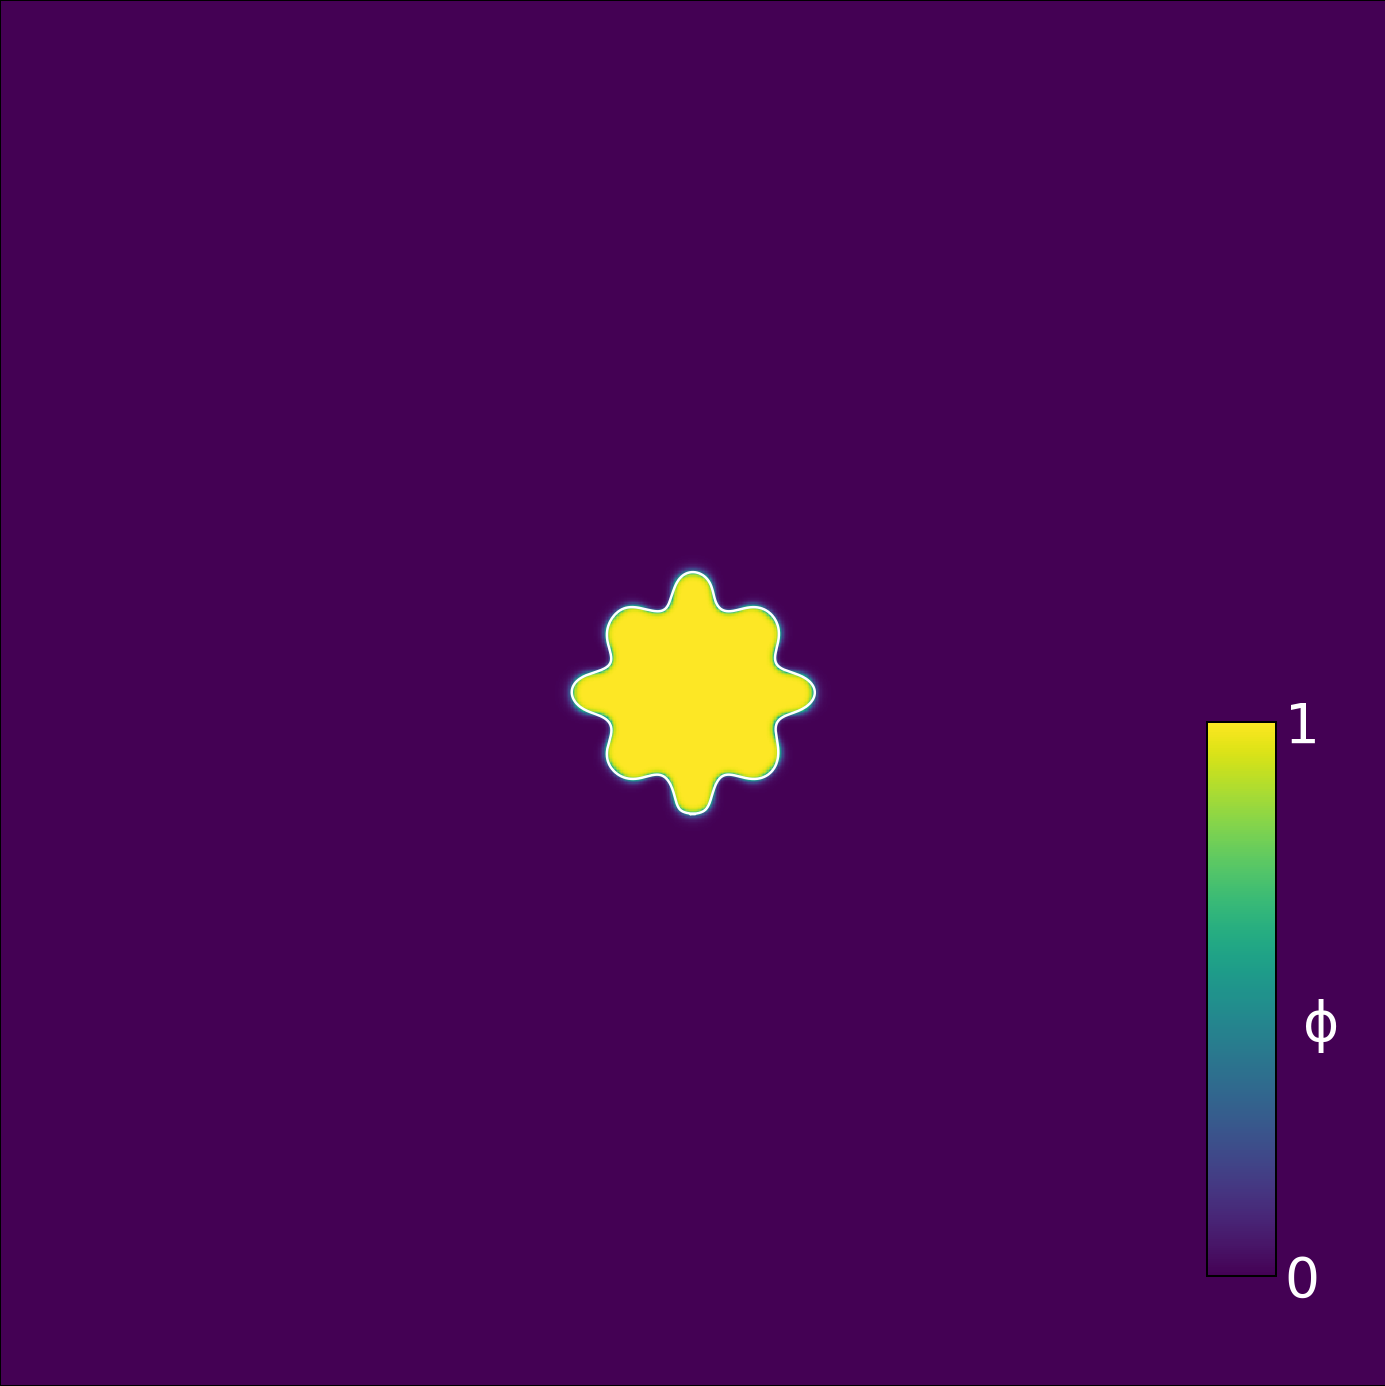
\includegraphics[width=\subfigwidth]{results/show_aniso_0_F_13.png}} &
    \raisebox{-0.5\height}{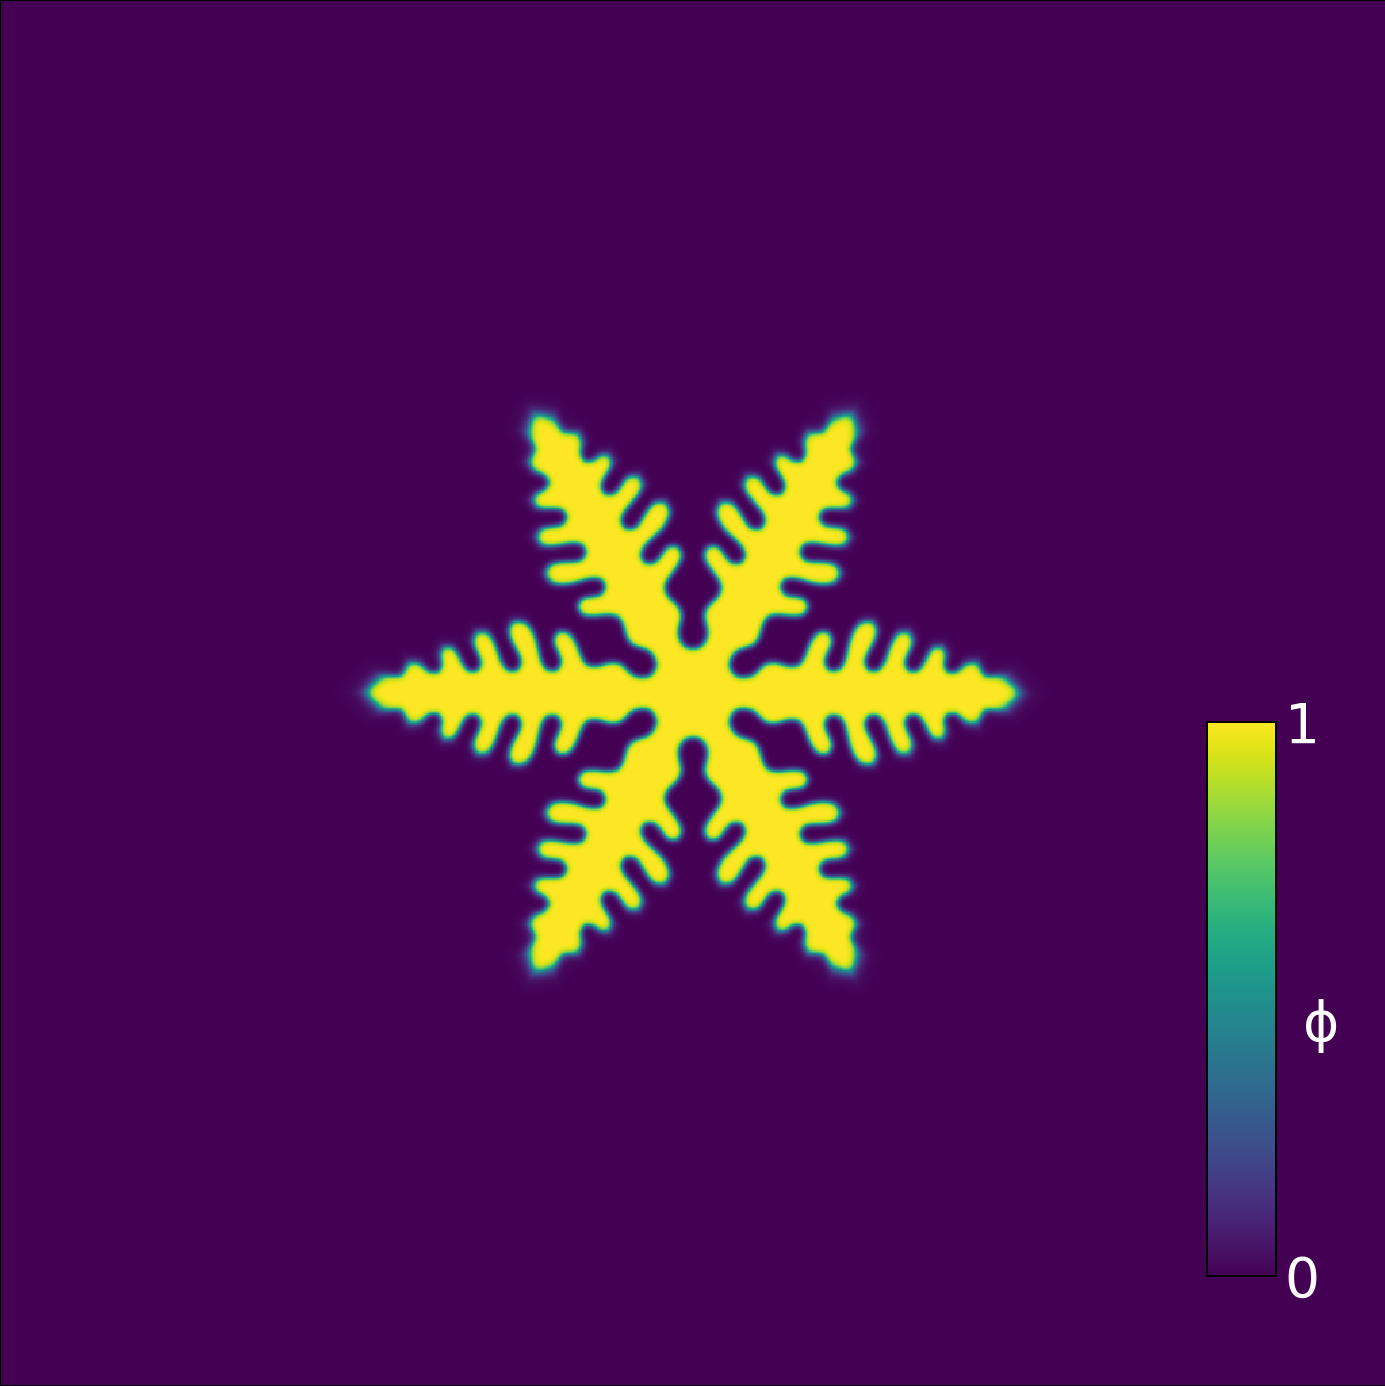
\includegraphics[width=\subfigwidth]{results/show_low_xi_F_13.png}} &
    \raisebox{-0.5\height}{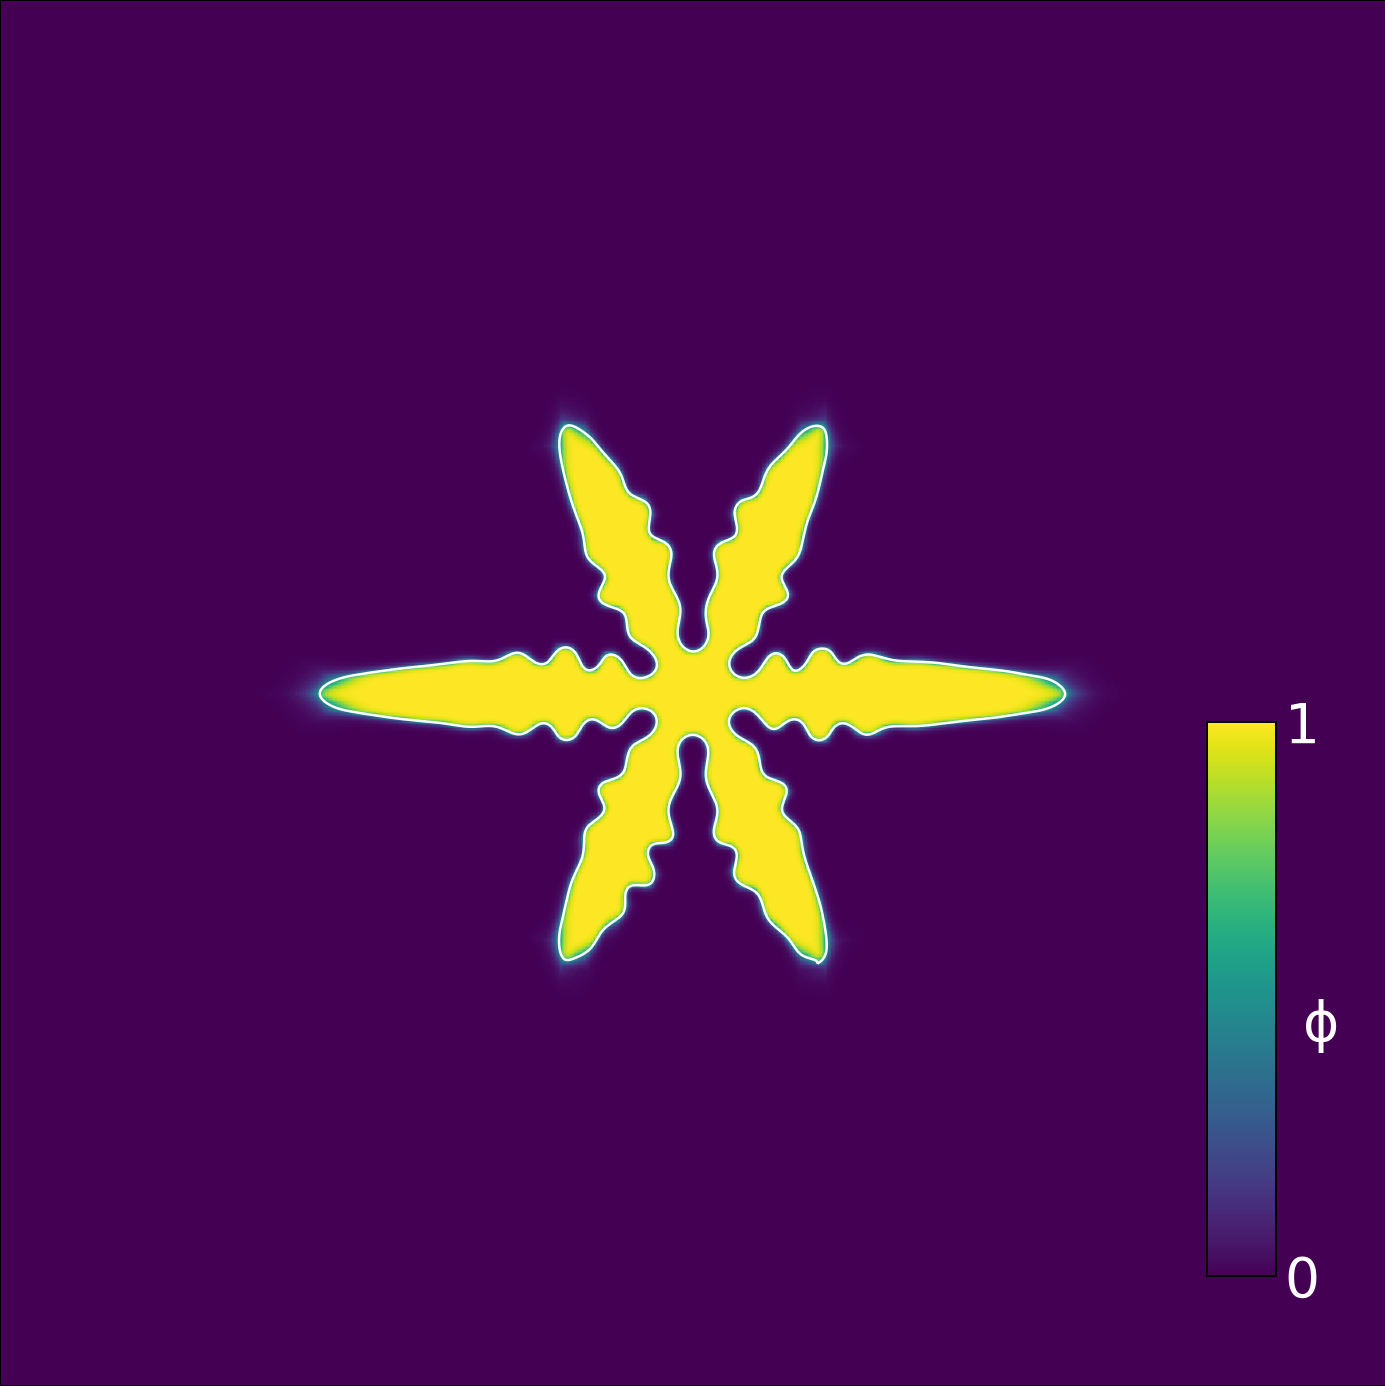
\includegraphics[width=\subfigwidth]{results/show_aniso_0.5_F_13.png}} \\
    \\
    \rotatebox[origin=c]{90}{$t = 0.04$} & 
    \raisebox{-0.5\height}{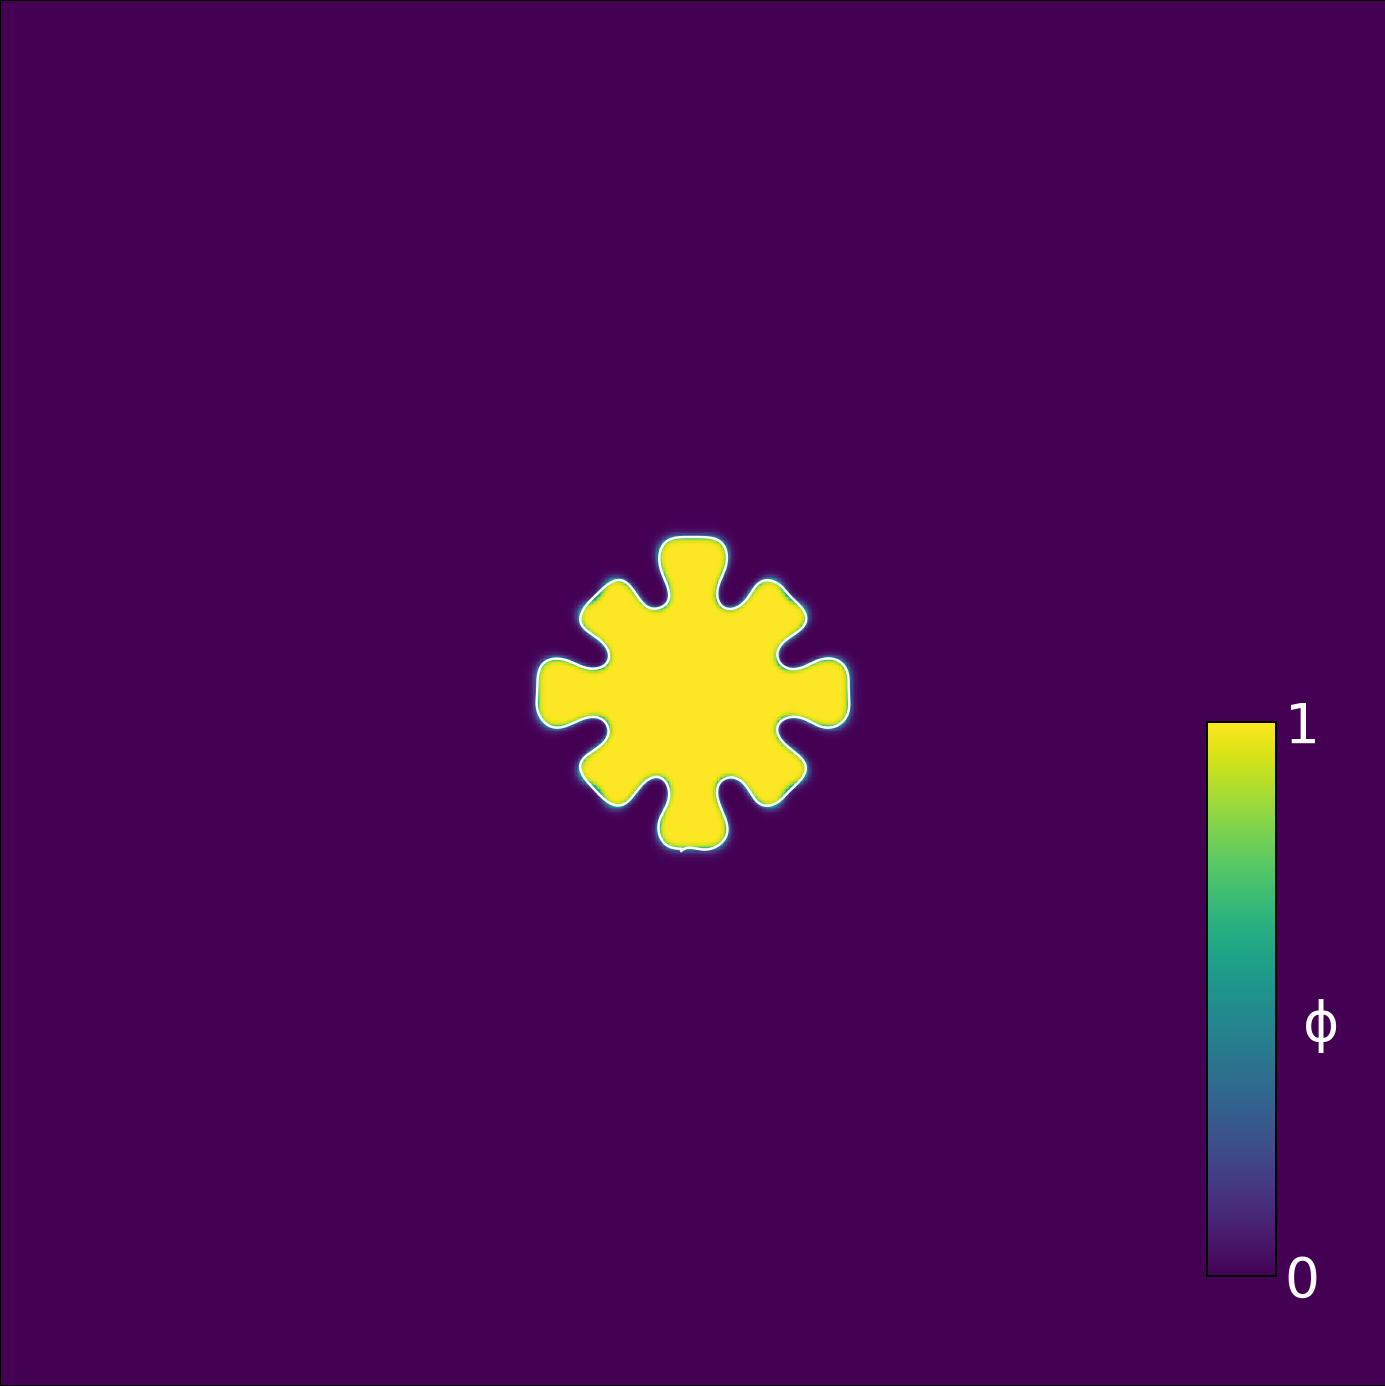
\includegraphics[width=\subfigwidth]{results/show_aniso_0_F_20.png}} &
    \raisebox{-0.5\height}{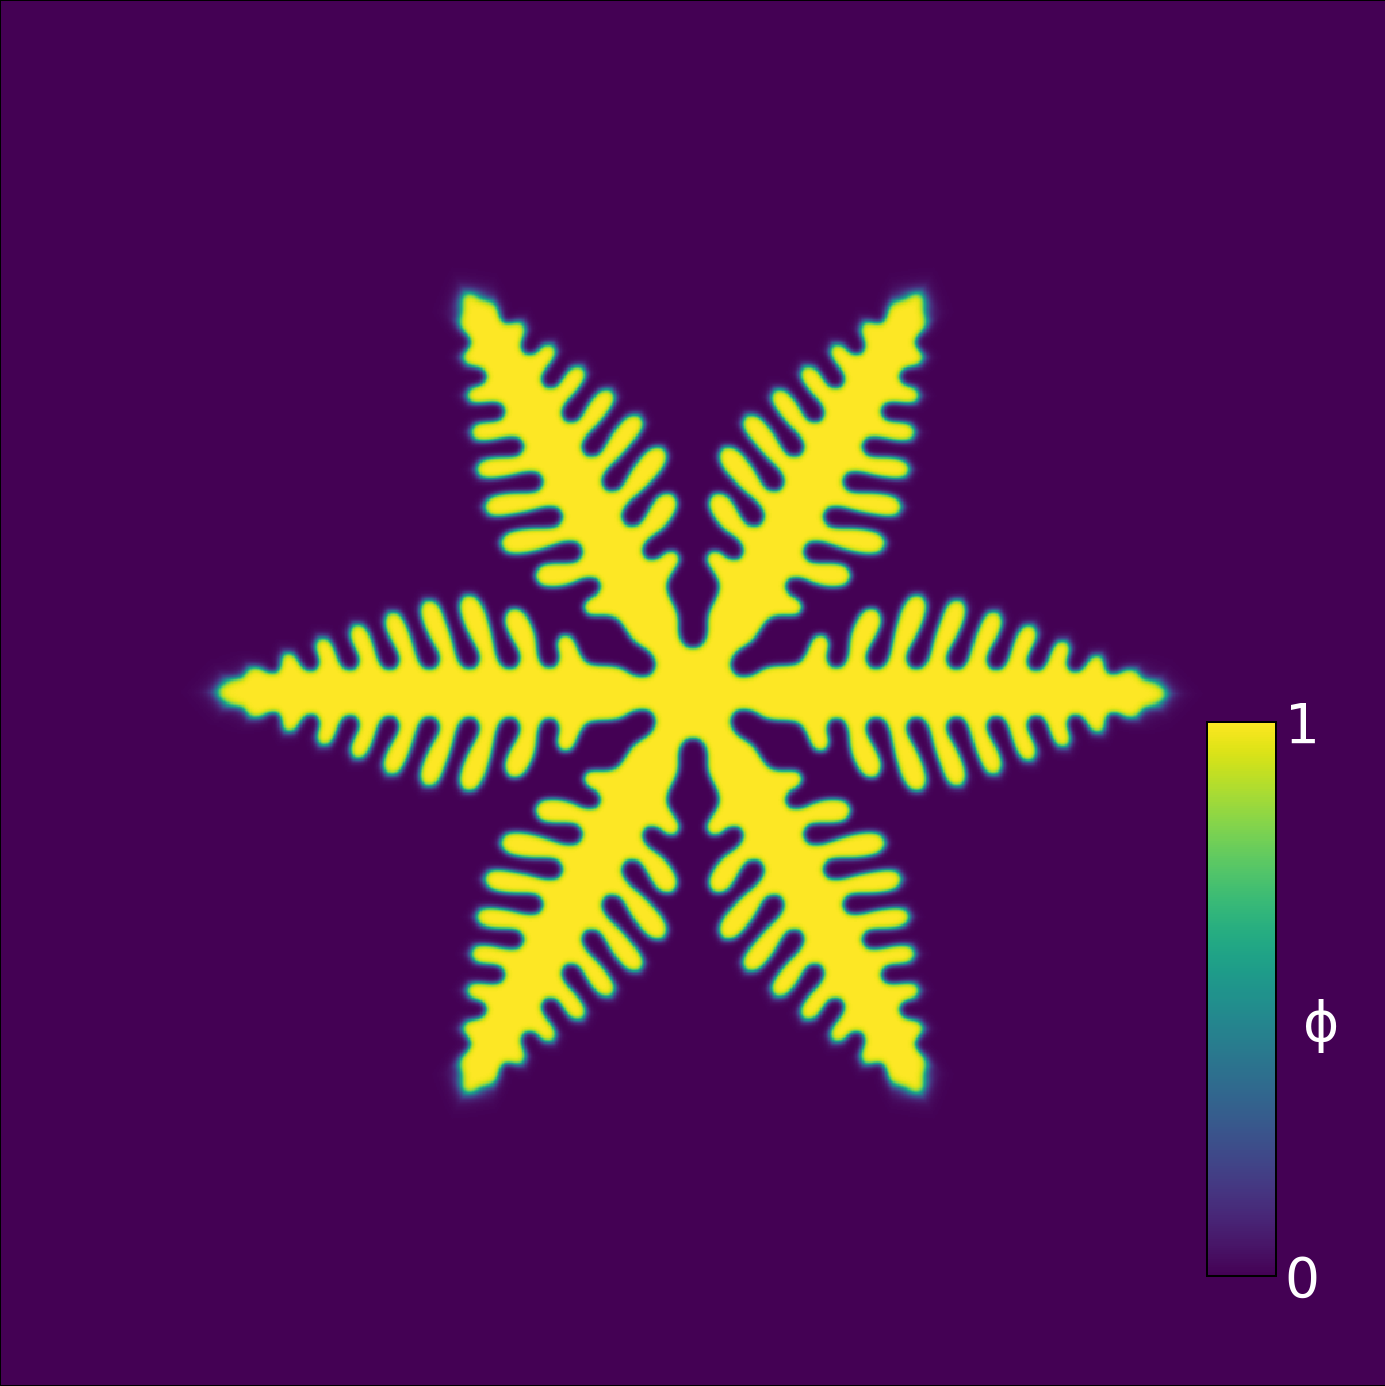
\includegraphics[width=\subfigwidth]{results/show_low_xi_F_20.png}} &
    \raisebox{-0.5\height}{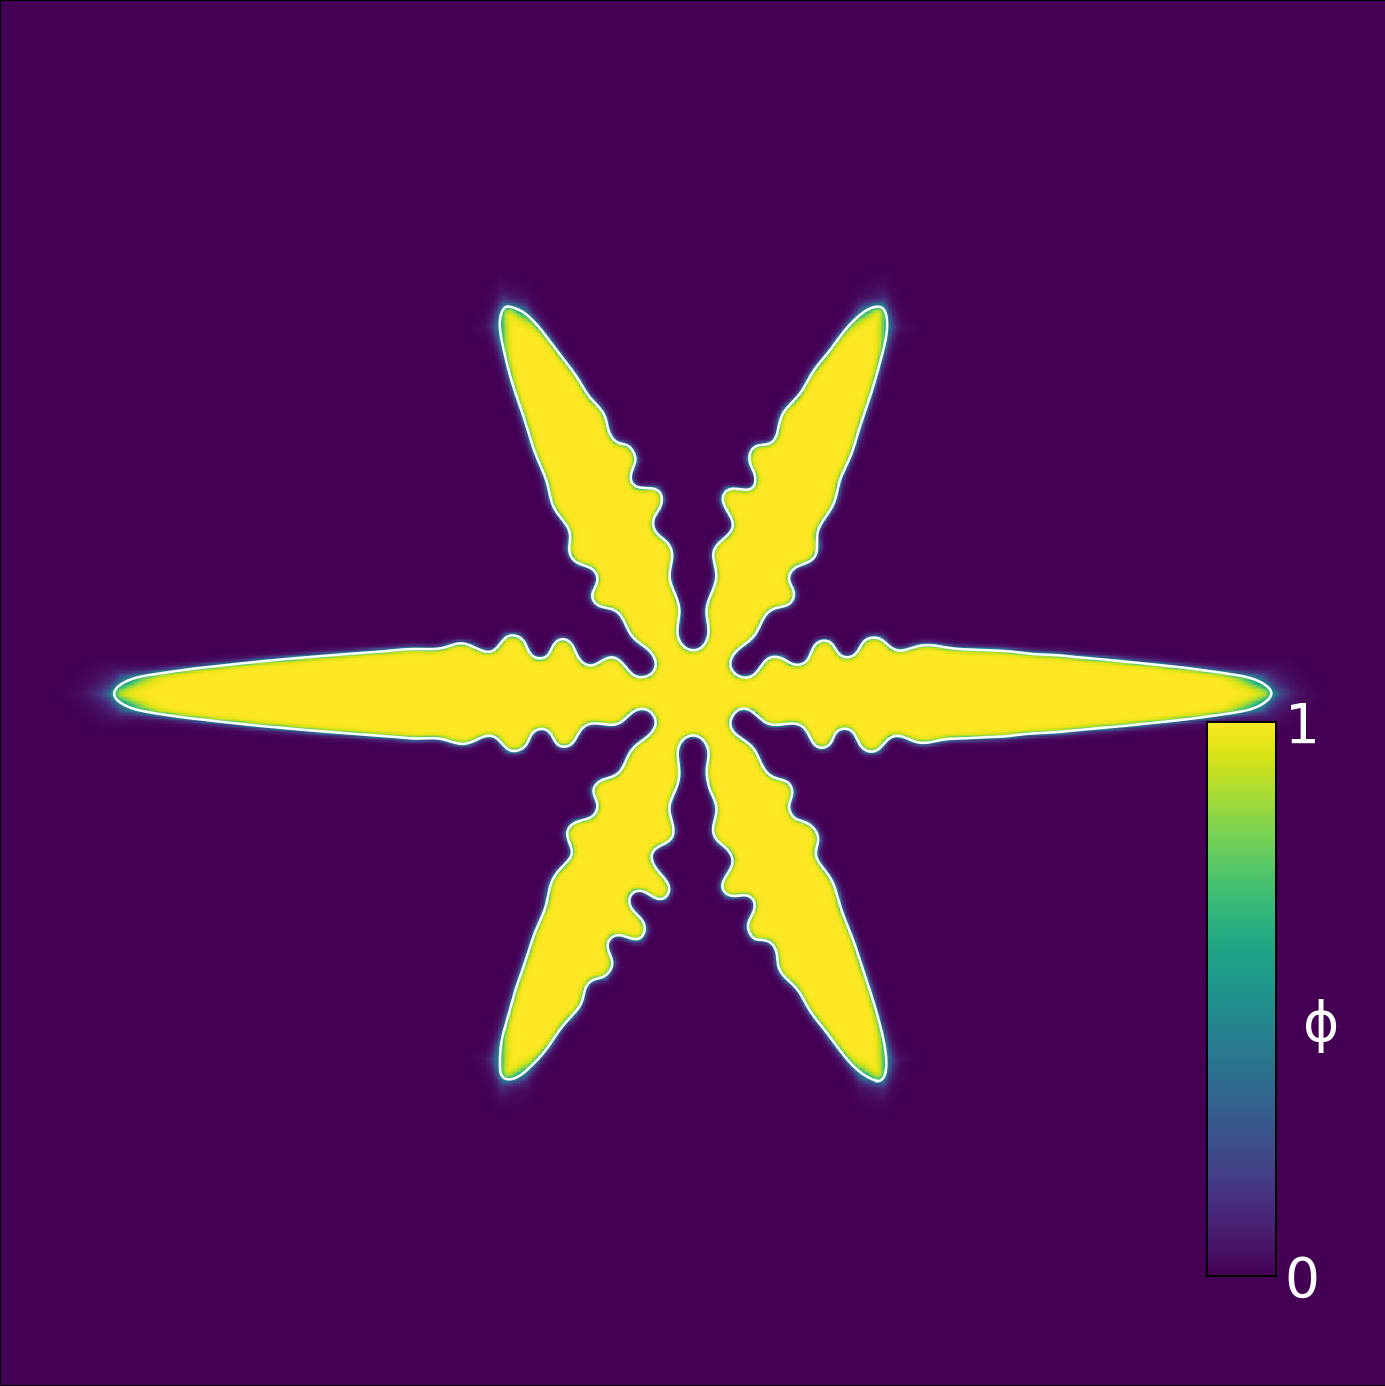
\includegraphics[width=\subfigwidth]{results/show_aniso_0.5_F_20.png}} \\
    
    \end{tabular}
        \caption{Comparison of phase fields for different values of anisotropy strength $S$ using the S-I scheme. Simulation setup given in Section \ref{sec:simulation setup} was used. $S$ was taken as one of $\{0, 0.3, 0.5\}$. For low and high values of anisotropy strength, the underlying regular grid has a visible impact on the resulting crystal structure. Specifically in the case of $S = 0$, the crystal should remain a perfect ball.
    }
    \label{fig:aniso param results}
\end{figure}
\FloatBarrier


\setlength{\subfigwidth}{0.31\textwidth}
\FloatBarrier
\begin{figure}[!ht]
    \centering
    \begin{tabular}{P{\subfigwidth}P{\subfigwidth}P{\subfigwidth}}
    
    {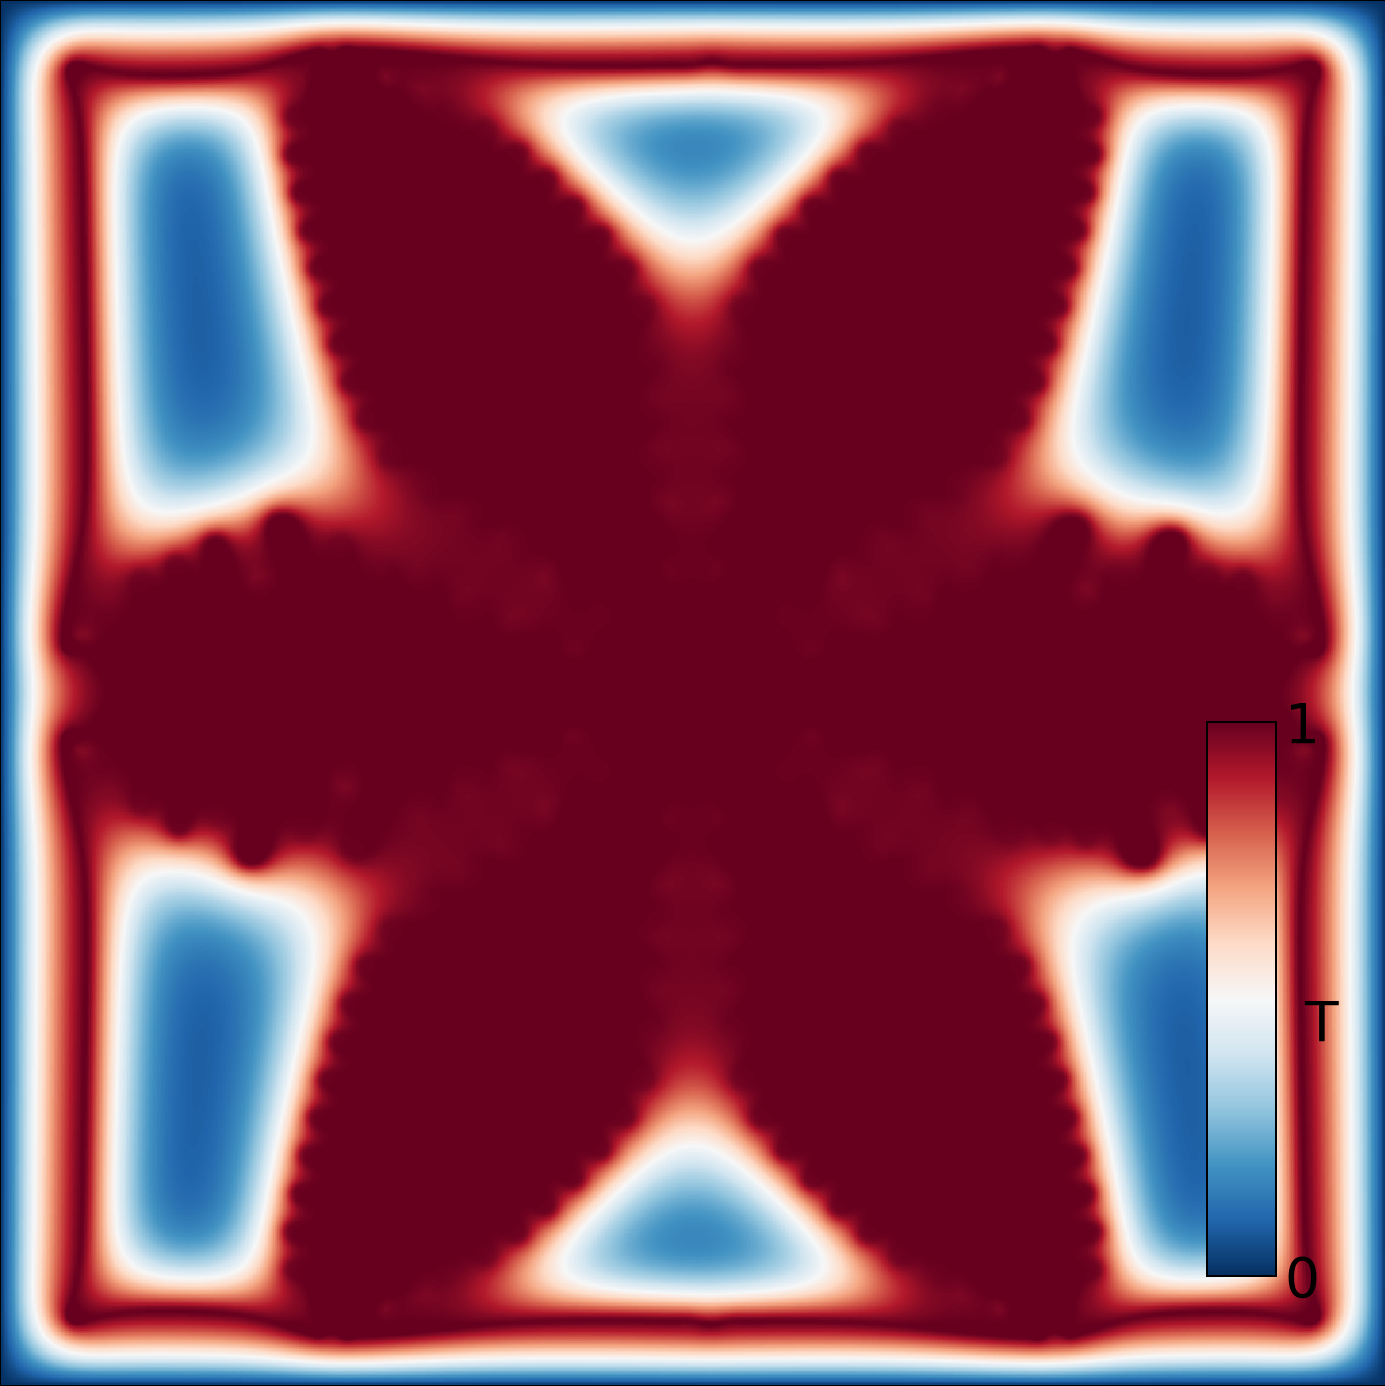
\includegraphics[width=\subfigwidth]{results/semi_long_dirichlet_U_10.png}} &
    {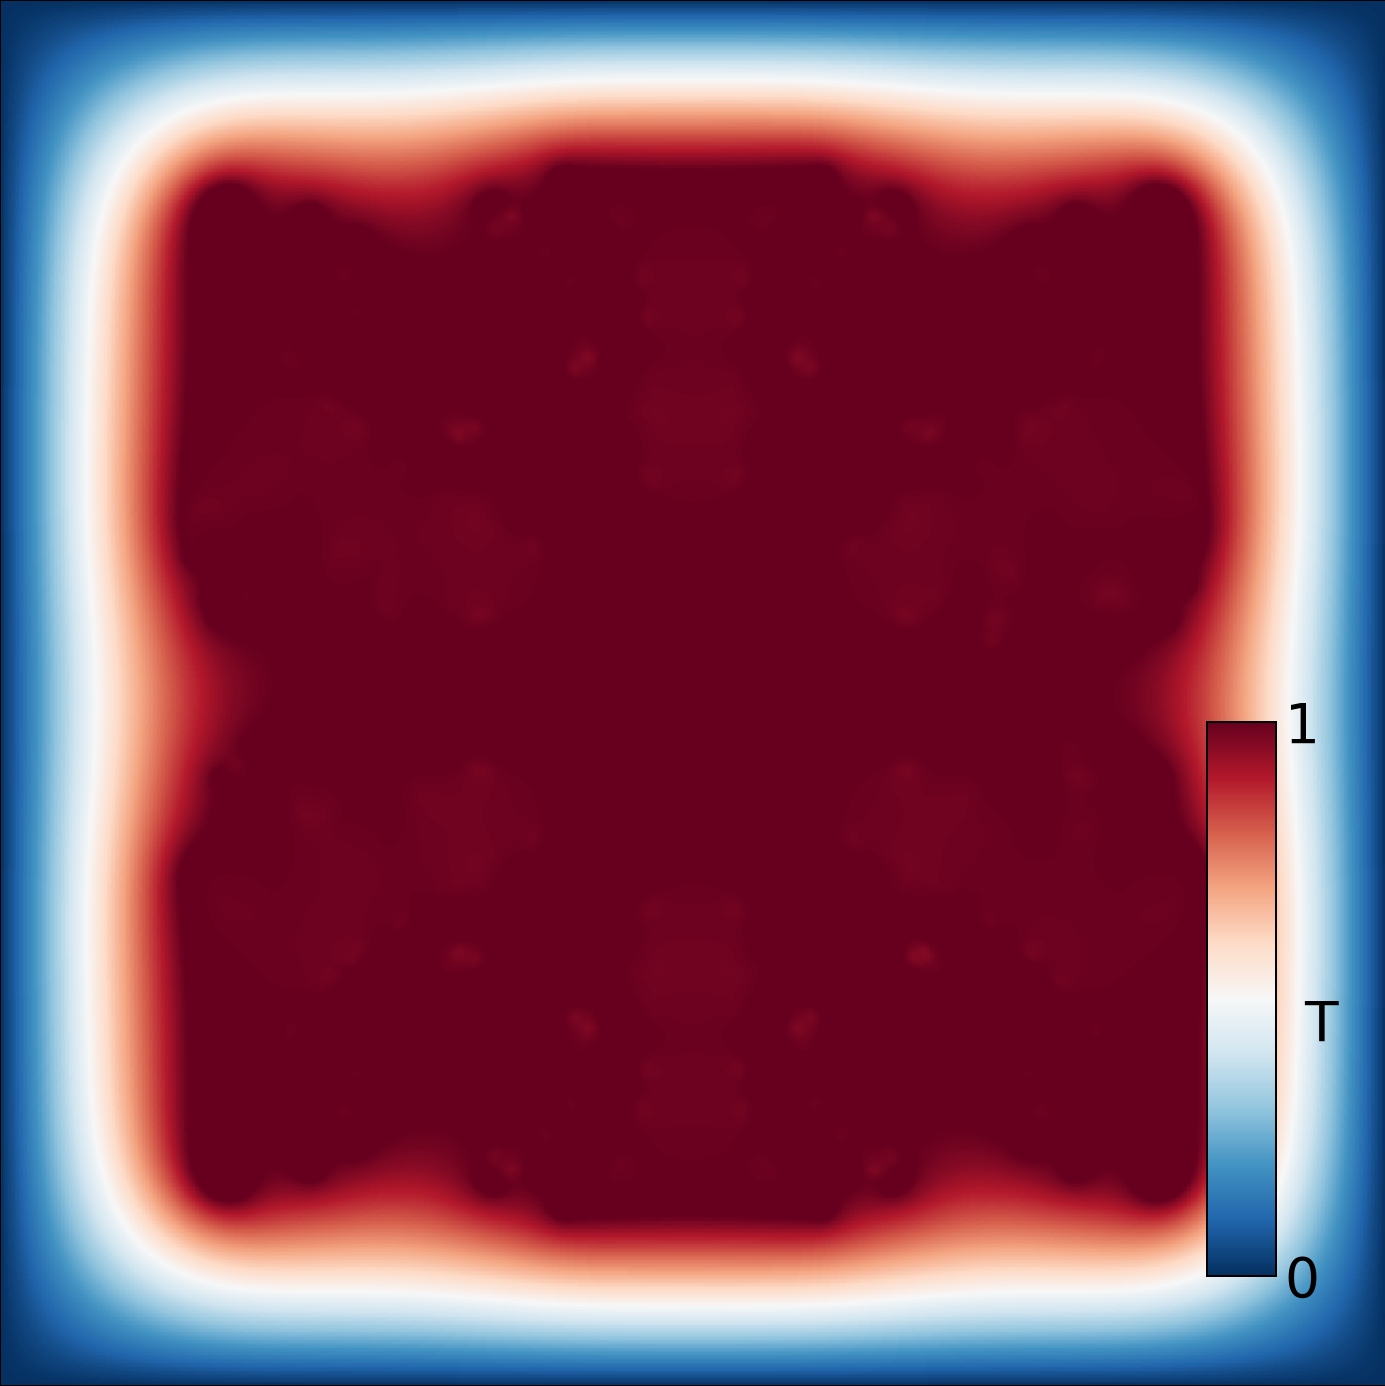
\includegraphics[width=\subfigwidth]{results/semi_long_dirichlet_U_30.png}} &
    {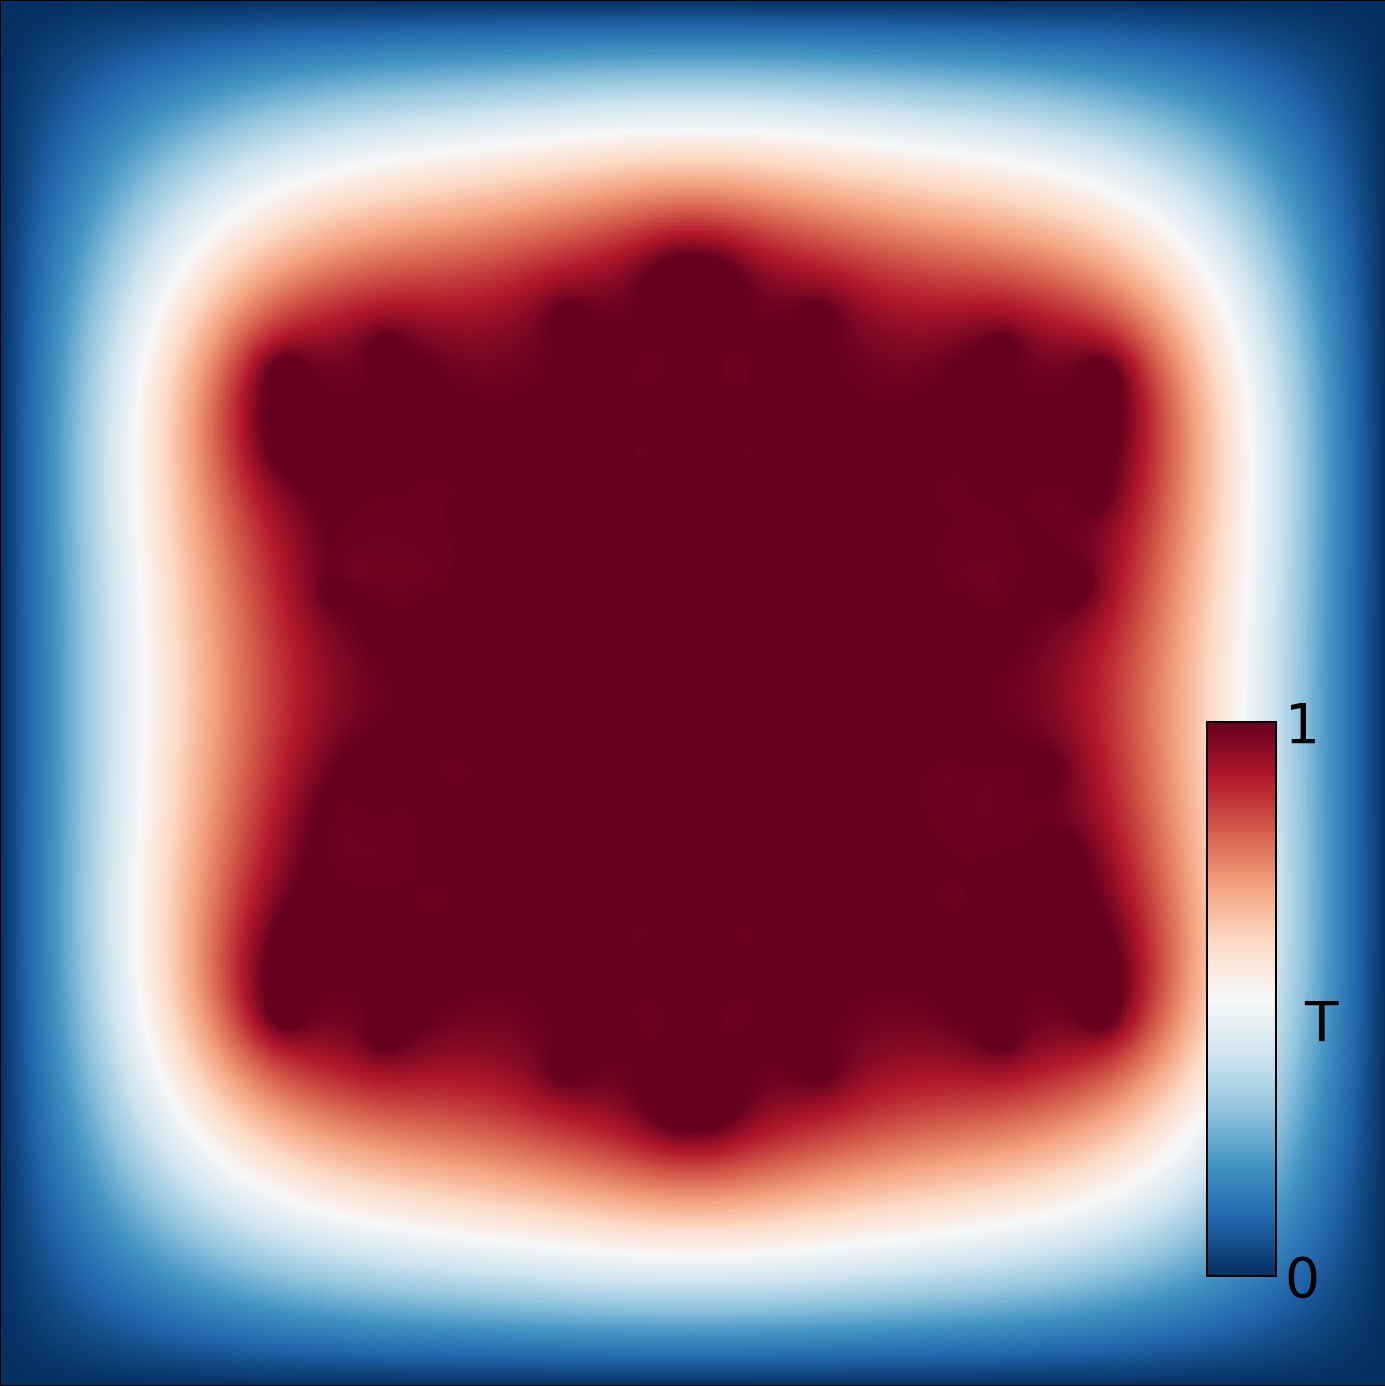
\includegraphics[width=\subfigwidth]{results/semi_long_dirichlet_U_60.png}} \\
    \\
    {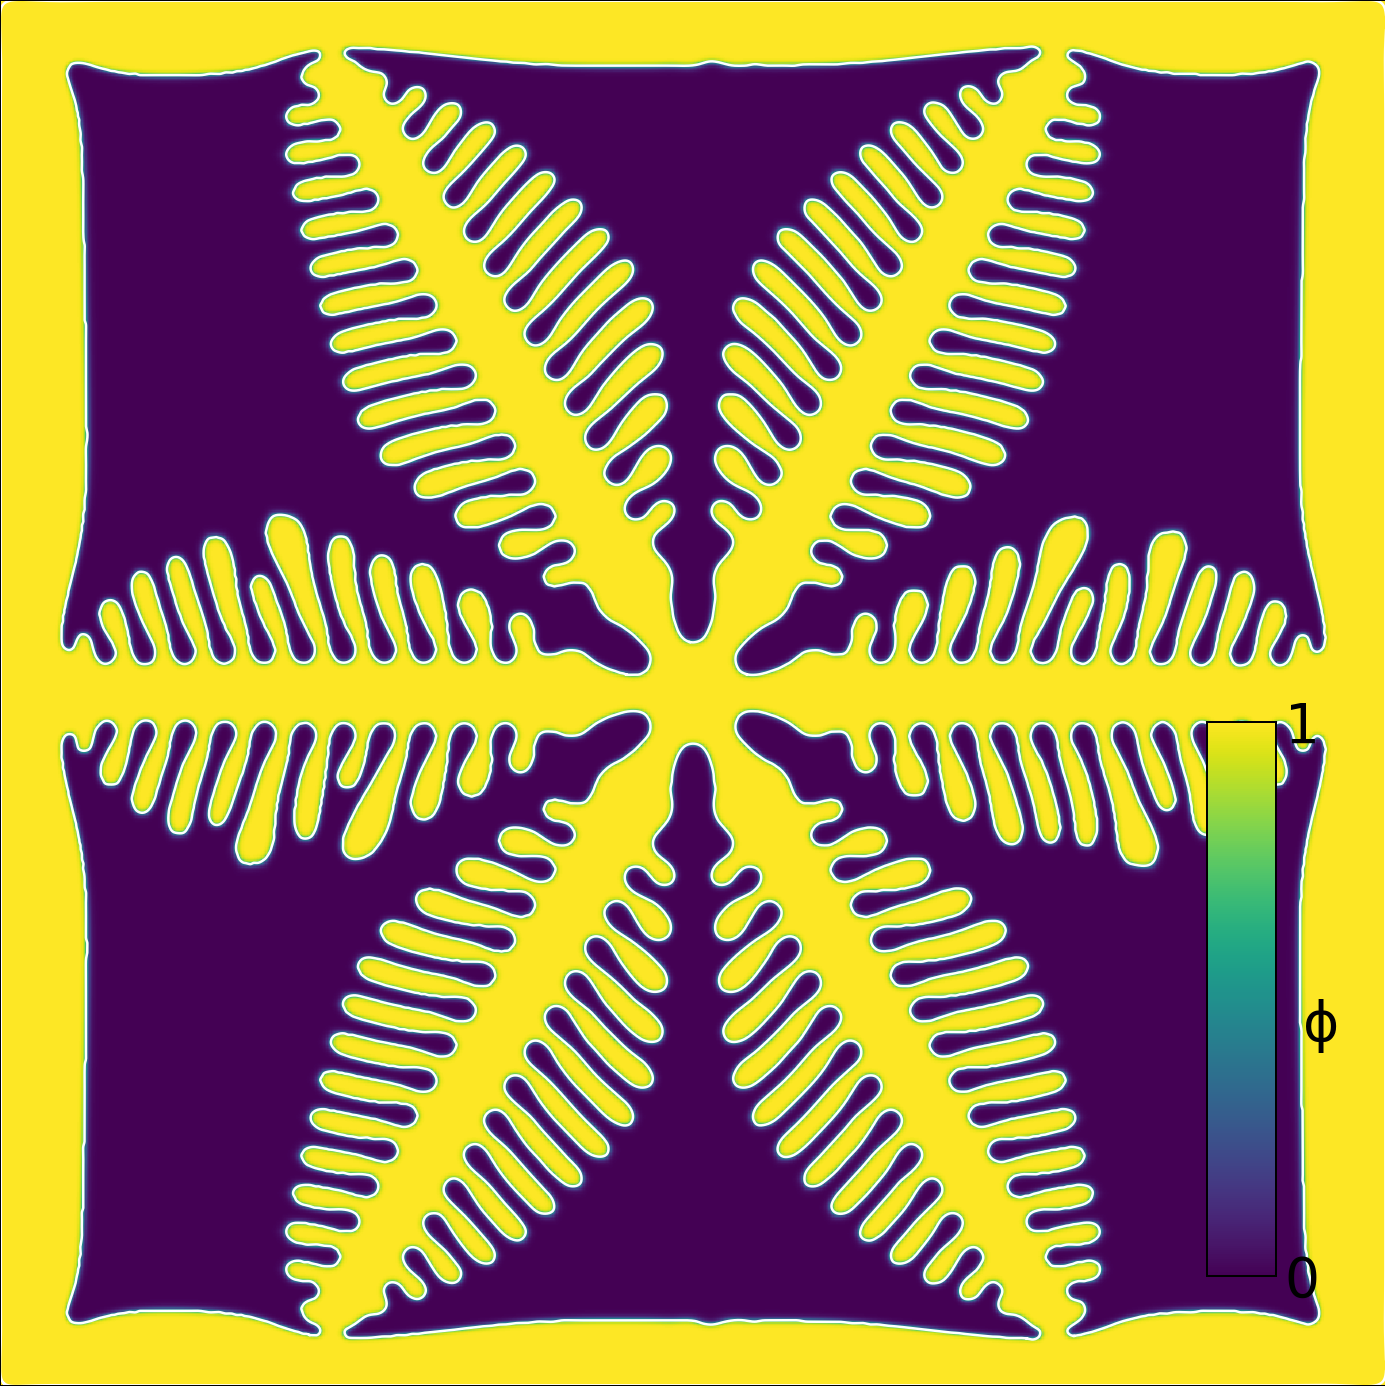
\includegraphics[width=\subfigwidth]{results/semi_long_dirichlet_F_10.png}} &
    {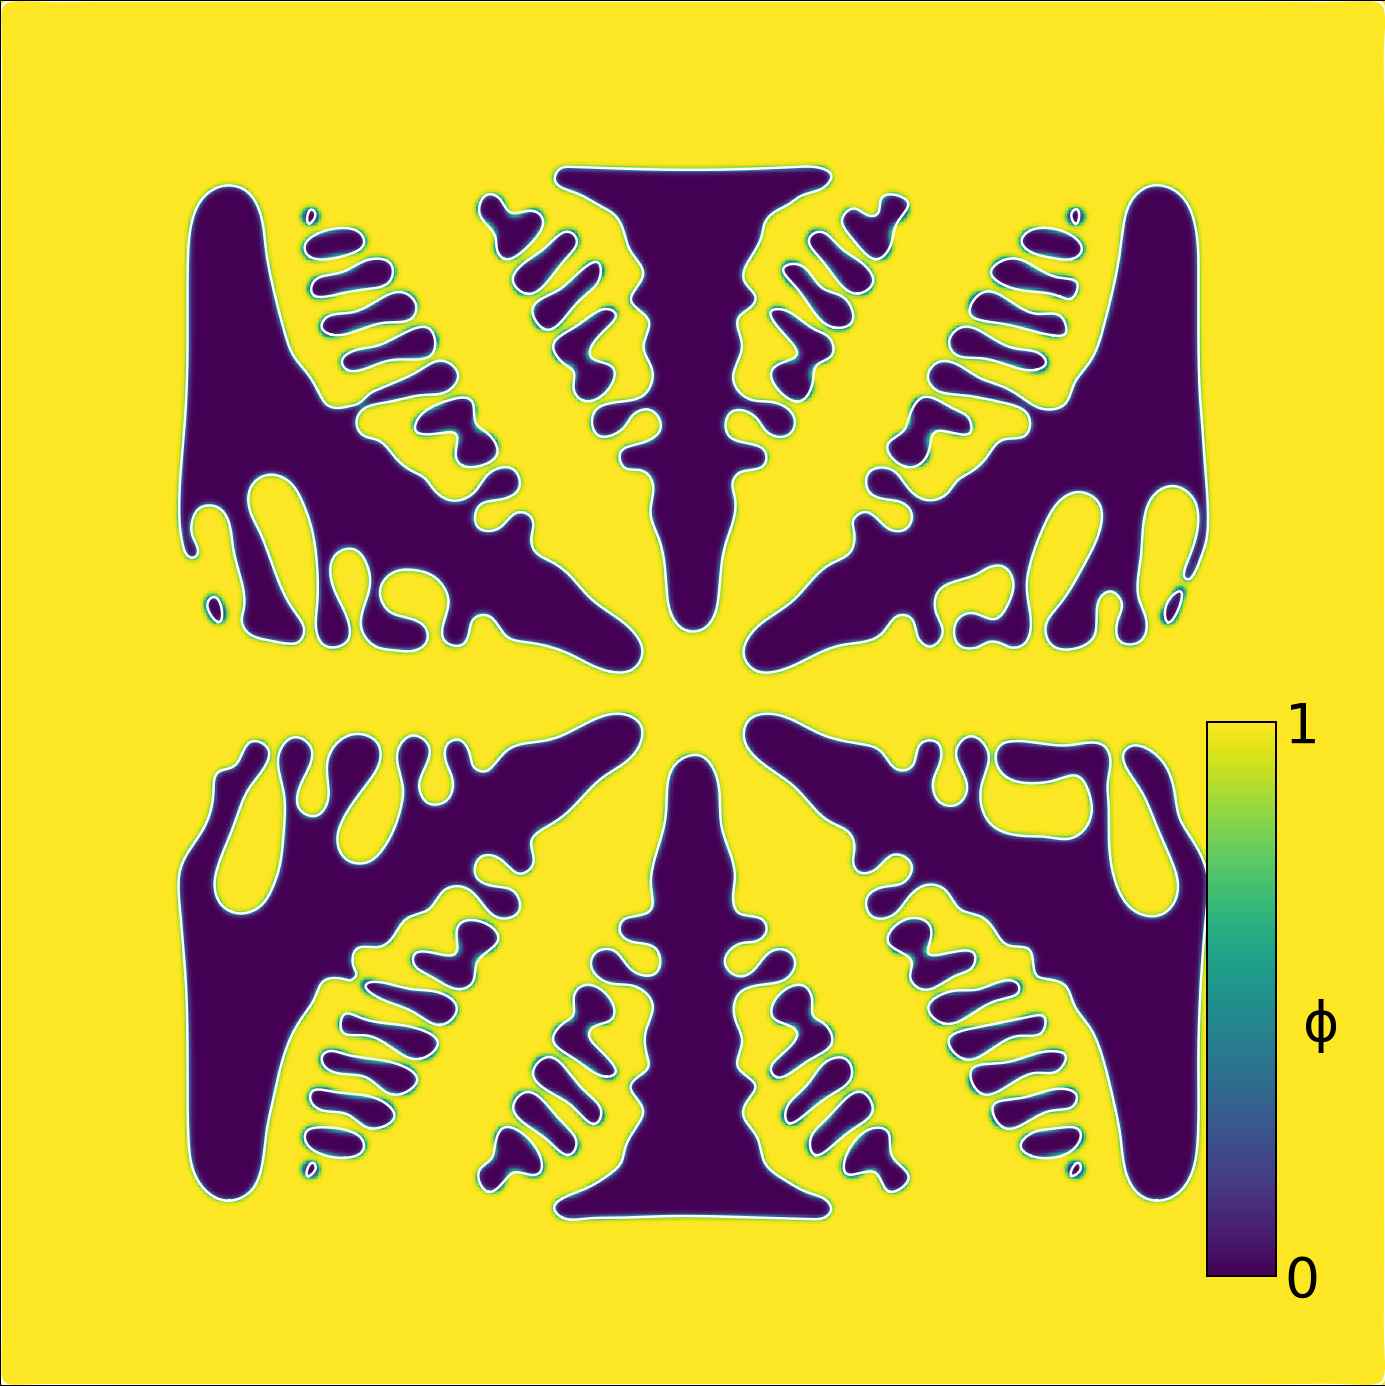
\includegraphics[width=\subfigwidth]{results/semi_long_dirichlet_F_30.png}} &
    {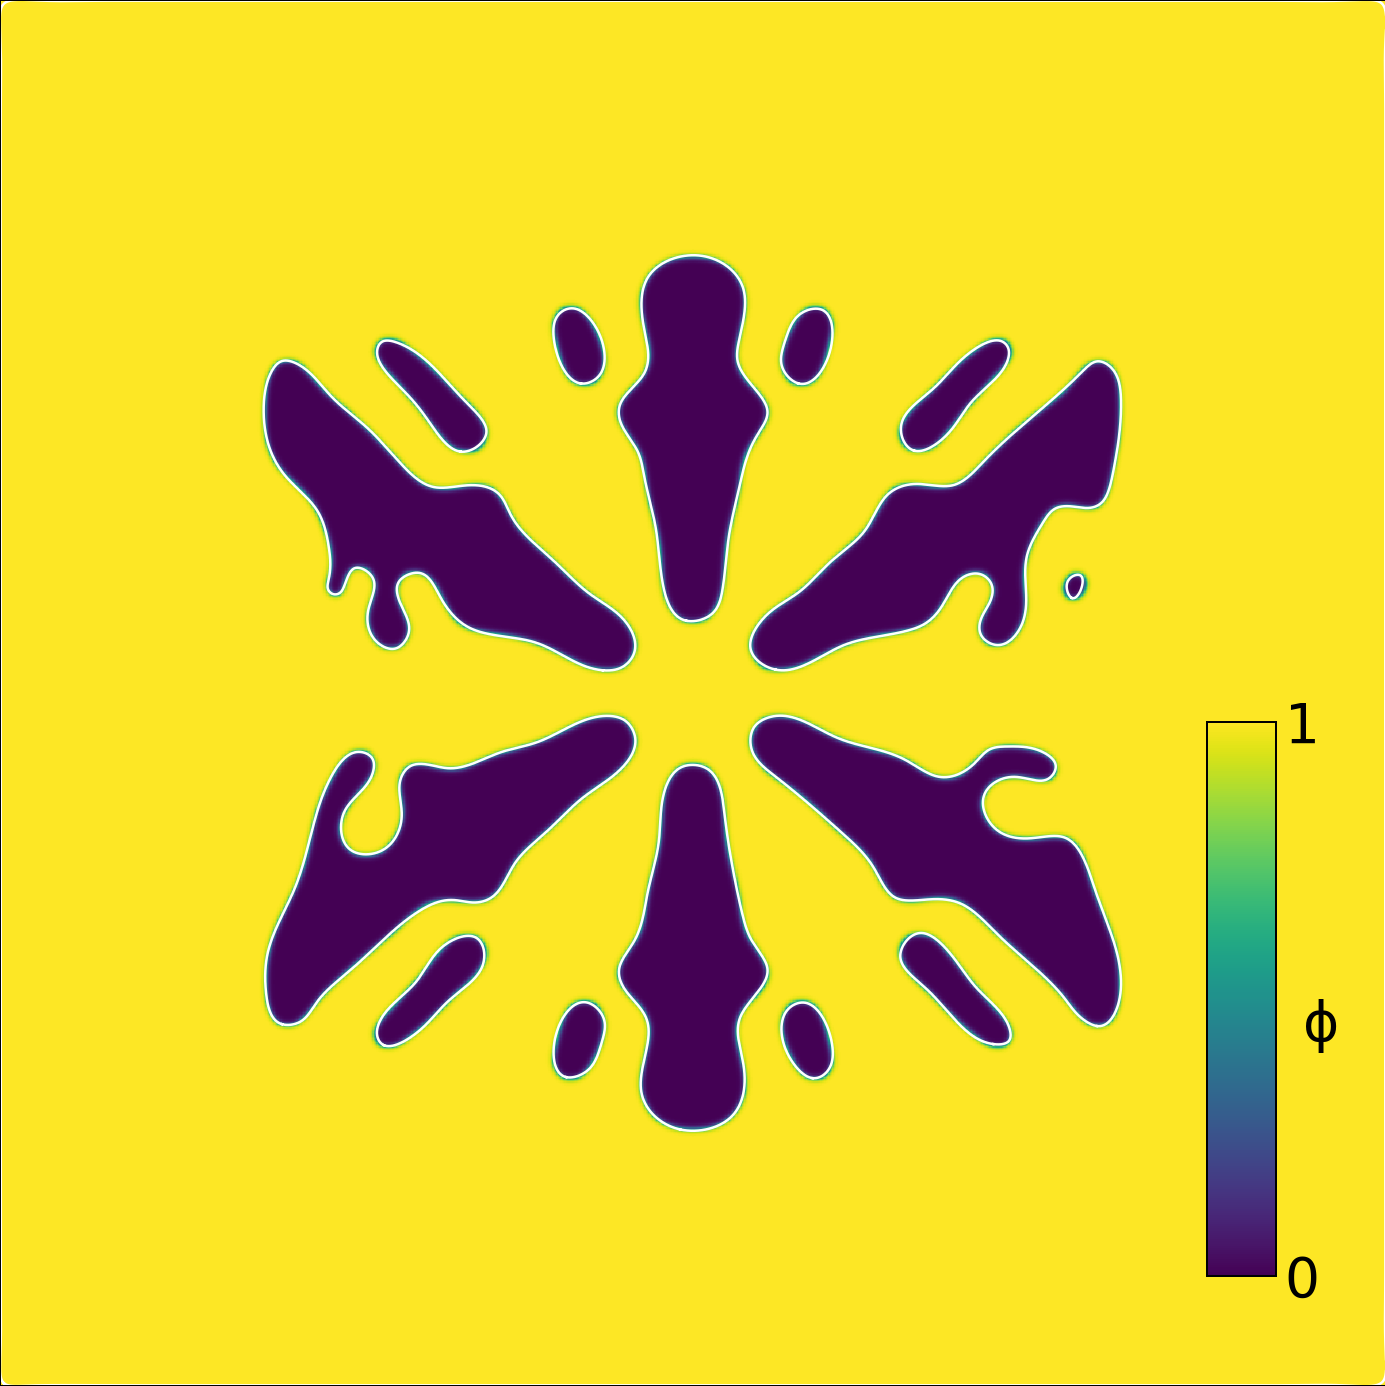
\includegraphics[width=\subfigwidth]{results/semi_long_dirichlet_F_60.png}} \\
    $t = 0.1$ & 
    $t = 0.3$ &
    $t = 0.6$ 
    
    \end{tabular}
    \caption{
        Evolution of the temperature field $T$ (top) and the phase field $\Phi$ (bottom) over the time interval $\Timeint = [0, 0.6]$ using the S-I scheme. Simulation setup given in Section \ref{sec:simulation setup} alongside Dirichlet boundary conditions for the the temperature field (\ref{eq:dirichlet T boundary conditions}) were used. Due to the controlled cooling at the boundary, the crystal expands, eventually filling the entire domain $\Omega$.
    }
    \label{fig:def params results 8 an}
\end{figure}
\FloatBarrier

\setlength{\subfigwidth}{0.31\textwidth}
\FloatBarrier
\begin{figure}[!ht]
    \centering
    \begin{tabular}{P{\subfigwidth}P{\subfigwidth}P{\subfigwidth}}
    
    {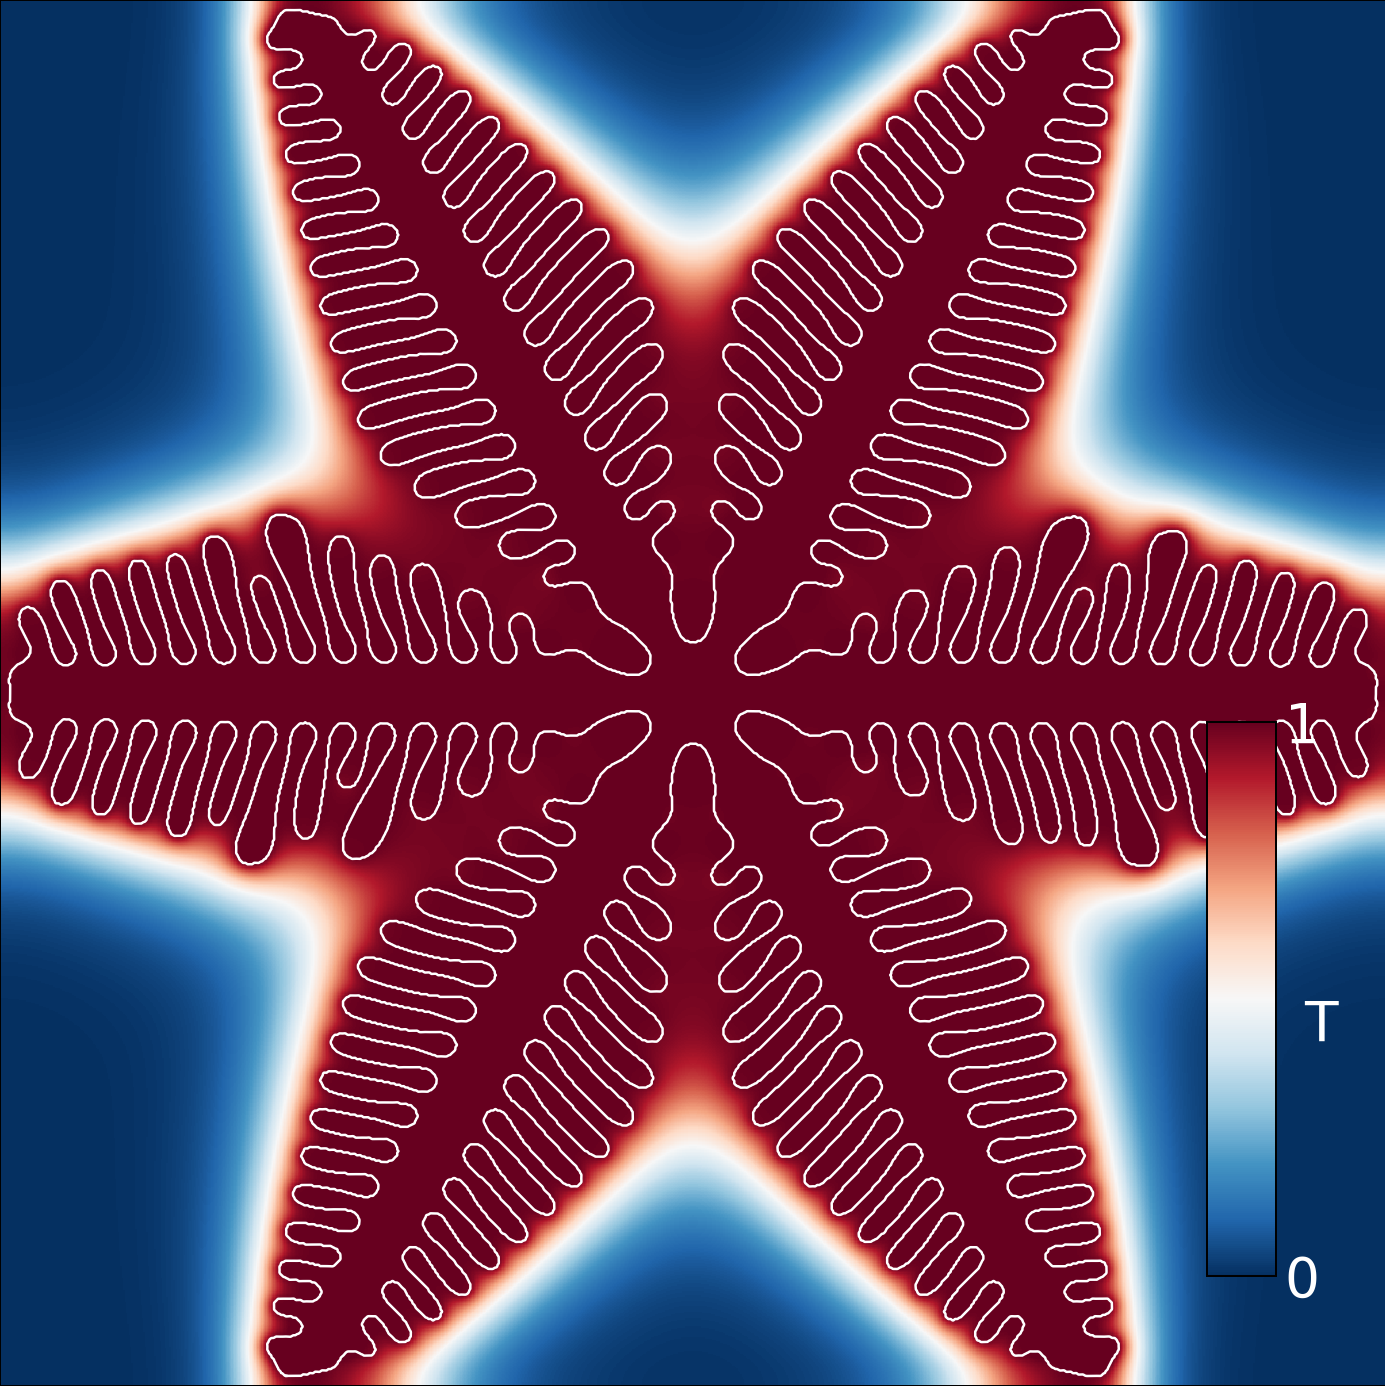
\includegraphics[width=\subfigwidth]{results/semi_long_neumann_FU_10.png}} &
    {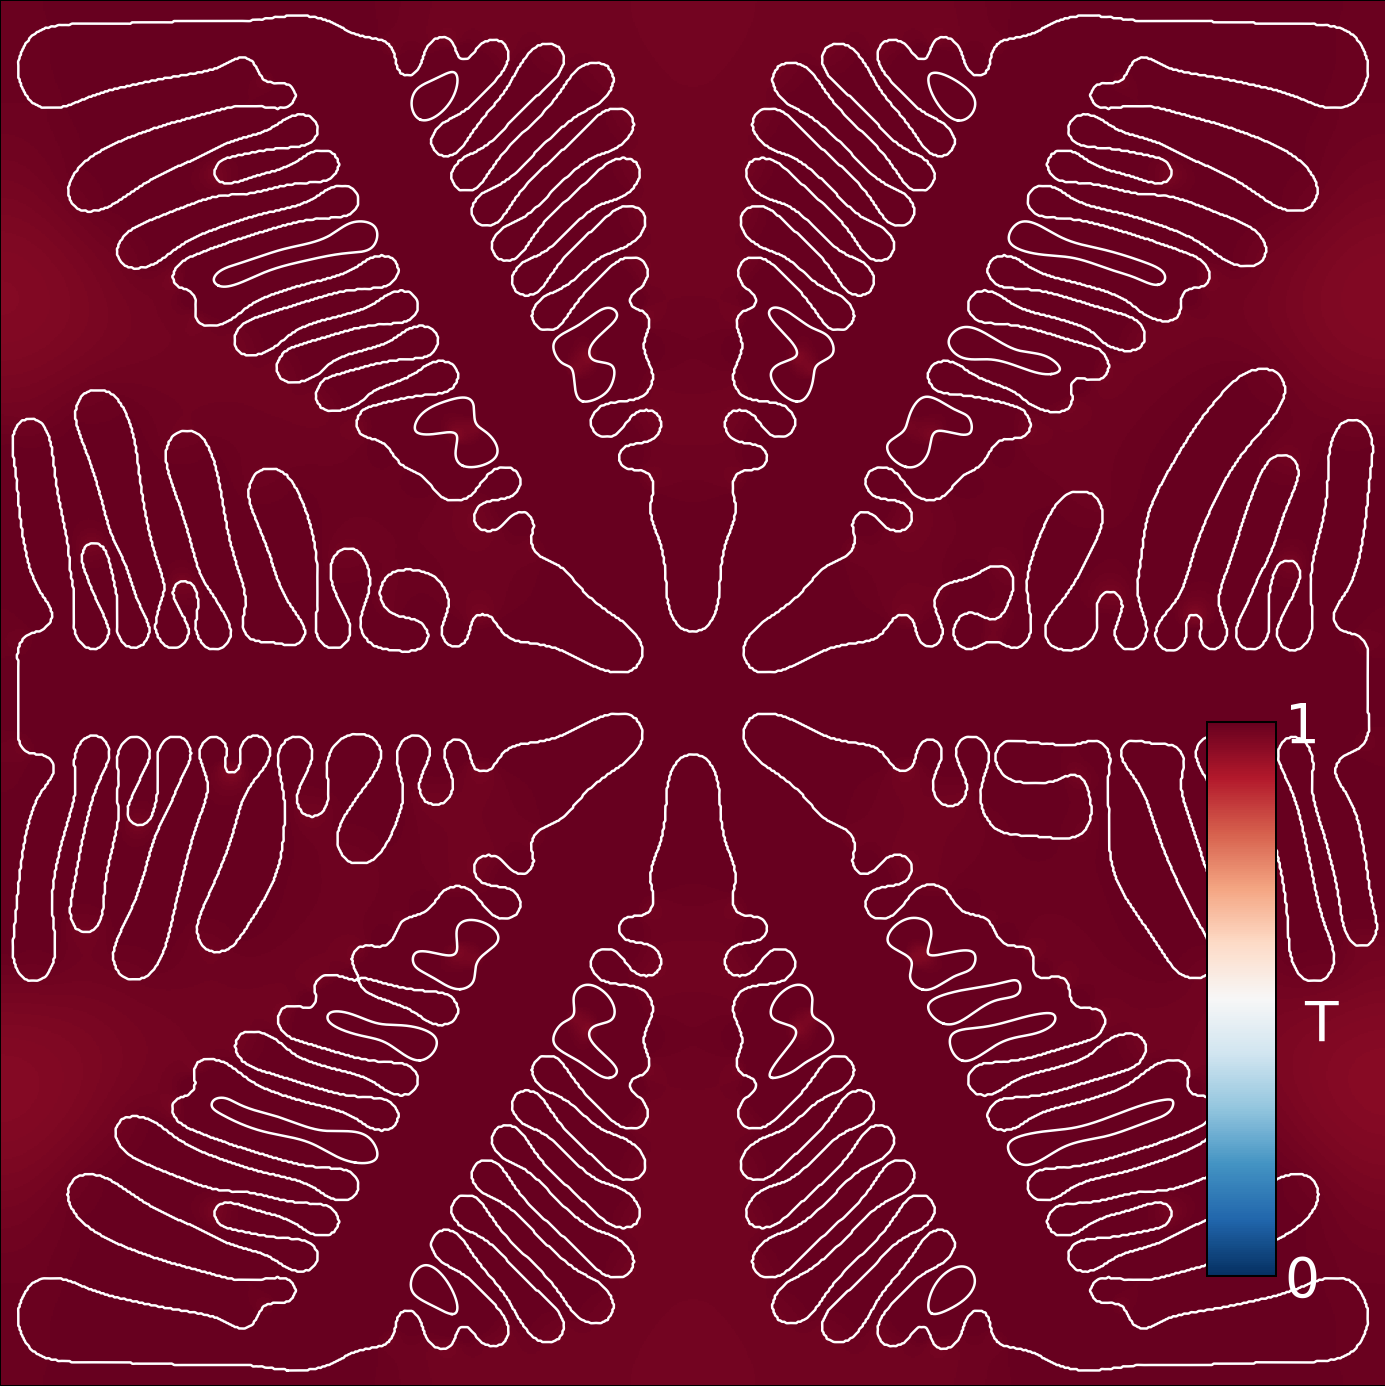
\includegraphics[width=\subfigwidth]{results/semi_long_neumann_FU_30.png}} &
    {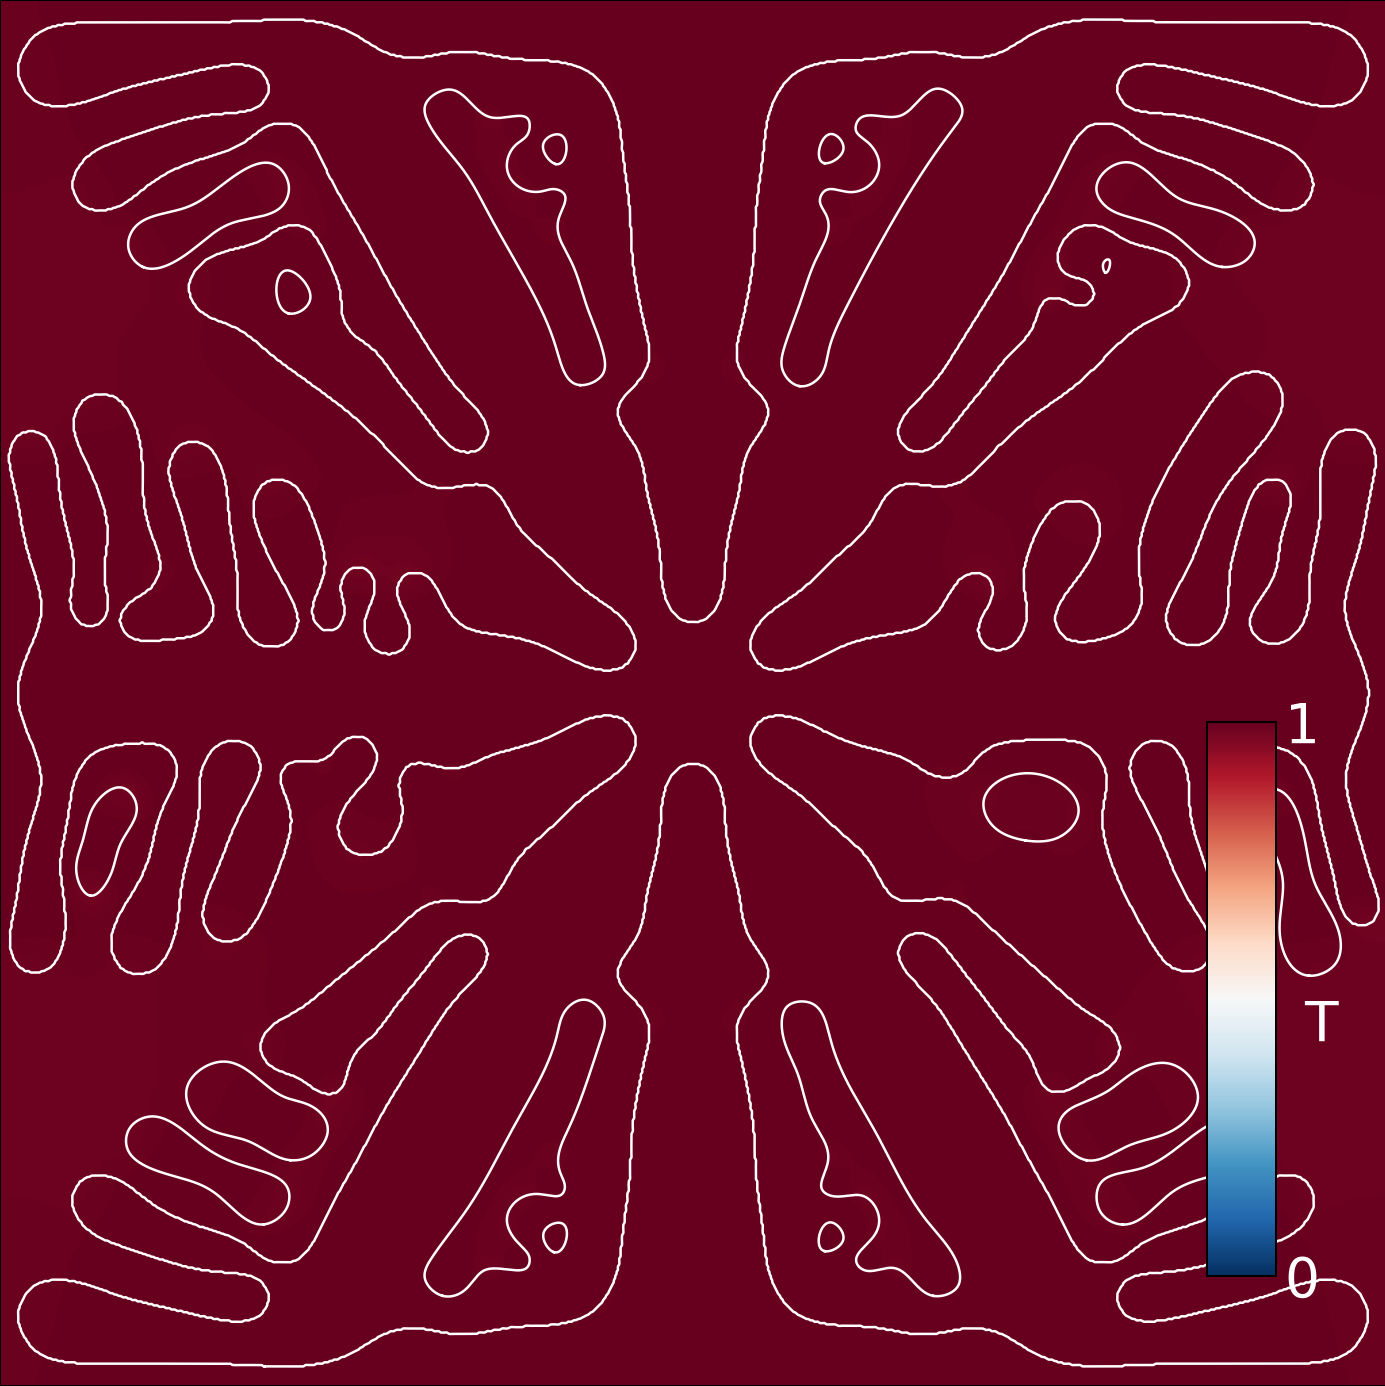
\includegraphics[width=\subfigwidth]{results/semi_long_neumann_FU_60.png}} \\
    $t = 0.1$ & 
    $t = 0.3$ &
    $t = 0.6$ 
    
    \end{tabular}
    \caption{
        Evolution of the temperature field and the phase interface $\Gamma$ (in white) over the time interval $\Timeint = [0, 0.6]$. Simulation setup given in Section \ref{sec:simulation setup} was used. The system reaches state of near thermodynamic equilibrium and coarsening of the crystal structure is observed (see Section \ref{sec:simulation boundary conditions}).
    }
    \label{fig:s-i filling}
\end{figure}
\FloatBarrier

\FloatBarrier
\begin{figure}[!ht]
    \centering
    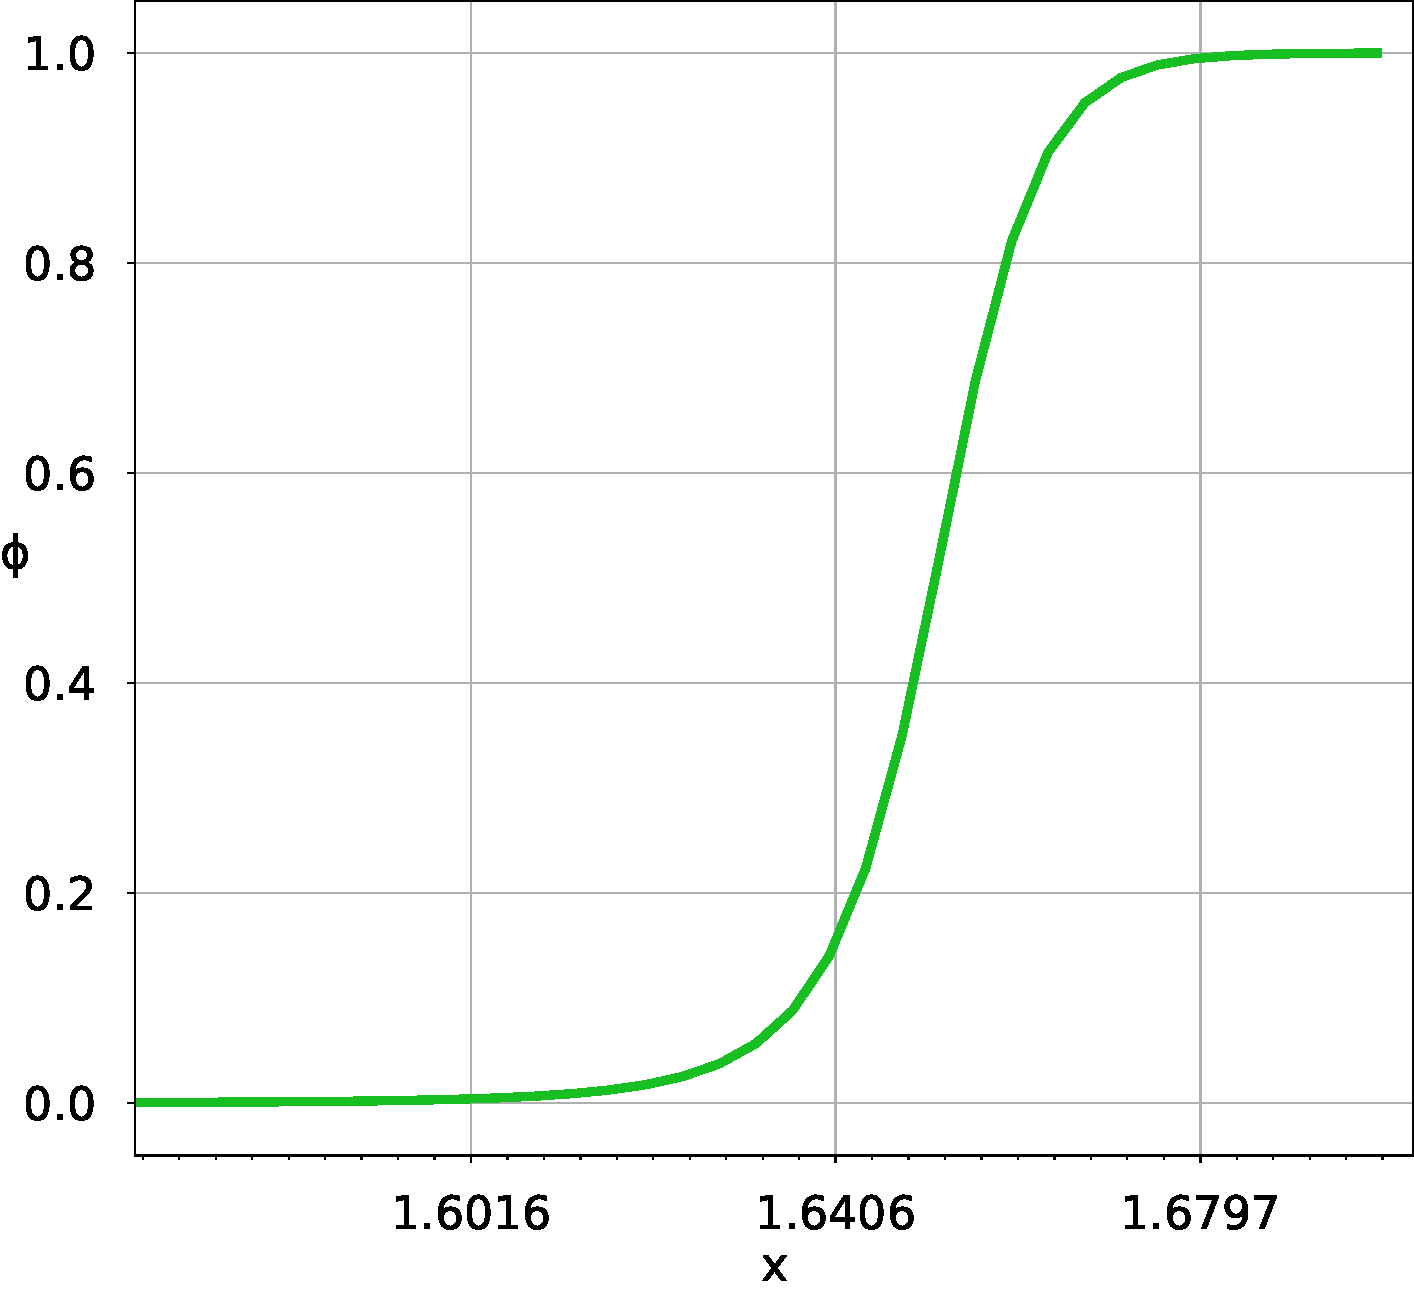
\includegraphics[height=8cm]{results/show_aniso_inteface_graph.pdf}
    \caption{Cross section of phase field at $y = 0$ showing the shape of the phase interface. Simulation setup given in Section \ref{sec:simulation setup} was used. Anisotropy strength $S$ was set to 0. Small ticks on the $x$ axis are $\dx$ apart. The phase interface is approximately $20\dx$ or $18\xi$ thick, where we consider the phase interface to be all values of $\Phi$ between $[0.01, 0.99]$. Similar values of $\xi$ have been observed in \cite{Strachota_dendric_crystal}.
    }
    \label{fig:phase interface result}
\end{figure}
\FloatBarrier

\section{Model comparison}
We verify the consistency of the proposed numerical methods by cross-comparison. We show results of the semi-implcit and various explicit schemes and extensively quantify the difference between these results.

% \iffalse
% \subsection{Phase field difference metric}
% To asses similarity of the resulting crystal structures two metrics are used. Let $\vec{F}_1, \vec{F}_2 \in\R^N$ be vectors of the discretized phase fields $\Phi_1, \Phi_2$ respectively given by (\ref{def: vector state notation}) for some $N\in\Nats$. We define the \emph{phase field norm} (PFN) as
% \begin{align}
%     PFN(\vec{F}_1) = \dx\dy\norm{\vec{F}_1}_1 \label{eq: phase field distance},
% \end{align} 
% the \emph{phase field distance} (PFD) as 
% \begin{align}
%     PFD(\vec{F}_1, \vec{F}_2) = \dx\dy\norm{\vec{F}_1 - \vec{F}_2}_1 \label{eq: phase field distance}
% \end{align} 
% and the \emph{phase field discrete distance} (PFDD) as 
% \begin{align}
%     PFDD(\vec{F}_1, \vec{F}_2) = \dx\dy\norm{D(\vec{F}_1) - D(\vec{F}_2)}_1, \label{eq: phase field discrete distance}
% \end{align} 
% where $D(\vec{F})$ is a function that evaluates to vector representing whether cells are considered solid, that is
% \begin{align}
%     D(\vec{F})_i = \begin{cases}
%         1, & \text{ when } F_i \ge \frac{1}{2} \\
%         0  & \text{ otherwise }
%     \end{cases} && \forall i \in \hat{N}.
% \end{align} 

% The phase field discrete distance (PFDD) (\ref{eq: phase field discrete distance}) represent the volume of the symmetric set difference of the two regions occupied by the solid phase. That is
% \newcommand{\setbar}[0]{\text{ }\middle|\text{ }}
% \begin{align}
%     PFDD(\vec{F}_1, \vec{F}_2)
%         &= m\left(\left\{\vec{x} \in C \setbar \Phi_{1,C} \ge \frac{1}{2}, C \in \Cells \right\} \bigtriangleup \left\{\vec{x} \in C \setbar \Phi_{2,C} \ge \frac{1}{2}, C \in \Cells \right\}\right)
%         % & \approx m(\left\{\vec{x} \in \Domain \setbar \Phi_1(t, \vec{x}) \ge \frac{1}{2} \right\} \bigtriangleup \left\{\vec{x} \in \Domain \setbar \Phi_2(t, \vec{x}) \ge \frac{1}{2} \right\} ),
% \end{align} where $t \in \Timeint$ and $\bigtriangleup$ is the symmetric set difference defined for two sets $A, B$ as 
% \begin{align}
%     A \bigtriangleup B = (A \setminus B) \cup (B \setminus A).
% \end{align}

% However in certain cases, such as when comparing the value of the step residual $r_\Phi$, we are interested in small difference of the phase field better captured by the phase field distance (PFD) (\ref{eq: phase field distance}). Because of the continuous nature of the model, these small differences are enough to, for example, indicate where the crystal might branch off in the future. 

% Note that in particular $L_\infty$ distance is a poor fit for the phase field as even small differences in the crystal position result in the maximum difference close to $1$.

% \fi

\subsection{Phase field difference metric}
To asses similarity of the resulting crystal structures, we will introduce two metrics. Let $\Phi_1, \Phi_2:\Timeint\times\Domain\to[0, 1]$ be phase fields as defined in Section \ref{sec:phase field model} and let $\Phi_{1,d}, \Phi_{2,d}:\Timeint \times \Cells \to [0, 1]$ be their corresponding mesh functions as described in Section \ref{sec:general mesh}. For the purpose of this section we are only interested in their values at some concrete time $t \in \Timeint$, so let $\Phi_{i} = \Phi_{i}(t, \cdot)$ and $\Phi_{i,d} = \Phi_{i,d}(t, \cdot)$, $i=1,2$. Lastly, we employ an additional discretization function $D:\R \to \{0, 1\}$ which is defined as
\begin{align}
    D(x) = \begin{cases}
        1, & \text{ when } x \ge \frac{1}{2} \\
        0  & \text{ otherwise }
    \end{cases} && \forall x \in \R.
\end{align}

We define the phase \emph{phase field norm} (PFN)
\begin{align}
    PFN(\Phi_1) &= \norm{\Phi_1}_{L_1(\Omega)} = \int_{\Omega} \abs{\Phi_1(\vec{x})} \dd \vec{x},
\end{align}
the \emph{phase field distance} (PFD) as 
\begin{align}
    PFD(\Phi_1, \Phi_2) = PFN(\Phi_1 - \Phi_2) \label{eq: phase field distance},
\end{align}
and the \emph{phase field discrete distance} (PFDD) as 
\begin{align}
    PFDD(\Phi_1, \Phi_2) = PFN(D \circ \Phi_1 - D \circ \Phi_2) \label{eq: phase field discrete distance}.
\end{align}
The phase field discrete distance (PFDD) (\ref{eq: phase field discrete distance}) represents the volume of the symmetric set difference of the two regions occupied by the solid phase. That is

\newcommand{\setbar}[0]{\text{ }\middle|\text{ }}
\begin{align}
    PFDD(\Phi_1, \Phi_2)
        &= m\left(\left\{\vec{x} \in \Omega \setbar \Phi_1(x) \ge \frac{1}{2} \right\} \bigtriangleup \left\{\vec{x} \in \Omega \setbar \Phi_2(x) \ge \frac{1}{2} \right\}\right),
\end{align} where $m$ is the Lebesgue measure and $\bigtriangleup$ is the symmetric set difference defined for two sets $A, B$ as 
\begin{align}
    A \bigtriangleup B = (A \setminus B) \cup (B \setminus A).
\end{align}

However in certain cases, such as when comparing the value of the step residual $r_\Phi$, we are interested in small difference of the phase field better captured by the phase field distance (PFD) (\ref{eq: phase field distance}). Because of the continuous nature of the model, these small differences are enough to, for example, indicate where the crystal might branch off in the future. 
Note that in particular $L_\infty$ distance is an inconvenient tool for assessing the differences for the phase field as even small differences in the crystal position result in the maximum difference close to $1$.

To extend the above definitions for the mesh functions $\Phi_{1,d}, \Phi_{2,d}$ we introduce the piecewise constant interpolation function
\begin{align}
    I:\Domain \to \Cells: \vec{x} \mapsto C \in \Cells \text{ such that } \vec{x} \in C,
\end{align}
and use it to define 
\begin{align}
    PFN(\Phi_d) &= PFN(\Phi_d \circ I), \\
    PFD(\Phi_{1,d}, \Phi_{2,d}) &= PFD(\Phi_{1,d} \circ I, \Phi_{2,d} \circ I), \\
    PFDD(\Phi_{1,d}, \Phi_{2,d}) &= PFDD(\Phi_{1,d} \circ I, \Phi_{2,d} \circ I).
\end{align}

\noindent
Specifically for uniform rectangular mesh, we can compute PFDD as
\begin{align}
    % PFDD(\vec{F}_1, \vec{F}_2) 
    PFDD(\Phi_{1,d}, \Phi_{2,d})
    = \dx\dy\norm{D(\vec{F}_1) - D(\vec{F}_2)}_1,
\end{align} 
where $\vec{F}_1, \vec{F}_2 \in\R^N$ are vectors of the mesh functions $\Phi_{1,d}, \Phi_{2,d}$, respectively, given by (\ref{def: vector state notation}) and function $D$ is applied element-wise. PFN and PFD can be computed similarly.

\FloatBarrier
\begin{figure}[!ht]
    \centering
    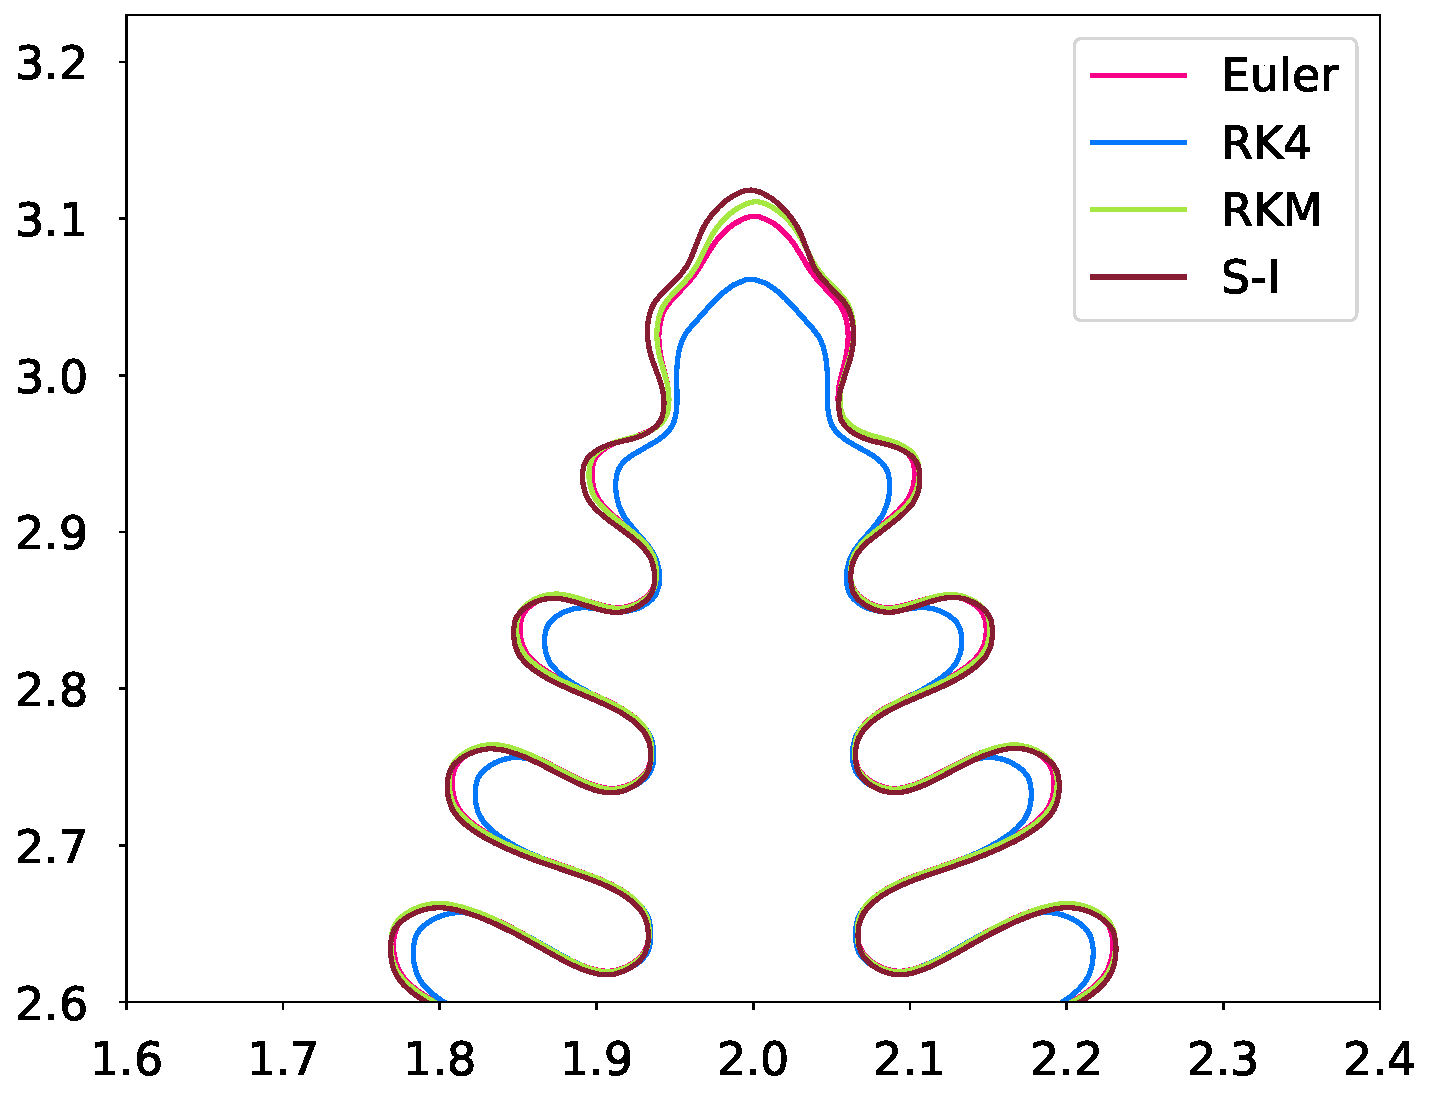
\includegraphics[height=8cm]{results/model_comp.pdf}
    \caption{
        Comparison of crystal structures for different numerical schemes at $t = 0.04$. Simulation setup given in Section \ref{sec:simulation setup} was used with changed $\dt = 2.5\times10^{-5}$. The phase interface obtained using the Euler, RK4, RKM and S-I schemes is shown.
    }
    \label{fig:model comp}
\end{figure}
\FloatBarrier

\FloatBarrier
\begin{table}[!ht]
\centering
\begin{tabular}{|l|r|r|r|r|}
    \hline
    & & & & \\[-1em]
    Schemes  & \multicolumn{1}{c|}{Euler} & \multicolumn{1}{c|}{RK4} & \multicolumn{1}{c|}{RKM} & \multicolumn{1}{c|}{S-I} \\
    \hline
    & & & & \\[-1em]
    Euler   & $0$ & $9.02\times 10^{-2}$ & $1.52\times 10^{-2}$ & $5.36\times 10^{-2}$ \\
    \hline
    & & & & \\[-1em]
    RK4     & $9.02\times 10^{-2}$ & $0$ & $1.01\times 10^{-1}$ & $1.24\times 10^{-1}$ \\
    \hline
    & & & & \\[-1em]
    RKM     & $1.52\times 10^{-2}$ & $1.01\times 10^{-1}$ & $0$ & $4.43\times 10^{-2}$ \\
    \hline
    & & & & \\[-1em]
    S-I     & $5.36\times 10^{-2}$ & $1.24\times 10^{-1}$ & $4.43\times 10^{-2}$ & $0$ \\
    \hline 
\end{tabular}

    \caption{Phase field discrete distance (PFDD) between results obtained by different integration schemes. Refer to Figure \ref{fig:model comp} for the experiment setup.}
    \label{table:scheme comparison vdist}
\end{table}
\FloatBarrier

\FloatBarrier
\begin{table}[!ht]
\centering
\begin{tabular}{|l|r|r|r|r|}
    \hline
    & & & & \\[-1em]
    Schemes  & \multicolumn{1}{c|}{Euler} & \multicolumn{1}{c|}{RK4} & \multicolumn{1}{c|}{RKM} & \multicolumn{1}{c|}{S-I} \\
    \hline
    & & & & \\[-1em]
    Euler   & $0$ & $9.05\times 10^{-2}$ & $1.49\times 10^{-2}$ & $5.20\times 10^{-2}$ \\
    \hline
    & & & & \\[-1em]
    RK4     & $9.05\times 10^{-2}$ & $0$ & $1.01\times 10^{-1}$ & $1.23\times 10^{-1}$ \\
    \hline
    & & & & \\[-1em]
    RKM     & $1.49\times 10^{-2}$ & $1.01\times 10^{-1}$ & $0$ & $4.32\times 10^{-2}$ \\
    \hline
    & & & & \\[-1em]
    S-I     & $5.20\times 10^{-2}$ & $1.23\times 10^{-1}$ & $4.32\times 10^{-2}$ & $0$ \\
    \hline 
\end{tabular}

    \caption{Phase field distance (PFD) between results obtained by different integration schemes. Refer to Figure \ref{fig:model comp} for the experiment setup.}
    \label{table:scheme comparison edist}
\end{table}
\FloatBarrier


From Figure \ref{fig:model comp} and Tables \ref{table:scheme comparison edist}, \ref{table:scheme comparison vdist}, we conclude that the proposed schemes produce similar crystal structure, with the RK scheme differing most significantly. Because of this, it will not be included in further discussions. Furthermore, the values obtained from phase field distance (PFD) and phase field discrete distance (PFDD) are almost identical. This is caused by the phase field function, which is, apart from the thin phase interface, very close to either $0$ or $1$. As such we will only list the PFDD distance in scheme comparison from now on.

\section{Correction impact}
We explore the effect of the proposed solutions to reduce the error introduced by operator splitting, namely repeated time stepping and correction term (see Sections \ref{sec:repeated time stepping} and \ref{sec:correction term}). 

Even though repeated time stepping is applicable to all proposed numerical schemes, it has only been developed for the the S-I and Euler schemes, which will be used in the presented results. The correction term modification is presented for the S-I, RKM and Euler schemes.


\FloatBarrier
\begin{figure}[!ht]
    \centering
    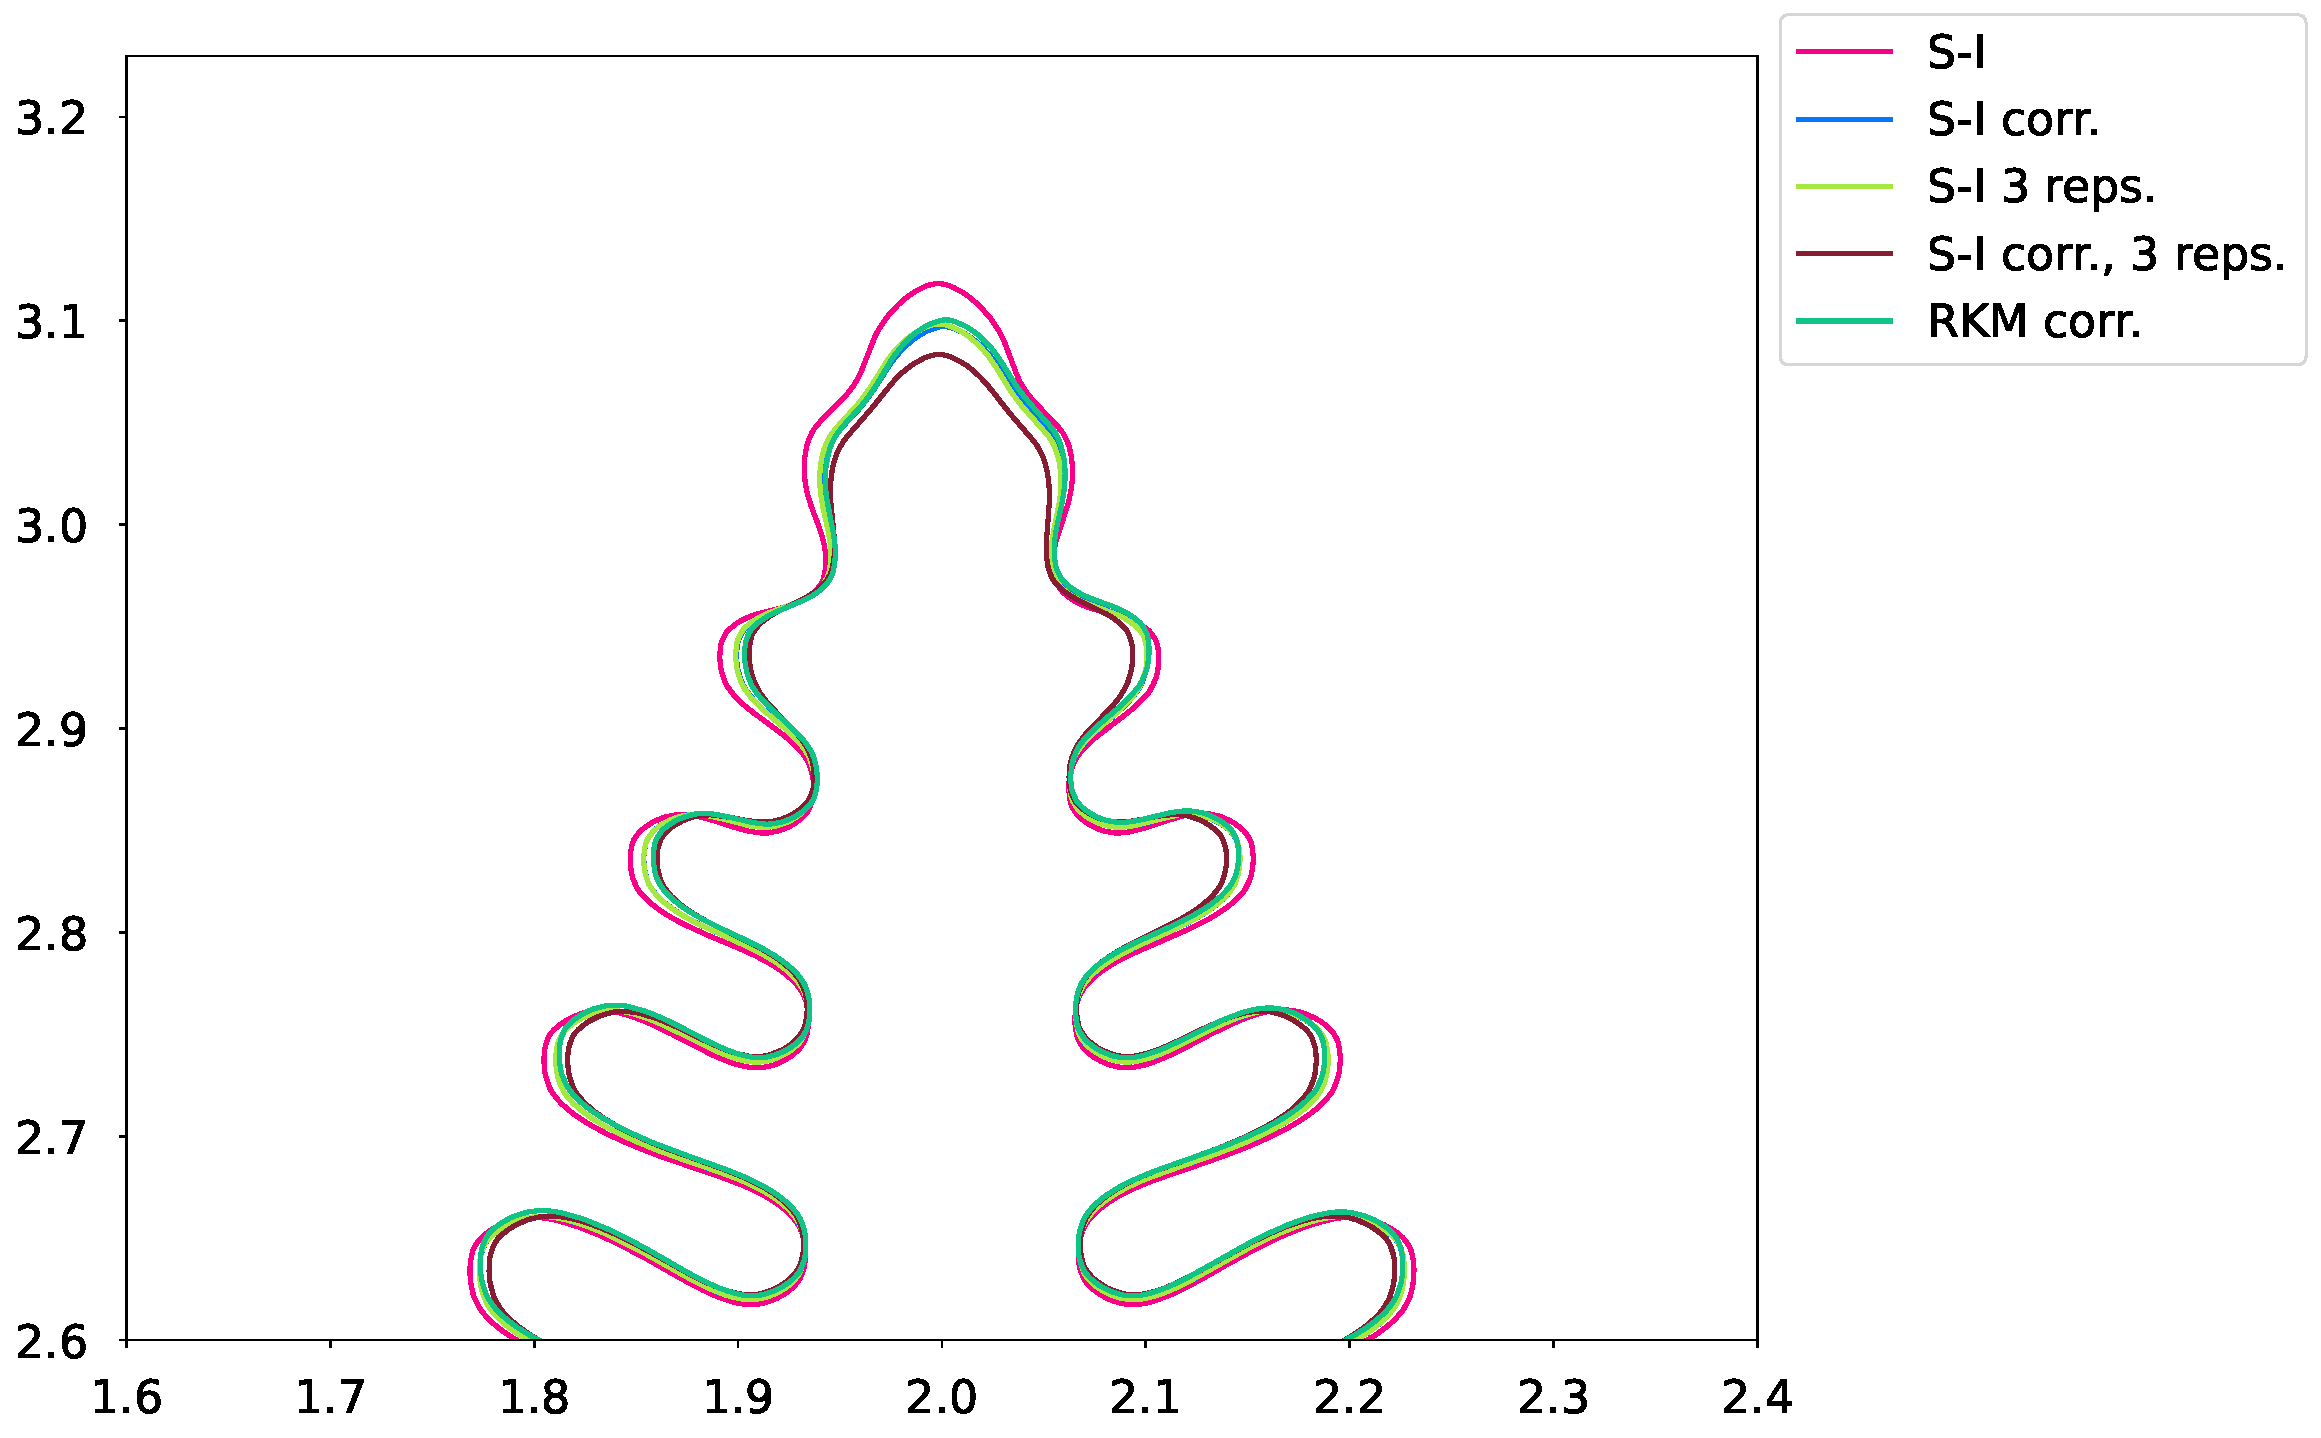
\includegraphics[height=8cm]{results/correction_comp.pdf}
    \caption{
        Comparison of crystal structures for different numerical schemes with repeated time stepping and correction term modifications at $t = 0.04$. Simulation setup given in Section~\ref{sec:simulation setup} was used except for the setting $\dt = 2.5\times10^{-5}$. Schemes marked with the abbreviation "corr." use the correction term modification, described in Section~\ref{sec:correction term}. Schemes marked with the abbreviation "3 reps." use repeated time stepping, described in Section~\ref{sec:repeated time stepping}, with $M = 3$, $\varepsilon = 0$, $\alpha = 1$ (see Algorithm~\ref{alg:fractional timestepping}).
    }
    \label{fig:correction comp}
\end{figure}
\FloatBarrier

As shown in Figure \ref{fig:correction comp}, the crystal structure is very similar for all modifications. Operator splitting corrections make the crystal grow "slower", so the majority of the error is found at the tips of a dendrites where the crystal grows the fastest. When used separately, repeated time stepping and correction term modification both achieve remarkably similar results for the S-I scheme (see Table \ref{table:correction comp vdist}). When used in conjunction, they seem to produce different structures compared to the rest of the schemes. 

\setlength{\subfigwidth}{0.48\textwidth}
\FloatBarrier
\begin{figure}[!ht]
    \centering
    \begin{subfigure}[t]{\subfigwidth}
        \centering
        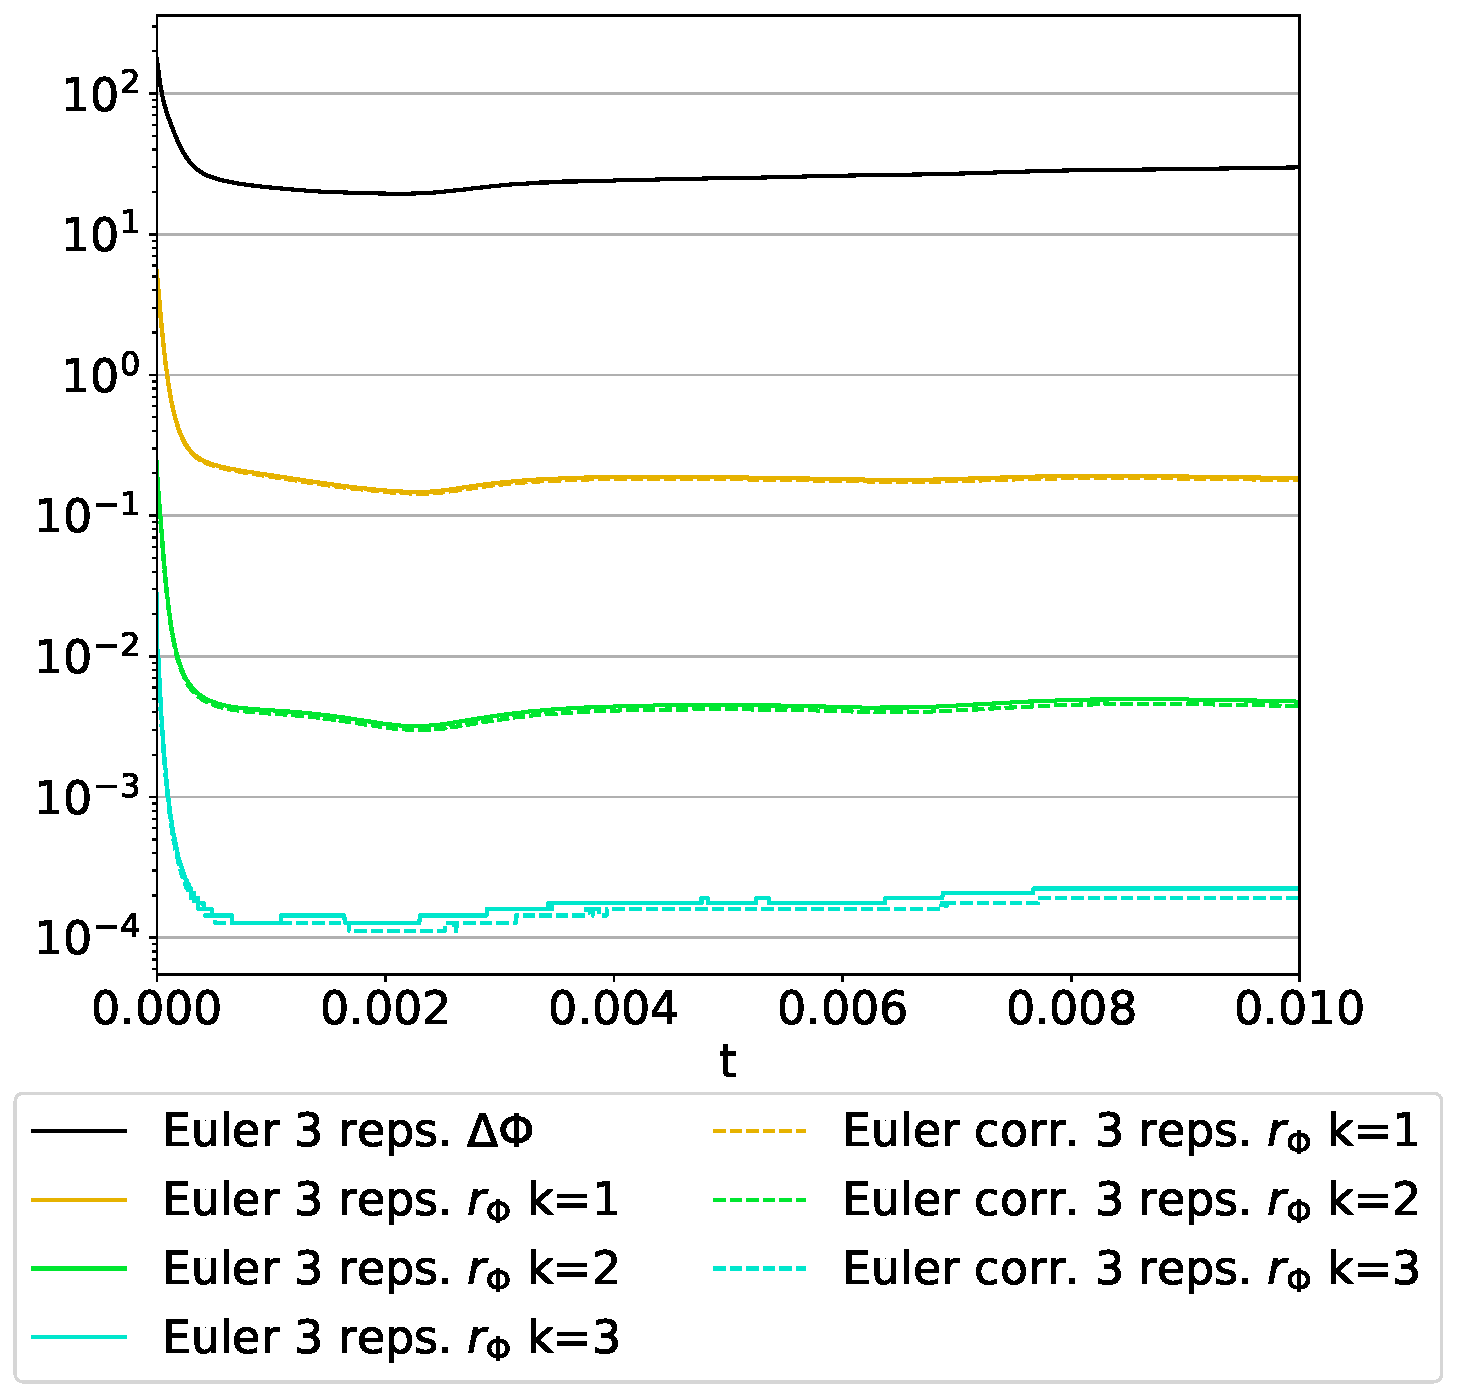
\includegraphics[height=7cm]{results/step_res_comp_euler.pdf}
        \caption{Explicit scheme using Euler method}
        \label{fig:step res comp euler}
    \end{subfigure}
    \begin{subfigure}[t]{\subfigwidth}
        \centering
        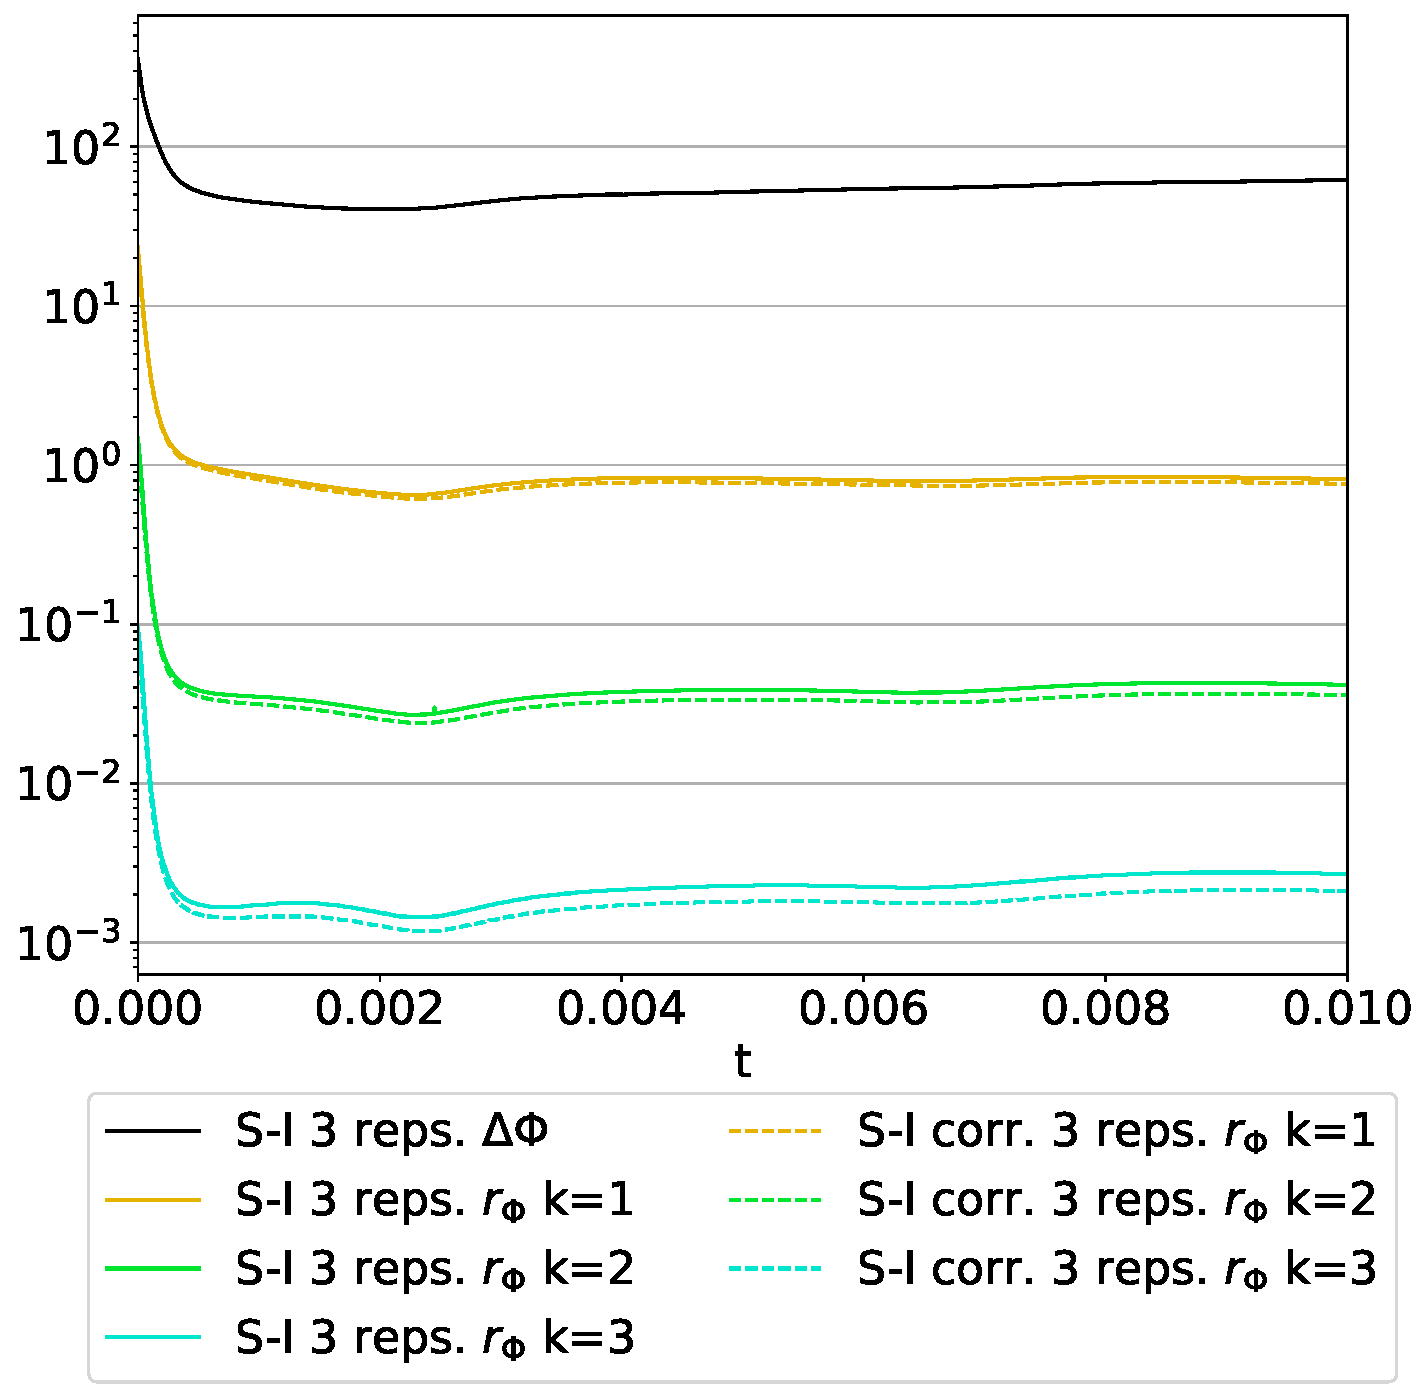
\includegraphics[height=7cm]{results/step_res_comp_semi.pdf}
        \caption{Semi-Implicit scheme}
        \label{fig:step res comp semi}
    \end{subfigure}
    
    \caption{
        Evolution of the phase field norm (PFN) of the $n$-th step residual $\vec{r}_\Phi$ for the Euler and S-I schemes. $\Delta \Phi$ is the phase field distance (PFD) between the current and next time step, that is $\Delta \Phi = PFD(\vec{F}^{n+1}, \vec{F}^{n})$, where $\vec{F}^n$ represents discretized phase field $\Phi$ is in the timestep $n$ given by (\ref{def: vector state notation}). 
        $r_\Phi \text{ \#}k$, $k \in \{1,2,3\}$ marks the value of $PFN(r_\Phi)$ in the $k$-th iteration of Algorithm~\ref{alg:fractional timestepping}.
        Schemes marked with the abbreviation "corr." use the correction term modification, described in Section~\ref{sec:correction term}. Schemes marked with the abbreviation "3 reps." use repeated time stepping, described in Section~\ref{sec:repeated time stepping}, with $M = 3$, $\varepsilon = 0$, $\alpha = 1$.
        Simulation setup given in Section~\ref{sec:simulation setup} was used with changed $\dt = 2.5\times10^{-5}$ for the S-I scheme and $\dt = 1.2\times10^{-5}$ for the Euler scheme.
        High values near the start of the simulation are caused by the mismatch between the initial conditions given in Section \ref{sec:setup initial conditions} and the stable shape of the phase interface depicted in Figure \ref{fig:phase interface result}. Discrete jumps in values close to $10^{-4}$ are caused by the inability of the used storage format to represent small numbers.
    }
    \label{fig:step res comp}
\end{figure}
\FloatBarrier

From Figure \ref{fig:step res comp} we conclude that Algorithm \ref{alg:fractional timestepping} reduces the magnitude of the step residual $PFN(\vec{r}_\Phi)$ by more than an order of magnitude per iteration. On the other hand, the corrected schemes proposed in Section \ref{sec:correction term} have negligible impact on the value of $PFN(\vec{r}_\Phi)$. Similar trends are observed for $\vec{r}_\Phi$ in the $L_2$ and $L_\infty$ norms.



% \begin{table}[!ht]
% \centering
% \begin{tabular}{|l|r|r|r|r|r|}
%     \hline
%     & & & & & \\[-1em]
%     Schemes  & \multicolumn{1}{c|}{S-I} & \multicolumn{1}{c|}{S-I corr.} & \multicolumn{1}{c|}{S-I 3 reps.} & \multicolumn{1}{c|}{S-I corr., 3 reps.} & \multicolumn{1}{c|}{RKM corr.} \\
%     \hline
%     & & & & & \\[-1em]
%     S-I     & $0$ & $5.54\times 10^{-2}$ & $5.53\times 10^{-2}$ & $1.07\times 10^{-1}$ & $9.07\times 10^{-2}$ \\
%     \hline
%     & & & & & \\[-1em]
%     S-I corr. & $5.54\times 10^{-2}$ & $0$ & $1.47\times 10^{-3}$ & $5.16\times 10^{-2}$ & $4.02\times 10^{-2}$ \\
%     \hline
%     & & & & & \\[-1em]
%     S-I 3 reps. & $5.53\times 10^{-2}$ & $1.47\times 10^{-3}$ & $0$ & $5.17\times 10^{-2}$ & $4.05\times 10^{-2}$ \\
%     \hline
%     & & & & & \\[-1em]
%     S-I corr., 3 reps. & $1.07\times 10^{-1}$ & $5.16\times 10^{-2}$ & $5.17\times 10^{-2}$ & $0$ & $3.30\times 10^{-2}$ \\
%     \hline
%     & & & & & \\[-1em]
%     RKM corr. & $9.07\times 10^{-2}$ & $4.02\times 10^{-2}$ & $4.05\times 10^{-2}$ & $3.30\times 10^{-2}$ & $0$ \\
%     \hline 
    
% \end{tabular}
%     \caption{Phase field distance (PFD) between different integration schemes using operator splitting corrections. Refer to Figure \ref{fig:correction comp} for the experiment setup. Note that the distance between the schemes employing correction term modification (S-I corr.) and repeated time stepping (S-I 3 reps.) is about an order of magnitude less then between any two other schemes. }
%     \label{table:correction comp edist}
% \end{table}

\begin{table}[!ht]
\centering
\begin{tabular}{|l|r|r|r|r|r|}
    \hline
    & & & & & \\[-1em]
    Schemes  & \multicolumn{1}{c|}{S-I} & \multicolumn{1}{c|}{S-I corr.} & \multicolumn{1}{c|}{S-I 3 reps.} & \multicolumn{1}{c|}{S-I corr., 3 reps.} & \multicolumn{1}{c|}{RKM corr.} \\
    \hline
    & & & & & \\[-1em]
    S-I     & $0$ & $5.52\times 10^{-2}$ & $5.52\times 10^{-2}$ & $1.05\times 10^{-1}$ & $9.14\times 10^{-2}$ \\
    \hline
    & & & & & \\[-1em]
    S-I corr. & $5.52\times 10^{-2}$ & $0$ & $1.56\times 10^{-3}$ & $5.06\times 10^{-2}$ & $4.01\times 10^{-2}$ \\
    \hline
    & & & & & \\[-1em]
    S-I 3 reps. & $5.52\times 10^{-2}$ & $1.56\times 10^{-3}$ & $0$ & $5.06\times 10^{-2}$ & $4.02\times 10^{-2}$ \\
    \hline
    & & & & & \\[-1em]
    S-I corr., 3 reps. & $1.05\times 10^{-1}$ & $5.06\times 10^{-2}$ & $5.06\times 10^{-2}$ & $0$ & $3.11\times 10^{-2}$ \\
    \hline
    & & & & & \\[-1em]
    RKM corr. & $9.14\times 10^{-2}$ & $4.01\times 10^{-2}$ & $4.02\times 10^{-2}$ & $3.11\times 10^{-2}$ & $0$ \\
    \hline 
    
\end{tabular}

    \caption{Phase field discrete distance (PFDD) between different integration schemes using operator splitting corrections. Refer to Figure \ref{fig:correction comp} for the experiment setup. Note that the distance between the schemes employing correction term modification (S-I corr.) and repeated time stepping (S-I 3 reps.) is about an order of magnitude smaller then between any two other schemes. }
    
    \label{table:correction comp vdist}
\end{table}
\FloatBarrier


\section{Computation time comparison}
Lastly, we compare the simulation running times to the reference parallel implementation in \cite{StrachotaDizertation}.

Since our implementation is limited to one GPU we do not attempt to determine strong or weak scaling. Instead we only compare the absolute running times on a fixed hardware. Artificially lowering the number of GPU threads available to our implementation is possible but is not practical and does not extrapolate to multi-GPU setups.

\vvskip
\FloatBarrier
\begin{table}[!ht]
    \centering
    % {
    % \setstretch{1.1}
    \begin{tabular}{ll} 
        \toprule
        $\Omega = (0, 4\cdot n/512)\times(0, 4 \cdot n/512)$ & $\Timeint = [0, 0.04]$ \\
        $n_x = n_y = n$ & $\dt = 5\times10^{-5}$ \\
        $\dx = \dy = 4/512$ & $\xi = 0.0043$ \\
        $a = 2$ & $\alpha = 3$ \\
        $b = 1$ & $\beta = 1400$ \\
        $L = 2$ & $T^* = 1$ \\
        $S = 0$ & $m = 6$ \\
        $\theta_0 = 0$ & \\
        \bottomrule
    \end{tabular}
    % }
    \caption{Benchmark model parameters}
    \label{tab:benchmark model parameters}
\end{table}
\FloatBarrier

The implementations were compared on simulation setup given in Table \ref{tab:benchmark model parameters} for values of $n \in \{128, 256, 512, 1024, 2048\}$. Homogeneous Neumnann boundary conditions were used for both temperature and phase
fields along with initial conditions from Section \ref{sec:setup initial conditions}. The anisotropy strength $S$ was set to 0 to be able to compare against the reference implementation (employing different model of anisotropy). The size of the computational domain $\Omega$ is scaled with $n$ causing $\dx, \dy$ to remain constant. This ensures the stability criterion for explicit schemes remains unchanged for all values of $n$. Similar parameters were used to obtain Figure \ref{fig:aniso param results} with $S = 0$. 

The implementation comparison was run on two different sets of hardware we will denote "consumer" and "HPC":
\begin{itemize}
    \item Consumer: NVIDIA GeForce MX450 w. 1.8GB RAM, 8-core 11th Gen Intel(R) Core(TM) i5-1135G7 @ 2.40GHz (SMT mode enabled), 16 GB RAM
    \item HPC: NVIDIA A100 SXM4 w. 80GB HBM2 RAM, 32-core AMD EPYC 7543 @ 2.8GHz CPU (SMT mode disabled), 1024 GB RAM
\end{itemize}
Consumer hardware is lower end of current available CUDA enabled GPUs while HPC is hardware for compute clusters well suited for scientific computation. Most other GPUs are expected to lie somewhere between these two. The HPC hardware was accessible on the faculty supercomputer HELIOS. 

The results are summarized in Figures \ref{fig:comp time broad comparison}, \ref{fig:comp time helios comparison}. Note that the reference implementation employs the RKM integration scheme, and thus only that scheme should be used for direct comparison.

\FloatBarrier
\begin{figure}[!ht]
    \centering
    \setlength{\subfigwidth}{0.48\textwidth}
    \setlength{\belowcaptionskip}{0.5\baselineskip}
    \begin{subfigure}[t]{\subfigwidth}
        \centering
        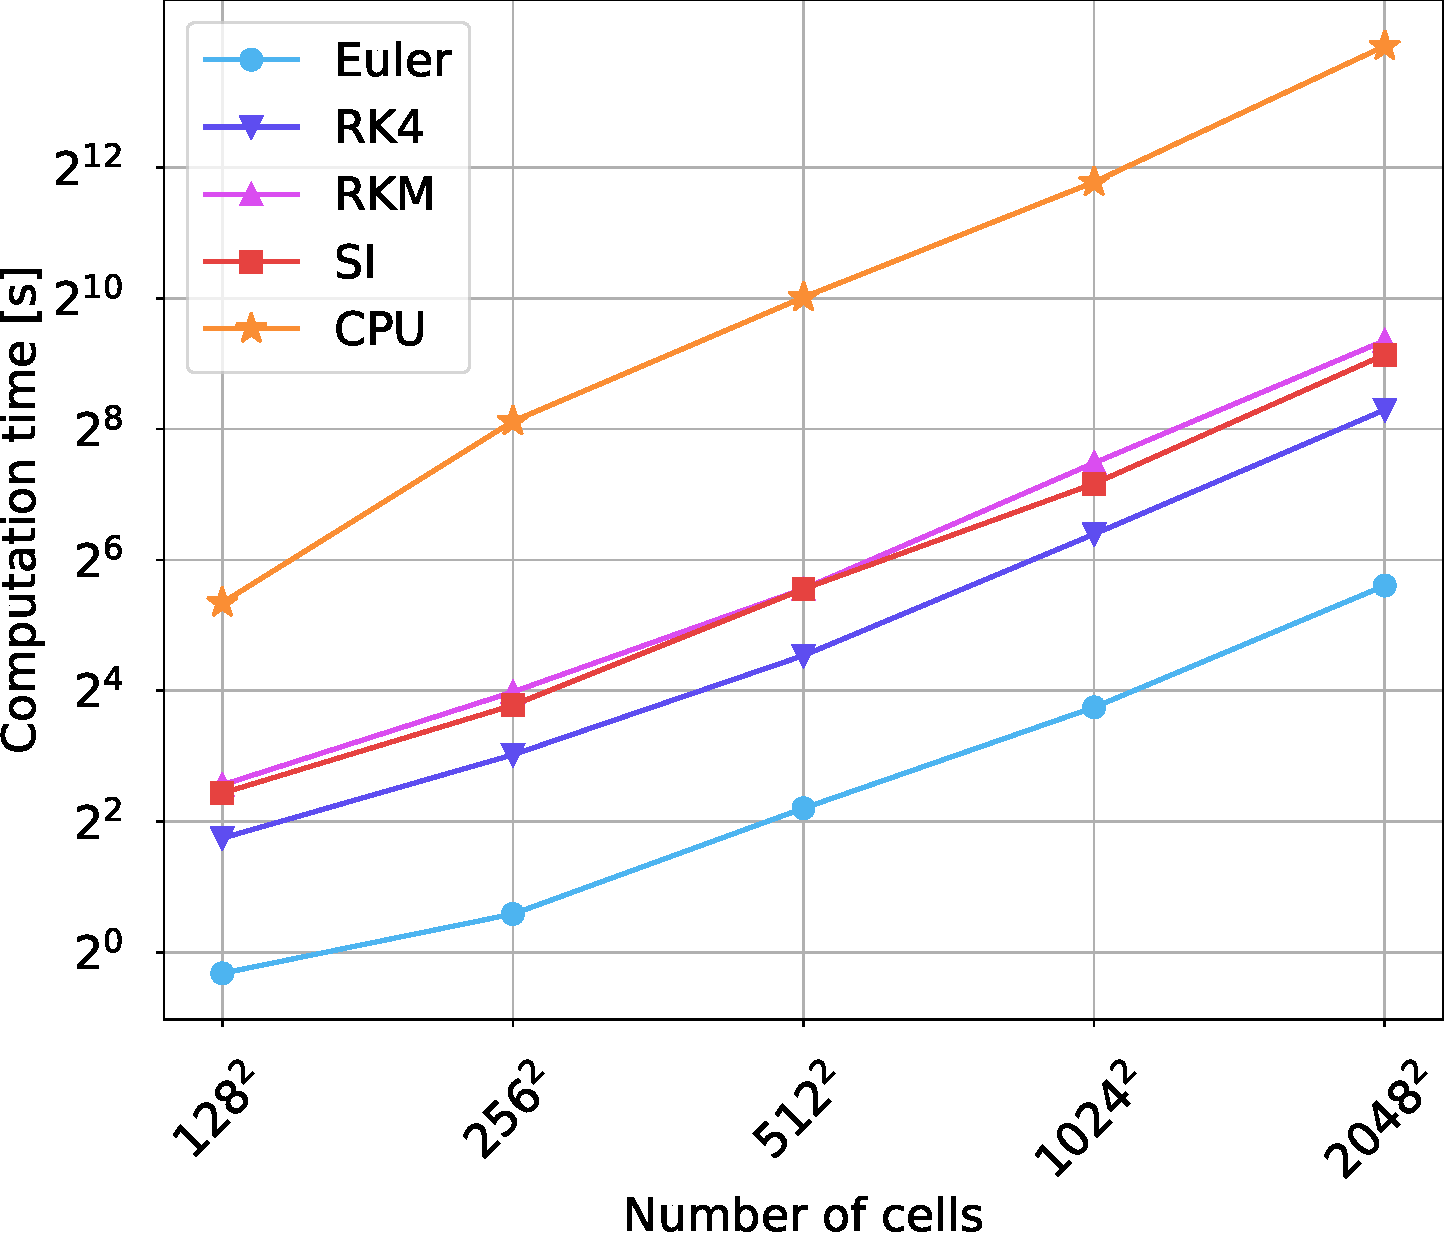
\includegraphics[width=0.95\textwidth]{results/comp_time_consumer.pdf}
        \caption{Computation time}
        \label{fig:comp time broad comparison}
    \end{subfigure}
    \hfill    
    \begin{subfigure}[t]{\subfigwidth}
        \centering
        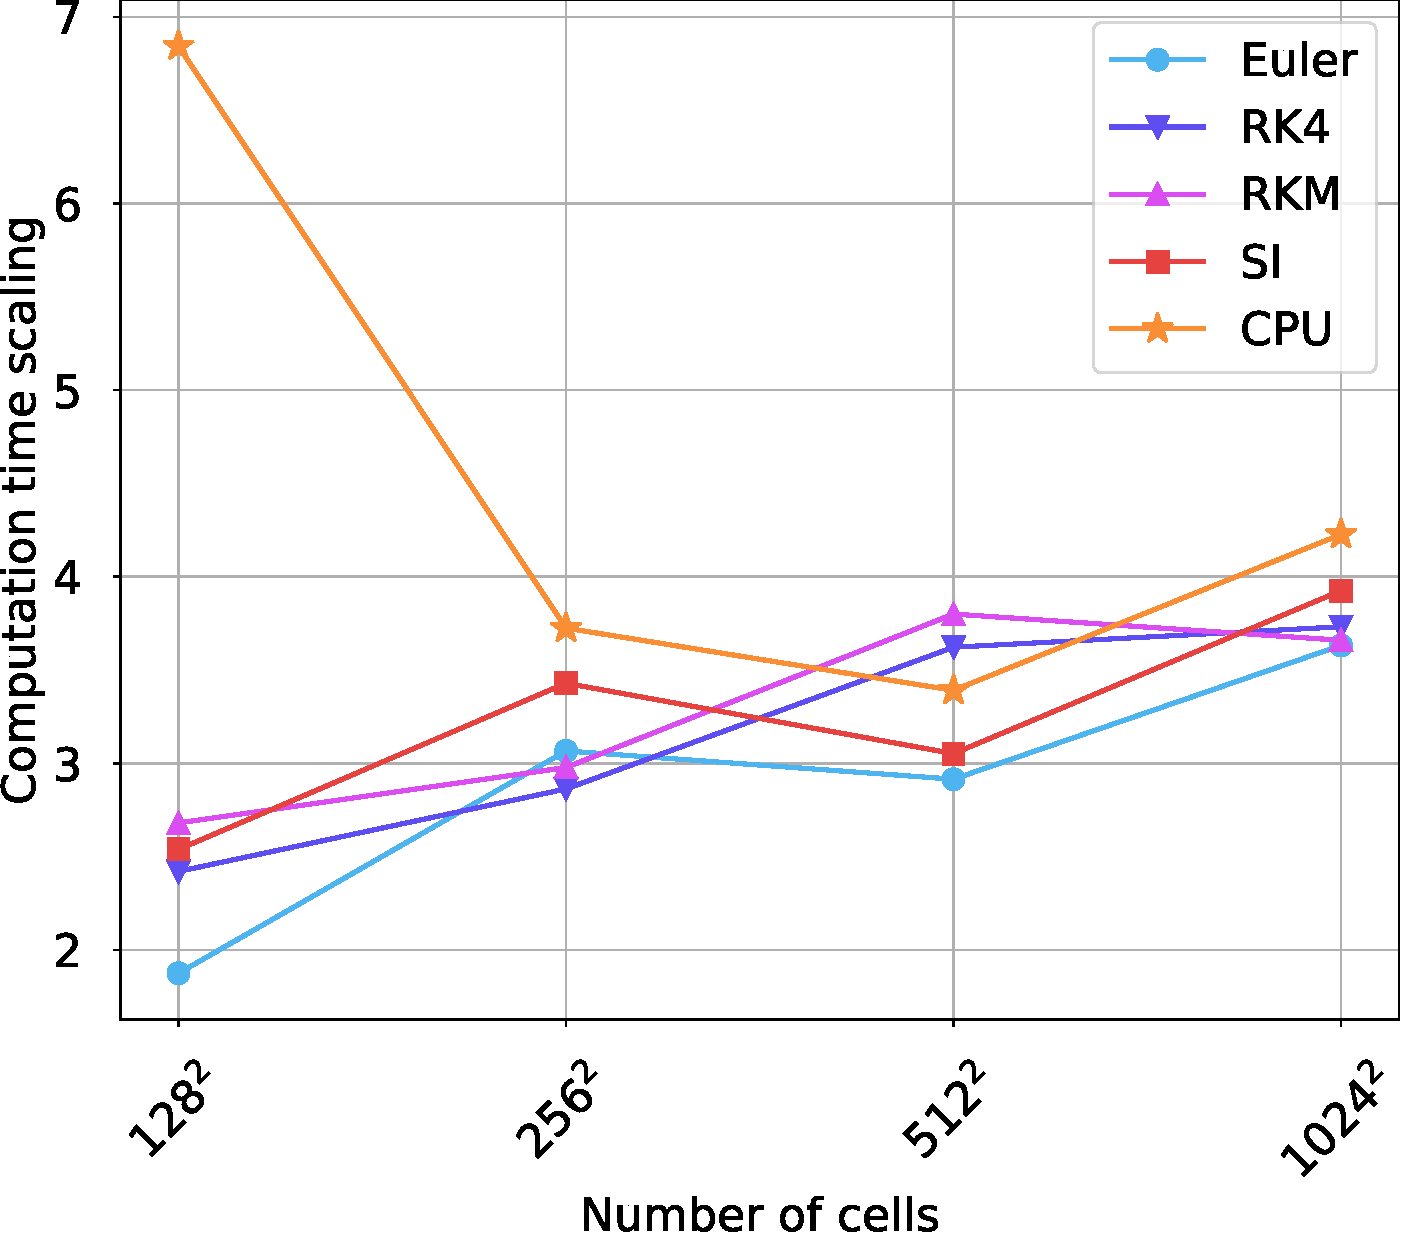
\includegraphics[width=0.95\textwidth]{results/comp_time_consumer_scaling.pdf}
        \caption{Computation time scaling}
        \label{fig:comp time broad comparison scaling}
    \end{subfigure}

    \par\vvskip
    \begin{subfigure}[t]{\textwidth}
        \centering
        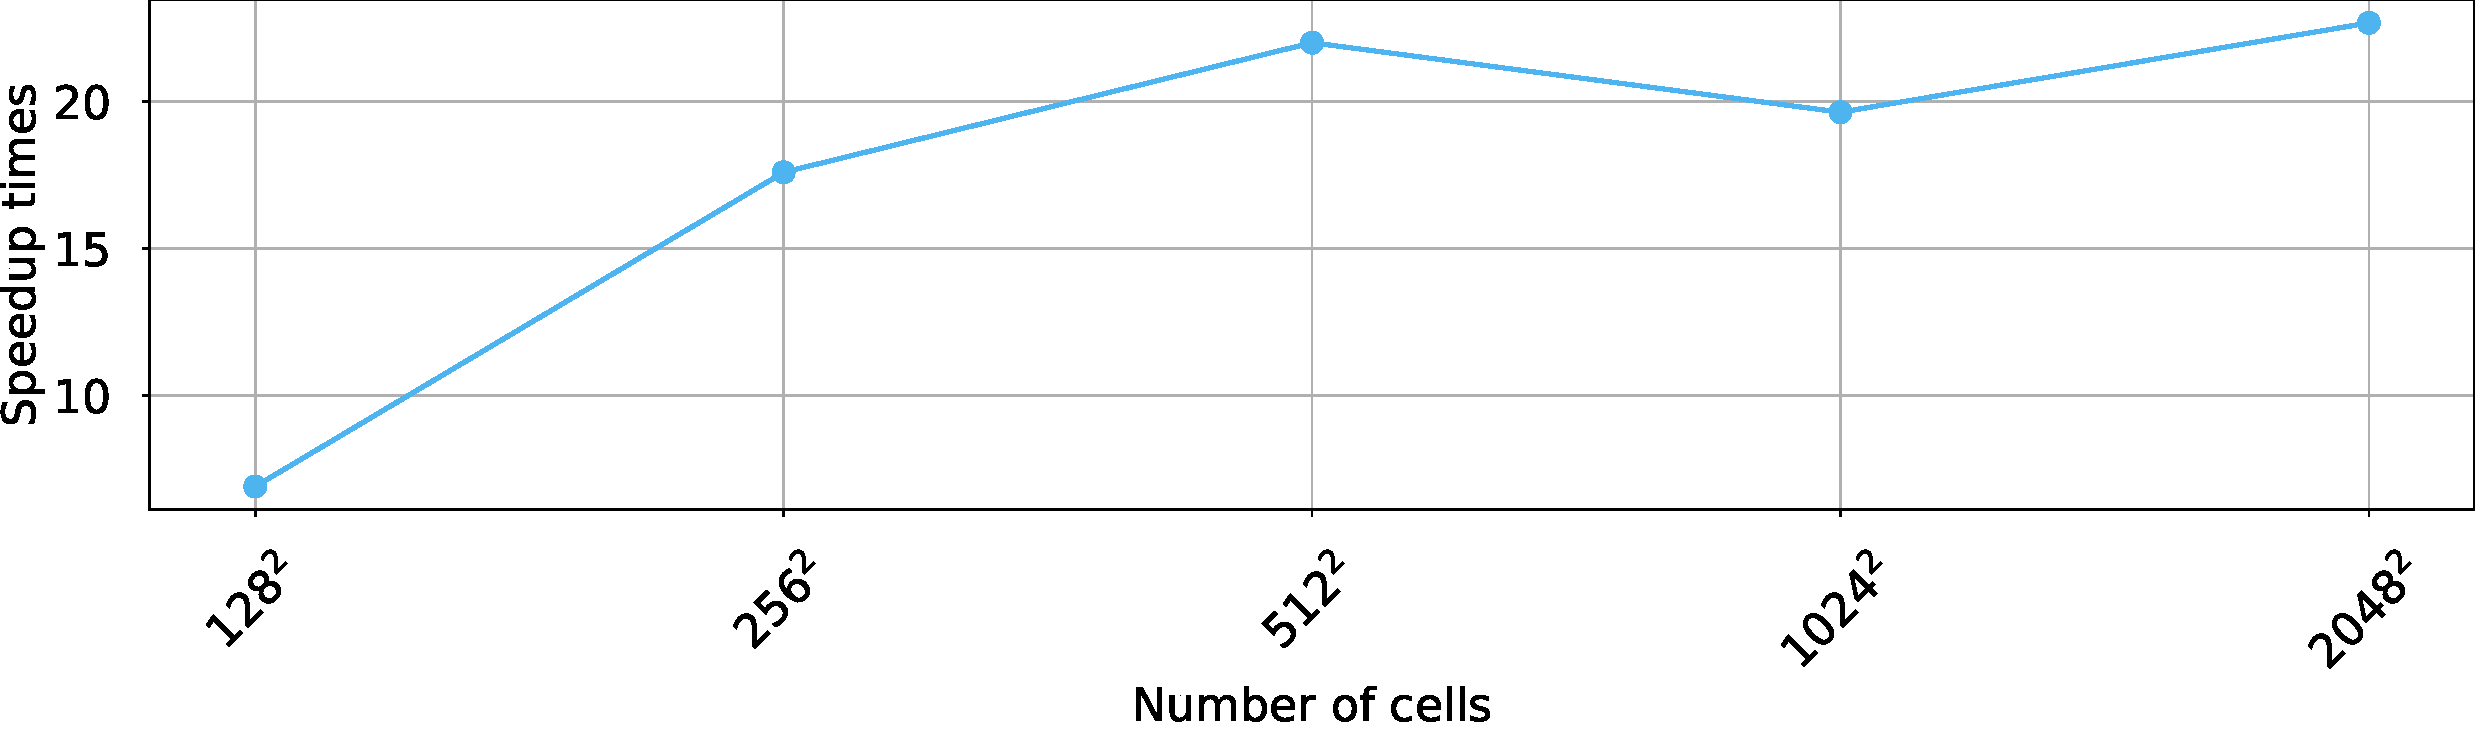
\includegraphics[width=0.85\textwidth]{results/comp_time_consumer_speedup.pdf}
        \caption{RKM scheme speedup (reference $/$ our implementation)}
    \end{subfigure}
    
    \caption{Computation time on consumer hardware}
    \label{fig:comp time consumer comparison}
\end{figure}
\FloatBarrier

In Figure \ref{fig:comp time broad comparison scaling}, the scaling value $\text{Scale}(N)$ at $N \in \{256^2, 512^2, 1024^2, 2048^2\}$ is obtained by $\text{Scale}(N) = \text{Comp}(N)/\text{Comp}(N/4)$, where $\text{Comp}(N)$ is the computation time for $N$ cells. 
Because the number of cells grows by a factor of 4 between data points and the simulation computation time is proportional to the number of cells, we would expect the scaling to be 4. However, we observe that for different integration schemes and implementations, the scalings differ. We explain the lower (better) then expected scaling for small sizes by the fact that that there is not enough computation to be done to fully utilize the entire GPU. Increasing the number of cells $N$ yields better utilization, resulting in lower scaling. This effect is more prevalent on the more capable HPC GPU hardware in Figure \ref{fig:comp time helios comparison scaling}.

% For the RKM and S-I schemes the worse then expected scaling is likely a result of increasing the number of (sub)iterations for the entire simulation caused by keeping the same timestep $\dt$ for all values of $N$. For RKM scheme this resultins in lowering the timestep. For S-I scheme this results in increasing the number of iterations needed for convergence of the Conjugate gradient method.

\FloatBarrier
\begin{figure}[!ht]
    \setlength{\subfigwidth}{0.48\textwidth}
    \setlength{\belowcaptionskip}{0.5\baselineskip}
  
    \centering
    \begin{subfigure}[t]{\subfigwidth}
        \centering
        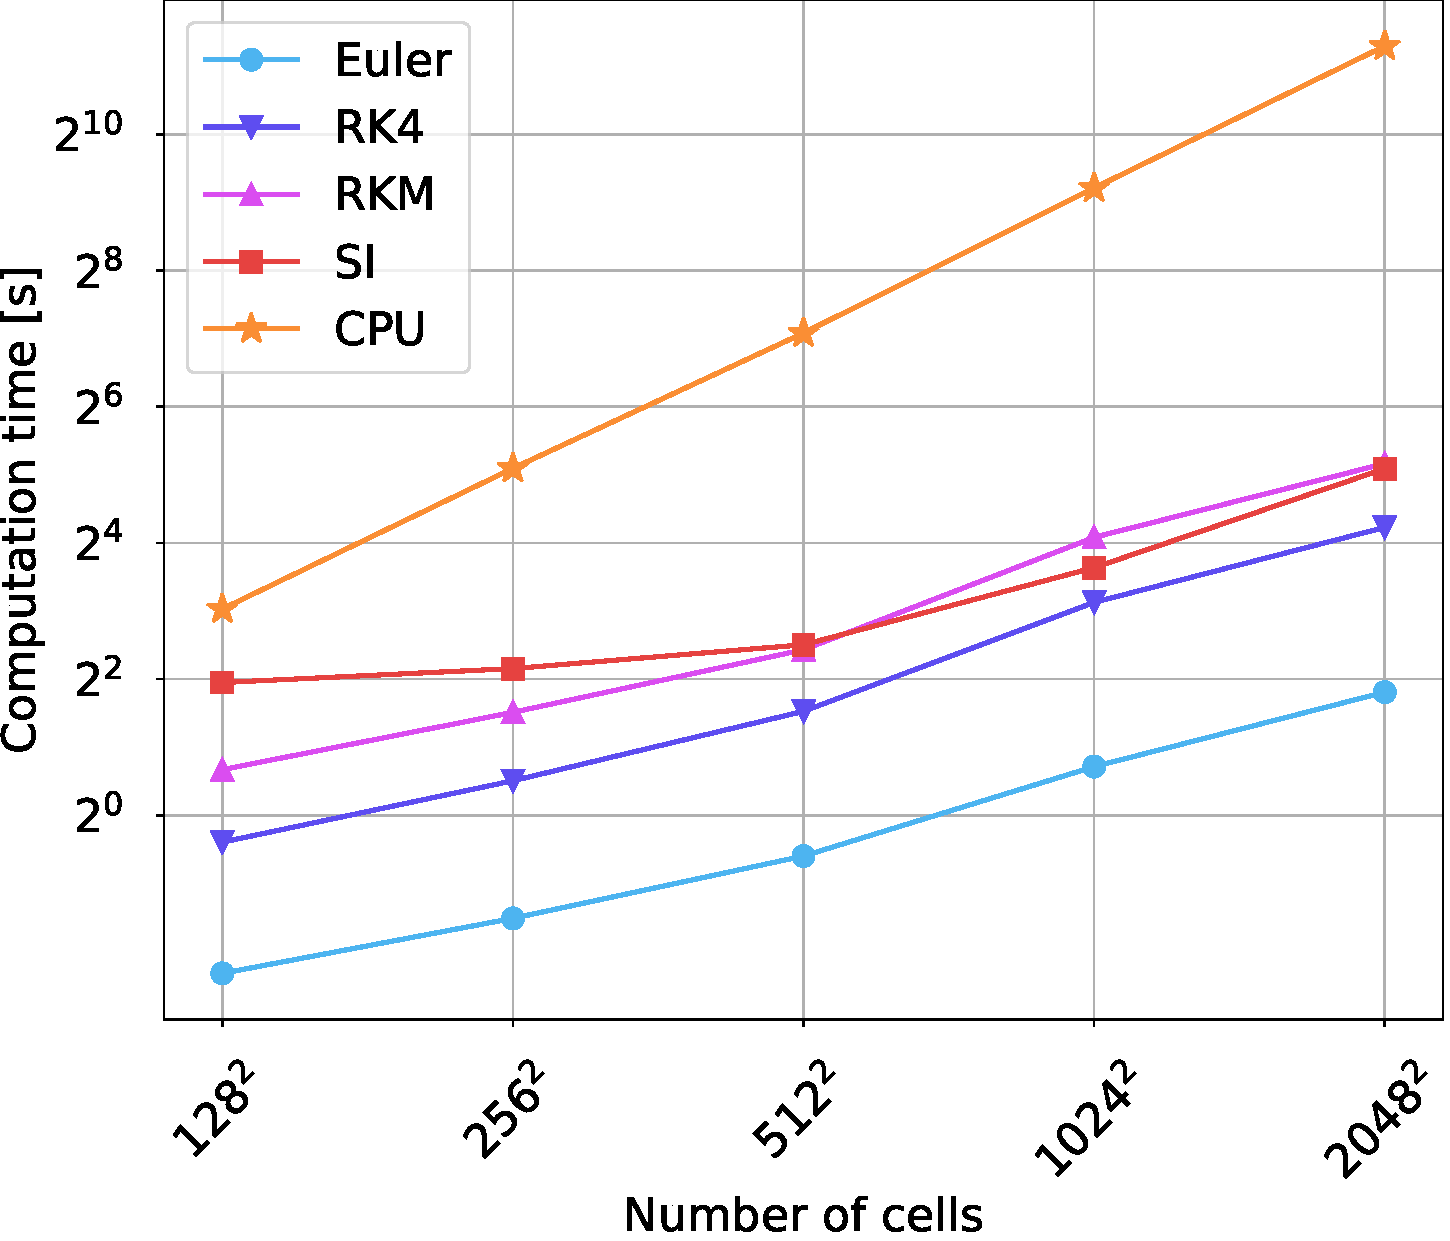
\includegraphics[width=0.95\textwidth]{results/comp_time_specialized.pdf}
        \caption{Computation time}
        \label{fig:comp time helios comparison}
    \end{subfigure}
    \hfill    
    \begin{subfigure}[t]{\subfigwidth}
        \centering
        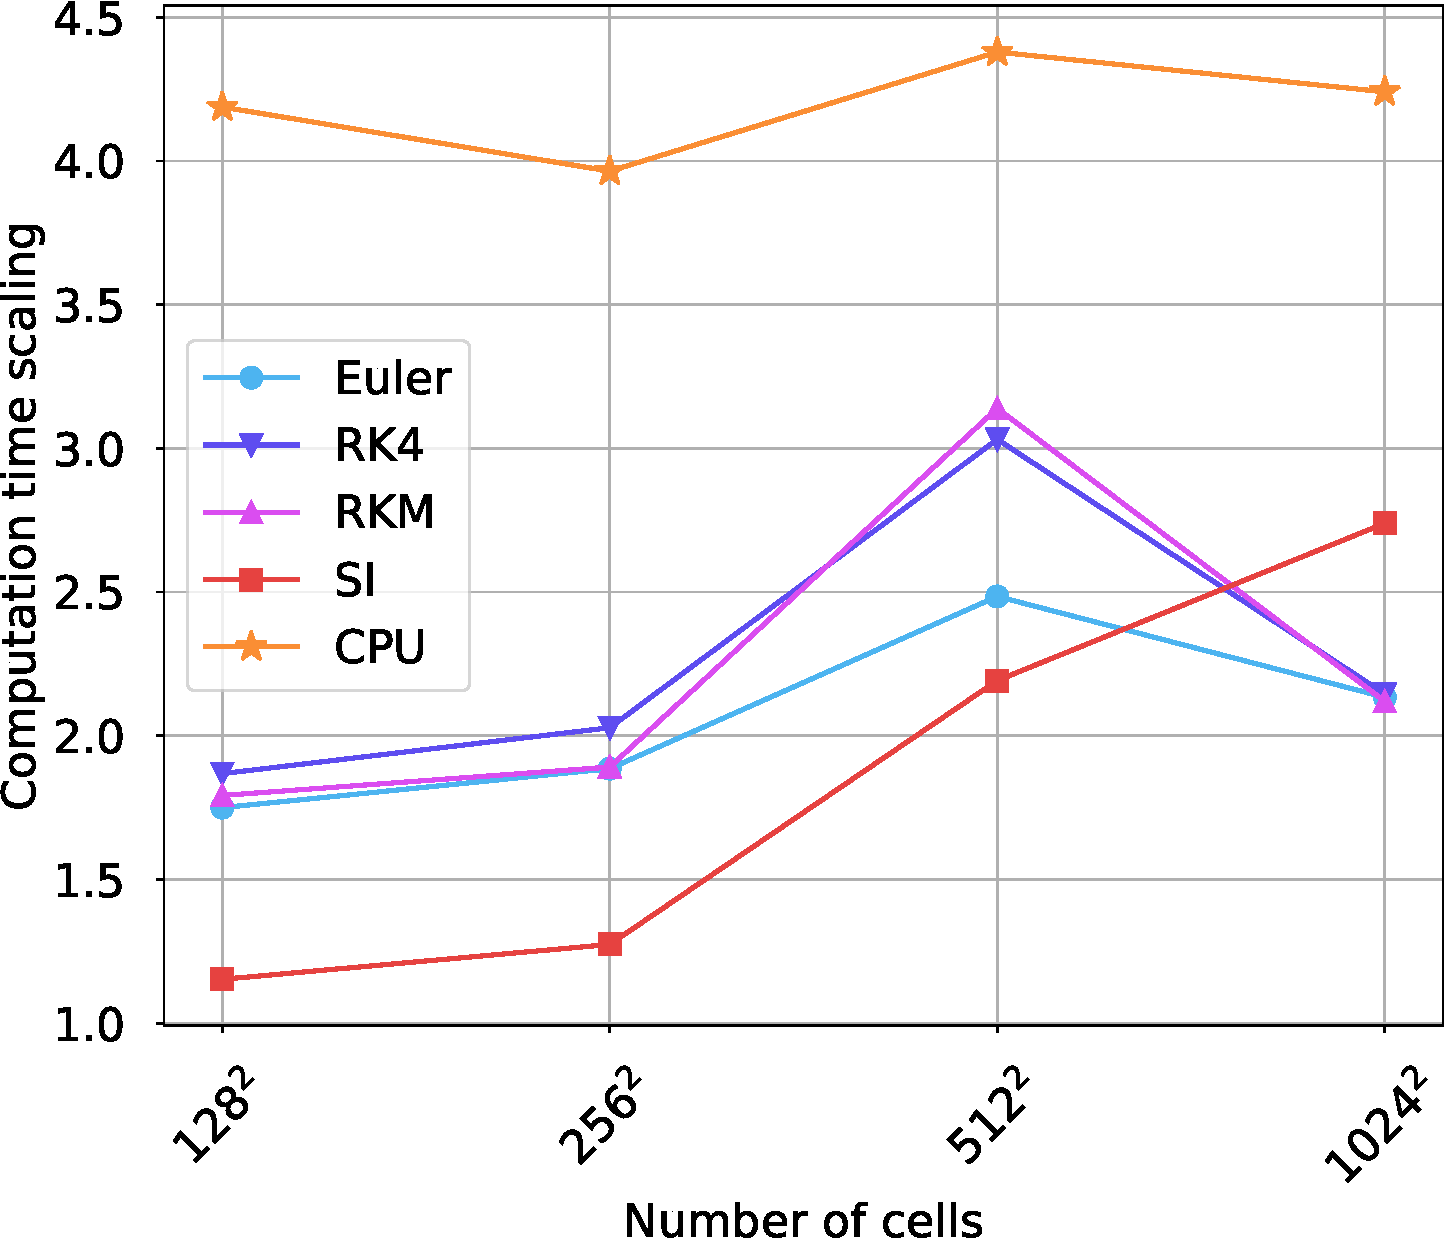
\includegraphics[width=0.95\textwidth]{results/comp_time_specialized_scaling.pdf}
        \caption{Computation time scaling}
        \label{fig:comp time helios comparison scaling}
    \end{subfigure}
    \par\vvskip
    \begin{subfigure}[t]{\textwidth}
        \centering
        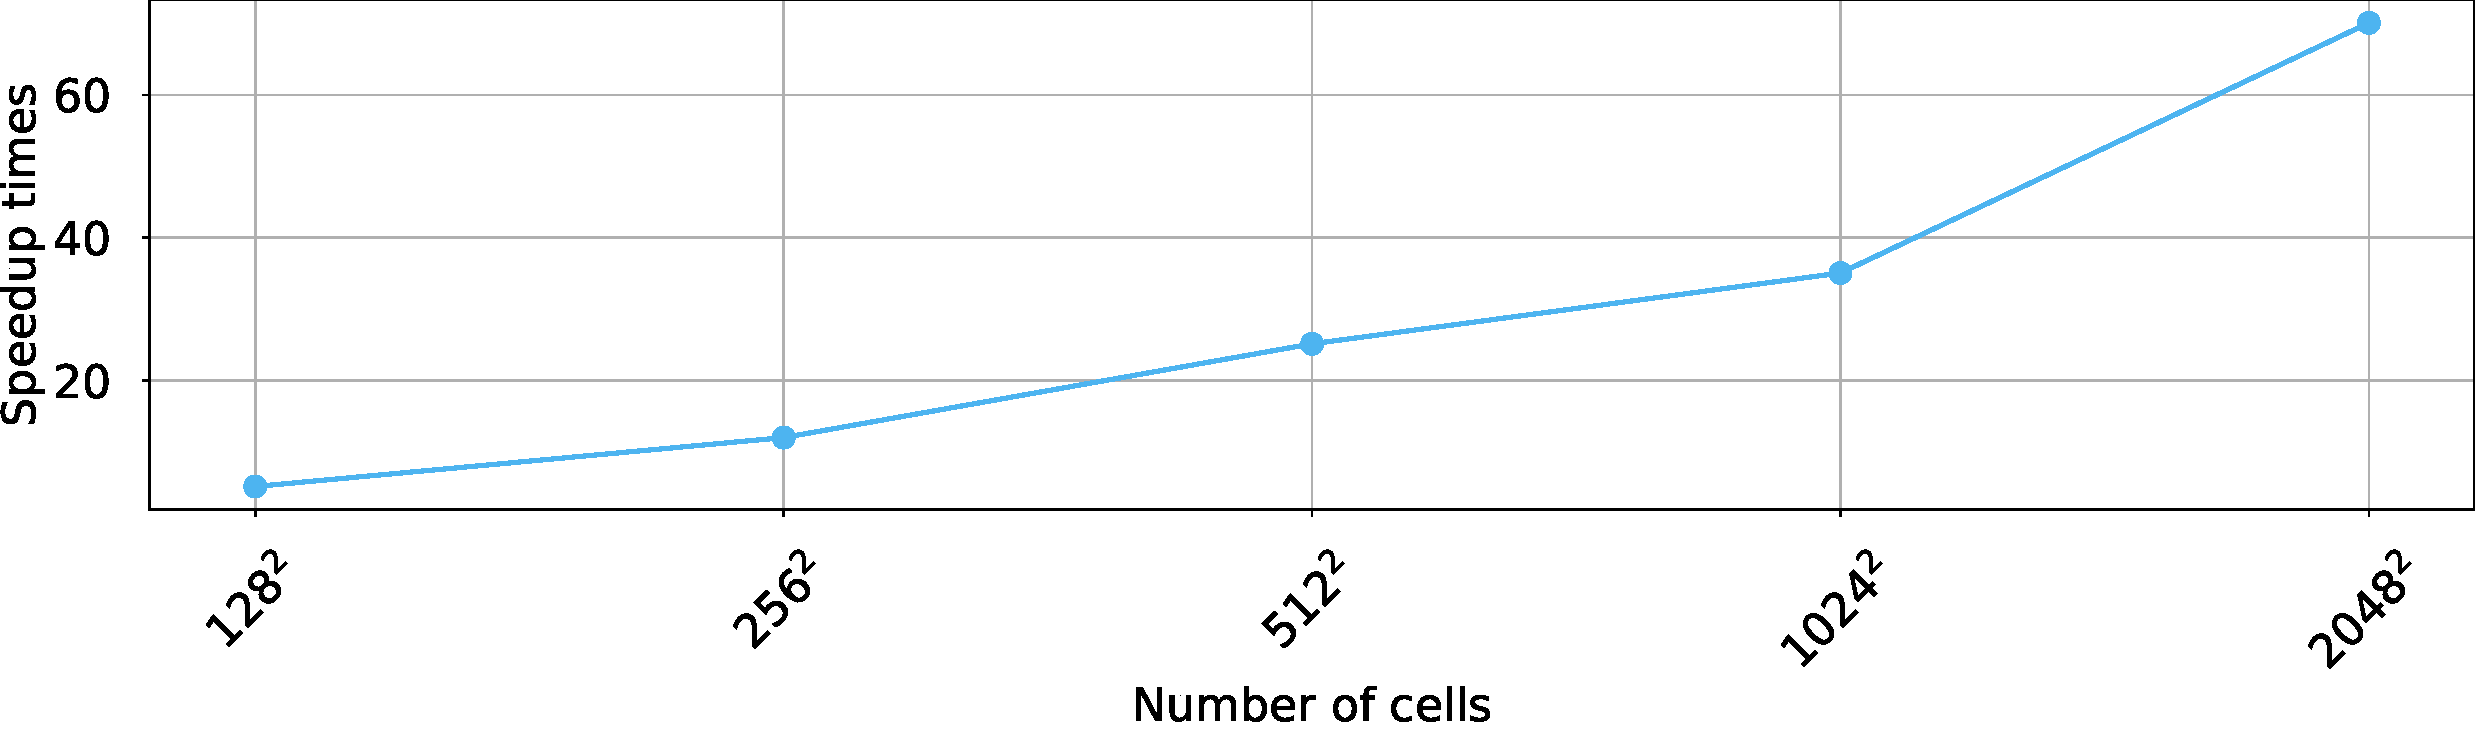
\includegraphics[width=0.85\textwidth]{results/comp_time_specialized_speedup.pdf}
        \caption{RKM scheme speedup (reference $/$ our implementation)}
    \end{subfigure}
    
    \caption{Computation time on HPC hardware}
    \label{fig:comp time specialized comparison}
\end{figure}
\FloatBarrier

% The results depicted on Figures \ref{fig:comp time helios comparison}, \ref{fig:comp time helios comparison scaling} were obtained for the simulation setup given in Section \ref{sec:simulation setup} with $S = 0$. The hardware of the supercomputer Helios was used. Specifically, a single NVIDIA Tesla V100 SXM2 w. 16GB HBM2 RAM GPU was used to run our implementation and 16-core AMD EPYC 7281@2.1GHz CPUs were used to run the reference implementation. The scaling of our implemetation behaves similarly to when running on the less powerful NVIDIA GeForce MX450 GPU depicted on Figure \ref{fig:comp time broad comparison scaling}.


% \FloatBarrier
% \begin{figure}[!ht]
%     \centering
%     \begin{subfigure}[t]{\textwidth}
%         \centering
%         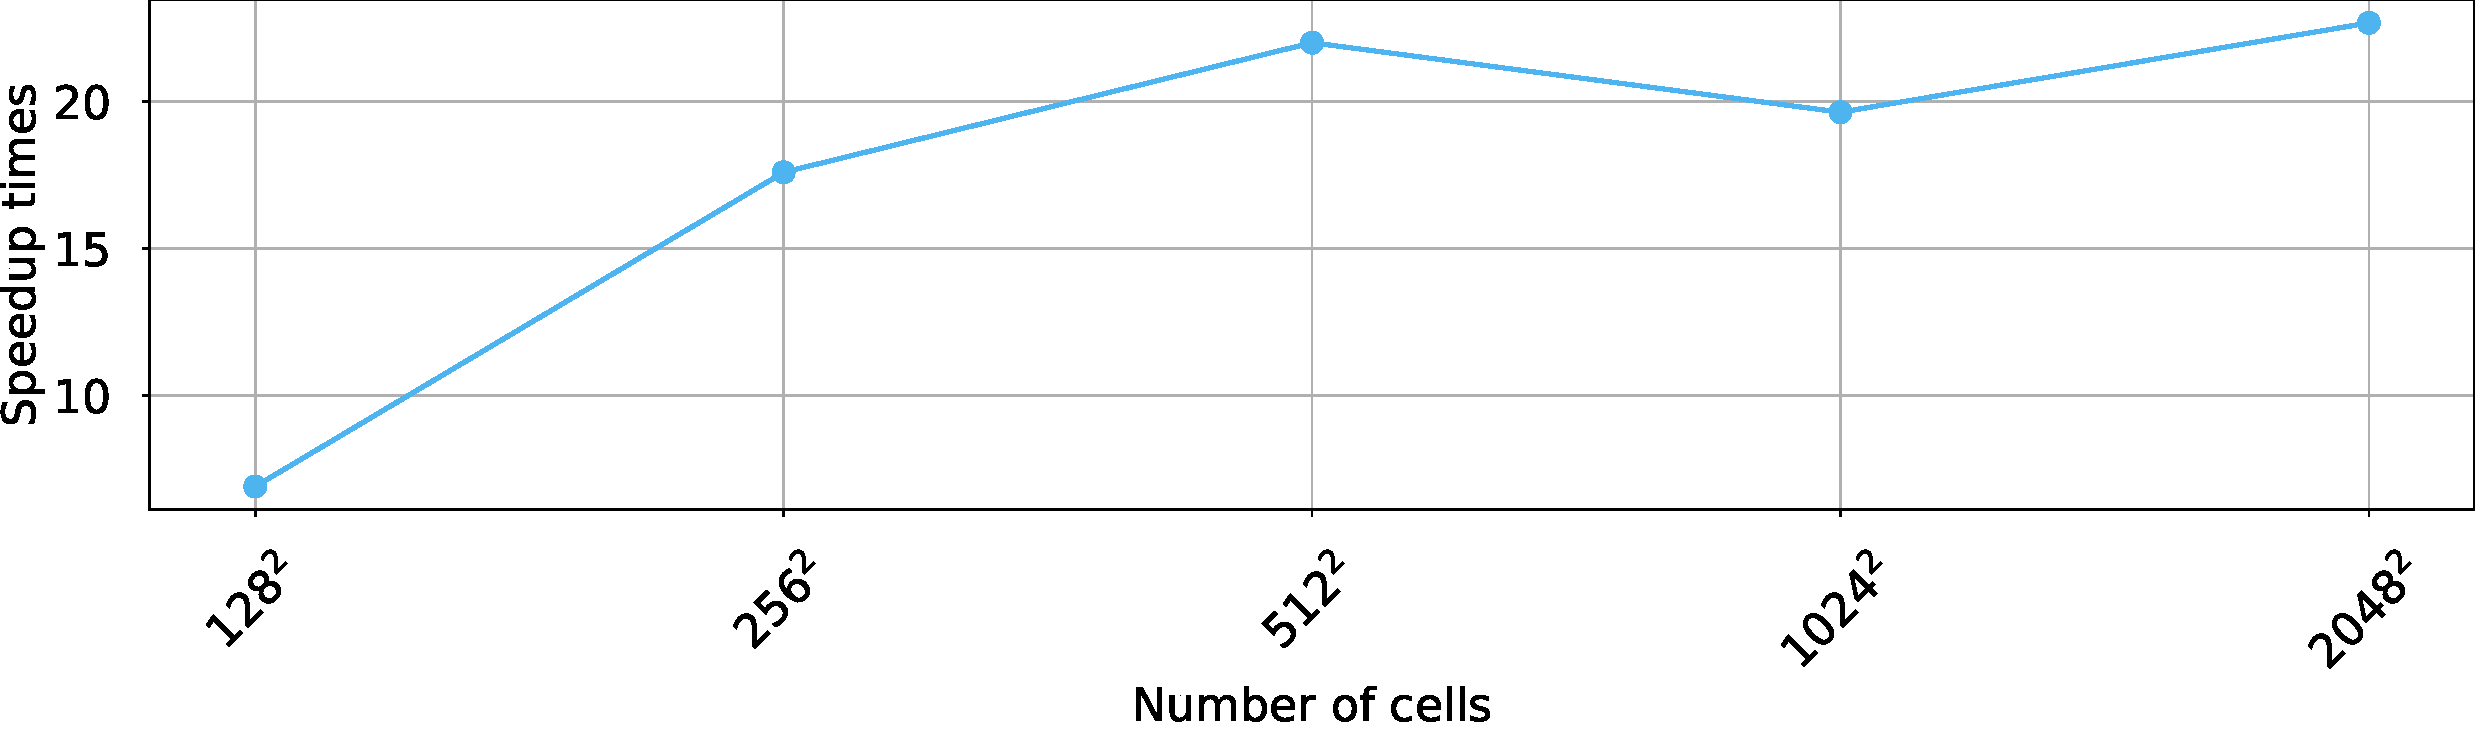
\includegraphics[width=0.7\textwidth]{results/comp_time_consumer_speedup.pdf}
%         \caption{Speedup on consumer hardware}
%     \end{subfigure}
    
%     \begin{subfigure}[t]{\textwidth}
%         \centering
%         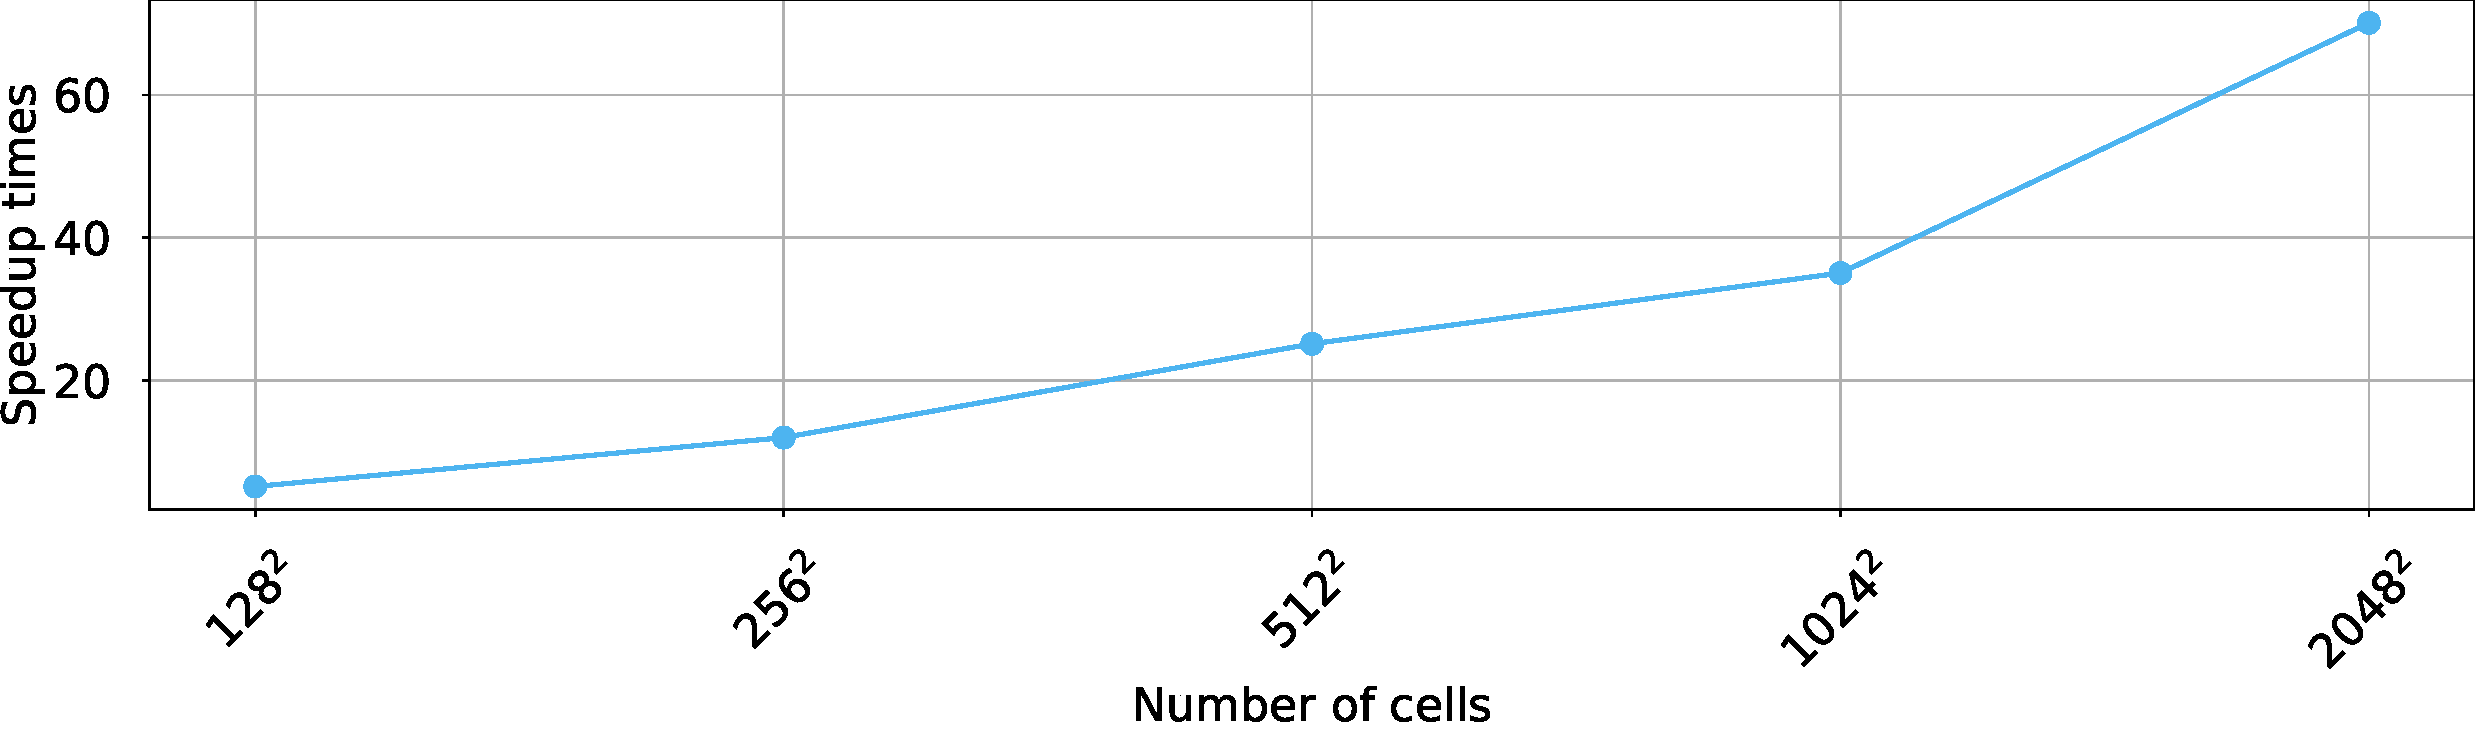
\includegraphics[width=0.7\textwidth]{results/comp_time_specialized_speedup.pdf}
%         \caption{Speedup on specialized hardware}
%     \end{subfigure}
    
%     \caption{Speedup of our implementation compared to the reference implementation. Simulation setup given in Section \ref{sec:simulation setup} with $S = 0$ and the hardware given in Section \ref{sec:algorithm benchmarks} was used.}
%     \label{fig:comp time speedup}
% \end{figure}
% \FloatBarrier

From Figure \ref{fig:comp time consumer comparison} we conclude that the goal of good simulation performance on consumer grade hardware was achieved. On the other hand, Figure \ref{fig:comp time specialized comparison} shows that the employed implementation scales well to more powerful GPU setups. 
% Still, multi-GPU implementation is required for efficient computation utilizing the whole compute cluster.

% }
\iffalse
\section{Comparison with analytical solution}
We compare the results obtained to the reference analytical solution similar to \cite{StrachotaDizertation}, with goal of establishing Experimental Order of Convergence (EOC) for the numerical methods proposed. Because the reference analytical solution \cite{Schmidt1996Exact} is given for the Sharp Interface problem (see Section \ref{sec:sharp interface problem}), we have to consider two independent limits:
\begin{enumerate}
    \item Convergence of the Phase field model to the Sharp interface model with $\xi \to 0$ \cite{Benes1997Dizertace},
    \item Convergence of the numerical solution of the Phase field model to the exact solution of the Phase field model with $\dx,\dy \to 0$.
\end{enumerate}
To correctly asses the EOC both of these limits need to be observed together. Because of this we define $\dx,\dy$ using $\xi$ and calculate the EOC using limit $\xi \to 0$.

\subsection{The sharp interface problem} \label{sec:sharp interface problem}
    We state the analytical solution for two dimensional sharp interface problem adopted from \ref{sec:correction term}. We define 
    \begin{align}
        R(t) &= \sqrt{R_{ini}^2 + 2\lambda t}, \\
        U(t) &= \bigfrac{-\epsilon(\lambda + 2)}{R(t)}, \\
        H(s) &= -\lambda e^{(\lambda/2)} \int_1^s \bigfrac{e^{-(\lambda/2)z^2}}{z^2}\dd z, \label{eq:sharp interface H} \\
        f^T(t) &= \ddt{U}(t) = \frac{\epsilon\lambda(\lambda + 2)}{R(t)^3},
    \end{align}
    for $\epsilon, \lambda, R_{ini} > 0$. 
    Using the function $d$ of distance to the nucleus center (see Section \ref{sec:setup initial conditions}), the temperature field
    \begin{align}
        \Tilde{T}(t, \vec{x}) = \begin{cases}
            U(t)                              & \vec{x} \in \Domain, d(\vec{x}) \le R(t) \\
            U(t)+H(\frac{d(\vec{x})}{R(t)})   & \vec{x} \in \Domain, d(\vec{x}) \ge R(t)
        \end{cases}
    \end{align}
    and the phase interface 
    \begin{align}
        \Gamma(t) = \left\{\vec{x} \in \Domain | d(\vec{x}) = R(t)\right\}
    \end{align}
    are the exact solution to the system
    \begin{align}
        \dert{T} &= \laplace{T} + f^T(t)                             && \text{ in } \Timeint \times \Omega, \\
        \dert{T} &= -\nu_\Gamma(t)                                   && \text{ on } \Gamma(t), \\
        \epsilon \nu_\Gamma(t) + \epsilon \kappa_\Gamma(t) + T &= 0  && \text{ on } \Gamma(t),
    \end{align}
    where $\nu_\Gamma(t) = \ddt{R(t)} = \bigfrac{\lambda}{R(t)}$ and $\kappa_\Gamma(t) = \bigfrac{2}{R(t)}$ are the normal velocity and the mean curvature of phase interface. The integral in (\ref{eq:sharp interface H}) can be rewritten as
    \begin{align}
        \int_1^s \bigfrac{e^{-(\lambda/2)z^2}}{z^2}\dd z = e^{-(\lambda/2)} - \frac{1}{s}e^{-(\lambda/2)s^2} + \sqrt{\frac{\lambda}{2}\pi}\left(\text{erf}\left(\sqrt{\frac{\lambda}{2}}\right) - \text{erf}\left(s\sqrt{\frac{\lambda}{2}}\right) \right),
    \end{align} which can be implemented using the \code{erf} function from C standard library \cite{StrachotaDizertation}.

    \subsection{The phase field formulation}
    The Phase field model given in Section \ref{sec:phase field model} does not converge to the sharp interface model \ref{sec:sharp interface problem} with $\xi \to 0$. As such a small modification has to be made which yields
    \begin{align}
    \dert{T} &= \laplace{T} + L \dert{\Phi} + f^T(t)                                    && \text{ in } \Timeint \times \Omega, \\
        \alpha\xi^2\dert{\Phi} &= \xi^2\laplace{\Phi} + f(T, \Phi, \nabla \Phi)         && \text{ in } \Timeint \times \Omega, \\
        T|_{t = 0} &= \Tilde{T}|_{t = 0}                                                && \text{ in } \Omega, \\
        \Phi|_{t=0} &= \Phi_{ini}                                                       && \text{ in } \Omega, \\
        T|_{\partial \Domain} &= \Tilde{T}|_{\partial \Domain}                          && \text{ in } \Timeint \times \partial \Omega, \\
        \nabla \Phi \cdot \vec{n} &= 0                                                  && \text{ in } \Timeint \times \partial \Omega,
    \end{align}
    where $f$ is the reaction term given by (\ref{eq:reaction term}). The numerical methods have to be adjusted accordingly, but as this change is simple to implement, it will not be discussed. 

    The model parameters are set to $a = b = \alpha = L = 1, \beta = 1/\epsilon, T^* = 0$. The initial condition for phase field is chosen $\Phi_{ini}$ using (\ref{eq:def Phi initial conditions}) with $\xi_0 = ?$. Note that this satisfies 
    \begin{align*}
        \left\{\vec{x} \in \Omega | \Phi_{ini}(x) = \frac{1}{2}\right\} = \Gamma(0).
    \end{align*}
    The homogeneous Neumann and homogeneous Dirichlet boundary conditions are used for the phase and temperature fields respectively.  

\subsection{Experimental order of convergence}

The experimental order of convergence is a tool for experimentally determining the accuracy of numerical scheme with respect to the exact solution. 

\newcommand{\EOC}[0]{\text{EOC}}

Let $(n_k) \subset \R^N$ be an increasing sequence of cell counts. Let $\Cells_{n_l}$ be a uniform mesh with $n_k$ cells in both the $\vec{e}_1$ and $\vec{e}_2$ directions each with the size $\dx = \dy = h_k$. Let $\vec{\psi}_{n_k}:\Cells_{n_k} \to \R$ be a mesh function approximating the exact solution $\vec{\psi}:\Omega \to \R$ to some system of PDE's. Let $\vec{P}_{n_k}\in \R^{n_k \times n_k}$ be a vector of values of the mesh function $\psi$ given by (\todoref). Let $\vec{P}$ be a vector of the exact solution projected onto the mesh $\Cells_{n_k}$, that is $\vec{P}_{i,j} = \psi((j-1)h_k, (i-1)h_k)$ $\forall i,j \in \hat{n_k}$.
We define the error $E_k = \norm{\vec{P} - \vec{P}_{h_k}}$ \label{eq: Ei} and \emph{experimental order of convergence} $\text{EOC}_k$ as
\begin{align}
    \text{EOC}_k = \log{\left( \bigfrac{E_k}{E_{i-1}} \right)} / \log{\left( \bigfrac{h_k}{h_{i-1}} \right)} \forall k \in \Nats.
\end{align}

Because the phase field model is described in time and two spatial dimensions we perform the norm in the definition of $E_k$ as
\begin{align}
    E_k = \max \limits_{t \in \hat{\Timeint}} \norm{\vec{P}(t) - \vec{P}_{h_k}(t)} \label{eq: Ei 2D-time}
\end{align}
where $\hat{\Timeint}$ is discretization of the time interval $\Timeint$ into time steps. 

In the following experiments we set $\Omega = (0,4)^2$, $x_0 = (2,2)$, $R_{ini} = 0.25$, 
$\Timeint = [0, 0.75]$, $h_k = 4/256i$, $\dx = \dy = h_k$, $\xi_k = \bigfrac{11}{10}h_k$, $\lambda = 0.5$, $\epsilon = 0.0001$. $\vec{P}(t)$
is replaced with the phase field $\Phi$ and temperate field $T$ evaluated at each of the cell centroids. The phase value norm \todoref and $\norm{\cdot}_2$ were used in (\ref{eq: Ei 2D-time}) for phase and temperature fields respectively. 
The resulting EOC tables are given in \todoref and \todoref. A figure comparing the resulting crystal shapes for $h_k = 4/2048$ is shown in figure \todoref.

\fi

\chapter*{Conclusion}

\pagestyle{plain}

\addcontentsline{toc}{chapter}{Conclusion}

This work presents the derivation of several numerical schemes for solving the two dimensional phase field problem with a simple anisotropy, together with its GPU parallel implementation showing good performance on consumer hardware. The finite volume method notation is introduced and utilized to derive approximations for the Laplacian and gradient differential operators on admissible meshes. Different boundary conditions are described within the finite volume framework using ghost cells. Semi-discrete scheme of the phase field model is derived. Then explicit time integration schemes such as the explict Euler and Runge-Kutta-Merson methos are discussed and a time integration algorithm is presented. Semi-implicit time integration scheme utilizing the Crank-Nicolson method is derived. Solution of the resulting matrix of equations is discussed and operator splitting method is utilized to aid numerical matrix solvers and enabling the conjugate gradient method to be used. Internal error introduced by the operator splitting method is quantified and two techniques are provided for its reduction. The first is the repeated iteration technique, which has been shown to reliably reduce the operator splitting error. The second is the correction term technique, which has failed to reduce the operator splitting error, but produces similar crystal structures to the repeated iteration technique at no additional runtime cost. 

Next, a detailed introduction to the CUDA hardware and programming model is given. Even though the text starts with simple examples, it quickly reaches non-trivial optimized implementations of the parallel for, parallel tiled for and parallel reduction algorithms. Special focus is put on shared memory with relation to the CUDA programming model and optimization of memory intensive kernels. A state-of-the-art parallel reduction kernel is presented, utilizing warp-level parallelism. Benchmarks of the presented algorithms are performed, showcasing superior performance on small and large datasets compared to the CUDA Thrust library.

Finally, simulation results of the proposed time integration schemes are shown. A discussion of boundary conditions and their impact on the simulation is given. Integration schemes are compared, showcasing consistency between the different techniques. The runtime performance of the developed simulation code is compared against a reference implementation. Speedups upwards of 20 times can be observed on both consumer hardware and specialized HPC hardware. The developed simulation code is freely available at \href{https://github.com/Boostibot/bachelors}{https://github.com/Boostibot/bachelors}. 

Further work is needed to extend the proposed algorithms to three dimensions and efficiently distribute the simulation workload in many GPU setups, enabling simulation on high resolution three dimensional meshes. 
The parallel algorithms developed in this work can be used with advantage to solve more complex models including, for example, phase transitions in alloys, solidification subject to fluid flow, or freezing and thawing in porous media.









\printbibliography

% \begin{thebibliography}{1}


% \bibitem{Allen-Cahn}S. Allen, J. W. Cahn: \emph{A microscopic theory for antiphase boundary motion and its application to antiphase domain coarsening}. Acta Metall., 27:1084-1095, 1979.
% \bibitem{cit: PF in engineering}N. Provatas, K. Elder, \emph{Phase-Field Methods in Materials Science and Engineering}, WILEY-VCH Verlag GmbH \& Co. KGaA, 2010.
% \bibitem{ProvetasElder2010}Y. Wang et al., \emph{Simulation of Microstructure Evolution in Mg Alloys by Phase-Field Methods: A Review}, Crystals (12), 2022, 1305.
% \bibitem{Strachota_dendric_crystal}P. Strachota, A. Wodecki, M. Beneš, \emph{Focusing the latent heat release in 3D phase field simulations of dendritic crystal growth}. Modelling Simul. Mater. Sci. Eng. 29 065009 (2021). ISSN: 0965-0393.
% \bibitem{cit: PF in material science}I. Steinbach, \emph{Phase-field models in materials science}, Modelling Simul. Mater. Sci. Eng. (17), 2009, 073001.
% \bibitem{High Perf GPU}T. Takaki, S. Sakane, R. Suziki, \emph{High-performance GPU computing of phase-field lattice Boltzmann simulations for dendrite growth with natural convection}. IOP Conf. Series: Materials Science and Engineering 1281 (2023), 012056.
% \bibitem{MoukalledFVM2016}F. Moukalled, L. Mangani, M. Darwish et al., \emph{The finite volume methods in computational fluid dynamics}. Springer, 2016.
% \bibitem{J.Palan}J. Palán, \emph{Modely fázového pole v materiálových vědách a jejich numerické řešení}. Diplomová práce, FJFI ČVUT v Praze, 2023.
% \bibitem{BenesSolidification2001}M. Beneš, \emph{Mathematical and computational aspects of solidification of pure substances}. Acta Math. Univ. Comenian. (N.S.),70(1), 123–151, 2000.
% \bibitem{Caginalp1989}Caginalp G 1989 Phys. Rev. A \href{https://journals.aps.org/pra/abstract/10.1103/PhysRevA.39.5887}{39 5887–96}
% \bibitem{Kobayashi1993}Kobayashi R 1993 Physica D 63 \href{https://www.sciencedirect.com/science/article/abs/pii/016727899390120P?via%3Dihub}{410–23}
% \bibitem{CUDA}NVIDIA Corporation,\emph{CUDA C++ Programming Guide}, Release \href{https://docs.nvidia.com/cuda/pdf/CUDA_C_Programming_Guide.pdf}{12.5}, 2024, Retrieved 2024-08-5.
% \bibitem{StrachotaDizertation} \TODO{!}
% \bibitem{ChristiansenRKM1970}J. Christiansen, \emph{Numerical solution of ordinary simultaneous differential equations of the 1st order using a method for automatic step change}, Numer. Math. 14 (1970), 317–324.

% \end{thebibliography}

\end{document}
